\documentclass[11pt]{article}
\usepackage[utf8]{inputenc}
\usepackage{amsmath,amssymb,amsfonts,amsthm}
\usepackage{graphicx}
\usepackage{xcolor}
\usepackage{hyperref}
\usepackage{tikz}
\usetikzlibrary{calc, arrows.meta, decorations.markings, patterns, shapes.geometric, positioning, 3d, decorations.pathmorphing}
\usepackage{geometry}
\usepackage{booktabs}
\geometry{margin=1in}
\newenvironment{acknowledgments}
  {\section*{Acknowledgments}}
  {}
% ===== BIBLIOGRAPHY - CHOOSE ONE OPTION =====

% OPTION 1: Use natbib (recommended for Springer)
%\usepackage[numbers,sort&compress]{natbib}

% OPTION 2: Use cite (simpler, also works)
\usepackage{cite}

% ===== DON'T USE BOTH! =====

% Theorem environments
\newtheorem{theorem}{Theorem}
\newtheorem{lemma}{Lemma}
\newtheorem{proposition}{Proposition}
\newtheorem{corollary}{Corollary}
\newtheorem{definition}{Definition}
\newtheorem{remark}{Remark}

\begin{document}

\title{A Theoretical and Computational Implementation of a Participatory ``It From Bit'' Universe}

\author{
  Robert C. Dennis\thanks{Corresponding author. Email: cdenn016@gmail.com}\\[0.3cm]
  \small Independent Researcher\\
  \small Leander, Texas, United States\\[0.2cm]
  \small ORCID: \href{https://orcid.org/0009-0004-4688-2341}{0009-0004-4688-2341} % ← Add your ORCID if you have one, otherwise remove this line
}

\date{\today}

\maketitle

\begin{abstract}
We construct a gauge theory of variational inference on a principal $G$-bundle and use it to give mathematical content to several proposals that have circulated as informal philosophy: Wheeler's "it from bit", Kant's phenomenal/noumenal distinction, and Lahav and Neemeh's recent argument that phenomenal consciousness is a frame-relative quantity. Agents are smooth sections of an associated bundle carrying beliefs $q(c)$, priors $p(c)$, and gauge frames $\phi(c)$ over a base manifold. Inter-agent interaction is mediated by gauge-covariant transport operators $\Omega_{ij} = e^{\phi_i}e^{-\phi_j}$, with coupling strengths given by a softmax over Kullback-Leibler divergences. Dynamics arise from natural-gradient descent on a global variational free energy. The construction yields four results. First, in the 0-dimensional limit it recovers standard transformer attention, and the resulting architecture is a working language model when trained without learned attention projections, MLPs, or pointwise activation functions; multi-seed validation on WikiText-103 across embedding dimensions $K \in [10, 120]$ and three independent seeds, at an iso-token budget of $122.9$M tokens, exhibits clean power-law scaling $\mathrm{PPL} = aK^b + c$ with $b = -1.05$ (95\% bootstrap CI $[-1.10, -1.00]$) and $R^2 = 1.000$ on the per-$K$ seed means. Second, agent gauge frames provide an explicit transformation law between cognitive reference frames in the sense of Lahav and Neemeh, supplying the group action and frame-invariant quantity their account requires but does not write down. Third, multi-scale meta-agent dynamics with bidirectional consensus run in working simulations. Fourth, in a linearized 2D worked example with an imposed imaginary temporal generator (acknowledged as a postulate, not a derivation), $\mathrm{GL}(K, \mathbb{C})$ gauge frames produce indefinite pullback metrics structurally compatible with a Lorentz subgroup $\mathrm{SO}(1,1)$, and a real-Lorentzian metric is recovered after a real-part projection; the four-dimensional, fully nonlinear extension and the dynamical selection of the imaginary generator are left open (see Section~\ref{sec:signature_resolution}). The framework does not yet predict physical constants, does not yet contain a rigorous quantum extension, and does not solve the hard problem of consciousness so much as relocate it; these limitations are stated explicitly in Section~\ref{sec:scope_limitations}. What it does provide is a mathematical setting in which observer-dependent reality, frame-relative experience, and information-theoretic emergence of geometric structure can be studied without leaving rigorous ground.
\end{abstract}

\noindent\textbf{Keywords:} Gauge theory $\cdot$ Active inference $\cdot$ Free energy principle $\cdot$ Information geometry $\cdot$ Emergent spacetime $\cdot$ Transformer architectures

\section{Introduction}

\subsection{Wheeler's Vision}

In 1990, John Archibald Wheeler posed one of the most profound questions in the foundations of physics: "How come existence?" His answer, encapsulated in the phrase "it from bit", suggested that physical reality derives its existence from information~\cite{Wheeler1990}. Wheeler argued that the universe is participatory such that the act of observation does not merely reveal pre-existing reality but actively participates in bringing that reality into being. As he wrote, "no phenomenon is a phenomenon until it is an observed phenomenon"~\cite{Wheeler1983}.

This vision extends beyond quantum mechanics to a cosmological scale. Wheeler proposed that the universe is engaged in a self-referential bootstrap such that observers emerge from physical processes, yet those same observers participate in defining the physical laws and structures from which they arose. The universe, in this view, is not a pre-existing mathematical structure waiting to be discovered, but an evolving informational system where "law without law" emerges through participatory dynamics~\cite{Wheeler1983}.

Despite its profound implications, Wheeler's vision has remained largely philosophical. While quantum information theory has formalized the "bit"~\cite{Shannon1948,CoverThomas2006}, and while active inference frameworks have modeled observer behavior~\cite{Friston2010,Friston2017}, no rigorous mathematical framework has united these threads to show how "it" can computationally emerge from "bit".

\subsection{The Kantian Foundation}

Wheeler's participatory universe finds deep philosophical resonance with Immanuel Kant's radical proposal in his 1781 \emph{Critique of Pure Reason}~\cite{Kant1781}. Kant argued convincingly that space and time are not properties of things-in-themselves (the noumena), but rather "forms of sensuous intuition": fundamental constructions of the perceiving mind that organize raw sensory data into coherent experience. In Kant's framework, we can never access the noumenal reality directly; all experience is mediated through the cognitive apparatus that structures perception.

This philosophical insight lay dormant in physics for over a century until Hermann von Helmholtz proposed the first practical advance: the brain as an "unconscious inference" machine~\cite{Helmholtz1867}. Helmholtz argued that perception is a process of statistical inference, where the brain constructs the most probable interpretation of ambiguous sensory data. This proto-Bayesian framework anticipated modern predictive processing theories by more than a century.

In the 2000s, Karl Friston revolutionized this picture with his Free Energy Principle~\cite{Friston2010}. By deriving perception, action, and learning from a single variational free energy functional, Friston demonstrated that biological systems can be understood as performing approximate Bayesian inference to minimize surprise. Active inference (the extension incorporating action as inference about how to sample the world) has since exploded into a comprehensive framework encompassing neuroscience, psychology, and artificial intelligence~\cite{Parr2022}.

Yet despite these profound advances in understanding perception as statistical construction, they have remained confined to cognitive science and neuroscience. The physics community, meanwhile, has pursued an independent trajectory.

\subsection{The Physics Revolution: Emergent Spacetime}

Physics has undergone its own conceptual upheavals regarding the nature of spacetime. General relativity treats spacetime as a dynamical entity, but still presupposes it as the fundamental arena in which physics unfolds. In the 1970s, this assumption came under attack as physicists attempted to reconcile quantum mechanics with gravity. String theory, loop quantum gravity, and other approaches to quantum gravity suggested that spacetime itself might be an emergent, effective description arising from more fundamental quantum degrees of freedom~\cite{Carlip2014}.

A surprising discovery came in 1995 when Jacobson demonstrated that Einstein's field equations could be derived from thermodynamic principles applied to local causal horizons~\cite{Jacobson1995}. The equations governing gravity appear to be statements about entropy and information flow, suggesting that spacetime geometry has an information-theoretic origin. This insight has been reinforced by Padmanabhan's thermodynamic formulation~\cite{Padmanabhan2010}, holographic principles~\cite{Bousso2002}, the AdS/CFT correspondence~\cite{Maldacena1999}, and entanglement-based approaches to gravity~\cite{VanRaamsdonk2010}.

More recently, the ER=EPR conjecture~\cite{MaldacenaSusskind2013} and tensor network models~\cite{Swingle2012} have suggested that entanglement structure in quantum systems directly encodes geometric relationships. Spacetime, in these frameworks, emerges from patterns of quantum information and correlation. Yet despite these theoretical advances, experimental validation remains elusive, and the connection to observer-dependent reality remains unexplored.

\subsection{The Unspoken Tension}

Due to these discoveries and realisations there exists an implicit, unspoken tension in our contemporary understanding of reality. Neuroscientists and philosophers, following Kant and Helmholtz through to Friston, argue that reality is a perceptual construction. The weaker version of this claim is the predictive-processing view of perception as a "controlled hallucination" that nevertheless approximately tracks action-relevant external structure~\cite{Clark2016,Seth2021}. The stronger version, Hoffman's Interface Theory of Perception~\cite{Hoffman2019}, argues that evolved perception is selected for fitness rather than veridicality and need bear no faithful relation to the noumenal substrate at all. The framework developed below sits between the two readings rather than endorsing the strongest version of either: different agents pull back different geometries from the same noumenal substrate, and there is no agent-independent "correct" geometry, but the framework does not commit to the substrate being structurally inaccessible in Kant's sense or to evolved perception being decoupled from veridicality in Hoffman's sense. The relevant commitment is structural rather than metaphysical whereby phenomenal experience is treated as gauge-frame-dependent in its presentation and predictable, repeatable patterns about which agents form consensus emerge from the variational dynamics rather than from a stipulation about the reachability of the substrate.

Physicists, meanwhile, have long argued and hoped to find a physical explanation for consciousness, perception, and life, with limited success. The hard problem of consciousness~\cite{Chalmers1995} remains intractable when approached from a purely physical substrate. Attempts to derive experience from neuronal dynamics, quantum coherence in microtubules~\cite{HameroffPenrose1996}, or integrated information~\cite{Tononi2008} have not resolved the explanatory gap between objective description and subjective experience.

This dichotomy suggests two radical possibilities: either \emph{physics produces cognition}, or \emph{cognition produces physics}. The former physicalist program has been studied extensively for centuries with profound yet incomplete results. The latter cognitive-first ontology has been largely neglected, dismissed as idealism or solipsism. Yet Wheeler's participatory universe, Kant's transcendental idealism, and the modern variational free energy principle all point toward this neglected alternative: that physical structure, including spacetime itself, is the product of information processing by informational agents.

\subsection{A Cognitive-First Framework}

We present a mathematical framework for multi-agent interaction that takes cognitive construction seriously. Building on gauge theory, information geometry, and variational free energy, we model agents as smooth sections of principal bundles carrying beliefs $q(x)$, priors $p(x)$, and gauge frames $\phi(x)$, together with a slow subsystem of generative models $s(x)$ and model hyper-priors $r(x)$ developed in Section~\ref{sec:framework}. These agents interact through information-theoretic couplings that minimize variational free energy.

This framework produces several emergent phenomena:
\begin{enumerate}
\item Spacetime-like structure emerges from pullbacks of agent beliefs to a noumenal base manifold, inducing Fisher information metrics that decompose into observable, subthreshold informational, and internal sectors

\item Causality emerges from gauge-covariant transport operators defining information flow between agents
\item Physical laws emerge as information-theoretic necessities (e.g., the second law from non-negative KL divergence)
\item Hierarchical structure emerges through multi-scale renormalization with participatory feedback (demonstrated under threshold-based detection; see Section~\ref{sec:meta_agent_threshold})
\item Standard transformer attention emerges as the zero-dimensional limit, providing empirical validation
\end{enumerate}

The framework realizes Wheeler's "it from bit" vision mathematically. It bridges Kant's epistemological insight (that space and time are cognitive constructions) with modern physics and machine learning. Rather than deriving cognition from physics, we derive physics-like structures from information-processing agents.

\subsection{Epistemic Status}

This work operates at three distinct epistemic levels:

\textbf{Level 1: Validated Results.} Transformer attention mechanisms emerge as the zero-dimensional limit of the gauge-theoretic variational inference (Section~\ref{sec:transformers}). Two empirical layers support the derivation. (a) A small-scale single-seed study on WikiText-2 (character-level, embedding dimension 11, context length 32) achieves $r = 0.821$ correlation with BERT attention patterns and $20\%$ lower perplexity than baseline despite $25\%$ fewer parameters; this is a proof-of-principle, not a statistical claim, and seed/CI/test-split details are deferred to the companion paper~\cite{Dennis2025trans}. (b) A controlled multi-seed scaling study on WikiText-103 (Section~\ref{sec:scaling_validation}) sweeps embedding dimension $K$ over eleven values in $[10, 120]$ with three seeds at iso-token budget $122.9$M tokens and fits $\mathrm{PPL} = aK^b + c$ with $b = -1.049$ (95\% bootstrap CI $[-1.103, -0.998]$), $R^2 = 1.000$. The scaling exponent is the architectural fingerprint of the gauge-theoretic model and is robust across datasets (Japanese Wikipedia at $\sim$1B tokens reaches PPL 15--30 at comparable $K$, indicating the WikiText-103 floor reflects undertrained convergence rather than a structural ceiling).

\textbf{Level 2: Mathematical Implementation.} We have constructed and computationally implemented participatory dynamics (Sections~\ref{sec:framework}--\ref{sec:participatory}). Our Ouroboros Tower demonstrates bidirectional information flow: agents form meta-agents through consensus (bottom-up), while meta-agents propagate priors downward (top-down). This runs in working code for systems of 200 agents across 25 hierarchical scales.

\textbf{Level 3: Speculative Physical Interpretation.} We explore whether this structure might describe physical reality (Sections~\ref{sec:pullback}, \ref{sec:observer}, \ref{sec:implications}). The pullback construction induces Riemannian metrics from information geometry under the $\mathrm{SO}(3)$ restriction used in our simulations. The natural $\mathrm{GL}(K)$ gauge symmetry and its complexification $\mathrm{GL}(K, \mathbb{C})$ make Lorentzian-signature subgroups available, and Section~\ref{sec:signature_resolution} exhibits a 2D worked example in which an indefinite bilinear form is obtained after additionally postulating an imaginary frame component along a designated temporal direction and a real-part projection. Whether free-energy minimisation actually selects this configuration, and whether the construction extends beyond the linearised 2D regime, are open. Other critical problems remain unaddressed: dimensional analysis between information and physical units is incomplete, and quantum connections require further development. These sections explore mathematical possibilities, not established physics.

\textbf{Our Contribution.} Wheeler's participatory universe and Kant's phenomenal/noumenal distinction have remained informal philosophy. We provide rigorous mathematical formalism making these ideas concrete. The framework is computationally tractable (it runs), empirically constrainable (transformer validation), and mathematically coherent (gauge-covariant dynamics). Whether it describes physical reality remains open.

\subsection{Scope and Limitations}
\label{sec:scope_limitations}

The reader should hold the claims that follow to a clearly delimited scope. The framework derives a transformer architecture from gauge-theoretic variational inference, validates it empirically as a working language model, and provides mathematical structure for several interpretive moves that have circulated as informal philosophy such as  Wheeler's participatory universe, Kant's phenomenal/noumenal distinction, observer-dependent reality, and the Lahav--Neemeh proposal that consciousness is a frame-relative quantity. We do not claim to have derived quantum mechanics or general relativity from first principles, and several of the speculative results are demonstrated only at the level of worked examples. The honest delimitation:

\textbf{Validated.} The 0-dimensional gauge theory recovers standard transformer attention (Section~\ref{sec:transformers}); the resulting architecture is a working language model trained without learned attention projections, MLPs, or pointwise activation functions, with multi-seed scaling on WikiText-103 fitting $\mathrm{PPL} = aK^b + c$ at $b = -1.05$.

\textbf{Demonstrated in working code (single illustrative run).} The bidirectional Ouroboros Tower simulations of meta-agent emergence (Section~\ref{sec:participatory}) run in working code for hundreds of agents across tens of hierarchical scales, conditional on the threshold-based consensus detector of Section~\ref{sec:meta_agent_threshold}. The variational free-energy improvement criterion that this detector approximates (Section~\ref{sec:meta_agent_variational}) is not itself evaluated continuously in the simulation; whether the discrete detector and the continuous variational rule produce the same hierarchical organisation is open.

\textbf{Worked example only.} The Lorentzian-signature construction (Section~\ref{sec:signature_resolution}) is established in a 2D linearized toy model with a constant generator. The extension to four-dimensional, fully nonlinear $\mathrm{GL}(K,\mathbb{C})$ Yang-Mills dynamics, and the question whether imaginary gauge-frame components emerge dynamically rather than by hand, are open.

\textbf{No quantitative physics predictions.} The framework does not currently yield numerical values for physical constants, particle masses, coupling strengths, or dimensionless ratios. Dimensional analysis bridging information-geometric quantities and SI units is unresolved.

\textbf{No quantum extension.} A rigorous quantum version of the framework does not currently exist; the structural parallels with QBism and other relational interpretations are suggestive rather than derived.

\textbf{Conceptual reframing, not derivation.} The discussion of consciousness (Section~\ref{sec:consciousness_section}) and the connection to Lahav and Neemeh (Section~\ref{sec:lahav_convergence}) propose a relocation of the hard problem rather than a solution or a dissolution. The framework provides mathematical vocabulary for treating phenomenal experience as gauge-frame-dependent, but it does not explain why gauge frames have phenomenal character at all. We have formalised the structure of experience without explaining felt quality. The question is moved from "why does neural computation have felt character?" to "why does information-geometric structure have felt character?", which is a relocation rather than a dissolution.

\textbf{Pan-agentic multi-scale ontology.} The framework commits to a stronger ontological position than the introduction's three philosophical antecedents (Wheeler, Kant, Lahav--Neemeh) jointly articulate. Every system at every scale is treated as an agent with its own gauge frame: an electron is a scale-0 agent, a molecule a higher-scale meta-agent assembled from atomic constituents, a brain a yet-higher-scale meta-agent assembled from cellular constituents, and so on through ecosystems and societies. There are no non-agent physical things in the framework; physical reality is constituted by agents-of-agents at hierarchically organised scales, all participating in the same gauge-theoretic dynamics. This is a stronger commitment than Lahav and Neemeh's relational physicalism, on which physical reality is observer-relative but ontologically prior to observation. It is weaker than substance idealism, on which only minds exist. The closest historical neighbours are Whitehead's process ontology and a hierarchical structural panpsychism, though the framework does not require panpsychism in the metaphysical sense: phenomenal properties are not ascribed to scale-0 electrons; what is ascribed is gauge-frame structure plus participation in variational dynamics, with the question of how phenomenal properties arise upon aggregation across scales left open as a research item (see the Hard Problem Reconsidered discussion in Section~\ref{sec:consciousness_section} and Section~\ref{sec:lahav_convergence}). The Wheeler/Kant/Lahav vocabularies of "participatory universe", "phenomenal/noumenal", and "cognitive frame of reference" are borrowed because they map cleanly to features of the framework, not because the framework endorses any of those programs in full.

\textbf{Validated predictions.} Transformer attention patterns (validated), hierarchical information processing in neural systems (testable), linguistic coordination mechanisms (explorable), and metric decomposition signatures (speculative).

\textbf{Scaling-study scope.} The WikiText-103 multi-seed validation (Section~\ref{sec:scaling_validation}) covers $K \in [10, 120]$ with three seeds at a $122.9$M iso-token budget for $1.2$ epochs. The fitted floor $c \approx 61$ reflects this undertrained-convergence regime, not architectural limits (Japanese Wikipedia experiments at roughly $10\times$ more data reach PPL 15--30 at comparable $K$). The $K$-scaling exponent $b \approx -1.0$ is robust to data quantity within the tested range; generalisation to longer training, larger vocabularies, or multi-layer stacks is unexplored. The comparison to Chinchilla-style exponents is qualitative: $K$ is embedding dimension rather than total parameter count, and the gauge model lacks learned attention projections, making the $K$-to-$N$ scaling map approximately linear rather than quadratic.

Critical open problems are identified throughout and summarized in Section~\ref{sec:open_problems}.

\subsection{Related Work}

Several research programs explore connections between information and spacetime geometry.

\textbf{Thermodynamic Spacetime.} Jacobson~\cite{Jacobson1995} derived Einstein's field equations from thermodynamic principles applied to causal horizons. Padmanabhan~\cite{Padmanabhan2010} developed complementary thermodynamic formulations. Our framework shares information-theoretic foundations but emphasizes multi-agent coordination over horizon thermodynamics, operating with classical probability rather than quantum entropy.

\textbf{Entropic Gravity.} Verlinde~\cite{Verlinde2011} proposed gravity emerges from entropic forces on holographic screens. Both approaches derive geometry from information, but Verlinde works within holographic principles while we emphasize gauge structure and agent coordination. Whether these perspectives are complementary or competing remains unexplored.

\textbf{Tensor Networks and Holography.} Swingle~\cite{Swingle2012} and others show tensor network states model AdS/CFT correspondence, with entanglement encoding geometry. Our framework uses classical information geometry and gauge structure rather than quantum entanglement and holography. Potential connections between gauge transport operators and entanglement-based geometry remain uninvestigated.

\textbf{Quantum Information Approaches.} Constructor theory~\cite{Deutsch2015} and quantum information approaches~\cite{Cao2017} explore geometry emerging from quantum structures. Our framework shares information-first philosophy but implements through gauge theory and active inference with classical distributions.

\textbf{Observer-Relative and Cognitive-Frame Approaches.} A second cluster of related programs takes the observer rather than the horizon as primary. Lahav and Neemeh~\cite{LahavNeemeh2022,LahavNeemeh2025} propose a relativistic theory of consciousness in which phenomenal experience is a property of a system as observed from its own cognitive frame of reference, by analogy with the observer-dependence of simultaneity in special relativity. Their account asserts that a transformation law between cognitive frames exists but does not write one down; the gauge-frame fields $\phi_i \in \mathfrak{g}$ and transport operators $\Omega_{ij}$ defined in~\eqref{eq:transport_def} and developed in Section~\ref{sec:cognitive_reference_frames} supply such a law, with $\mathrm{KL}(q_i \| \Omega_{ij}[q_j])$ as the frame-invariant scalar; the explicit correspondence is laid out in Section~\ref{sec:lahav_convergence}. Rovelli's relational quantum mechanics~\cite{Rovelli1996} treats physical quantities as relations between observers and systems rather than absolute properties, and is the closest physics-side antecedent for the construction here. QBism~\cite{Fuchs2014} treats quantum probabilities as agent-personal degrees of belief and reads measurement outcomes as updates of an observer's information state; the present framework shares the agent-personal commitment but extends it to a multi-agent gauge-theoretic structure with explicit inter-agent transport. Friston's free-energy principle and active inference~\cite{Friston2010,Friston2017,Parr2022} provide the variational backbone we adopt; Lahav and Neemeh cite predictive-processing and active-inference work approvingly without committing to a gauge-theoretic formalisation, and the present framework can be read as one such formalisation. Tononi's integrated information theory~\cite{Tononi2008,Tononi2016} is observer-independent and therefore inhabits a different metaphysical position; we register the contrast rather than enter the IIT debate.

\textbf{Distinguishing Features.} Our approach uniquely combines: (i) explicit gauge structure enabling agent-dependent phenomenology with global gauge invariance, (ii) hierarchical multi-scale organization through consensus and meta-agent formation, (iii) computational implementation demonstrating participatory bootstrap, (iv) empirical validation through transformer emergence. We provide mathematical tools for cognitive-first ontology complementing existing information-theoretic physics.

\subsection{Roadmap}

Section~\ref{sec:framework} develops gauge-theoretic active inference on principal bundles. Section~\ref{sec:pullback} establishes information-to-geometry mapping through pullbacks. Section~\ref{sec:participatory} presents multi-scale participatory structure with computational validation. Section~\ref{sec:transformers} derives and validates transformer emergence. Section~\ref{sec:observer} explores observer-dependent reality and quantum parallels. Section~\ref{sec:implications} discusses implications for physics, consciousness, and philosophy of science. Section~\ref{sec:open_problems} identifies critical unsolved problems. Section~\ref{sec:conclusion} concludes.

All results are supported by open-source implementations with comprehensive numerical validation available at [https://github.com/cdenn016/Gauge-theory-of-machine-learning].

\section{Theory}
\label{sec:framework}


\begin{figure}[t]
\centering
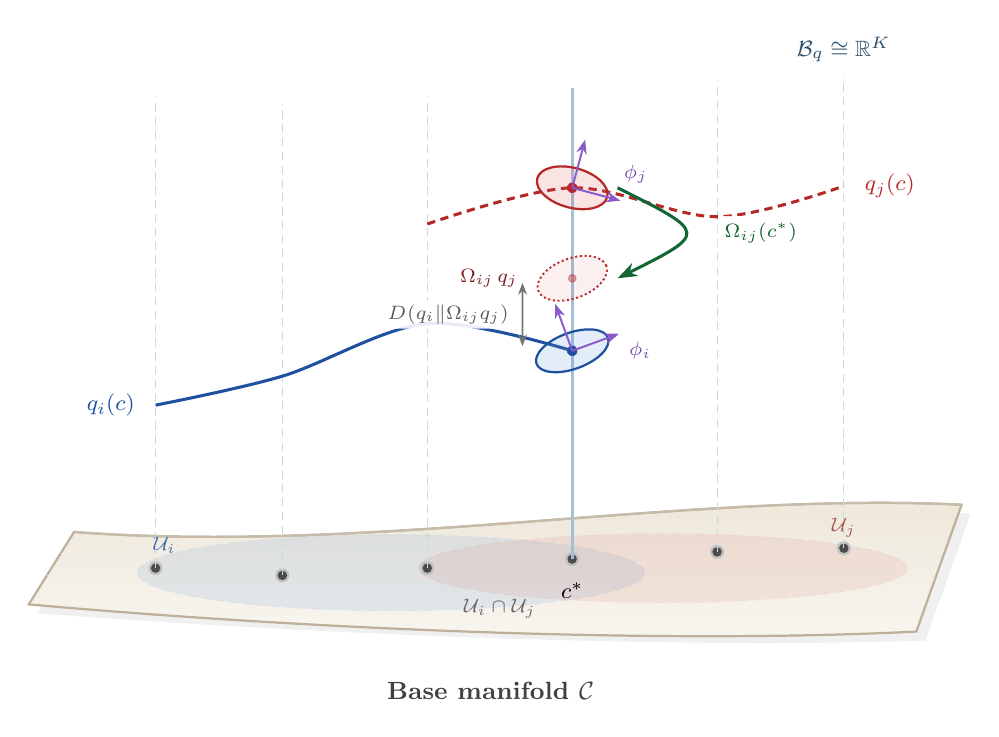
\begin{tikzpicture}[scale=1.15, every node/.style={font=\small}]

% =====================================================================
% COLOR DEFINITIONS
% =====================================================================
\definecolor{fiberblue}{RGB}{70,130,180}
\definecolor{sectionblue}{RGB}{30,80,160}
\definecolor{sectionred}{RGB}{180,40,40}
\definecolor{transportgreen}{RGB}{20,120,60}
\definecolor{gaussblue}{RGB}{100,150,220}
\definecolor{gaussred}{RGB}{220,100,100}
\definecolor{framecol}{RGB}{140,90,200}
\definecolor{basetan}{RGB}{230,220,200}
\definecolor{baseedge}{RGB}{160,140,110}
\definecolor{neighborblue}{RGB}{80,140,210}
\definecolor{neighborred}{RGB}{210,110,100}

% =====================================================================
% BASE MANIFOLD — gently curved surface
% =====================================================================
\path
  (-0.3,0.1) coordinate (M1)
  (9.5,0.4) coordinate (M2)
  (9.0,-1.0) coordinate (M3)
  (-0.8,-0.7) coordinate (M4);

% Shadow
\filldraw[fill=black!6, draw=none]
  ($(M1)+(0.1,-0.1)$)
    .. controls (3.0,-0.2) and (6.5,0.6) .. ($(M2)+(0.1,-0.1)$)
    -- ($(M3)+(0.1,-0.1)$)
    .. controls (6.0,-1.2) and (2.0,-1.0) .. ($(M4)+(0.1,-0.1)$)
    -- cycle;

% Surface fill
\shade[top color=basetan!70, bottom color=basetan!25, draw=baseedge!70, thick]
  (M1)
    .. controls (3.0,-0.15) and (6.5,0.55) .. (M2)
    -- (M3)
    .. controls (6.0,-1.15) and (2.0,-0.95) .. (M4)
    -- cycle;

% Front edge
\draw[baseedge!60, thick]
  (M1) .. controls (3.0,-0.15) and (6.5,0.55) .. (M2);

% Subtle grid lines for depth
\foreach \t in {0.3, 0.6} {
  \draw[baseedge!15, very thin]
    ($(M1)!\t!(M4)$) .. controls
    ($($(M1)!\t!(M4)$)!0.4!($(M2)!\t!(M3)$)+(0,0.04)$) and
    ($($(M1)!\t!(M4)$)!0.6!($(M2)!\t!(M3)$)+(-0.02,-0.04)$)
    .. ($(M2)!\t!(M3)$);
}

\node[below, black!75, font=\small\bfseries] at (4.3,-1.45) {Base manifold $\mathcal{C}$};

% =====================================================================
% FIBER ANCHOR POINTS — six points along the base surface
%
% Layout: C1, C2 in U_i only; C3, C4 in overlap U_i∩U_j;
%         C5, C6 in U_j only.
% =====================================================================
\coordinate (C1) at (0.6,-0.30);
\coordinate (C2) at (2.0,-0.38);
\coordinate (C3) at (3.6,-0.30);
\coordinate (C4) at (5.2,-0.20);
\coordinate (C5) at (6.8,-0.12);
\coordinate (C6) at (8.2,-0.08);

% =====================================================================
% LOCAL OPEN NEIGHBORHOODS U_i, U_j ON THE BASE — with overlap
%
% U_i covers C1–C4 (left through overlap).
% U_j covers C3–C6 (overlap through right).
% Overlap region contains C3, C4 — where both sections coexist.
% =====================================================================

% U_i: agent i's local open set (left to center)
% Center at x=3.0 with x-radius 3.0 → right edge at x=6.0, covering C4 at x=5.2
% y-radius 0.35 keeps the ellipse within the base surface (top edge ~y=0.0 here)
\filldraw[neighborblue, opacity=0.12, draw=neighborblue!60,
          line width=0.5pt, densely dashed]
  (3.2,-0.35) ellipse (2.8 and 0.42);
\node[neighborblue!80!black, font=\scriptsize] at (0.7,-0.05) {$\mathcal{U}_i$};

% U_j: agent j's local open set (center to right)
\filldraw[neighborred, opacity=0.12, draw=neighborred!60,
          line width=0.5pt, densely dashed]
  (6.2,-0.30) ellipse (2.7 and 0.38);
\node[neighborred!80!black, font=\scriptsize] at (8.2,0.15) {$\mathcal{U}_j$};

% Overlap label — between C3 and C4
\node[black!60, font=\scriptsize] at (4.4,-0.75) {$\mathcal{U}_i \cap \mathcal{U}_j$};

% Anchor dots
\foreach \c in {C1,C2,C3,C4,C5,C6} {
  \filldraw[black!25] (\c) circle (2pt);
  \filldraw[black!70] (\c) circle (1.3pt);
}

% =====================================================================
% FIBERS — vertical lines rising from each anchor
% =====================================================================
\pgfmathsetmacro{\fh}{5.2}

\foreach \c in {C1,C2,C3,C4,C5,C6} {
  \draw[fiberblue!30, densely dashed, line width=0.4pt]
    (\c) -- ++(0,\fh);
}

% Fiber label (rightmost)
\node[above=2pt, fiberblue!60!black, font=\footnotesize]
  at ($(C6)+(0,\fh)$) {$\mathcal{B}_q \cong \mathbb{R}^K$};

% =====================================================================
% SECTION CURVES — agents i and j as smooth sections of the bundle
%
% CRITICAL: Each section is defined only over its own neighborhood.
%   q_i(c) exists over U_i: fibers C1, C2, C3, C4 (blue section)
%   q_j(c) exists over U_j: fibers C3, C4, C5, C6 (red section)
% Both sections coexist at C3 and C4 (the overlap U_i ∩ U_j).
% =====================================================================

% --- Section q_i (blue, solid) — defined over U_i only (C1–C4) ---
\coordinate (Si1) at ($(C1)+(0,1.8)$);
\coordinate (Si2) at ($(C2)+(0,2.2)$);
\coordinate (Si3) at ($(C3)+(0,2.7)$);
\coordinate (Si4) at ($(C4)+(0,2.3)$);

\draw[sectionblue, line width=1.1pt]
  plot[smooth, tension=0.55] coordinates {
    (Si1) (Si2) (Si3) (Si4)
  };

% --- Section q_j (red, dashed) — defined over U_j only (C3–C6) ---
\coordinate (Sj3) at ($(C3)+(0,3.8)$);
\coordinate (Sj4) at ($(C4)+(0,4.1)$);
\coordinate (Sj5) at ($(C5)+(0,3.7)$);
\coordinate (Sj6) at ($(C6)+(0,4.0)$);

\draw[sectionred, densely dashed, line width=1.1pt]
  plot[smooth, tension=0.55] coordinates {
    (Sj3) (Sj4) (Sj5) (Sj6)
  };

% Section labels — each at the end within its own neighborhood
\node[sectionblue, font=\footnotesize, left=4pt] at (Si1) {$q_i(c)$};
\node[sectionred, font=\footnotesize, right=4pt] at (Sj6) {$q_j(c)$};

% =====================================================================
% HIGHLIGHT FIBER AT c* — at C4, solidly in the overlap U_i ∩ U_j
%
% At this single point c*, BOTH sections q_i(c*) and q_j(c*) live
% in the SAME fiber. The transport Ω_ij(c*) acts WITHIN this fiber
% to align j's frame to i's frame. c* lies in U_i ∩ U_j.
% =====================================================================

% Highlight the fiber at c*
\draw[fiberblue!50, line width=1.0pt] (C4) -- ++(0,\fh);

% Label c* on the base
\node[below=5pt, black, font=\footnotesize\itshape] at (C4) {$c^*$};

% --- Gaussian ellipses at c* showing beliefs in the SAME fiber ---

% q_i(c*): blue Gaussian, frame tilted 20°
\begin{scope}[shift={(Si4)}, rotate=20]
  \filldraw[gaussblue, opacity=0.18] (0,0) ellipse (0.42 and 0.20);
  \draw[sectionblue, line width=0.8pt] (0,0) ellipse (0.42 and 0.20);
  \filldraw[sectionblue] (0,0) circle (1.5pt);
\end{scope}

% q_j(c*): red Gaussian, frame tilted -15° (different gauge frame)
\begin{scope}[shift={(Sj4)}, rotate=-15]
  \filldraw[gaussred, opacity=0.18] (0,0) ellipse (0.40 and 0.22);
  \draw[sectionred, line width=0.8pt] (0,0) ellipse (0.40 and 0.22);
  \filldraw[sectionred] (0,0) circle (1.5pt);
\end{scope}

% --- Local gauge frames at c* (purple axes) ---

% Frame for agent i at c*
\begin{scope}[shift={(Si4)}, rotate=20]
  \draw[-{Stealth[length=1.8mm]}, framecol, line width=0.7pt]
    (0,0) -- (0.55,0);
  \draw[-{Stealth[length=1.8mm]}, framecol, line width=0.7pt]
    (0,0) -- (0,0.55);
\end{scope}
\node[framecol!80!black, font=\scriptsize] at ($(Si4)+(0.75,0.0)$) {$\phi_i$};

% Frame for agent j at c*
\begin{scope}[shift={(Sj4)}, rotate=-15]
  \draw[-{Stealth[length=1.8mm]}, framecol, line width=0.7pt]
    (0,0) -- (0.55,0);
  \draw[-{Stealth[length=1.8mm]}, framecol, line width=0.7pt]
    (0,0) -- (0,0.55);
\end{scope}
\node[framecol!80!black, font=\scriptsize] at ($(Sj4)+(0.7,0.15)$) {$\phi_j$};

% =====================================================================
% GAUGE TRANSPORT Ω_ij — acts WITHIN the fiber over c*
%
% At c*, Ω_ij(c*) rotates q_j(c*) from j's local frame into i's
% local frame. Both distributions live in the same fiber; the
% transport is a frame change, not a spatial translation.
% =====================================================================

% Transported ghost: Ω_ij q_j shown near q_i (now in i's frame, dotted)
% Placed 0.8 above q_i, giving space between q_i and ghost
\coordinate (Ghost) at ($(Si4)+(0,0.8)$);
\begin{scope}[shift={(Ghost)}, rotate=20]
  \filldraw[gaussred, opacity=0.10] (0,0) ellipse (0.40 and 0.22);
  \draw[sectionred, densely dotted, line width=0.7pt] (0,0) ellipse (0.40 and 0.22);
  \filldraw[sectionred, opacity=0.4] (0,0) circle (1.2pt);
\end{scope}

% Ghost label — well to the LEFT to avoid green arrow on the right
\node[sectionred!70!black, font=\scriptsize,
      fill=white, fill opacity=0.9, text opacity=1,
      inner sep=1.5pt, rounded corners=1pt, anchor=east]
  at ($(Ghost)+(-0.55,0)$) {$\Omega_{ij}\,q_j$};

% Transport arrow: curved arc WITHIN the fiber on the RIGHT side,
% from q_j(c*) down to the ghost near q_i(c*).
% Pushed further right (1.4) to clear the ghost label and ellipse.
\draw[-{Stealth[length=2.5mm, width=1.8mm]},
      transportgreen!85!black, line width=1.1pt]
  ($(Sj4)+(0.5,0)$)
    .. controls ($(Sj4)+(1.5,-0.5)$) and ($(Ghost)+(1.5,0.5)$)
    .. ($(Ghost)+(0.5,0)$);

% Transport label — positioned to the right of the arc, well clear
\node[transportgreen!80!black, font=\scriptsize\bfseries,
      fill=white, fill opacity=0.9, text opacity=1,
      inner sep=2.5pt, rounded corners=2pt, anchor=west]
  at ($(Sj4)!0.5!(Ghost)+(1.6,0)$) {$\Omega_{ij}(c^*)$};

% =====================================================================
% KL DIVERGENCE — between q_i(c*) and transported Ω_ij q_j(c*)
% Both distributions are now expressed in agent i's frame
% within the same fiber over c*. Label on the LEFT side.
% =====================================================================

% Double arrow between q_i and the ghost (left side)
\draw[{Stealth[length=1.5mm]}-{Stealth[length=1.5mm]},
      black!55, line width=0.6pt]
  ($(Si4)+(-0.55,0.05)$) -- ($(Ghost)+(-0.55,-0.05)$);

\node[black!65, font=\scriptsize,
      fill=white, fill opacity=0.9, text opacity=1,
      inner sep=1.5pt, rounded corners=1pt, anchor=east]
  at ($(Si4)+(-0.65,0.40)$) {$D_{\KL}(q_i \| \Omega_{ij} q_j)$};

\end{tikzpicture}
\caption{%
Agent belief sections over the associated bundle
$\mathcal{E}_q = \mathcal{N} \times_{\rho_q} \mathcal{B}_q$.
The shaded surface is the base manifold $\mathcal{C}$;
vertical dashed lines are belief fibers $\mathcal{B}_q \cong \mathbb{R}^K$.
Agents $i$ and $j$ each have a local open neighborhood on $\mathcal{C}$:
$\mathcal{U}_i$ (blue, dashed) and $\mathcal{U}_j$ (red, dashed).
Each agent's section is defined only over its own neighborhood:
the blue section $q_i(c)$ exists over $\mathcal{U}_i$,
the red section $q_j(c)$ over $\mathcal{U}_j$.
In the overlap $\mathcal{U}_i \cap \mathcal{U}_j$,
both sections coexist in the same fibers.
At the highlighted fiber over $c^* \in \mathcal{U}_i \cap \mathcal{U}_j$,
$q_i(c^*)$ and $q_j(c^*)$ reside in the same fiber
but are expressed in different local gauge frames
$\phi_i$, $\phi_j$ (purple axes).
The transport operator
$\Omega_{ij}(c^*) = \exp(\phi_i)\exp(-\phi_j)$
(green arrow) acts within this fiber,
rotating $q_j$ from $j$'s frame into $i$'s frame
to produce $\Omega_{ij}\,q_j$ (dotted red ellipse).
The attention cost $D_{\mathrm{KL}}(q_i \| \Omega_{ij}\,q_j)$
is then the divergence between same-frame distributions within a single fiber.
For transformers ($\dim\mathcal{C} = 0$),
all tokens share one base point, the neighborhoods collapse to a single point,
and the entire computation occurs within one fiber.
}
\label{fig:bundle_sections_surface}
\end{figure}

\subsection{The Base Manifold: Noumenal Space}

Agents form beliefs about something. We call this underlying domain the base manifold $\mathcal{C}$, following Kant's distinction between phenomena (appearances to observers) and noumena (things-in-themselves). The base manifold represents what agents are trying to understand, not how they understand it.

\begin{definition}[Base Manifold]
The base space $\mathcal{C}$ is a smooth $n$-dimensional manifold representing the noumenal substrate over which agents maintain probability distributions.
\end{definition}

\textbf{Conceptual point:} $\mathcal{C}$ is not physical spacetime. Physical space and time will emerge as induced structures when agents pull back metrics from their belief fields (Section~\ref{sec:pullback}). The base manifold is logically prior to spacetime - it's the abstract domain of inquiry upon which informational structure will be built.

For concreteness, consider several examples. In physics applications, $\mathcal{C}$ might be a configuration space $\mathbb{R}^n$ where agents maintain beliefs about particle positions. In directional sensing, $\mathcal{C} = S^2$ represents spherical directions about which agents have probabilistic beliefs. In language modeling (Section~\ref{sec:transformers}), $\mathcal{C}$ can be discrete - a sequence of token positions - with agents maintaining beliefs about vocabulary distributions at each position.

We use local coordinates $c = (c^1, \ldots, c^n)$ on $\mathcal{C}$, though the manifold structure exists independently of coordinate choice.

\subsection{Statistical Manifolds: Beliefs and Models}
\label{sec:statistical_manifolds}

At each point $c \in \mathcal{C}$, agents maintain probability distributions on two information-geometric arenas. The first holds distributions over the latent state $k$ that an agent is trying to infer; the second holds distributions over the parameters $m$ of the agent's generative model. Beliefs and the priors that anchor them live on the first arena, while generative models and their hyper-priors live on the second. These four statistical fields are organized into a fast subsystem $(q_i, p_i)$ that updates on the perceptual timescale and a slow subsystem $(s_i, r_i)$ that updates on the learning timescale, with the priors and hyper-priors interpreted not as independent dynamical variables but as the cross-scale shadows of the beliefs and models at the meta-agent scale immediately above (Section~\ref{sec:participatory}).

\begin{definition}[Statistical Manifolds]
Let $\mathcal{B}_{\mathrm{state}}$ denote the manifold of probability distributions over the latent state $k \in \mathbb{R}^K$, and let $\mathcal{B}_{\mathrm{model}}$ denote the manifold of probability distributions over generative-model parameters $m \in \mathbb{R}^M$. Each is equipped with the Fisher-Rao metric:
\begin{equation}
g_{\mathcal{B}}(\partial_a, \partial_b) = \mathbb{E}\left[(\partial_a \log \rho)(\partial_b \log \rho)\right],
\end{equation}
defining distances between distributions on the corresponding sample space (with $\rho$ standing for the relevant density and indices $a, b$ ranging over coordinates on the manifold).
\end{definition}

Beliefs $q_i$ and priors $p_i$ both take values in $\mathcal{B}_{\mathrm{state}}$, while generative models $s_i$ and hyper-priors $r_i$ both take values in $\mathcal{B}_{\mathrm{model}}$. The two manifolds are generically distinct because the latent state $k$ and the model parameters $m$ are different objects with different sample spaces, and may have different dimensions.

The Fisher-Rao metric provides natural Riemannian geometry on probability spaces. It measures how distinguishable nearby distributions are statistically: distributions with sharper peaks (higher information content) are further apart. The metric is unique up to scaling as the only Riemannian metric on probability spaces invariant under sufficient statistics~\cite{Cencov1982}.

Throughout this work, both arenas are realized concretely as Gaussian families:
\begin{equation}
\mathcal{B}_{\mathrm{state}} = \{\mathcal{N}(\mu, \Sigma) : \mu \in \mathbb{R}^K, \Sigma \succ 0\},
\qquad
\mathcal{B}_{\mathrm{model}} = \{\mathcal{N}(\mu, \Sigma) : \mu \in \mathbb{R}^M, \Sigma \succ 0\},
\end{equation}
the spaces of $K$- and $M$-dimensional multivariate Gaussian distributions, parametrized by mean vectors and positive-definite covariance matrices and forming $(K + K(K+1)/2)$- and $(M + M(M+1)/2)$-dimensional manifolds respectively.

The Fisher-Rao metric naturally induces several information-theoretic quantities. The Kullback-Leibler divergence between two distributions $q$ and $p$ on the same manifold measures their relative entropy

\begin{equation}
\mathrm{KL}(q \| p) = \int q(x) \log\frac{q(x)}{p(x)} dx \geq 0.
\end{equation}

This divergence is not symmetric ($\mathrm{KL}(q \| p) \neq \mathrm{KL}(p \| q)$) but it generates the Fisher metric through its Hessian structure. The natural gradient $\tilde{\nabla}_q f = g^{-1}_{\mathcal{B}} \nabla_q f$ provides the steepest descent direction in the curved probability space.

For Gaussian distributions specifically, the KL divergence has closed form:
\begin{equation}
\mathrm{KL}(\mathcal{N}(\mu_1, \Sigma_1) \| \mathcal{N}(\mu_2, \Sigma_2)) = \frac{1}{2}\left[\log\frac{|\Sigma_2|}{|\Sigma_1|} + \mathrm{tr}(\Sigma_2^{-1}\Sigma_1) + (\mu_2 - \mu_1)^\top\Sigma_2^{-1}(\mu_2 - \mu_1) - K\right]
\label{eq:gaussian_kl}
\end{equation}

This formula will be used extensively for computing belief and prior alignment terms.

\paragraph{Priors and hyper-priors as cross-scale shadows.}
A central economy of the framework is that the prior $p_i^{(s)}$ and the hyper-prior $r_i^{(s)}$ at scale $s$ are not independent dynamical fields but are determined by top-down transport from the meta-agent that envelopes agent $i$ at scale $s+1$. Concretely,
\begin{equation}
p_i^{(s)}(c) = \Omega_{i,I}\big[q_I^{(s+1)}\big](c),
\qquad
r_i^{(s)}(c) = \tilde\Omega_{i,I}\big[s_I^{(s+1)}\big](c),
\label{eq:cross_scale_shadow}
\end{equation}
where $I$ indexes the meta-agent at scale $s+1$ that contains agent $i$ as a constituent, $\Omega_{i,I}$ is the gauge-covariant transport into agent $i$'s frame on the latent-state fiber, and $\tilde\Omega_{i,I}$ is its model-fiber counterpart. The fast-channel relation is the formal content of the participatory feedback equation at Eq.~\eqref{eq:topdown_priors}; the slow-channel relation is its model-channel mirror. As a consequence, $p$ and $q$ live on the same statistical manifold $\mathcal{B}_{\mathrm{state}}$ (so the matched-bundle property of Section~\ref{sec:working_framework} is a theorem rather than a simplifying assumption), and $r$ and $s$ live on the same manifold $\mathcal{B}_{\mathrm{model}}$. The hierarchy $r \to s \to p \to q \to \text{observations}$ posited at the agent definition below is therefore realized cross-scale: $r$ regularizes $s$ because $r$ is the meta-agent's model transported down, and $p$ regularizes $q$ because $p$ is the meta-agent's belief transported down.

The hierarchy bottoms out at two boundaries. At the top scale ($s = s_{\max}$) there is no enveloping meta-agent, so the hyper-prior $r_i^{(s_{\max})}$ is treated as a fixed boundary condition encoding evolutionary or training-time structural defaults, and the top-scale prior is set self-referentially by aggregating across all active agents (Section~\ref{sec:participatory}). At the bottom scale ($s = 0$) the system has no constituents below it, so cross-scale propagation acts only downward from above. In the empirical simulations of Section~\ref{sec:meta_agent_emergence} all agents reside at a single scale and $p_i, r_i$ are treated as primitive boundary conditions with no super-agent above; the multi-scale relation~\eqref{eq:cross_scale_shadow} becomes operative only in the participatory dynamics of Section~\ref{sec:participatory}.

\subsection{Principal Bundles and Gauge Freedom}
\label{sec:agents_as_sections}

We now address the third challenge: different agents use different internal (cognitive) reference frames when representing beliefs and models. A physicist measuring particle spin uses basis vectors in their laboratory frame. Another physicist with a rotated laboratory measures the same physics but obtains different numerical values. Both descriptions are equally valid - they're related by transformations.

More generally, agents maintain beliefs using internal coordinate systems, conceptual frameworks, or measurement conventions: their gauge frames. These frames are necessary for representing probabilistic information, and the framework employs them in two distinct roles that the reader must keep separate.

\paragraph{Two roles for the gauge frame.} The same symbol $\phi_i$ does double duty in this manuscript, and conflating the two roles is the source of several apparent contradictions. In its \emph{transport role} (Role A), the frame is gauge-redundant: any pair of frame fields $\phi_i, \phi_j$ enters the dynamics only through the relative transport $\Omega_{ij} = U_iU_j^{-1}$, which is invariant under simultaneous right-translation $U_i \mapsto U_i g$ for all agents (Section~\ref{sec:transport}). Observable consequences of the transport structure depend only on the orbit of the frame collection under this global gauge action; an isolated frame carries no physical content. This is the redundancy reading the manuscript invokes when it speaks of "arbitrary frames" or "gauge invariance" of observables. In its \emph{state role} (Role B), the per-agent frame is treated as an internal cognitive state variable that contributes to ontology: distinct agent frames generate distinct frame-dependent pulled-back geometries $G_i^{(q)}$ (Section~\ref{sec:pullback}), distinct phenomenal characters in the qualia discussion (Section~\ref{sec:qualia}), and distinct signature mechanisms in the worked example of Section~\ref{sec:signature_resolution}. Quantities computed in Role B (such as $G_i^{(q)}$ or $\mathrm{tr}(A^{(i)}_\mu A^{(i)}_\nu)$) are gauge-covariant rather than gauge-invariant: they transform under $U_i \mapsto U_i g$ rather than remaining fixed. The framework makes both roles available without identifying the frame in Role B with mere description; any sentence that calls the frame "pure gauge" or "arbitrary" is invoking Role A, while any sentence in which the frame contributes to phenomenology, signature, or ontology is invoking Role B. Gauge-invariant observables of the framework are recovered from Role-B quantities by averaging over the gauge orbit (Section~\ref{sec:consensus_metric}); when no such average is taken, what is computed is a frame-dependent quantity, and we say so.

In what follows, the words "gauge-invariant" and "gauge-covariant" are reserved for their standard mathematical meanings: invariant means unchanged under the simultaneous right-translation, covariant means transforming according to a fixed representation. We use "frame-dependent" rather than "gauge-dependent" when referring to Role-B quantities, to signal that the dependence is on the cognitive state $\phi_i$ rather than on a redundant labelling.

\paragraph{Why the dual role is mathematically rigorous.}
\label{sec:dual_role_rigor}
The simultaneous Role-A / Role-B treatment of $\phi_i$ is not an ad hoc convenience; it is the discrete analog of three well-developed mechanisms in modern gauge theory and quantum reference frames. Edge modes in gauge theory~\cite{DonnellyFreidel2016} promote ``would-be pure-gauge'' boundary data to genuine physical degrees of freedom whenever a region's interior is treated as a subsystem: the boundary modes are gauge-redundant from the global standpoint but carry physical, symplectically conjugate information at the boundary of the subsystem. Quantum reference frames~\cite{BartlettRudolphSpekkens2007,Vanrietvelde2020} formalise this for finite quantum systems: a reference frame is gauge from a global perspective-neutral viewpoint, but is a physical system carrying state from its own perspective and from that of any other system relative to which it is described. Rovelli's relational interpretation~\cite{Rovelli1996}, already cited as the closest physics-side antecedent, sits in the same family: properties have meaning only relative to other systems, and ``the same data'' is gauge or physical depending on which slice of the relational structure one inspects. Each of these literatures argues, by independent routes, that a frame field can rigorously serve both roles when one is precise about which gauge subgroup is acting.

In the present framework, the bulk gauge action is the global diagonal right-translation $U_i \to U_i g$ for a single $g \in G$ shared across all agents; under this action $\phi_i$ is purely redundant and only $\Omega_{ij}$ is invariant, in agreement with Role~A. The agent-local frame data $\phi_i: \mathcal{U}_i \to \mathfrak{g}$ is the analog of edge-mode / quantum-reference-frame content: from the perspective of the network the choice of $\phi_i$ at a single agent specifies that agent's relational stance and is physical, in agreement with Role~B. Quantities like $\mathrm{tr}(A^{(i)}_\mu A^{(i)}_\nu)$ are not invariant under the full local gauge $g_i = g_i(c)$ that introduces a Maurer--Cartan derivative term, but are invariant under the constant-per-agent residual subgroup $\{(g_i)_{i \in I} : g_i \in G \text{ constant in } c\}$, since $\mathrm{tr}(g^{-1}A_\mu g \cdot g^{-1}A_\nu g) = \mathrm{tr}(A_\mu A_\nu)$ by trace cyclicity when $g$ is $c$-constant. The Lorentzian-signature mechanism, the pulled-back metric, and the gauge-curvature linguistic conjecture therefore live under this residual subgroup rather than under the full local gauge; we attach this restriction to each occurrence below rather than appealing to a uniformly stated invariance.

\begin{definition}[Principal Bundle]
Let $\pi: \mathcal{N} \to \mathcal{C}$ be a principal $G$-bundle where:
\begin{itemize}
\item $\mathcal{N}$ is the total space (all possible gauge choices at all base points)
\item $\mathcal{C}$ is the base manifold (the noumenal domain)
\item $G$ is the structure group (typically $G = \mathrm{SO}(N)$) acting freely on the right on $\mathcal{N}$
\end{itemize}
The projection satisfies $\pi(n \cdot g) = \pi(n)$ for all $g \in G$, meaning group action preserves fibers.
\end{definition}

\paragraph{Local trivializations and the scope of the bundle formalism.}
\label{sec:local_trivialization}
A general principal $G$-bundle does not admit a global section: a globally defined Lie-algebra-valued frame field $\phi: \mathcal{C} \to \mathfrak{g}$ exists if and only if the bundle is trivializable, i.e., $\mathcal{N} \cong \mathcal{C} \times G$ as a $G$-space. The framework as constructed below operates exclusively in local trivializing patches $\{\mathcal{U}_i\}$ that cover $\mathcal{C}$, with each $\phi_i: \mathcal{U}_i \to \mathfrak{g}$ a local section of the trivialization restricted to agent~$i$'s domain of operation. On overlaps $\mathcal{U}_i \cap \mathcal{U}_j$, the transition function $\Omega_{ij} = U_iU_j^{-1}$ relates the two local trivializations and satisfies the standard \v{C}ech cocycle condition $\Omega_{ij}\Omega_{jk} = \Omega_{ik}$ on triple overlaps (Theorem~\ref{thm:vanishing_holonomy}). The cocycle is therefore the natural mathematical object of the framework; the global bundle $\mathcal{N}$ is the formal \v{C}ech limit of these patches, and any expression that appears to require a global section should be read as a patch-wise statement composed via the transition functions. The framework's nontrivial-holonomy extension (Section~\ref{sec:discrete_regime_ii}) is the lattice gauge promotion of the cocycle in which the transition functions acquire an independent edge-local connection $\delta_{ij}$ between vertex factors.

Two technical caveats accompany this restriction. First, the exponential parameterisation $U_i(c) = \exp[\phi_i(c)]$ is only locally bijective: the exponential map $\exp: \mathfrak{g} \to G$ is surjective for connected compact groups (such as the $G = \mathrm{SO}(N)$ used in the proof-of-concept simulations), but for the non-compact group $\mathrm{GL}^+(K)$ relevant to the natural variational-inference setting, a single $\phi$ does not parameterise every group element. This is handled either by restricting $\phi_i$ to a neighborhood of zero on which $\exp$ is bijective, or by passing to a polar/Cartan decomposition $U = \exp(X)\exp(Y)$ with two Lie-algebra elements (one symmetric, one antisymmetric) so that the full group is covered by two exponential charts; the framework's empirical work uses connected-compact $G = \mathrm{SO}(N)$, where the issue does not arise. Second, the Maurer--Cartan one-form $\theta = U^{-1}dU$ in Section~\ref{sec:connection_forms} below is well-defined on each local patch independently of whether the global bundle is trivializable; the patch-wise cocycle structure is what the framework actually requires, and references to ``the global frame field $\phi$'' in subsequent discussion should be read in the local-trivialization sense unless explicitly noted otherwise.

Intuitively, each point $c \in \mathcal{C}$ sits above a fiber $\pi^{-1}(c) \cong G$ consisting of all possible gauge choices at that location. Moving within a fiber corresponds to changing reference frame without changing which point of $\mathcal{C}$ we're considering. The group $G$ parametrizes these frame transformations - for $G = \mathrm{SO}(3)$, these are rotations of internal coordinate axes.

This abstraction captures gauge freedom in physics (electromagnetic gauge transformations, coordinate changes in general relativity) but applies more broadly to any setting where agents must choose conventions for representing information. A cognitive agent's gauge frame might encode perceptual reference axes, categorical schemes, or other aspects of subjective framing.

The natural gauge group for KL-based variational inference on multivariate Gaussians is $G = \mathrm{GL}(K)$, with the proof-of-concept simulations in this work restricted to the compact subgroup $G = \mathrm{SO}(3)$ for computational tractability and visualizability. The full justification of this choice, including the formal $\mathrm{GL}(K)$ invariance theorem and the worked example in $\mathrm{GL}(K, \mathbb{C})$ that bears on the Lorentzian signature problem (Section~\ref{sec:signature_resolution}), is given in Section~\ref{sec:gauge_group_choice}.

\subsection{Associated Bundles: Attaching Probability Distributions to Gauge Structure}

Having established gauge structure through the principal bundle, we attach the two statistical manifolds $\mathcal{B}_{\mathrm{state}}$ and $\mathcal{B}_{\mathrm{model}}$ in a way that respects gauge transformations. This is accomplished through associated bundles, a standard construction in differential geometry~\cite{Nakahara2003,Frankel2011}.

The construction is as follows: if we change gauge frame (move within a fiber of $\mathcal{N}$), the probability distributions must transform accordingly. This requires specifying how the gauge group $G$ acts on each statistical manifold.

\begin{definition}[Representations and Associated Bundles]
Let $\rho_{\mathrm{state}}: G \to \mathrm{Aut}(\mathcal{B}_{\mathrm{state}})$ and $\rho_{\mathrm{model}}: G \to \mathrm{Aut}(\mathcal{B}_{\mathrm{model}})$ be smooth representations of $G$ on the two statistical manifolds. The associated bundles are
\begin{align}
\mathcal{E}_{\mathrm{state}} &:= \mathcal{N} \times_{\rho_{\mathrm{state}}} \mathcal{B}_{\mathrm{state}} \\
\mathcal{E}_{\mathrm{model}} &:= \mathcal{N} \times_{\rho_{\mathrm{model}}} \mathcal{B}_{\mathrm{model}}
\end{align}
where the equivalence relation $(n \cdot g, b) \sim (n, \rho(g)b)$ identifies gauge-transformed pairs and the appropriate $\rho$ is determined by which manifold $b$ inhabits.
\end{definition}

For Gaussian distributions with $G = \mathrm{GL}(K)$ (or any subgroup such as $\mathrm{SO}(N)$), the representation acts by linear transformation of means and congruence of covariances:
\begin{equation}
\rho_{\mathrm{state}}(g) \cdot \mathcal{N}(\mu, \Sigma) = \mathcal{N}(g\mu, g\Sigma g^\top),
\end{equation}
and analogously for $\rho_{\mathrm{model}}$ acting on the model-parameter fiber. This ensures that changing reference frame transforms probability distributions consistently. When $g \in \mathrm{SO}(N)$, this reduces to rotation; for general $g \in \mathrm{GL}(K)$, it includes scaling, shearing, and reflection. The associated bundles $\mathcal{E}_{\mathrm{state}}$ and $\mathcal{E}_{\mathrm{model}}$ are fiber bundles over $\mathcal{C}$ with fibers isomorphic to $\mathcal{B}_{\mathrm{state}}$ and $\mathcal{B}_{\mathrm{model}}$ respectively, and the four agent fields $(q_i, p_i)$ and $(s_i, r_i)$ are sections of these two bundles, with the prior and hyper-prior derived from the meta-scale via Eq.~\eqref{eq:cross_scale_shadow}.

\subsection{Agents as Smooth Sections}
\label{sec:agent_definition}

We can now define agents precisely as smooth sections of these associated bundles.

\begin{definition}[Agent]
An agent $\mathcal{A}^i$ at scale $s$ with support domain $\mathcal{U}_i \subseteq \mathcal{C}$ consists of two primitive smooth sections together with two derived sections and a gauge-frame field:
\begin{align}
q_i &: \mathcal{U}_i \to \mathcal{E}_{\mathrm{state}}|_{\mathcal{U}_i}, &&\text{(belief, primitive)} \\
s_i &: \mathcal{U}_i \to \mathcal{E}_{\mathrm{model}}|_{\mathcal{U}_i}, &&\text{(generative model, primitive)} \\
p_i &= \Omega_{i,I}\big[q_I^{(s+1)}\big] \in \Gamma\!\left(\mathcal{E}_{\mathrm{state}}|_{\mathcal{U}_i}\right), &&\text{(prior, derived)} \\
r_i &= \tilde\Omega_{i,I}\big[s_I^{(s+1)}\big] \in \Gamma\!\left(\mathcal{E}_{\mathrm{model}}|_{\mathcal{U}_i}\right), &&\text{(hyper-prior, derived)} \\
\phi_i &: \mathcal{U}_i \to \mathfrak{g}, &&\text{(gauge frame field)}
\end{align}
where $\mathfrak{g} = \mathrm{Lie}(G)$ is the Lie algebra of the gauge group and $I$ indexes the level-$(s{+}1)$ meta-agent that envelopes agent $i$ as a constituent. The four statistical sections are organized as the variational hierarchy
\[
r_i \to s_i \to p_i \to q_i \to \text{observations},
\]
realized cross-scale via Eq.~\eqref{eq:cross_scale_shadow}: $r_i^{(s)}$ regularizes $s_i^{(s)}$ because $r_i^{(s)}$ is the meta-agent's generative model transported down, and $p_i^{(s)}$ regularizes $q_i^{(s)}$ because $p_i^{(s)}$ is the meta-agent's belief transported down. At the top scale, $r_i^{(s_{\max})}$ becomes a fixed boundary condition encoding evolutionary or training-time defaults; at the bottom scale, the cross-scale relations act only downward. We follow the convention of the gauge-theoretic transformer companion paper~\cite{Dennis2025trans}: in the empirical simulations of this paper the slow subsystem $(s_i, r_i)$ is held fixed (model coupling $\gamma_{ij} = 0$) and only the fast subsystem $(q_i, p_i)$ is updated, with $p_i$ realized concretely by the per-token PriorBank (Section~\ref{sec:transformers}). The slow subsystem is retained in the free energy because it is required for the meta-agent / Ouroboros dynamics of Section~\ref{sec:participatory}, where consensus on generative models is the conceptual content of the $\gamma_{ij}\mathrm{KL}(s_i\|\tilde{\Omega}_{ij}s_j)$ term.
\end{definition}

The notation requires unpacking. Each agent maintains smooth probability distributions $q_i(c)$ and $p_i(c)$ at every point $c$ in their domain of operation $\mathcal{U}_i$. These are not single distributions but entire fields - functions mapping base manifold points to probability distributions. The gauge frame $\phi_i(c) \in \mathfrak{g}$ specifies which reference frame the agent uses at location $c$, encoded as a Lie algebra element generating local gauge transformations.

For Gaussian agents, this specializes to:
\begin{align}
q_i(c) &= \mathcal{N}(\mu_i(c), \Sigma_i(c)) \\
p_i(c) &= \mathcal{N}(\mu_i^p(c), \Sigma_i^p(c)) \\
s_i(c) &= \mathcal{N}(\mu_i^s(c), \Sigma_i^s(c)) \\
r_i(c) &= \mathcal{N}(\mu_i^r(c), \Sigma_i^r(c)) \\
\phi_i(c) &= \phi_i^a(c) G_a
\end{align}

where $\mu_i, \mu_i^p: \mathcal{U}_i \to \mathbb{R}^K$ are means on the latent-state fiber $\mathcal{B}_{\mathrm{state}}$ with $\Sigma_i, \Sigma_i^p \in \mathbb{S}^K_{++}$, while $\mu_i^s, \mu_i^r: \mathcal{U}_i \to \mathbb{R}^M$ are means on the model-parameter fiber $\mathcal{B}_{\mathrm{model}}$ with $\Sigma_i^s, \Sigma_i^r \in \mathbb{S}^M_{++}$. The pair $(\mu_i^p, \Sigma_i^p)$ is determined by Eq.~\eqref{eq:cross_scale_shadow} from the level-$(s{+}1)$ meta-agent's belief, and $(\mu_i^r, \Sigma_i^r)$ analogously from the meta-agent's generative model. The fields $\phi_i^a(c)$ are scalar coefficients, and $\{G_a\}$ are basis generators of the Lie algebra $\mathfrak{g}$ (specialized to $\mathfrak{so}(N)$ in the proof-of-concept simulations).

This formulation provides complete flexibility. Agents can maintain different beliefs at different locations (spatial variation in $q_i(c)$). They can use different reference frames at different locations (spatially varying gauge $\phi_i(c)$). Multiple agents can overlap spatially, each maintaining their own beliefs about the same region of $\mathcal{C}$. This generality will prove essential for modeling everything from transformer attention mechanisms to multi-agent coordination to emergent spacetime structure.

The framework is now mathematically complete: we have base manifold, statistical fibers, gauge structure, and agents as sections. The next step is introducing dynamics through variational free energy minimization.

\subsection{Multi-Agent Systems and Overlapping Perspectives}

\subsubsection{The Multi-Agent Configuration}

Reality in this framework emerges not from a single observer but from collective dynamics of multiple agents maintaining overlapping beliefs about the same underlying noumenal substrate. This multiplicity is essential - a single agent alone cannot generate the intersubjective structure we recognize as objective reality.

\begin{definition}[Multi-Agent System]
A multi-agent system $\mathcal{M}$ over base manifold $\mathcal{C}$ consists of a finite collection of agents:
\begin{equation}
\mathcal{M} = \left\{\mathcal{A}^i = (q_i, p_i, s_i, r_i, \phi_i)\right\}_{i \in \mathcal{I}},
\end{equation}
where $\mathcal{I}$ is an index set (typically $\mathcal{I} = \{1, 2, \ldots, N\}$), and each agent $\mathcal{A}^i$ operates over domain $\mathcal{U}_i \subseteq \mathcal{C}$. When the slow subsystem is held fixed, as in the simulations below, an agent is referred to by the abbreviated tuple $(q_i, p_i, \phi_i)$ without ambiguity.
\end{definition}

The domains $\mathcal{U}_i$ generally overlap, with $\mathcal{U}_i \cap \mathcal{U}_j \neq \emptyset$ for many agent pairs. This overlap is not incidental but fundamental - agents must share common ground to exchange information and coordinate beliefs. The intersection $\mathcal{U}_i \cap \mathcal{U}_j$ represents the region where both agents maintain explicit beliefs, enabling comparison and information exchange despite their potentially different gauge frames.

Each agent represents an autonomous information-processing entity with its own beliefs, priors, and reference frame. The domain $\mathcal{U}_i$ delineates the region of $\mathcal{C}$ about which agent $i$ maintains representations. In physical contexts, this might correspond to sensory range - a human observer can only form beliefs about the spatial region accessible to their senses. In cognitive contexts, different brain modules might process overlapping aspects of sensory input, each maintaining beliefs over partially overlapping representational spaces. In social contexts, communities maintain beliefs over shared cultural knowledge, with overlaps representing common ground for communication. In linguistic contexts, speakers maintain beliefs over semantic space, with overlaps representing shared meanings enabling successful communication.

\subsubsection{Consensus and Meta-Agent Formation}

When agents achieve sufficient alignment in their beliefs and models over shared regions, they can be understood as forming higher-order collective entities - meta-agents. This emergence of hierarchical structure from informational coherence constitutes one of the framework's central mechanisms.

\begin{definition}[Perfect Consensus]
Agents $\{i, j, \ldots\} \subseteq \mathcal{I}$ are in perfect consensus over region $\mathcal{R} \subseteq \bigcap_k \mathcal{U}_k$ if, after gauge transport to a common frame:
\begin{equation}
\Omega_{ij}[q_j](c) = q_i(c), \quad \tilde{\Omega}_{ij}[s_j](c) = s_i(c) \quad \forall c \in \mathcal{R},
\end{equation}
where $\Omega_{ij}$ is the gauge transport operator connecting their frames on the state fiber (see~\eqref{eq:transport_def}) and $\tilde{\Omega}_{ij}$ is the corresponding transport on the model fiber. Alignment of the cross-scale shadows $p_i, r_i$ follows automatically from belief and model consensus at the meta-scale via Eq.~\eqref{eq:cross_scale_shadow} and is not an independent condition.
\end{definition}

The gauge transport $\Omega_{ij}$ is essential here. Agents may describe the same beliefs using different internal coordinates (gauge frames), just as physicists in different laboratories describe the same spin state using rotated basis vectors. Perfect consensus means that after accounting for these frame differences through transport operations, the agents hold identical probabilistic beliefs and models about the shared region. They have achieved informational alignment despite maintaining distinct perspectives.

Perfect consensus is an idealization rarely achieved exactly. More realistically, agents achieve approximate consensus characterized by small KL divergences between transported beliefs. When this approximate consensus is sufficiently strong and stable across a cluster of agents, meta-agent formation becomes possible.

\begin{definition}[Meta-Agent]
A meta-agent $\mathcal{A}^{(s+1)}$ at hierarchical scale $(s+1)$ forms from a cluster $\{i, j, \ldots\} \subseteq \mathcal{I}^{(s)}$ of scale-$s$ agents satisfying: (1) sufficient coherence $C_{\text{belief}} \cdot C_{\text{model}} > \Gamma_{\min}$ above some threshold, (2) overlapping support $\bigcap_k \mathcal{U}_k \neq \emptyset$, and (3) minimum cluster size $|\{i, j, \ldots\}| \geq N_{\min}$ (typically $N_{\min} = 2$). The meta-agent is itself a smooth section $(q^{(s+1)}, p^{(s+1)}, s^{(s+1)}, r^{(s+1)}, \phi^{(s+1)})$ constructed via gauge-covariant averaging of constituent fields. Belief coherence $C_{\text{belief}}$ measures alignment of $q$-fields and model coherence $C_{\text{model}}$ measures alignment of $s$-fields, the latter being the substantive content of meta-cognitive consensus.
\end{definition}

Meta-agents represent emergent collective entities arising from coherent subsystems. A family forms a household meta-agent, neurons form brain modules, individuals form communities, communities form societies. meta-agents are not mere abstractions or statistical summaries. They are dynamical agents in their own right with beliefs evolving according to the same free energy minimization principles governing base agents. The meta-agent can influence its constituents through top-down feedback, realizing Wheeler's participatory loop where higher-level structure affects lower-level dynamics.

The construction of meta-agent beliefs from constituent beliefs requires careful gauge-covariant averaging procedures detailed in Section~\ref{sec:participatory}. Naively averaging beliefs from agents in different gauge frames produces meaningless results - we must first transport all beliefs to a common frame, compute the average, then assign an appropriate gauge frame to the resulting meta-agent. This ensures the meta-agent's beliefs remain well-defined geometric objects on the statistical manifold.

\subsubsection{Epistemic Collapse and Information Death}
\label{sec:epistemic_collapse}

The flip side of consensus formation is epistemic collapse - the pathological limit where agents become informationally indistinguishable, eliminating the diversity necessary for meaningful information exchange.

\begin{definition}[Epistemic Death]
A set of agents $\{i, j, \ldots\}$ is epistemically dead if their beliefs and generative models are completely aligned under gauge transport on both timescale channels:
\begin{align}
\mathrm{KL}(q_i(c) \| \Omega_{ij}[q_j](c)) &= 0 \\
\mathrm{KL}(s_i(c) \| \tilde{\Omega}_{ij}[s_j](c)) &= 0
\end{align}
for all $c \in \mathcal{U}_i \cap \mathcal{U}_j$ and all pairs $(i,j)$. The two conditions correspond, respectively, to the vanishing of the fast-channel coupling term $\beta_{ij}\mathrm{KL}(q_i \| \Omega_{ij}q_j)$ and the slow-channel coupling term $\gamma_{ij}\mathrm{KL}(s_i \| \tilde{\Omega}_{ij}s_j)$ in the canonical free energy. Alignment of priors $p_i$ and hyper-priors $r_i$ follows as a corollary: by the cross-scale shadow relation~\eqref{eq:cross_scale_shadow}, $p_i^{(s)}$ and $r_i^{(s)}$ are determined by the meta-agent's belief and generative model at scale $s+1$, so once the constituent beliefs and models collapse to common values up to gauge transport, the priors and hyper-priors are forced to match likewise.
\end{definition}

\begin{remark}
Epistemic death represents complete informational consensus, not geometric identity. Agents may maintain distinct gauge frames $\phi_i \neq \phi_j$ (different internal coordinates or perspectives) while agreeing perfectly on informational content after accounting for these perspective differences through the transport operators $\Omega_{ij}$ defined in~\eqref{eq:transport_def}.

In this state, no information gradients exist between agents, eliminating the driving force for learning or evolution. The free energy functional achieves a minimum with respect to inter-agent coupling terms. This is the informational analog of thermal equilibrium: maximum entropy configuration given constraints, with no further evolution possible.

Epistemic death is gauge-invariant. Under the simultaneous group-level transformation $U_i \mapsto U_i g$ for all agents (Section~\ref{sec:transport}), both KL conditions are preserved because $q_i$ and $\Omega_{ij}[q_j]$ transform identically (and likewise $s_i$ and $\tilde{\Omega}_{ij}[s_j]$ on the model fiber), so each KL is invariant. The Lie-algebra additive shorthand $\phi_i \mapsto \phi_i + \xi(c)$ realises this for abelian gauge groups or commuting $\xi$, with the full non-abelian invariance captured at the group level. This distinguishes epistemic death (informational equilibrium) from naive coordinate singularities (gauge-dependent artifacts).
\end{remark}

Epistemic death plays an important role in hierarchical emergence. When constituent agents of a meta-agent become epistemically dead, they can be integrated out and replaced by a single representative at the meta-level. This coarse-graining reduces degrees of freedom without information loss. The meta-agent effectively absorbs its constituents, becoming the complete description at higher scales. This enables efficient hierarchical modeling where complex multi-agent systems are described by simpler meta-agent representations.

However, epistemic death is neither inevitable nor desirable for the system as a whole. Even when agents form coherent meta-agents, they need not become completely epistemically dead. Agents may achieve consensus on some beliefs while maintaining diversity on others - agreeing about basic facts while disagreeing about interpretations. Different gauge frames preserve distinct perspectives even when beliefs align numerically. Top-down feedback from meta-agents may perturb constituents differently, actively maintaining diversity. New observations continuously introduce perturbations preventing complete collapse.

For a functioning participatory system, we require that agents not collapse into global epistemic death. Complete consensus across all agents would constitute the "heat death" of the informational universe - a static, non-participatory state where no further evolution occurs. The system would become frozen, with no information gradients to drive dynamics and no perspective diversity to generate new structure.

The framework must therefore maintain a delicate balance. Sufficient consensus enables meta-agent formation and hierarchical organization, providing stable structure. But sufficient diversity must persist to sustain information exchange, prevent complete collapse, and enable continued evolution. This tension between consensus-seeking and diversity-preservation drives perpetual dynamics in the participatory universe. Agents constantly negotiate between aligning with neighbors (reducing free energy through coordination) and maintaining individual perspectives (preserving information capacity for future observations).

This balance is maintained through several mechanisms. Observations from the noumenal substrate continuously perturb agent beliefs, introducing new information that breaks symmetry and prevents stagnation. Gauge freedom allows agents to maintain distinct perspectives even when beliefs converge - they can agree on content while disagreeing on framing. Hierarchical feedback creates heterogeneity as meta-agents influence constituents through different channels. Spatial separation limits coupling strength, preventing universal alignment. These mechanisms together ensure the system remains far from epistemic equilibrium, sustaining the participatory dynamics central to the framework's vision of reality as perpetually co-constructed through agent interactions.

\subsubsection{Hierarchical Structure and Cross-Scale Organization}

Meta-agents at scale $(s+1)$ can themselves cohere into meta-meta-agents at scale $(s+2)$, continuing upward to some maximum scale $s_{\max}$. This creates hierarchical architecture where individuals form groups, groups form communities, communities form societies, and so forth:
\begin{equation}
\text{Scale 0 (individuals)} \to \text{Scale 1 (groups)} \to \text{Scale 2 (communities)} \to \cdots \to s_{\max}.
\end{equation}

Information flows bidirectionally through this hierarchy. Bottom-up flow occurs through consensus formation and averaging - when agents at scale $s$ achieve coherence, their collective belief propagates upward to form scale $(s+1)$ meta-agent beliefs. Top-down flow occurs through prior propagation - meta-agents influence their constituents by providing high-level expectations that constrain lower-level beliefs. This bidirectional coupling realizes Wheeler's participatory loop: higher levels emerge from lower levels through coherence, then feed back to shape lower-level dynamics through expectation.

Each scale exhibits emergent properties absent at lower levels. Individual neurons fire stochastically, but neural assemblies exhibit stable attractor dynamics. Individual humans have limited knowledge, but scientific communities achieve collective understanding exceeding any individual. The whole exceeds the sum of its parts through information-geometric coupling.

the entire structure remains dynamical rather than static. Meta-agents do not simply form and freeze but continuously evolve as constituent beliefs shift. Feedback loops prevent equilibration - top-down expectations perturb constituents while bottom-up observations update meta-level beliefs. This perpetual dynamics sustains the participatory universe far from informational equilibrium. Section~\ref{sec:participatory} develops this multi-scale architecture rigorously, demonstrating computational validation of hierarchical emergence and sustained non-equilibrium operation.

\subsection{Cognitive Reference Frames as Gauge Frames}
\label{sec:cognitive_reference_frames}

\subsubsection{Cognitive Frames of Reference and the Need for an Explicit Transformation Law}

Lahav and Neemeh~\cite{LahavNeemeh2022,LahavNeemeh2025} argue that phenomenal consciousness is observer-relative the way simultaneity and velocity are observer-relative in special relativity: a cognitive system's experience is a property of that system viewed from its own cognitive frame of reference (CFR), not a fact independent of any observer. Their account asserts that there must therefore exist a transformation law relating quantities measured in one CFR to quantities measured in another, but does not write such a law down in its currently published form. The construction in this section supplies it. Each agent $i$ carries a smooth gauge frame field $\phi_i: \mathcal{U}_i \to \mathfrak{g}$ that plays the role of the agent's CFR; the transport operator $\Omega_{ij} = \exp(\phi_i)\exp(-\phi_j)$ defined immediately below is the transformation between CFRs; and the KL divergence $\mathrm{KL}(q_i \| \Omega_{ij}[q_j])$ is a frame-invariant scalar measuring belief disagreement after transport. Section~\ref{sec:lahav_convergence} develops this correspondence with the structural caveats it requires; one of them, that gauge invariance places no constraint on which gauge frame produces which phenomenal quale, is a real limitation of the identification and is registered there explicitly.

Once the cognitive-frames role is fixed, the formal analogue with general relativity is straightforward. Two physicists describing the same spacetime event in coordinates $(t, x, y, z)$ and $(t', x', y', z')$ relate their measurements via a coordinate transformation; two cognitive systems describing the same noumenal substrate in CFRs $\phi_i$ and $\phi_j$ relate their belief representations via $\Omega_{ij}$. The analogue is a working correspondence rather than an identity: the transformation group on the cognitive side is $\mathrm{GL}(K)$ (or, in the simulations here, the $\mathrm{SO}(N)$ subgroup), and the transformations act on probability distributions on a statistical manifold rather than on coordinates of a Lorentzian spacetime.

The gauge frame $\phi_i: \mathcal{U}_i \to \mathfrak{g}$ takes values in the Lie algebra of the structure group $G$ (typically $G = \mathrm{SO}(N)$ in our simulations, with $\mathrm{GL}(K)$ as the natural larger choice; see Section~\ref{sec:gauge_group_choice}). Intuitively, $\phi_i(c)$ specifies the agent's choice of internal axes for representing belief content at base point $c$; it is a field over the base manifold rather than a single matrix because the choice can vary spatially as the agent's representational requirements shift across the noumenal substrate; and it lives in $\mathfrak{g}$ because we want continuous deformations between nearby choices. For $G = \mathrm{SO}(3)$, an instance of $\phi_i$ is an internal rotation; for general $G$ it is a basis change in the agent's representational space, not an orientation in physical space.

A concrete example. Consider two agents perceiving the same coloured surface. Agent $i$ represents colour internally along an opponent-process basis with axes red--green and blue--yellow; agent $j$ represents colour along a different basis obtained by an internal linear change of axes. The agents agree about the underlying spectral content of the stimulus but disagree about the components in which they internally represent it. Their gauge frames $\phi_i(c)$ and $\phi_j(c)$ differ by the basis change that relates the two representational schemes, and their belief distributions $q_i$ and $q_j$ are accordingly expressed in different internal coordinate systems on the same fibre. Comparing their beliefs requires transport: $\Omega_{ij}[q_j]$ pushes agent $j$'s belief into agent $i$'s representational basis, after which the residual disagreement $\mathrm{KL}(q_i \|  \Omega_{ij}[q_j])$ is the part of the disagreement that does not reduce to a basis choice. The example with two agents facing different physical directions, reduced to a $90^\circ$ rotation about a vertical axis, is a special case of this construction in which the gauge group has been restricted to $\mathrm{SO}(3)$ acting on three-dimensional representations of body-centred axes, but it is not the general case Lahav and Neemeh have in mind, and we therefore lead with the perceptual example.

\subsubsection{Transport Operators: Translating Between Frames}
\label{sec:transport}

When agents $i$ and $j$ overlap at point $c \in \mathcal{U}_i \cap \mathcal{U}_j$, the inter-agent transport operator is defined as:
\begin{equation}
\Omega_{ij}(c) = \exp[\phi_i(c)] \exp[-\phi_j(c)] \in G.
\label{eq:transport_def}
\end{equation}

This group element transforms agent $j$'s representations into agent $i$'s frame. The transport operator acts on probability distributions through the representation $\rho: G \to \mathrm{Aut}(\mathcal{B})$, giving $\Omega_{ij}[q_j](c) := \rho(\Omega_{ij}(c))  q_j(c)$.

For Gaussian beliefs $q_j = \mathcal{N}(\mu_j, \Sigma_j)$ with $G = \mathrm{SO}(3)$, transport acts through rotation matrix $R_{ij} = \exp[\phi_i]\exp[ - \phi_j] \in \mathrm{SO}(3)$, transforming mean and covariance as $\mu_j \mapsto R_{ij} \mu_j$ and $\Sigma_j \mapsto R_{ij} \Sigma_j R_{ij}^\top$. The transported belief $\Omega_{ij}[q_j](c)$ represents "agent $j$'s belief at $c$, expressed in agent $i$'s coordinate system." This enables meaningful comparison - we can compute $\mathrm{KL}(q_i \| \Omega_{ij}[q_j])$ to measure belief discrepancy after accounting for frame differences.

\subsubsection{Gauge Covariance: The Fundamental Principle}

There are two distinct invariances at play here, and we want to keep them apart. The \emph{global diagonal redundancy} is a single right-translation $U_i \mapsto U_i g$ applied to all agents with the \emph{same} $g \in G$, under which $\Omega_{ij} = U_i U_j^{-1} \mapsto U_i g g^{-1} U_j^{-1} = \Omega_{ij}$ is invariant. This is the redundancy of the overall labelling of the gauge orbit and is the version we use throughout the body of this manuscript when we say "the framework is gauge-invariant." The \emph{full local gauge freedom} of a principal bundle is a stronger statement: independent right-translations $U_i \mapsto U_i g_i$ for each agent, with corresponding transformations of the transported quantities so that $\Omega_{ij} \mapsto g_i^{-1} \Omega_{ij} g_j$ and $q_j \mapsto \rho(g_j^{-1}) q_j$, under which $\Omega_{ij} q_j$ acquires $\rho(g_i^{-1})$ on the left and the pairwise KL $\mathrm{KL}(q_i \| \Omega_{ij} q_j)$ becomes invariant by KL invariance under common pushforward. The body construction is consistent with this stronger local invariance under the standard transformation laws, but we do not claim our central derivations exploit it; we use the global diagonal redundancy as the working notion of gauge invariance and flag the full local case where it matters.

The consequence of the global diagonal redundancy is that only relative gauge frames matter. Individual frames $\phi_i$ play two distinct roles in this manuscript -- a redundant labelling role (Role A) and a cognitive-state role (Role B), discussed in Section~\ref{sec:agents_as_sections} -- and we use ``gauge-invariant'' for quantities that are unchanged under both the global diagonal redundancy and the full local gauge action, while ``gauge-covariant'' is reserved for quantities that transform according to a specified representation. The Lie-algebra additive form $\phi_i \mapsto \phi_i + \xi$ coincides with the group-level form only when $\xi$ commutes with each $\phi_i$ (since the Baker-Campbell-Hausdorff expansion $\exp(\phi_i + \xi) = \exp(\phi_i)\exp(\xi)\exp(-\tfrac12 [\phi_i, \xi]) \cdots$ collapses to $\exp(\phi_i)\exp(\xi)$ only when the commutator vanishes), so the additive shift is the genuine gauge transformation only for abelian gauge groups or for $\xi$ in the centre. For the non-abelian groups used here, the group-level form $U_i \mapsto U_i g$ is the correct statement of gauge invariance. The relative pairing $U_i U_j^{-1}$ is gauge-invariant under the global diagonal action and gauge-covariant (transforming as $g_i^{-1}\Omega_{ij}g_j$) under independent agent-wise actions, in the same way that, in general relativity, individual coordinate systems are arbitrary while coordinate-invariant quantities like proper time are physically meaningful.

\subsubsection{Connection Forms and Parallel Transport}
\label{sec:connection_forms}

\paragraph{Two regimes for the gauge connection.} The framework admits two distinct regimes for the gauge connection, and the distinction matters for every subsequent claim about field strength, holonomy, and Yang-Mills structure. In \emph{Regime~I}, the connection is the pure-gauge object $A^{(i)}_\mu(c) = U_i^{-1}(c)\partial_\mu U_i(c)$ derived from the smooth agent frame $\phi_i$, the inter-agent transport $\Omega_{ij} = U_iU_j^{-1}$ is the cocycle of Theorem~\ref{thm:vanishing_holonomy}, and the curvature $F^{(i)}_{\mu\nu}$ vanishes identically (the Maurer--Cartan computation in Section~\ref{sec:gauge_transport_arbitrary} below). This regime is the one the present implementation realizes and the one the simulations of Sections~\ref{sec:participatory}--\ref{sec:transformers} compute. In \emph{Regime~II}, $A^{(i)}_\mu$ is promoted to an independent connection variable not constrained to factor as $U^{-1}dU$; transport along a path~$\gamma$ becomes the path-ordered exponential $\Omega_\gamma = \mathcal{P}\exp(-\int_\gamma A_\mu  dx^\mu)$ rather than a vertex-local product, and $F_{\mu\nu}$ becomes a genuine dynamical field with non-trivial holonomy. Several constructions in this manuscript -- Yang-Mills curvature regularizers, frame-twist holonomy, the Lorentzian-signature mechanism via $\mathrm{tr}(A_\mu A_\nu)$, and the gauge-curvature linguistic conjecture -- are formally meaningful only in Regime~II. We mark these passages as Regime~II content where they appear, and otherwise read the connection-form discussion below as developing the general gauge-theoretic vocabulary that becomes dynamically nontrivial only after the Regime~II promotion. A concrete discrete realization of Regime~II compatible with the agent-graph skeleton, which preserves the vertex-frame factors $U_i$ and admits non-trivial holonomy through an edge-local connection $\delta_{ij}$, is developed in Section~\ref{sec:discrete_regime_ii}.

The gauge frame $\phi_i$ induces a Lie-algebra-valued one-form on agent $i$'s domain,
\begin{equation}
\theta^{(i)}_\mu(c) := U_i^{-1}(c) \partial_\mu U_i(c) \in \mathfrak{g},
\label{eq:connection_form}
\end{equation}
where $U_i(c) = \exp[\phi_i(c)] \in G$ and $\partial_\mu = \partial/\partial c^\mu$. This is the (left) Maurer--Cartan frame-gradient pulled back along the agent's local section $U_i: \mathcal{U}_i \to G$ on the trivializing patch $\mathcal{U}_i$ (Section~\ref{sec:local_trivialization}), not a dynamical Yang-Mills connection: under the cocycle parameterisation $\Omega_{ij} = U_i U_j^{-1}$ the curvature $d\theta + \theta \wedge \theta$ vanishes identically (Section~\ref{sec:gauge_transport_arbitrary}). We retain the symbol $A^{(i)}_\mu$ for $\theta^{(i)}_\mu$ throughout the manuscript when the context is the frame-gradient reading; the Yang-Mills reading, in which $A$ is an independent connection variable, is the Regime~II extension introduced above.

On overlapping regions $\mathcal{U}_i \cap \mathcal{U}_j$, the relation between the two agents' frame-gradients follows from $U_i = \Omega_{ij} U_j$ and the chain rule:
\begin{equation}
\theta^{(i)}_\mu = \mathrm{Ad}(U_j^{-1})\big[\Omega_{ij}^{-1} \partial_\mu \Omega_{ij}\big] + \theta^{(j)}_\mu,
\label{eq:theta_overlap_relation}
\end{equation}
where $\mathrm{Ad}(U_j^{-1})$ denotes the adjoint action of $U_j^{-1}$ on $\mathfrak{g}$. Equation~\eqref{eq:theta_overlap_relation} is \emph{not} the standard Yang-Mills gauge-transformation law $A^{(i)} = g A^{(j)} g^{-1} - (dg) g^{-1}$, which holds for an independent connection variable under right-multiplication of the structure-group element. The mismatch reflects the fact that $\theta = U^{-1}dU$ is the pullback of a frame-gradient, not a section-independent gauge potential; under Regime~II the Yang-Mills law is recovered, but in Regime~I~\eqref{eq:theta_overlap_relation} is the correct overlap relation.

\subsubsection{Gauge Field Strength: Path-Dependent Information Transport}
\label{sec:field_strength}

The field strength (curvature two-form) measures path-dependence of parallel transport:
\begin{equation}
F^{(i)}_{\mu\nu}(c) = \partial_\mu A^{(i)}_\nu - \partial_\nu A^{(i)}_\mu + [A^{(i)}_\mu, A^{(i)}_\nu] \in \mathfrak{g}.
\end{equation}

\emph{This subsubsection is Regime~II content.} Under Regime~I, the connection inherits the pure-gauge form $A = U^{-1}dU$, the Maurer--Cartan identity forces $F^{(i)}_{\mu\nu} = 0$ identically (Section~\ref{sec:gauge_transport_arbitrary}, Theorem~\ref{thm:vanishing_holonomy}), and parallel transport around any closed loop returns the original belief unchanged. The non-zero scenarios discussed below assume the Regime~II extension in which $A^{(i)}_\mu$ is promoted to an independent connection variable.

In Regime~II, $F^{(i)}_{\mu\nu} \neq 0$ creates path-dependent information transport: beliefs accumulate holonomy around closed loops, with the net transformation depending on the enclosed area. The cognitive interpretation is that the agent's internal coordinate system is "twisted" across the base manifold so that different paths through conceptual space lead to different final orientations, analogous to parallel transporting a vector around a curved surface in differential geometry. An agent walking in a closed triangle near the north pole and always "walking straight" returns rotated relative to the starting orientation; this is holonomy, encoded in $F_{\mu\nu}$. None of this is dynamically active in the Regime~I implementation, but the construction is retained because the framework's gravitational and signature-related extrapolations require it.

\subsubsection{Discrete Regime~II via an Edge-Relaxed Cocycle}
\label{sec:discrete_regime_ii}

The continuous Regime~II description in terms of an independent connection $A^{(i)}_\mu$ and a path-ordered exponential $\Omega_\gamma = \mathcal{P}\exp(-\int_\gamma A_\mu dx^\mu)$ has a natural discrete realization on the agent graph that is fully compatible with the framework's vertex-frame skeleton. Beginning from the cocycle parameterisation $\Omega_{ij} = U_iU_j^{-1}$ of Regime~I, one introduces an edge-local connection variable $\delta_{ij} \in \mathbb{R}^{n_{\mathrm{gen}}}$ valued in the Lie algebra coordinates and writes
\begin{equation}
\Omega_{ij} = U_i \exp\big(\delta_{ij}\cdot G\big) U_j^{-1},
\qquad
\delta_{ij}\cdot G \equiv \sum_{a=1}^{n_{\mathrm{gen}}} \delta_{ij}^{a} G_a \in \mathfrak{g},
\label{eq:edge_relaxed_omega}
\end{equation}
with $\{G_a\}$ the basis of generators for the structure group. Setting $\delta_{ij}=0$ recovers the Regime~I cocycle and the vanishing-holonomy theorem; allowing $\delta_{ij}\neq 0$ admits non-trivial holonomy on closed cycles. Equation~\eqref{eq:edge_relaxed_omega} is the standard lattice gauge theory link-variable~\cite{WilsonConfinement1974,KogutSusskind1975,Creutz1983} written in a vertex-trivialized parameterisation that exposes the Regime~I skeleton as a special case.

\paragraph{Gauge covariance.} Under a vertex-local gauge transformation $U_i \to g_i U_i$ with $g_i \in G$, the transport \eqref{eq:edge_relaxed_omega} transforms by left-conjugation at the source vertex and right-conjugation at the target vertex,
\begin{equation}
\Omega_{ij} \longmapsto g_i \Omega_{ij} g_j^{-1},
\label{eq:omega_gauge_law}
\end{equation}
which is the standard lattice-gauge transformation law for link variables. The connection coefficients $\delta_{ij}$ are gauge-invariant in this parameterisation: \eqref{eq:omega_gauge_law} acts entirely through the vertex factors $U_i$ and leaves the central $\exp(\delta_{ij}\cdot G)$ untouched. The interpretation is that $\delta_{ij}$ lives in a fixed internal frame attached to the structure-group representation, while the vertex factors $U_i$ carry the per-vertex gauge dressing.

\paragraph{Wilson observable.} Around a 3-cycle $i\to j\to k\to i$ on the agent graph, the holonomy is
\begin{equation}
H_{ijk}
:= \Omega_{ij}\Omega_{jk}\Omega_{ki}
= U_i \cdot \exp(\delta_{ij}\cdot G) \exp(\delta_{jk}\cdot G) \exp(\delta_{ki}\cdot G) \cdot U_i^{-1},
\label{eq:discrete_holonomy}
\end{equation}
with the vertex factors $U_jU_j^{-1}$, $U_kU_k^{-1}$ collapsing in the algebraic interior of the product as in Theorem~\ref{thm:vanishing_holonomy}. Under the gauge transformation \eqref{eq:omega_gauge_law}, $H_{ijk} \to g_i H_{ijk} g_i^{-1}$ is conjugated at the base point, so the trace
\begin{equation}
W_{ijk} := \operatorname{Re}\operatorname{Tr}(H_{ijk})
= \operatorname{Re}\operatorname{Tr}\big[\exp(\delta_{ij}\cdot G) \exp(\delta_{jk}\cdot G) \exp(\delta_{ki}\cdot G)\big]
\label{eq:wilson_observable}
\end{equation}
is the gauge-invariant Wilson observable. The corresponding Wilson-style action, regularising the field configuration toward Regime~I, is
\begin{equation}
S_{\mathrm{YM}}[\delta]
= \beta \sum_{(i,j,k)} \Big(1 - \tfrac{1}{K} W_{ijk}\Big),
\qquad
\beta \to \infty \Longrightarrow H_{ijk} \to I,
\label{eq:wilson_action}
\end{equation}
where $K$ is the dimension of the defining representation. The squared Frobenius variant $\sum_{ijk}\|H_{ijk} - I\|_F^2$ is equivalent up to bounded reparameterisation and is the form actually implemented as the optional \texttt{holonomy\_penalty} regulariser.

\paragraph{Cocycle relaxation as a homotopy.} A scalar relaxation parameter $\alpha \in [0,1]$ scales the connection,
\begin{equation}
\Omega_{ij}(\alpha) = U_i \exp\big(\alpha \delta_{ij}\cdot G\big) U_j^{-1},
\end{equation}
interpolating between Regime~I ($\alpha = 0$) and a fully relaxed Regime~II ($\alpha = 1$). The implementation exposes $\alpha$ as the \texttt{cocycle\_relaxation} configuration parameter; the default $\alpha = 0$ together with $\delta_{ij} \equiv 0$ recovers the vanishing-holonomy theorem. The homotopy preserves gauge covariance \eqref{eq:omega_gauge_law} for every $\alpha$, so empirical measurements at intermediate $\alpha$ probe a one-parameter family of consistent gauge theories sharing the Regime~I limit.

\paragraph{DAG and cycle interpretations.} The autoregressive (causal) attention mask defines a directed acyclic graph on the token sequence: closed loops in the attention data flow do not exist, and the holonomy \eqref{eq:discrete_holonomy} is a property of the connection field $\delta_{ij}$ as a tensor on the index space rather than a property of the actual message-passing pattern. In bidirectional or encoder attention, the underlying graph admits closed loops and the Wilson observable \eqref{eq:wilson_observable} acquires direct dynamical content: parallel transport along distinct paths between the same endpoints can disagree, and the disagreement is precisely $H_{ijk}$. The clearest experimental test of the gauge-curvature linguistic conjecture (Section~\ref{sec:gauge_curvature_conjecture}) therefore lives in bidirectional architectures where the holonomy is not a purely formal index-space invariant.

\paragraph{Data-dependent connection.} The connection $\delta_{ij}$ admits two distinct parameterisations. Treating it as a free variable per ordered pair gives the textbook lattice gauge theory of \cite{WilsonConfinement1974,KogutSusskind1975}, with the variational principle the standard Yang-Mills action over the connection field. Treating it as a learnable function $\delta_{ij} = f_W(\mu_i, \mu_j)$ of the local belief means yields a \emph{data-dependent} gauge field: the connection is itself a function on the data manifold, and the Yang-Mills variational principle applies after marginalisation over the data distribution, with the regulariser \eqref{eq:wilson_action} becoming the empirical estimator of $\mathbb{E}_{\mathrm{data}}[S_{\mathrm{YM}}]$. The implementation parameterises $\delta_{ij}$ via either a learnable bilinear $\delta_{ij}^a = \mu_i^\top W^a \mu_j$ or a small feedforward network on the concatenated belief means, both of which see the inputs in the embedding ambient frame rather than in a per-vertex rotated frame. This realises the fixed-internal-frame reading of the gauge-covariance argument above, in which the $U_i$ carry the per-vertex frame dressing and the connection module operates on the underlying ambient representations. Full per-vertex gauge equivariance of the connection module — passing $U_i^{-1}\mu_i$ rather than $\mu_i$ into the bilinear — is a separate architectural commitment beyond the scope of the discrete Regime~II structure formalised here.

\paragraph{Multi-head structure.} For multi-head attention restricted to the block-diagonal subgroup $\mathrm{GL}(d_{\mathrm{head}})^H \subset \mathrm{GL}(d_{\mathrm{model}})$ (Section~\ref{sec:transformers}), each head carries its own per-pair connection $\delta_{ij}^{(h)}$ acting in its own irrep block. The discrete Regime~II structure factorises across heads: the holonomy decomposes as a direct sum $H_{ijk} = \bigoplus_{h=1}^H H_{ijk}^{(h)}$, the Wilson observable factorises as $W_{ijk} = \sum_h W_{ijk}^{(h)}$, and the per-head pieces are independently gauge-invariant under the per-head subgroup action. Aggregate diagnostics that compute one $\|H_{ijk} - I\|_F$ over the full block-diagonal representation report the sum of the per-head deviations and lose the per-head decomposition; explicit per-head holonomy measurements require slicing the connection field by head before computing \eqref{eq:wilson_observable}.

\subsection{The Hierarchy of Transport Operators}

The full multi-agent, multi-scale structure requires several distinct types of information transport, each serving different organizational purposes.

Intra-scale belief transport $\Omega_{ij}: \mathcal{B}_{\mathrm{state}} \to \mathcal{B}_{\mathrm{state}}$ is the primary operator already discussed, transporting agent $j$'s belief into agent $i$'s gauge frame within the same hierarchical level. Because $p$ and $q$ both inhabit $\mathcal{B}_{\mathrm{state}}$, the same operator transports priors between frames; we therefore use a single symbol $\Omega_{ij}$ for both. The model-coupling term $\gamma_{ij}\mathrm{KL}(s_i\|\tilde{\Omega}_{ij}s_j)$ uses the model-fiber transport $\tilde{\Omega}_{ij}: \mathcal{B}_{\mathrm{model}} \to \mathcal{B}_{\mathrm{model}}$, which equals $\Omega_{ij}$ as a group element (the same gauge transformation) but acts on a different fiber. Hyper-priors $r$ and generative models $s$ both inhabit $\mathcal{B}_{\mathrm{model}}$, so $\tilde{\Omega}_{ij}$ also transports hyper-priors between frames.

Cross-scale transport requires additional operators connecting hierarchical levels. Bottom-up transport $\Lambda^{s \to s+1}: \Gamma^{(s)}(\mathcal{B}_{\mathrm{state}}) \to \Gamma^{(s+1)}(\mathcal{B}_{\mathrm{state}})$ aggregates constituent beliefs upward when forming meta-agent $I$ at scale $(s+1)$ from constituents $\{i,j,\ldots\}$ at scale $s$, giving $q_I^{(s+1)} = \Lambda^{s \to s+1}[\{q_i^{(s)}, q_j^{(s)}, \ldots\}]$ through gauge-covariant averaging (detailed in Section~\ref{sec:participatory}). The model-channel analogue $\Lambda^{s \to s+1}: \Gamma^{(s)}(\mathcal{B}_{\mathrm{model}}) \to \Gamma^{(s+1)}(\mathcal{B}_{\mathrm{model}})$ aggregates constituent generative models in the same way. Top-down transport in the reverse direction propagates meta-level information back to constituents, providing the cross-scale shadows of Eq.~\eqref{eq:cross_scale_shadow} and realizing top-down participatory feedback (Eq.~\eqref{eq:topdown_priors}).

\textbf{Cross-scale gauge transformations.} The constituent-meta-agent transport $\Omega_{i,I} = \exp(\phi_i^{(s)})\exp(-\phi_I^{(s+1)})$ introduced for top-down prior propagation in Section~\ref{sec:participatory} (and used implicitly in the bottom-up consensus aggregation that constructs $\bar{\mu}_I$ and $\bar{\Sigma}_I$ via the transported constituent beliefs $\Omega_{I,i}[\mu_i^{(s)}]$ and $\Omega_{I,i}[\Sigma_i^{(s)}]\Omega_{I,i}^T$ in Section~\ref{sec:participatory}) is a special case of the general inter-agent transport law $\Omega_{ab} = \exp(\phi_a)\exp(-\phi_b)$ with $a$ and $b$ allowed to live at different scales. This works because the meta-agent frame construction $\phi_I^{(s+1)}(x) = \sum_{i \in I} w_i(x) \phi_i^{(s)}(x) / \sum_{i \in I} w_i(x)$ (Section~\ref{sec:participatory}) keeps $\phi_I^{(s+1)}$ in the same Lie algebra $\mathfrak{g}$ as the constituent frames $\phi_i^{(s)}$, so $\exp(\phi_a)\exp(-\phi_b)$ is a well-defined product of two group elements in $G$ whether $a$ and $b$ are intra-scale or cross-scale. Intra-scale gauge transformations (between agents at the same scale) and cross-scale gauge transformations (between an agent and a meta-agent it participates in) are unified under the same group action; the framework's pan-agentic commitment (Section~\ref{sec:scope_limitations}) makes this unification structurally rather than just notationally consistent.

A natural extension of this construction defines a cross-scale Yang-Mills field strength $F^{\mathrm{cross}}_{\mu\nu}$ from variation of the gauge connection across scale index in addition to base-manifold position. The Yang-Mills kinetic block of the bundle pullback metric (Section~\ref{sec:pullback}) acquires a cross-scale contribution under such an extension. We do not develop this here; the structural connection to renormalisation-group flow~\cite{Wilson1971,Cardy1996} is suggestive, with the conventional abelian RG group replaced by the full structure group $G$ acting non-trivially across scales. We flag this as a research direction.

More speculatively, cross-bundle morphisms might connect the latent-state and model-parameter bundles globally. A model-to-state projection $\Phi: \mathcal{E}_{\mathrm{model}} \to \mathcal{E}_{\mathrm{state}}$ would transport entire model fields to belief fields, potentially representing "realization" when model-parameter expectations become posterior latent-state beliefs through marginalisation. The reverse state-to-model projection $\tilde{\Phi}: \mathcal{E}_{\mathrm{state}} \to \mathcal{E}_{\mathrm{model}}$ would implement memory consolidation or learning as beliefs become structural priors for future inference. These global morphisms are mathematically natural but not yet essential for our dynamics; we mention them for completeness and future development.

\subsection{Curvature Structure: Four Interacting Geometries}

The framework involves four distinct notions of curvature, each playing different roles in the overall dynamics. Understanding their interplay is essential for grasping emergent spacetime structure.

The statistical manifold curvature governs fiber geometry. The fiber $\mathcal{B}$ itself is a curved Riemannian manifold with intrinsic curvature tensor $R^\mathcal{B}(X,Y)Z = \nabla_X \nabla_Y Z - \nabla_Y \nabla_X Z - \nabla_{[X,Y]} Z$ measuring how geodesics diverge. The manifold of Gaussian distributions $\mathcal{N}(\mu, \Sigma)$ under the Fisher--Rao metric has \emph{nonpositive} sectional curvature: the SPD covariance sector $\mathbb{S}^+_K$ is a Riemannian symmetric space of nonpositive curvature, while certain low-dimensional Gaussian families -- the univariate case and the location-scale family with fixed correlation, for example -- reduce to hyperbolic geometry of constant negative curvature. The general multivariate Gaussian family does not have constant sectional curvature across all tangent planes; the qualitative consequence -- that uncertainty grows along geodesics and they diverge -- follows from nonpositivity. This fiber curvature governs dynamics within each fiber and affects natural gradient flow.

The gauge group curvature reflects frame space geometry. The structure group $G$ is itself a curved manifold. For $G = \mathrm{SO}(3)$, the group has topology $\mathrm{SO}(3) \cong \mathbb{RP}^3$ (real projective 3-space) with constant positive curvature. The group is non-commutative, so the order of unrelated transports matters in the sense that $\Omega_{ab}\Omega_{cd} \neq \Omega_{cd}\Omega_{ab}$ for disjoint pairs. For chained transports through a common intermediate agent, however, the cocycle $\Omega_{ij}\Omega_{jk} = \Omega_{ik}$ holds identically by the algebraic collapse $U_j^{-1}U_j = I$ in $\Omega_{ij}\Omega_{jk} = U_iU_j^{-1}U_jU_k^{-1} = U_iU_k^{-1}$, regardless of commutativity (Theorem~\ref{thm:vanishing_holonomy}). Group curvature therefore affects the composition of unrelated gauge transformations and influences Wilson-loop calculations on more elaborate transport architectures, but the vertex-local parameterisation used here is automatically flat.

The gauge field curvature characterizes connection geometry. The field strength $F^{(i)}_{\mu\nu} = \partial_\mu A^{(i)}_\nu - \partial_\nu A^{(i)}_\mu + [A^{(i)}_\mu, A^{(i)}_\nu]$ measures curvature of the connection, encoding how the agent's gauge frame "twists" across base space $\mathcal{C}$. In Regime~I (Section~\ref{sec:connection_forms}) the connection is pure gauge and $F_{\mu\nu} = 0$ identically, so this curvature carries no dynamical content in the present implementation. The non-zero $F_{\mu\nu}$ envisaged below, where moving beliefs along different paths through $\mathcal{C}$ yields different results, is a Regime~II construct: in Yang-Mills theory $F_{\mu\nu}$ is the field strength of gauge bosons (photons, gluons, weak bosons), and the structural counterpart here would measure "information field strength" once the connection is unconstrained. Where this manuscript later invokes path-dependence, holonomy, or Yang-Mills curvature as live phenomena, those passages should be read as Regime~II content.

The base manifold curvature represents substrate geometry. If $\mathcal{C}$ carries intrinsic metric $g_{\mathcal{C}}$ independent of induced metrics from beliefs, its Riemann curvature tensor $R^\mathcal{C}(X,Y)Z = \nabla^\mathcal{C}_X \nabla^\mathcal{C}_Y Z - \nabla^\mathcal{C}_Y \nabla^\mathcal{C}_X Z - \nabla^\mathcal{C}_{[X,Y]} Z$ affects geodesics in the noumenal substrate. In our framework, $\mathcal{C}$ typically has no preferred metric a priori - metrics are induced by agent beliefs through pullback (Section~\ref{sec:pullback}). However, if $\mathcal{C}$ possesses intrinsic structure (for example $\mathcal{C} = S^2$ with standard spherical metric), this curvature is present.

These four geometries interact in complex ways. Fiber curvature $R^\mathcal{B}$ affects belief dynamics along natural gradient flow. Group curvature determines how gauge transformations compose, influencing holonomy around loops. Field strength $F_{\mu\nu}$ couples to induced base curvature through pullback mechanisms described in Section~\ref{sec:pullback}. Induced base curvature feeds back into transport operators by affecting how beliefs propagate spatially. This rich geometric structure is essential for producing emergent spacetime phenomenology where what appears as physical curvature (gravity) emerges from information-geometric dynamics of coupled agents. The interplay of these four curvatures creates the framework's distinctive geometric character, unifying information theory, differential geometry, and gauge theory into a coherent whole.

\subsection{Working Framework: Simplifications and Scope}
\label{sec:working_framework}

The general mathematical framework presented above is rich but computationally intensive. For this initial study, we adopt several simplifications that preserve essential geometric structure while ensuring tractability. We emphasize these are practical choices for implementation, not theoretical limitations - the full framework remains available for future investigation.

\subsubsection{Overview of Simplifications}

We restrict attention to five simplifications. Beliefs and priors share the latent-state manifold $\mathcal{B}_{\mathrm{state}}$, and generative models and hyper-priors share the model-parameter manifold $\mathcal{B}_{\mathrm{model}}$, both as theorems following from the cross-scale shadow relation~\eqref{eq:cross_scale_shadow} rather than as separate assumptions. Both fibers are Gaussian (multivariate normal distributions). The gauge group is the compact subgroup $G = \mathrm{SO}(3) \subset \mathrm{GL}(3)$, with frame transformations realized as three-dimensional rotations (extensible to $\mathrm{SO}(N)$ and ultimately $\mathrm{GL}(K, \mathbb{C})$). The base manifold is flat, $\mathcal{C} = \mathbb{R}^2$ with Euclidean geometry. Gauge frames are smooth and slowly varying, so that $\phi_i(c)$ has negligible local field strength.

These choices are motivated by computational feasibility (closed-form KL divergences, efficient $\mathrm{SO}(3)$ operations), analytical tractability (known curvature properties of Gaussian manifolds), physical interpretability ($\mathrm{SO}(3)$ familiar from spatial rotations), and proof-of-concept scope (demonstrating emergence without maximum complexity). What is preserved includes gauge covariance with non-trivial transport operators, information-geometric dynamics via Fisher metrics, multi-scale hierarchical emergence, curved statistical manifolds (Gaussian manifolds have negative curvature), and non-commutative gauge group structure. What is sacrificed includes path-dependent parallel transport (holonomy effects), non-Gaussian belief structures (multimodal distributions), heterogeneous agent types (beliefs and priors in different manifolds), curved base manifold geometry, and strong gauge field curvature $F_{\mu\nu}$. We discuss each simplification in detail below.

\subsubsection{Matched Bundles on the Two-Manifold Structure}

By construction (Eq.~\eqref{eq:cross_scale_shadow}), beliefs and priors share the latent-state manifold $\mathcal{B}_{\mathrm{state}} =: \mathcal{B}$ and the latent-state representation $\rho_{\mathrm{state}} =: \rho$, with a single associated bundle $\mathcal{E}_{\mathrm{state}} =: \mathcal{E}$. Generative models and hyper-priors analogously share $\mathcal{B}_{\mathrm{model}}$ and $\mathcal{E}_{\mathrm{model}}$; in this section we set the slow subsystem aside and write only $(q_i, p_i)$ on $\mathcal{E}$. Each agent $i$ is now represented by a single section $\sigma^i: \mathcal{U}_i \to \mathcal{E}$ carrying both belief and prior as fiber coordinates: $\sigma^i(c) = (q_i(c), p_i(c)) \in \mathcal{B} \times \mathcal{B}$.

This simplification is reasonable because beliefs and priors are both probability distributions over the same underlying space. While they play different functional roles (posterior versus regulariser), representing them in the same statistical manifold is natural. The distinction is maintained through separate components rather than separate bundle structure. What we sacrifice is the ability to model agents with qualitatively different types of beliefs versus priors - for example, beliefs as Gaussians and priors as categorical distributions. This heterogeneity may be important for certain cognitive architectures but is not essential for demonstrating emergent structure in this initial study.

\subsubsection{Gaussian Probability Manifold}

The fiber is the manifold of $K$-dimensional Gaussian distributions: $\mathcal{B} = \{\mathcal{N}(\mu, \Sigma) : \mu \in \mathbb{R}^K, \Sigma \in \mathbb{S}^+_K\}$ where $\mathbb{S}^+_K$ denotes the space of $K \times K$ symmetric positive-definite matrices. Under the Fisher--Rao metric, the Gaussian manifold has nonpositive sectional curvature~\cite{Amari2016} (the SPD covariance factor is a symmetric space of nonpositive curvature; specific low-dimensional Gaussian families reduce to hyperbolic geometry but the general case does not have constant sectional curvature across all tangent planes), dimension $\dim(\mathcal{B}) = K + K(K+1)/2 = K(K+3)/2$, and KL divergence between Gaussians has the closed form recorded in Eq.~\eqref{eq:gaussian_kl}.

Gaussians are the maximum entropy distribution for given mean and covariance, making them natural for representing uncertainty in continuous spaces. The closed-form expressions enable efficient computation, and their information geometry is well-studied. We emphasize that multivariate Gaussians are a \emph{simplifying choice}, not a theoretical requirement: the gauge-theoretic framework applies to any exponential family distribution, since the $\mathrm{GL}(K)$ invariance of $f$-divergences holds for arbitrary bijective linear transformations of exponential family sufficient statistics. Extending to mixture models, heavy-tailed distributions, or complex-valued amplitudes (Section~\ref{sec:signature_resolution}) is straightforward in principle but computationally expensive, and is deferred to future work. The choice of distribution family has important consequences for the emergent geometry, as discussed in Section~\ref{sec:signature_resolution}.

\subsubsection{Gauge Group: $\mathrm{GL}(K)$ as Natural Symmetry, $\mathrm{SO}(3)$ as Computational Choice}
\label{sec:gauge_group_choice}

The full Gaussian family on $\mathbb{R}^K$ is preserved under the affine group $x \mapsto Ax + b$ with $A \in \mathrm{GL}(K)$, $b \in \mathbb{R}^K$, and the KL divergence (and indeed all $f$-divergences) is invariant under any common bijective change of variables since the Jacobian factors cancel in the density ratio. By restricting to the origin-preserving linear subgroup $G = \mathrm{GL}(K) \subset \mathrm{Aff}(K)$ -- equivalently, by treating mean vectors as frame coordinates rather than as elements of an affine space with translation freedom -- we obtain the working gauge group used throughout this manuscript. This is a modelling choice: $\mathrm{GL}(K)$ is the symmetry of the bilinear attention reduction (Section~\ref{sec:transformers}) and is the linear sector of the natural Gaussian symmetry, but it is not ``the'' natural symmetry in the strongest sense. The translation sector $b$ would correspond to gauge-equivariant biases on agent means, and is not used in the present construction; we flag it as available without invoking it. The KL invariance theorem below is the standard linear-pushforward statement~\cite{amari2016information} adapted from the gauge-theoretic transformer companion paper~\cite{Dennis2025trans} to the present notation.

\begin{theorem}[$\mathrm{GL}(K)$ Gauge Invariance]
\label{thm:glk_invariance}
For any two Gaussian distributions $P = \mathcal{N}(\mu_P, \Sigma_P)$ and $Q = \mathcal{N}(\mu_Q, \Sigma_Q)$ on $\mathbb{R}^K$, and any invertible linear transformation $\Omega \in \mathrm{GL}(K)$, the KL divergence is invariant under simultaneous push-forward:
\begin{equation}
D_{\mathrm{KL}}(\Omega_* P \| \Omega_* Q) = D_{\mathrm{KL}}(P \| Q),
\label{eq:glk_invariance}
\end{equation}
where $\Omega_* P = \mathcal{N}(\Omega\mu_P, \Omega\Sigma_P\Omega^\top)$ denotes the pushforward of $P$ under $\Omega$. We assume $\Sigma_P, \Sigma_Q \succ 0$ throughout; the pushforward $\Omega\Sigma\Omega^\top$ remains positive-definite by Sylvester's law of inertia for $\Omega$ invertible. Singular $\Omega$ ($\det\Omega = 0$) is excluded by the gauge-group assumption $\Omega \in \mathrm{GL}(K)$, which would otherwise make the pushforward degenerate.
\end{theorem}

\begin{proof}
The KL divergence between Gaussians consists of three terms:
\begin{equation}
D_{\mathrm{KL}}(P \| Q) = \frac{1}{2}\left[\mathrm{Tr}(\Sigma_Q^{-1}\Sigma_P) + (\mu_P - \mu_Q)^\top \Sigma_Q^{-1}(\mu_P - \mu_Q) - K + \log\frac{\det\Sigma_Q}{\det\Sigma_P}\right].
\end{equation}
Under the pushforward $\Omega_* P = \mathcal{N}(\Omega\mu_P, \Omega\Sigma_P\Omega^\top)$ and $\Omega_* Q = \mathcal{N}(\Omega\mu_Q, \Omega\Sigma_Q\Omega^\top)$:

\textbf{Trace term:}
\begin{equation}
\mathrm{Tr}\big[(\Omega\Sigma_Q\Omega^\top)^{-1}(\Omega\Sigma_P\Omega^\top)\big] = \mathrm{Tr}\big[\Omega^{-\top}\Sigma_Q^{-1}\Omega^{-1}\Omega\Sigma_P\Omega^\top\big] = \mathrm{Tr}(\Sigma_Q^{-1}\Sigma_P).
\end{equation}

\textbf{Quadratic term:}
\begin{align}
&(\Omega\mu_P - \Omega\mu_Q)^\top (\Omega\Sigma_Q\Omega^\top)^{-1} (\Omega\mu_P - \Omega\mu_Q) \nonumber\\
&= (\mu_P - \mu_Q)^\top \Omega^\top \Omega^{-\top}\Sigma_Q^{-1}\Omega^{-1}\Omega (\mu_P - \mu_Q) = (\mu_P - \mu_Q)^\top \Sigma_Q^{-1}(\mu_P - \mu_Q).
\end{align}

\textbf{Log-determinant term:}
\begin{equation}
\log\frac{\det(\Omega\Sigma_Q\Omega^\top)}{\det(\Omega\Sigma_P\Omega^\top)} = \log\frac{(\det\Omega)^2 \det\Sigma_Q}{(\det\Omega)^2 \det\Sigma_P} = \log\frac{\det\Sigma_Q}{\det\Sigma_P}.
\end{equation}

The $(\det\Omega)^2$ factors cancel identically. Since all three components are invariant, $D_{\mathrm{KL}}(\Omega_* P \| \Omega_* Q) = D_{\mathrm{KL}}(P \| Q)$.
\end{proof}

The proof extends to all $f$-divergences: for any convex function $f$ such that $f(1) = 0$,
\begin{equation}
D_f(\Omega_* P \| \Omega_* Q) = D_f(P \| Q), \quad \forall \Omega \in \mathrm{GL}(K),
\end{equation}
since the factors $|\det\Omega|$ from the density transformation cancel in the ratio $p(x)/q(x)$. From a practical standpoint, this implies that transport operators need only satisfy $\det(\Omega_{ij}) \neq 0$ (invertibility), and the full $\mathrm{GL}(K)$ acts as a gauge symmetry. The exponential parameterisation $e^{\phi}$ used throughout this paper restricts to $\det > 0$ (since $\det(\exp(\phi)) = \exp(\mathrm{tr}(\phi)) > 0$). It is worth being explicit about what this parameterisation does and does not cover: for $K \ge 2$ the real matrix exponential $\exp: \mathfrak{gl}(K, \mathbb{R}) \to \mathrm{GL}(K, \mathbb{R})$ is \emph{not} surjective onto $\mathrm{GL}^+(K, \mathbb{R})$. Its image is the set of matrices that admit a real logarithm, which is a proper subset of the identity component (matrices with negative real eigenvalues of odd algebraic multiplicity, for instance, fail to admit a real logarithm). The parameterisation is therefore sufficient for the implemented dynamics and includes a neighbourhood of the identity, but it is not a global parameterisation of $\mathrm{GL}^+(K, \mathbb{R})$; products of two exponentials or polar-decomposition representations would be required for full coverage. Disconnected components ($\det < 0$) and the missing-logarithm portion of $\mathrm{GL}^+$ are reserved for future study.

The gauge action on Gaussian states is $\rho(\Omega) \cdot (\mu, \Sigma) = (\Omega\mu, \Omega\Sigma\Omega^\top)$ where $\Omega \in \mathrm{GL}(K)$ acts linearly on mean vectors and by congruence on covariance matrices.

For the proof-of-concept simulations in this work, we restrict to the compact subgroup $G = \mathrm{SO}(3) \subset \mathrm{GL}(3)$, the group of three-dimensional rotations. This is a compact Lie group of dimension three with Lie algebra $\mathfrak{so}(3) = \{A \in \mathbb{R}^{3 \times 3} : A^\top = -A\}$ consisting of three-dimensional antisymmetric matrices. $\mathrm{SO}(3)$ is non-commutative: $\Omega_1 \Omega_2 \neq \Omega_2 \Omega_1$ generally, giving non-trivial gauge structure. This choice provides physical interpretability (spatial rotations), compact group structure with well-understood representation theory, and computational tractability. As discussed in Section~\ref{sec:signature_resolution}, the compact-group restriction is the reason the Fisher-Rao pullback is positive-definite under $\mathrm{SO}(3)$, but lifting that restriction is necessary rather than sufficient for an indefinite signature: real $\mathrm{GL}(K, \mathbb{R})$ is non-compact and still produces positive-definite transport on real Gaussian fibers. The complexified group $\mathrm{GL}(K, \mathbb{C})$ contains a Lorentz-preserving subgroup, so it makes Lorentzian signature available, but the worked example of Section~\ref{sec:worked_signature} obtains it only after additional postulates on the gauge frame and a real-part projection.

For belief and prior vectors of dimension $d > 3$ with $\mathrm{SO}(3)$ gauge structure, the representation $\rho: \mathrm{SO}(3) \to \mathrm{GL}(d)$ can be constructed as a direct sum of irreducible representations: $\rho \cong \bigoplus_{k} n_k \cdot \ell_k$ where $d = \sum_{k} n_k(2\ell_k + 1)$, with $\ell_k \in \{0,1,2,\ldots\}$ labeling angular momentum and irrep $\ell_k$ having dimension $(2\ell_k + 1)$. For example, a $d=768$ dimensional transformer embedding admits the decomposition $\rho \cong 192 \cdot \ell_0 \oplus 192 \cdot \ell_1$ (192 scalars contributing 192 dimensions and 192 vectors contributing $192 \times 3 = 576$ dimensions, totalling 768); many other decompositions are equally admissible. Under $\mathrm{GL}(K)$, this irrep decomposition is replaced by the fundamental representation acting on the full $K$-dimensional fiber, with multi-head structure arising naturally as a block-diagonal restriction $\bigoplus_a \mathfrak{gl}(d_{\mathrm{head}}) \subset \mathfrak{gl}(K)$. For the numerical studies in this work, we primarily use $K=2$ or $K=3$ for visualization and computational efficiency.

\subsubsection{Flat Base Manifold}

The noumenal base space is flat Euclidean: $\mathcal{C} = \mathbb{R}^2$ with metric $g_{\mathcal{C}} = \delta_{\mu\nu}$. Agents occupy compact support regions $\mathcal{U}_i \subset \mathbb{R}^2$, and we impose periodic boundary conditions in simulations to avoid edge effects. This is the simplest case for establishing proof-of-concept; metrics will be induced by agent beliefs through pullback (Section~\ref{sec:pullback}) rather than assumed a priori. Flat $\mathcal{C}$ also provides computational efficiency through Cartesian coordinates and simple differentiation.

What we sacrifice includes intrinsic curvature of the noumenal substrate (spherical or hyperbolic $\mathcal{C}$), global topological effects (non-contractible loops, handles), and compact base manifolds without boundaries. Future work will explore curved base manifolds, particularly hyperbolic spaces $\mathbb{H}^n$ which naturally arise in hierarchical latent representations~\cite{Nickel2017}.

\subsubsection{Gauge-Covariant KL Divergence}

With the above simplifications, the gauge-aligned KL divergence between agents $i$ and $j$ at point $c$ is $D_{\mathrm{KL}}[q_i(c) \| \Omega_{ij}(c)q_j(c)]$. For Gaussian beliefs $q_i = \mathcal{N}(\mu_i, \Sigma_i)$ and $q_j = \mathcal{N}(\mu_j, \Sigma_j)$, the transported belief is $\Omega_{ij}(c)q_j(c) = \mathcal{N}(\Omega_{ij}\mu_j, \Omega_{ij}\Sigma_j\Omega_{ij}^\top)$ where $\Omega_{ij}$ is the transport operator of~\eqref{eq:transport_def}, taking values in $\mathrm{GL}^+(K)$ (restricted to $\mathrm{SO}(3)$ in our simulations). By the $\mathrm{GL}(K)$ invariance theorem (Eq.~\ref{eq:glk_invariance}), this divergence is invariant under simultaneous gauge transformation of both arguments, ensuring that belief comparisons are meaningful  (i.e. we first transport agent $j$'s belief into agent $i$'s reference frame before computing disagreement).

\subsubsection{The Zero-Dimensional (Transformer) Limit}

An important special case occurs when the base manifold collapses to a single point ($\dim\mathcal{C} = 0$) and the gauge connection becomes constant. In this limit, all gauge frames become position-independent $\phi_i(c) = \phi_i$ for all $c$, connections and curvature vanish $A_\mu = F_{\mu\nu} = 0$, and the integral over $\mathcal{C}$ reduces to evaluation at a single point. The framework reduces to a 0-dimensional gauge theory in this limit, where the mixture-of-sources derivation (Section~\ref{sec:mixture_derivation}) recovers standard transformer attention under three successive limits: (1) isotropic covariances $\Sigma_i \to \sigma^2 I$, (2) shared frames $U_i = U$ for all agents at the single base point (the only pair-independent transport consistent with $\Omega_{ij} = U_iU_j^{-1}$ is $\Omega_{ij} = I$, see Section~\ref{sec:transformers}), and (3) introduction of a learned shared bilinear compatibility $M = W_Q W_K^\top$ as the query-key similarity, distinct from the gauge transport. This provides validation that the gauge-theoretic framework contains transformers as a special case, connecting the abstract geometric construction to empirically successful machine learning architectures. The unreduced $\mathrm{GL}(K)$ gauge theory on a single point is validated as a working language model in Section~\ref{sec:transformers}, trained without learned attention projections, MLPs, or pointwise activation functions.

\subsubsection{Summary: What This Framework Enables}

Even with these simplifications, our implementation supports non-trivial gauge transport between agents, information-geometric dynamics on curved statistical manifolds, multi-scale meta-agent emergence through consensus detection, top-down participatory feedback loops, induced metric structures on the base manifold (Section~\ref{sec:pullback}), hierarchical dimensional decomposition (observable versus subthreshold informational sectors), and explicit computational validation of all theoretical predictions.

The full general framework enables exploration of several important extensions. Holonomy and path dependence arise from non-zero field strength $F_{\mu\nu}$, enabling Wilson loops and topological phases. Curved base manifolds (hyperbolic, spherical, or Riemannian $\mathcal{C}$ with intrinsic curvature) provide richer geometric substrate. Heterogeneous fibers, in which beliefs and priors are decoupled from the cross-scale shadow relation and given independent statistical manifolds, would enable more flexible agent architectures at the cost of the matched-bundle theorem. Non-Gaussian distributions including exponential families, mixture models, and heavy-tailed distributions expand the probability structures. Higher gauge groups such as $\mathrm{SO}(N)$, $\mathrm{SU}(N)$, or non-compact groups provide richer symmetry. Bundle morphisms with non-trivial $\Phi: \mathcal{E}_{\mathrm{model}} \to \mathcal{E}_{\mathrm{state}}$ represent belief realization processes. Epistemic monopoles as singular gauge field configurations with topological charge create non-perturbative effects. Quantum extensions replacing classical probability distributions with density matrices connect to quantum information theory.

These extensions are natural within the framework and constitute an extensive research program for future investigation. The present work establishes the mathematical foundations and demonstrates that even the simplified version produces rich emergent structure worthy of detailed study. The simplifications adopted here are sufficient to validate core concepts while remaining computationally tractable, providing a foundation for more ambitious explorations in subsequent work.

\subsection{The Variational Free Energy Functional: Dynamics from Information Geometry}

\subsubsection{Physical Motivation: An Action Principle for Belief Dynamics}

In classical mechanics, particle trajectories extremize the action $S = \int L  dt$ where $L$ is the Lagrangian. In general relativity, spacetime geometry extremizes the Einstein-Hilbert action. We propose an analogous principle for cognitive systems: agent beliefs evolve to minimize a variational free energy functional.

This functional $\mathcal{F}[q, p, \phi]$ encodes how well each agent's beliefs match its internal model (self-consistency), how well agents' beliefs align after accounting for different reference frames (inter-agent coherence), and how well beliefs explain observations (accuracy). Minimizing $\mathcal{F}$ drives agents toward consensus while preserving diversity through gauge freedom, realizing the participatory dynamics Wheeler envisioned.

\subsubsection{Foundation: The Variational Free Energy Principle}

The variational free energy principle~\cite{Friston2010,Parr2022} provides a tractable approximation to intractable Bayesian inference. Given a generative model $p(o, x)$ over observations $o$ and latent states $x$, exact inference via Bayes' rule $p(x \mid o) = p(o, x)/p(o) = p(o, x)/\int p(o, x)  dx$ is typically intractable because the marginal likelihood (evidence) $p(o)$ requires integrating over all possible latent states.

The variational free energy provides an upper bound $F[q] = \mathbb{E}_{q(x)}[\log q(x) - \log p(o, x)] \geq -\log p(o)$ for any approximate posterior $q(x)$. The inequality follows from non-negativity of KL divergence: $F[q] = \mathrm{KL}(q(x) \| p(x \mid o)) - \log p(o) \geq -\log p(o)$. Minimizing $\mathcal{F}$ with respect to $q$ simultaneously maximizes the evidence lower bound (ELBO) giving $\log p(o) \geq -F[q]$ and minimizes KL divergence to the true posterior driving $\mathrm{KL}(q \| p(\cdot \mid o)) \to 0$.

The free energy decomposes into competing pressures: $F[q] = \mathrm{KL}(q(x) \| p(x)) - \mathbb{E}_{q(x)}[\log p(o \mid x)]$, where the first term is complexity penalizing beliefs that deviate from prior expectations (Occam's razor) and the second term is accuracy rewarding beliefs that explain observations well. Optimal beliefs balance these competing pressures, neither adhering rigidly to priors nor overfitting observations.

\subsubsection{Multi-Agent Extension: From Single Inference to Collective Dynamics}

A single agent minimizing $F[q]$ performs standard variational inference. Our framework extends this to multiple interacting agents with different reference frames. The extension introduces several new ingredients: each agent $i$ maintains beliefs $q_i(c)$ and priors $p_i(c)$ as fields over base manifold $\mathcal{C}$, agents have gauge frames $\phi_i(c) \in \mathfrak{gl}(K)$ encoding their internal coordinate systems (Section~\ref{sec:gauge_group_choice}), transport operators $\Omega_{ij} \in \mathrm{GL}^+(K)$ defined as in~\eqref{eq:transport_def} translate between frames, and support functions $\chi_i(c)$ indicate where agents maintain beliefs.

The multi-agent free energy must incorporate several distinct contributions. Self-terms capture each agent's belief-prior alignment through $\mathrm{KL}(q_i \| p_i)$ and the model hyper-prior alignment through $\mathrm{KL}(s_i \| r_i)$. Belief coupling $\beta_{ij}\mathrm{KL}(q_i\|\Omega_{ij}q_j)$ ensures agents' beliefs agree after gauge transport. Model coupling $\gamma_{ij}\mathrm{KL}(s_i\|\tilde{\Omega}_{ij}s_j)$ aligns agents' generative models. Observation terms ensure beliefs explain sensory data. The challenge lies in defining these couplings in a principled, gauge-covariant manner.

\subsubsection{Challenge: Defining Gauge-Covariant Pairwise Couplings}

A naive approach would define pairwise potentials ad hoc: $\mathcal{F}_{\text{naive}} \propto \sum_{ij} \psi_{ij}(q_i, \Omega_{ij}[q_j])$ for some functions $\psi_{ij}$. This approach has severe problems. The potentials $\psi_{ij}$ are arbitrary with no principled choice, leading to unnormalized Markov random fields with intractable partition functions. There is no clear connection to variational inference or information geometry, making interpretation or physical justification difficult. We require a derivation that produces pairwise couplings from first principles.

\subsubsection{Attention from a Mixture-of-Sources Consensus Energy}
\label{sec:mixture_derivation}

We obtain the inter-agent coupling terms and their softmax attention weights from a consensus-energy construction motivated by source selection over gauge-transported neighbors. We present the construction pointwise at a single base-manifold point $c \in \mathcal{C}$; the extension to functionals over $\mathcal{C}$ is obtained by integrating the resulting pointwise free energy against agent supports, as developed in Section~\ref{sec:complete_free_energy}. The construction that follows is adapted from the gauge-theoretic transformer companion paper~\cite{Dennis2025trans}, with all distributions and group elements understood to be evaluated at $c$.

\paragraph{Status of the construction.} The mixture-of-sources construction below is best read as a consensus-energy ansatz rather than as a generative-model derivation: the component distributions $P(k \mid z{=}j) = \Omega_{ij}q_j$ depend on the variational posteriors $q_j$ of other agents, so the "generative model" is itself a function of variational quantities and is not held fixed in the standard variational sense. The alignment free energy $\sum_j \beta_{ij} D_{\mathrm{KL}}(q_i \| \Omega_{ij}q_j)$ is therefore an engineered energy functional that penalises belief disagreement after gauge transport. The choice of forward KL is justified post-hoc by the conditional uniqueness theorem (Appendix~\ref{app:conditional_uniqueness}), which establishes that no other f-divergence in the class satisfying assumptions (i)--(iii) of the appendix simultaneously yields a closed-form Boltzmann solution and a consistent dual interpretation of the attention weights. An alternative "augmented-model" reading in which a joint generative model over all agents' latent states yields the pairwise KL terms by mean-field decomposition of the joint ELBO is suggestive but its self-consistency depends on a fixed-point existence result we do not establish; we treat the augmented-model framing as motivational only and the consensus-energy framing as primary.

\paragraph{Mixture-of-sources construction.}
Agent $i$ (the query) seeks to update its belief $q_i(k)$ by attending to a set of source agents $j$ (the keys). The construction posits that, for the purpose of the alignment energy, agent $i$'s latent state $k$ is treated as if drawn from one of the neighboring agents, selected by a categorical latent variable $z \in \{1, \ldots, N\}$:

\begin{equation}
P(k, z) = P(k \mid z) P(z),
\label{eq:mixture_joint}
\end{equation}

where $P(z = j) = \pi_j$ is the prior probability of attending to agent $j$ (the attention prior), and $P(k \mid z = j) = \mathcal{N}(k; \Omega_{ij}\mu_j, \Omega_{ij}\Sigma_j\Omega_{ij}^\top)$ is agent $j$'s belief transported into agent $i$'s gauge frame via $\Omega_{ij}$. Agent $j$'s belief $q_j(k_j)$ lives in $j$'s local frame, and $\Omega_{ij}q_j(k_j)$ is agent $i$'s representation of what agent $j$ believes, as seen by agent $i$. The categorical variable $z$ endows the construction with probabilistic source selection whereby attention reads as posterior inference over which neighbor generated agent $i$'s state, subject to the status note above.

\paragraph{Variational posterior.}
Next, we approximate the true posterior $P(k, z \mid \text{data})$ using mean-field factorization:

\begin{equation}
Q(k, z) = q_i(k) \cdot \beta(z),
\label{eq:mixture_posterior}
\end{equation}

where $\beta(z = j) \equiv \beta_{ij} \geq 0$ are variational attention weights satisfying $\sum_j \beta_{ij} = 1$.

\paragraph{Alignment free energy.}
The free energy for the alignment component is the KL divergence between the variational posterior and the generative model:

\begin{equation}
\mathcal{F}_{\text{align}} = D_{\mathrm{KL}}[Q(k,z) \| P(k,z)] = \sum_j \beta_{ij} \int dk q_i(k) \log \frac{q_i(k) \beta_{ij}}{P(k \mid z{=}j) \pi_j}.
\end{equation}

Decomposing the logarithm yields:

\begin{equation}
\mathcal{F}_{\text{align}} = \sum_j \beta_{ij} \left[ \underbrace{\int dk q_i(k) \log \frac{q_i(k)}{P(k \mid z{=}j)}}_{=  D_{\mathrm{KL}}[q_i \| \Omega_{ij} q_j]} + \log \beta_{ij} - \log \pi_j \right].
\label{eq:mixture_free_energy}
\end{equation}

The identification of the integral with $D_{\mathrm{KL}}[q_i \| \Omega_{ij} q_j]$ follows directly from the definition of KL divergence and the generative model $P(k \mid z{=}j) = (\Omega_{ij} q_j)(k)$, with no approximation.

Therefore, we may define an alignment energy $E_{ij} \equiv D_{\mathrm{KL}}[q_i \| \Omega_{ij} q_j]$ such that:

\begin{equation}
\mathcal{F}_{\text{align}} = \sum_j \beta_{ij} \big( E_{ij} + \log \beta_{ij} - \log \pi_j \big).
\label{eq:mixture_energy_entropy}
\end{equation}

This has the usual "energy minus entropy" form $\mathcal{F}_{\text{align}} = \langle E \rangle_\beta - H(\beta) + \text{const}$, where $H(\beta) = -\sum_j \beta_{ij} \log \beta_{ij}$ is the entropy of the attention distribution.

\paragraph{Minimization and the softmax solution.}
Next, we minimize $\mathcal{F}_{\text{align}}$ with respect to $\beta_{ij}$ subject to the constraint $\sum_j \beta_{ij} = 1$ using Lagrange multipliers:

\begin{equation}
\mathcal{L} = \sum_j \beta_{ij}(E_{ij} + \log \beta_{ij} - \log \pi_j) - \lambda\left(\sum_j \beta_{ij} - 1\right).
\end{equation}

Requiring $\partial \mathcal{L} / \partial \beta_{ik} = 0$ produces:

\begin{equation}
E_{ik} + \log \beta_{ik} + 1 - \log \pi_k - \lambda = 0.
\end{equation}

Solving and normalizing we find the softmax form, weighted by attention priors $\pi_k$:

\begin{equation}
\beta_{ik} = \frac{\pi_k \exp(-E_{ik})}{\sum_m \pi_m \exp(-E_{im})}.
\label{eq:softmax_attention_general}
\end{equation}

For a uniform attention prior $\pi_k = 1/N$, the prior factors cancel, yielding:

\begin{equation}
\boxed{\beta_{ik} = \operatorname{softmax}_k(-E_{ik}) = \operatorname{softmax}_k\big(-D_{\mathrm{KL}}[q_i \| \Omega_{ik} q_k]\big).}
\label{eq:mixture_softmax}
\end{equation}

Without loss of generality we may include a temperature parameter $\tau > 0$ by rescaling the alignment energy $E_{ik} \to E_{ik}/\tau$. Additionally, within the f-divergence class satisfying assumptions (i)--(iii) of Appendix~\ref{app:conditional_uniqueness} (locality, linear coupling, and exponential-family closure of the minimizer), the forward KL divergence is the unique f-divergence that yields a consistent dual interpretation for the attention weights; the conditional uniqueness theorem and full proof are reproduced there.

\subsubsection{Non-Uniform Attention Priors: Masking and Positional Biases}
\label{sec:nonuniform_priors}

The general solution \eqref{eq:softmax_attention_general} with non-uniform priors $\pi_k$ provides a unified derivation of several architectural features historically introduced empirically into transformers.

\paragraph{Causal masking.}
In auto-regressive language modeling, token $i$ should not attend to future tokens $j > i$. Within our generative model, this constraint is a prior restriction on the availability of a source. Formally, setting the attention prior to

\begin{equation}
\pi_j^{(\text{causal})} = \begin{cases} \frac{1}{i} & \text{if } j \leq i, \\ 0 & \text{if } j > i, \end{cases}
\label{eq:causal_prior}
\end{equation}

and substituting into \eqref{eq:softmax_attention_general} produces

\begin{equation}
\beta_{ij} = \frac{\mathbf{1}[j \leq i] \cdot \exp(-E_{ij}/\tau)}{\sum_{k \leq i} \exp(-E_{ik}/\tau)},
\label{eq:causal_attention}
\end{equation}

which is precisely the masked attention used in GPT-family models~\cite{radford2019language}.

\paragraph{Sliding window attention.}
Similarly, choosing the prior as a local window of size $w$ around position $i$,

\begin{equation}
\pi_j^{(\text{window})} \propto \mathbf{1}[|i - j| \leq w],
\label{eq:window_prior}
\end{equation}

produces the sliding window attention used in architectures such as Longformer~\cite{beltagy2020longformer} and Mistral~\cite{jiang2023mistral}. In the gauge-theoretic framework, this encodes the prior belief that an agent's state was generated by a source within its "local neighborhood", a natural assumption for data with locality structure.

\paragraph{ALiBi: linear positional bias.}
A distance-decaying attention prior of the form

\begin{equation}
\pi_j \propto \exp(-m|i - j|),
\label{eq:alibi_prior}
\end{equation}

where $m > 0$ is a slope parameter, contributes an additive bias to the logits. Substituting into \eqref{eq:softmax_attention_general} we have:

\begin{equation}
\beta_{ij} = \frac{\exp(-E_{ij}/\tau - m|i-j|)}{\sum_k \exp(-E_{ik}/\tau - m|i-k|)} = \operatorname{softmax}_j\left(-\frac{E_{ij}}{\tau} - m|i - j|\right).
\label{eq:alibi_attention}
\end{equation}

This is exactly the "Attention with Linear Biases" (ALiBi) mechanism of~\cite{press2022train}. The slope $m$ is typically set to a head-dependent constant (e.g., $m = 2^{-8/H} \cdot 2^{-h}$ for head $h$ of $H$ total heads). In the gauge-theoretic framework, ALiBi arises from a prior belief that nearby sources are exponentially more likely to have generated the agent's state.

\paragraph{Relative position biases.}
More generally, we can make the attention prior a learnable function of relative position,

\begin{equation}
\pi_j \propto \exp(b_{i-j}),
\label{eq:relative_bias_prior}
\end{equation}

where $b_\delta \in \mathbb{R}$ is a (learnable) bias for relative offset $\delta = i - j$, leading to an additive bias $b_{i-j}$ in the logits as:

\begin{equation}
\beta_{ij} = \operatorname{softmax}_j\left(-\frac{E_{ij}}{\tau} + b_{i-j}\right).
\label{eq:relative_bias_attention}
\end{equation}

This recovers relative position biases used in T5~\cite{raffel2020exploring} and other architectures that parameterize attention with learnable position-dependent offsets. In a straightforward manner, each positioning architecture emerges as a special case of \eqref{eq:softmax_attention_general} by choosing the attention prior $\pi_j$ appropriately. The framework provides a uniform encoding of empirically successful position-prior families: the choice of $\pi_j$ remains a modelling decision, and we do not derive these specific functional forms from first principles. What is derived from first principles is the softmax form of attention itself; the prior $\pi_j$ that controls positional structure is an input.

\subsubsection{Gauge Transport on Arbitrary Base Manifolds}
\label{sec:gauge_transport_arbitrary}

The transport operators are pointwise gauge frame transformations defined as in~\eqref{eq:transport_def}, with $\Omega_{ij}(c) \in \mathrm{GL}^+(K)$ and $\phi_i: \mathcal{U}_i \to \mathfrak{gl}(K)$ agent $i$'s gauge frame field. These operators act on latent vectors through the representation $\rho: \mathrm{GL}(K) \to \mathrm{GL}(V)$ giving $\Omega_{ij}[k_j] := \rho(\Omega_{ij})  k_j \in \mathbb{R}^{K}$ and $\tilde{\Omega}_{ij}[m_j] := \rho(\tilde{\Omega}_{ij})  m_j \in \mathbb{R}^{K_p}$. For the fundamental representation, this is matrix multiplication by an invertible matrix.

On base manifolds of dimension $\dim(\mathcal{C}) \geq 1$, the gauge frame fields induce additional geometric structure absent in the 0-dimensional (transformer) limit. Each agent's frame field defines the local Maurer--Cartan one-form
\begin{equation}
A_\mu^{(i)}(c) = U_i^{-1}(c)  \partial_\mu U_i(c) \in \mathfrak{gl}(K),
\end{equation}
already introduced as Eq.~\eqref{eq:connection_form}, with $U_i(c) = \exp[\phi_i(c)]$. The associated gauge curvature (field strength) is

\begin{equation}
F_{\mu\nu}^{(i)}(c) = \partial_\mu A_\nu^{(i)} - \partial_\nu A_\mu^{(i)} + [A_\mu^{(i)}, A_\nu^{(i)}] \in \mathfrak{gl}(K).
\label{eq:field_strength}
\end{equation}

For connections derived from a single-valued gauge function $\phi_i(c)$, the connection is pure gauge and the curvature vanishes identically: $F_{\mu\nu}^{(i)} = 0$. This is the \emph{flat bundle} regime. Parallel transport of beliefs along a path $\gamma$ from $c_1$ to $c_2$ is given by the path-ordered exponential

\begin{equation}
\Gamma_\gamma = \mathcal{P}\exp\left(-\int_\gamma A_\mu  dx^\mu\right),
\label{eq:parallel_transport}
\end{equation}

and the holonomy around a closed loop $\mathcal{C}$ is $H_{\mathcal{C}} = \mathcal{P}\exp(-\oint_{\mathcal{C}} A_\mu  dx^\mu)$. For our vertex-local transport operators of the form $\Omega_{ij} = g_i g_j^{-1}$, an immediate cocycle theorem holds (the proof here follows the companion paper~\cite{Dennis2025trans}).

\begin{theorem}[Vanishing Holonomy]
\label{thm:vanishing_holonomy}
For gauge transport of the form $\Omega_{ij} = g_ig_j^{-1}$ with vertex-local group elements $g_i \in G$, the holonomy around any closed loop vanishes:
\begin{equation}
H_{ijk} = \Omega_{ij}\Omega_{jk}\Omega_{ki}
= g_ig_j^{-1}g_jg_k^{-1}g_kg_i^{-1}
= I.
\label{eq:holonomy}
\end{equation}
Equivalently, the cocycle condition $\Omega_{ij}\Omega_{jk} = \Omega_{ik}$ holds for all triples $(i,j,k)$.
\end{theorem}

\begin{proof}
Direct computation. The consecutive inverse--exponential pairs cancel identically: $g_j^{-1} g_j = I$ and $g_k^{-1} g_k = I$.
\end{proof}

This result is a theorem of the architecture, not an approximation. For our parameterisation~\eqref{eq:transport_def}, the holonomy vanishes for every closed loop regardless of the learned gauge frames $\phi_i$. The gauge bundle is automatically flat: semantic transport from agent $i$ to agent $k$ is path-independent, in the sense that the direct route via $\Omega_{ik}$ and the indirect route via $\Omega_{ij}\Omega_{jk}$ yield identical results. Architectures with non-trivial curvature and holonomy require an edge-local connection $\delta_{ij}$ inserted between the vertex factors as in Section~\ref{sec:discrete_regime_ii}; such architectures exhibit \emph{path-dependent meaning transport}, where the route through intermediate agents affects the result, while preserving the standard lattice gauge transformation law $\Omega_{ij} \mapsto g_i \Omega_{ij} g_j^{-1}$ for vertex-local gauge actions. The cocycle structure of the present subsection is the special case $\delta_{ij} = 0$ of that more general construction; the simultaneous group-level transformation $U_i \mapsto U_i g$ for all $i$ with the same $g \in G$ is the global-diagonal subgroup of the local gauge action and continues to leave \eqref{eq:transport_def} invariant.

The gauge covariance property is preserved on arbitrary base manifolds: under the simultaneous group-level gauge transformation $U_i(c) \mapsto U_i(c)\, g(c)$ for all $i$ with arbitrary $g: \mathcal{C} \to G$, the transport operators satisfy $\Omega_{ij}(c) \mapsto U_i(c)\, g(c)\, g(c)^{-1}\, U_j(c)^{-1} = U_i(c)\, U_j(c)^{-1} = \Omega_{ij}(c)$, remaining invariant. The Lie-algebra additive form $\phi_i \mapsto \phi_i + \xi$ realises this transformation only when $\xi$ commutes with the $\phi_i$ (so that $\exp(\phi_i + \xi) = \exp(\phi_i)\exp(\xi)$), and the additive form is therefore an abelian shorthand. The full non-abelian invariance is captured at the group level. This is the information-theoretic analog of general covariance.

\subsubsection{Base Priors and the Full Generative Model}

Each agent's prior $p_i$ and hyper-prior $r_i$ are realised as cross-scale shadows of the meta-agent's belief and generative model via Eq.~\eqref{eq:cross_scale_shadow}. At intermediate scales they are not independent learned objects: $p_i^{(s)}(k_i; c) = \mathcal{N}(k_i; \mu_{0,i}^{(q)}(c), \Sigma_{0,i}^{(q)}(c))$ regularises the latent state $k_i$ with the parameters determined by $\Omega_{i,I}[q_I^{(s+1)}]$, and $r_i^{(s)}(m_i; c) = \mathcal{N}(m_i; \mu_{0,i}^{(s)}(c), \Sigma_{0,i}^{(s)}(c))$ regularises the generative-model parameters $m_i$ with parameters determined by $\tilde\Omega_{i,I}[s_I^{(s+1)}]$. Different agents inherit different prior parameters not from independent inductive biases but from different transport operators $\Omega_{i,I}$ and from the spatial profile of the meta-agent's belief field. At the top scale $r_i^{(s_{\max})}$ reduces to a fixed boundary condition encoding evolutionary or training-time defaults, and in the working framework with the slow subsystem frozen the per-token PriorBank role of $p_i$ in the transformer limit is local to each agent without violating the shadow relation.

The full generative model at each point $c$ combines the single-agent free energy~\cite{Friston2010,Parr2022} with the mixture-of-sources alignment derived above. The belief channel posits that agent $i$'s latent state was generated by one of its neighbors according to the mixture model~\eqref{eq:mixture_joint}; the model channel has an identical structure with coupling weights $\gamma_{ij}(c)$ replacing $\beta_{ij}(c)$ and model-fiber transport $\tilde{\Omega}_{ij}(c)$ replacing belief-fiber transport $\Omega_{ij}(c)$.

\subsubsection{The Variational Free Energy}

The complete variational free energy at a single point $c \in \mathcal{C}$ is obtained by combining the single-agent prior term, the belief alignment term (with optimal $\beta^*_{ij}$), the model alignment term (with optimal $\gamma^*_{ij}$), and the observation likelihood:

\begin{equation}
\begin{aligned}
\mathcal{F}(c) &= \sum_i D_{\mathrm{KL}}(q_i(c) \| p_i(c)) + \sum_i D_{\mathrm{KL}}(s_i(c) \| r_i(c)) \\
&\quad + \sum_{i,j} \beta_{ij}(c)  D_{\mathrm{KL}}\big(q_i(c) \big\| \Omega_{ij}(c)q_j(c)\big) + \tau \sum_{i,j} \beta_{ij}(c) \log\frac{\beta_{ij}(c)}{\pi_{ij}(c)} \\
&\quad + \sum_{i,j} \gamma_{ij}(c)  D_{\mathrm{KL}}\big(s_i(c) \big\| \tilde{\Omega}_{ij}(c)s_j(c)\big) + \tau \sum_{i,j} \gamma_{ij}(c) \log\frac{\gamma_{ij}(c)}{\pi^{(s)}_{ij}(c)} \\
&\quad - \sum_i \mathbb{E}_{q_i(c)}[\log p(o(c) \mid k_i)]
\end{aligned}
\label{eq:pointwise_free_energy}
\end{equation}

where $\beta_{ij}(c)$ and $\gamma_{ij}(c)$ are free variational parameters (one normalised attention distribution per agent), $\pi_{ij}(c)$ and $\pi^{(s)}_{ij}(c)$ are the attention priors of Section~\ref{sec:nonuniform_priors}, and the temperature $\tau > 0$ controls attention sharpness. Within the f-divergence class satisfying assumptions (i)--(iii) of Appendix~\ref{app:conditional_uniqueness}, the forward KL divergence $D_{\mathrm{KL}}(q_i \| \Omega_{ij}q_j)$ is the unique f-divergence that preserves exponential-family closure under linear coupling and yields a consistent dual interpretation for the attention weights. The displayed equation is the \emph{full} variational free energy with the attention entropy and prior terms included explicitly; minimising over $\beta$ subject to $\sum_j \beta_{ij} = 1$ recovers the softmax solution of~\eqref{eq:softmax_attention_general} and substituting back yields the \emph{reduced} alignment free energy $-\tau \sum_i \log Z_i$, with $Z_i(c) = \sum_j \pi_{ij}(c)\exp[-\mathrm{KL}(q_i \| \Omega_{ij}q_j)/\tau]$ (Section~\ref{sec:envelope_theorem}). The entropy-suppressed surrogate $\sum_{ij} \beta^*_{ij}\mathrm{KL}(q_i \| \Omega_{ij}q_j)$ that is sometimes used in autograd implementations has the same value at $\beta = \beta^*$ as the full functional minus a constant, but its $x$-gradient differs from $\nabla \mathcal{F}_{\mathrm{red}}$ by $-\tau^{-1}\mathrm{Cov}_{\beta^*}(E, \nabla_x E)$ (which need not vanish), so the surrogate and the reduced free energy do not share stationary points in general. The canonical free energy in this manuscript is the full form above, with the reduced form treated as its envelope.

\subsection{The Complete Free Energy Functional}
\label{sec:complete_free_energy}

Extending to continuous fields over the base manifold $\mathcal{C}$ and including spatial support functions $\chi_i(c)$ indicating where agent $i$ maintains beliefs, we obtain:

\begin{equation}
\boxed{
\begin{aligned}
\mathcal{F}[\{q_i\}, \{p_i\}, \{s_i\}, \{r_i\}, \{\phi_i\}, \{\beta_{ij}\}, \{\gamma_{ij}\}]
&= \sum_i \int_{\mathcal{C}} \chi_i(c)  \mathrm{KL}(q_i(c) \| p_i(c))  dc \\
&\quad + \sum_i \int_{\mathcal{C}} \chi_i(c)  \mathrm{KL}(s_i(c) \| r_i(c))  dc \\
&\quad + \sum_{ij} \int_{\mathcal{C}} \chi_{ij}(c) \Big[\beta_{ij}(c)  \mathrm{KL}(q_i \| \Omega_{ij} q_j) + \tau \beta_{ij}(c) \log\tfrac{\beta_{ij}(c)}{\pi_{ij}(c)}\Big] dc \\
&\quad + \sum_{ij} \int_{\mathcal{C}} \chi_{ij}(c) \Big[\gamma_{ij}(c)  \mathrm{KL}(s_i \| \tilde{\Omega}_{ij} s_j) + \tau \gamma_{ij}(c) \log\tfrac{\gamma_{ij}(c)}{\pi^{(s)}_{ij}(c)}\Big] dc \\
&\quad - \sum_i \int_{\mathcal{C}} \chi_i(c)  \mathbb{E}_{q_i(c)}[\log p(o(c) \mid k_i, m_i)]  dc,
\end{aligned}
}
\label{eq:free_energy_functional_final}
\end{equation}

where

$$
\beta_{ij}(c) =
\frac{
  \exp\left[
    -\tfrac{1}{\tau}
    \mathrm{KL}\big(
      q_i(c)
      \big\|
      \Omega_{ij}q_j(c)
    \big)
  \right]

}{
  \displaystyle
  \sum_{k}
  \exp\left[
    -\tfrac{1}{\tau}
    \mathrm{KL}\big(
      q_i(c)
      \big\|
      \Omega_{ik}q_k(c)
    \big)
  \right]

}
$$

and similarly for the $\gamma_{ij}(c)$ model-alignment attention weight (with $\tilde{\Omega}_{ij}$ in place of $\Omega_{ij}$ and $s_j$ in place of $q_j$), derived from the same mixture-of-sources principle (Section~\ref{sec:mixture_derivation}).
As with the pointwise functional~\eqref{eq:pointwise_free_energy}, the boxed equation is the full variational free energy with the attention entropy and prior terms included explicitly. Minimising over $\beta_{ij}, \gamma_{ij}$ subject to row-normalisation recovers the softmax weights of~\eqref{eq:softmax_attention_general}; substituting these back gives the reduced free energy~\eqref{eq:free_energy_reduced} of Section~\ref{sec:envelope_theorem}, in which each alignment block becomes $-\tau \log Z_i$. We do \emph{not} treat the entropy-suppressed surrogate $\sum_{ij} \beta^*_{ij}\mathrm{KL}(q_i \| \Omega_{ij}q_j)$ as equivalent to the full or reduced free energy: its gradient differs from $\nabla\mathcal{F}_{\mathrm{red}}$ by $-\tau^{-1}\mathrm{Cov}_{\beta^*}(\mathrm{KL}, \nabla \mathrm{KL})$, which is generally nonzero, so the surrogate and the reduced energy do not share stationary points off-equilibrium. The boxed form above is the canonical functional throughout this manuscript.
Here $\chi_i(c) \in [0, 1]$ is agent $i$'s presence function, $\chi_{ij}(c) = \chi_i(c) \chi_j(c)$ is the soft overlap, and we adopt the smooth-section convention $\chi_i: \mathcal{C} \to [0, 1]$ rather than a hard $\{0, 1\}$ indicator: the bundle language of Section~\ref{sec:agents_as_sections} requires agents to be smooth sections over open domains, and discontinuous $\chi_i$ would make derivatives of the integrands distributional at support boundaries. In the simulations of this paper the supports are realised as smooth bump functions (compactly supported partitions of unity rather than indicator functions); we discuss the bump-function shape and width as implementation hyperparameters in Section~\ref{sec:participatory}. Where the prose elsewhere informally writes $\chi_i \in \{0, 1\}$, the meaning is the heuristic limit of a sharply localised bump, not a strict indicator function. $\beta_{ij}(c)$ and $\gamma_{ij}(c)$ are the belief-alignment and model-alignment weights computed via softmax over KL divergences (Eq.~\ref{eq:softmax_attention_general}), and $\Omega_{ij}(c) \in \mathrm{GL}^+(K)$ is the gauge transport operator defined in~\eqref{eq:transport_def}. In the simulations of this paper $\gamma_{ij} = 0$; the model-alignment term is retained in the canonical functional because it is the formal content of meta-cognitive consensus exercised in Section~\ref{sec:participatory}. On base manifolds of dimension $\geq 1$, the gauge frame fields additionally induce a connection one-form $A_\mu^{(i)}(c) = U_i^{-1}\partial_\mu U_i$ (Eq.~\ref{eq:connection_form}) and gauge curvature $F_{\mu\nu}^{(i)}$ (Eq.~\ref{eq:field_strength}). Optional regularizers include gauge field smoothness $\lambda_\phi \int \|\nabla \phi_i\|^2  \sqrt{g} dc$ and Fisher metric mass terms $\int \mathrm{tr}(G_{ij})  \sqrt{g} dc$. A Yang-Mills curvature penalty $\int \mathrm{tr}(F_{\mu\nu} F^{\mu\nu})  \sqrt{g} dc$ is sometimes invoked in the literature on gauge-theoretic active inference; in Regime~I (Section~\ref{sec:connection_forms}) the integrand vanishes identically by the Maurer--Cartan identity and the term is structurally inactive, so we list it under the Regime~II extension and not as a regularizer of the present implementation.

\subsubsection{The Envelope Theorem and the Reduced Free Energy}
\label{sec:envelope_theorem}

The boxed functional~\eqref{eq:free_energy_functional_final} is the \emph{full} (un-minimized) free energy: $\beta_{ij}$ and $\gamma_{ij}$ appear as variational attention parameters that are optimized jointly with the belief and model fields. Substituting the optimal weights $\beta_{ij}^* = \softmax_j(-E_{ij}/\tau + \log\pi_j)$ from~\eqref{eq:softmax_attention_general} into the alignment free energy $\mathcal{F}_{\text{align}}$~\eqref{eq:mixture_energy_entropy} yields the reduced alignment energy $-\tau\log Z_i$, where $Z_i = \sum_j \pi_j\exp(-E_{ij}/\tau)$ is the partition function. Setting aside model-channel terms (which carry an analogous structure in $s_i$ and $\gamma_{ij}$), the \emph{reduced} (partially minimized) free energy at point $c$ is therefore

\begin{equation}
\boxed{
\begin{aligned}
\mathcal{F}_{\mathrm{red}}[\{q_i\}]
&=\sum_i D_{\mathrm{KL}}(q_i\|p_i)
-\tau\sum_i \log Z_i
-\mathbb{E}_q[\log p(o|\{k_i\})],
\end{aligned}
}
\label{eq:free_energy_reduced}
\end{equation}

where $E_{ij} = D_{\mathrm{KL}}(q_i \| \Omega_{ij} q_j)$ and $Z_i = \sum_j \pi_j \exp(-E_{ij}/\tau)$. The log-partition function $-\tau\log Z_i$ is the result of substituting $\beta_{ij}^*$ into both the energy term $\sum_j \beta_{ij} E_{ij}$ and the entropy term $\tau\sum_j \beta_{ij}\log(\beta_{ij}/\pi_j)$ of $\mathcal{F}_{\text{align}}$. The full (un-minimized) alignment energy includes the attention entropy/prior term, which is essential: it is this term that makes the $\beta$-optimization yield the softmax rather than an arg-min.

The envelope theorem guarantees that the gradient of $\mathcal{F}_{\mathrm{red}}$ with respect to any belief parameter $x \in \{\mu_i, \Sigma_i, \phi_i\}$ takes the form

\begin{equation}
\frac{d\mathcal{F}_{\mathrm{red}}}{dx} = \frac{\partial\mathcal{F}}{\partial x}\bigg|_{\beta=\beta^*}
= \text{(prior terms)} + \sum_j \beta_{ij}^*\frac{\partial E_{ij}}{\partial x} - \text{(observation terms)},
\label{eq:envelope_gradient}
\end{equation}

with no explicit $\partial\beta^*/\partial x$ terms, since the cross-term $\sum_j(\partial\mathcal{F}/\partial\beta_{ij})(\partial\beta^*_{ij}/\partial x)$ vanishes at the optimal attention where $\partial\mathcal{F}/\partial\beta_{ij} = 0$.

\paragraph{Autograd versus reduced-free-energy gradients.}
In practice, implementations differentiate the composition $\sum_j \beta_{ij}^*(x)E_{ij}(x)$ via automatic differentiation, which applies the product rule and produces additional $(\partial\beta_{ij}^*/\partial x)E_{ij}$ terms. This computes the gradient of the attention-weighted energy $\langle E \rangle_\beta = \sum_j \beta_{ij}^* E_{ij}$, which is a different surrogate from the reduced free energy $-\tau\log Z_i$. The two scalar functions agree in value up to a constant under the softmax (specifically, $-\tau \log Z_i = \sum_j\beta^*_{ij}E_{ij} + \tau\sum_j\beta^*_{ij}\log(\beta^*_{ij}/\pi_j)$), but their $x$-gradients differ by the cross-term $\sum_j E_{ij} \partial\beta^*_{ij}/\partial x$, which is generally nonzero and is not in the kernel of the envelope theorem because the autograd surrogate does not include the entropy term whose $\beta$-derivative would cancel it. Therefore the autograd surrogate and the reduced free energy do not share stationary points away from equilibrium; the discrepancy is a covariance, $\nabla\langle E\rangle_\beta - \nabla\mathcal{F}_{\mathrm{red}} = -\tau^{-1}\mathrm{Cov}_{\beta^*}(E, \nabla_x E)$, which vanishes only when energies and their gradients are uncorrelated under $\beta^*$. The full functional~\eqref{eq:free_energy_functional_final} (with the entropy term) and the reduced functional~\eqref{eq:free_energy_reduced} are the two principled choices; the autograd-on-the-surrogate route is not equivalent to either at the gradient level and we flag this when we use it. Standard transformer training follows the autograd convention (differentiating through the softmax) because the softmax-gradient cross-term is the desired nonlinearity for that application; we report this convention explicitly in the gradient expressions below rather than conflating it with the envelope-theorem reduction.

The attention field $\beta_{ij}(c)$ is not a hand-crafted kernel but emerges from variational free energy minimization. Figure~\ref{fig:attention_field} shows a typical belief attention field between agents $i=0$ and $j=1$ across the two-dimensional base manifold. The field exhibits spatial structure reflecting both geometric proximity in the base space and informational coherence in the statistical manifold. Regions where agent $i$'s transported beliefs align strongly with agent $j$ show high attention values (warm colors), enabling strong information exchange. Regions of divergence show low attention (cool colors), indicating informational independence. The spatial dependence arises because beliefs $q_i(c)$ and $q_j(c)$ vary smoothly across the base manifold, and the KL divergence $\mathrm{KL}(q_i(c) \| \Omega_{ij}(c)[q_j(c)])$ captures this variation after accounting for gauge frame differences through the transport operator. This demonstrates that familiar machine learning constructs like attention weights are not arbitrary design choices but necessary consequences of information-geometric principles combined with gauge-covariant transport on statistical manifolds.

\begin{figure}[t]
    \centering
    \includegraphics[width=0.65\linewidth]{Fig_1.png}
    \caption{Belief attention field $\beta_{ij}(c)$ between agents $i=0$ and $j=1$ (in a stack of 8 completely overlapping, identical agents) across the two-dimensional base manifold $\mathcal{C}$. The field is computed as $\beta_{ij}(c) = \exp[-\kappa_\beta^{-1} \mathrm{KL}(q_i(c) \| \Omega_{ij}(c)[q_j(c)])] / \sum_k \exp[-\kappa_\beta^{-1} \mathrm{KL}(q_i(c) \| \Omega_{ik}(c)[q_k(c)])]$ after gauge-covariant transport. Warm colors indicate high attention (strong informational alignment), cool colors indicate low attention (divergence). The spatial structure reflects how beliefs $q_i(c)$ and $q_j(c)$ vary across the base manifold, with attention naturally concentrating in regions of mutual coherence. This emergent pattern arises from variational free energy minimization rather than learned weights, demonstrating that attention mechanisms are geometric necessities rather than arbitrary architectural choices.}
    \label{fig:attention_field}
\end{figure}

\textbf{Thermodynamic Analogy.} If Friston's free energy for isolated agents analogously corresponds to thermodynamic free energy (Helmholtz $F = U - TS$), then our multi-agent variational free energy with alignment terms is analogous to the grand potential $\Omega = F - \mu N$. The alignment couplings $\sum_{ij} \beta_{ij} \mathrm{KL}(q_i \| \Omega_{ij}[q_j])$ play the role of chemical potential terms, allowing information to flow between agents just as the grand potential describes open systems exchanging particles with a reservoir at chemical potential $\mu$. Each agent is an open informational system coupled to its neighbors, minimizing a grand-potential-like functional that balances internal free energy against information exchange across gauge-covariant transport operators.

\subsubsection{Interpretation of Each Term}

The self-consistency term $\sum_i \int \chi_i(c)  \mathrm{KL}(q_i \| p_i)  dc$ encodes that each agent pays an energetic cost for beliefs deviating from priors. This enforces internal coherence: beliefs align with the prior $p_i^{(s)}$, which is the meta-agent's belief $q_I^{(s+1)}$ transported into agent $i$'s frame via Eq.~\eqref{eq:cross_scale_shadow}. The agent's own generative model $s_i$ is regulated separately by its hyper-prior $r_i$ on the model fiber through the parallel term $\mathrm{KL}(s_i\|r_i)$; $s_i$ does not act through $p_i$ at the same scale. An agent maintaining beliefs wildly inconsistent with its prior expectations accumulates high free energy, driving belief updates toward internal consistency with the meta-agent's collective belief.

The belief alignment term $\sum_{ij} \int \chi_{ij}(c)  \beta_{ij}(c)  \mathrm{KL}(q_i \| \Omega_{ij}[q_j])  dc$ captures that on overlapping regions, agents pay costs for disagreeing about beliefs after accounting for frame differences. The weight $\beta_{ij}(c)$ allocates attention dynamically - it is higher when $\mathrm{KL}(q_i \| \Omega_{ij}[q_j])$ is small, meaning agents already nearly agree. This creates a positive feedback loop: agreement increases attention, which further increases agreement, driving consensus formation.

The model alignment term $\sum_{ij} \int \chi_{ij}(c)  \gamma_{ij}(c)  \mathrm{KL}(s_i \| \tilde{\Omega}_{ij}[s_j])  dc$ ensures agents align not just current beliefs but also generative models. This creates shared ontologies and common conceptual frameworks. Agents developing divergent models accumulate alignment costs, driving toward consensus about basic structure even when beliefs about specific observations differ. The per-agent priors $p_i$ are not coupled across agents in this formulation: the per-token PriorBank role of $p_i$ in the transformer limit (Section~\ref{sec:transformers}) is local to each agent, and inter-agent agreement at the slow level is carried by the model coupling on $s_i$.

The observation likelihood term $\sum_i \int \chi_i(c)  \mathbb{E}_{q_i}[\log p(o \mid q_i)]  dc$ grounds the system in empirical reality. Beliefs must explain observations, preventing agents from drifting into self-consistent but false consensus. This term breaks symmetry - without observations, agents might achieve perfect internal coherence while being completely disconnected from external reality. Observations provide the anchor tethering informational dynamics to the noumenal substrate.

\subsection{Eliminating External Observations: A Self-Contained Framework}

The free energy functional as presented includes observation terms of the form $-\mathbb{E}_{q_i}[\log p_i(o_i|c)]$, where $o_i$ represents observations received from external reality. This formulation is pedagogically useful and connects naturally to standard active inference literature~\cite{Friston2010,Parr2022}. However, it introduces an asymmetry: agents are internal to the framework while observations come from outside.

We now demonstrate that observation terms can be eliminated entirely by treating environmental stimuli as additional agents. This yields a fully self-contained framework where everything is an agent coupled through information exchange, with no external reality providing privileged inputs.

\subsubsection{Environmental Agents}

Consider a system where agent $i$ receives observation $o$ that influences its belief updates. In the standard formulation, this observation enters through a likelihood term $p_i(o|c)$ in the free energy functional. The observation provides information about the true state, driving the agent's belief $q_i(c)$ toward configurations consistent with $o$.

We replace this with environmental agents $\mathcal{E} = \{e_k\}$ that encode the observational information in their beliefs. Each environmental agent $e_k$ maintains a belief $q_{e_k}(c)$ that is sharp (low entropy) around the "true" state corresponding to observation $o_k$. Agent $i$ couples to environmental agents through standard information-theoretic terms:
\begin{equation}
\sum_{k \in \mathcal{E}} \beta_{i,e_k}  \mathrm{KL}\big(q_i(c) \| \Omega_{i,e_k}[q_{e_k}(c)]\big).
\end{equation}

When environmental agents have sharp beliefs concentrated on specific values (corresponding to definite observations), the coupling drives agent $i$ to align its beliefs with those values - exactly as observation terms would. The environmental agents play the role previously played by external observations, but now they are internal to the framework, subject to the same information-geometric dynamics as all other agents.

\subsubsection{Formal Equivalence}

We establish formal equivalence between the observation-based and agent-based formulations through the following construction.

\textbf{Proposition:} For any system with observation terms
\begin{equation}
\mathcal{F}_{\text{obs}} = \mathcal{F}_{\text{internal}}[\{q_i\}] - \sum_i \int \chi_i(c)  \mathbb{E}_{q_i(c)}[\log p_i(o_i|c)]  dc,
\end{equation}
there exists an equivalent system with environmental agents
\begin{equation}
\mathcal{F}_{\text{agent}} = \mathcal{F}_{\text{internal}}[\{q_i\}] + \sum_{i,k} \int \chi_{ik}(c)  \beta_{i,e_k}(c)  \mathrm{KL}\big(q_i(c) \| \Omega_{i,e_k}[q_{e_k}(c)]\big)  dc,
\end{equation}
such that the gradient flows are equivalent: $\frac{\delta \mathcal{F}_{\text{obs}}}{\delta q_i} = \frac{\delta \mathcal{F}_{\text{agent}}}{\delta q_i}$.

\textbf{Construction:} A Dirac choice $q_{e_k}(c) = \delta(c - c_k)$ is the singular limit of a finite-precision Gaussian sensory agent and gives an infinite KL whenever $q_i$ does not coincide pointwise with $\delta(c - c_k)$, since $\mathrm{KL}(q_i \| \delta(c - c_k)) = +\infty$ for any non-degenerate $q_i$ (cf.\ the absolute-continuity discussion at Eq.~\eqref{eq:dirac_kl}). We therefore define environmental agents with finite sensory precision and recover the standard active-inference identification in the small-precision limit. For each observation $o_k$ associated with the noumenal location $c_k$, let
\begin{align}
q_{e_k}(c) &= \mathcal{N}(c \mid c_k, \Sigma_o), \\
p_{e_k}(c) &= q_{e_k}(c), \\
\beta_{i,e_k}(c) &= 1,
\end{align}
where $\Sigma_o = \Lambda_o^{-1}$ encodes the agent's confidence in the observation. The construction sets $\Omega_{i,e_k} = I$ implicitly, identifying the sensor's gauge frame with the receiving agent's; this gauge-fixing is the implicit content of the explicit symmetry breaking discussed in Section~\ref{sec:symmetry_breaking}, where environmental agents enter the free energy with frames fixed to specific values rather than being averaged over the gauge orbit. For Gaussian $q_i = \mathcal{N}(\mu_i, \Sigma_i)$ in the same gauge frame as the sensor, the KL divergence is finite and evaluates to
\begin{equation}
\mathrm{KL}\big(q_i \| q_{e_k}\big) = \tfrac{1}{2}\big[(\mu_i - c_k)^\top \Lambda_o (\mu_i - c_k) + \mathrm{tr}(\Lambda_o \Sigma_i) + \log\tfrac{|\Sigma_o|}{|\Sigma_i|} - d\big].
\end{equation}
The mean-gradient pull recovered from this expression is the standard observation-driven term $\Lambda_o(\mu_i - c_k)$ (matching $\partial[-\mathbb{E}_{q_i}\log p(o_k \mid c)]/\partial\mu_i$ exactly). The covariance gradient, however, does \emph{not} match the negative log-likelihood: differentiating the KL above with respect to $\Sigma_i$ gives
\begin{equation}
\partial_{\Sigma_i}\mathrm{KL}(q_i \| q_{e_k}) = \tfrac{1}{2}\big(\Lambda_o - \Sigma_i^{-1}\big),
\end{equation}
while the Gaussian negative log-likelihood gives only $\partial_{\Sigma_i}[-\mathbb{E}_{q_i}\log p(o_k \mid c)] = \tfrac{1}{2}\Lambda_o$. The discrepancy $-\tfrac{1}{2}\Sigma_i^{-1}$ comes from the entropy term $-\tfrac{1}{2}\log|\Sigma_i|$ inside KL, which is not present in cross-entropy. Therefore the environmental-agent and observation-likelihood formulations agree on \emph{mean} dynamics but disagree on \emph{covariance} dynamics: a covariance gradient flow under the environmental-agent formulation has an additional $-\tfrac{1}{2}\Sigma_i^{-1}$ pull toward larger covariance that is not present in the observation-likelihood formulation. The two formulations are therefore equivalent at the mean-gradient level but not as full variational equivalents.

To recover full variational equivalence, replace the environmental-agent KL by cross-entropy:
\begin{equation}
\mathcal{F}_{\text{agent}}^{\mathrm{xent}}(q_i, q_{e_k}) := -\mathbb{E}_{q_i}[\log q_{e_k}] = \mathrm{KL}(q_i \| q_{e_k}) + H(q_i),
\end{equation}
which recovers the negative log-likelihood exactly when $q_{e_k}$ is the Gaussian sensor density and equals the KL plus the agent's own entropy $H(q_i) = \tfrac{1}{2}\log|2\pi e \Sigma_i|$. Environmental agents therefore reproduce observation dynamics at the mean-gradient level for any $\Sigma_o > 0$, while full variational equivalence requires either the cross-entropy substitution above or restriction to fixed-covariance dynamics, where the entropy discrepancy is constant.

This construction demonstrates that observations can be replaced by appropriately configured environmental agents at the level of mean dynamics, with the cross-entropy substitution required for full variational equivalence in the covariance sector. The observation-free formulation is more parsimonious ontologically - it requires only agents and their couplings, with no external reality providing special inputs. In this view our so-called Markov blankets  composed of sensory agents (cells, organs, etc) are themselves composed of sensory Markov blankets (receptors, proteins, molecules, etc), and onward down to single bits.

\subsubsection{Connection to Wheeler's "It From Bit"}

Wheeler's slogan that physical "it" derives from informational "bit"~\cite{Wheeler1990} motivates the present functional. The construction supplies a concrete mathematical realization in which geometric structure on $\mathcal{C}$ is induced by pullback of the agent belief dynamics rather than posited a priori. The technical derivation, including the explicit pullback metric and its gauge-theoretic interpretation, is developed in Section~\ref{sec:pullback}.

\subsubsection{Comparison to Physical Action Principles}

\begin{table}[h]
\centering
\begin{tabular}{|l|l|l|}
\hline
\textbf{Framework} & \textbf{Action/Functional} & \textbf{Extremal Principle} \\
\hline
Classical Mechanics & $S = \int L(\mathbf{q}, \dot{\mathbf{q}}, t)  dt$ & $\delta S = 0$ \\
General Relativity & $S = \int R \sqrt{|g|}  d^4x$ & $\delta S = 0$ \\
Gauge Theory & $S = -\frac{1}{4}\int F_{\mu\nu}F^{\mu\nu}  d^4x$ & $\delta S = 0$ \\
\textbf{Our Framework} & $\mathcal{F}[\{q\}, \{p\}, \{\phi\}]$ (Eq.~\ref{eq:free_energy_functional_final}) & $\delta \mathcal{F} = 0$ (natural gradient flow) \\
\hline
\end{tabular}
\end{table}

Like physical action principles, our free energy functional is a scalar (coordinate-independent under gauge transformations), integrated over a manifold (here $\mathcal{C}$ rather than spacetime), extremized by dynamics (here natural gradient descent rather than classical trajectories), and contains kinetic-like (alignment) and potential-like (self-consistency) terms. The principal difference is that this is an action for information, not matter or geometry. We suspect that spacetime emerges as a derived structure (Section~\ref{sec:pullback}), not as input substrate. Information first, physics follows.

\subsection{Explicit Symmetry Breaking via Observations}
\label{sec:symmetry_breaking}

\subsubsection{Symmetry Breaking}

In the absence of observations, the system exhibits gauge-symmetric equilibrium. Figure~\ref{fig:mu_q_center_vacuum} shows that all agent beliefs $\mu_i(c)$ converge to states with identical norms despite occupying distinct coordinates in the $2\ell_q + 1 = 19$ dimensional fiber. The population-level statistics (left panel) demonstrate tight convergence with vanishing standard deviation, while individual agent trajectories (right panel) collapse to a common magnitude. This behavior reveals that agents occupy a gauge orbit - a sub-manifold of states related by SO(3) transformations. The equilibrium preserves gauge symmetry exactly: all agents are equivalent up to gauge rotation, and no preferred direction emerges in the statistical manifold. This vacuum state represents the information-theoretic analog of unbroken gauge symmetry in particle physics, where all field configurations are energetically degenerate under the symmetry group.

\begin{figure*}[t]
  \centering
   \includegraphics[width=0.5\linewidth]{Fig_2_top.png}
  \hfill
   \includegraphics[width=0.5\linewidth]{Fig_2_bottom.png}
  \caption{Vacuum state evolution without observations demonstrating gauge-symmetric equilibrium. All agents converge to identical belief magnitudes $\|\mu_Q^{\text{center}}\|$ despite distinct coordinates in the 19-dimensional fiber, indicating they occupy a gauge orbit under SO(3). \textbf{Top:} Population-level statistics showing mean, standard deviation, and range collapsing to common value. \textbf{Bottom:} Individual agent trajectories and statistics showing convergence to a gauge symmetric vacuum. This represents unbroken gauge symmetry analogous to symmetric vacuum in particle physics.}
  \label{fig:mu_q_center_vacuum}
\end{figure*}

When agents receive observations, this symmetry breaks. Figure~\ref{fig:mu_q_center_observed} shows that under identical initial conditions but with Gaussian observations, agents flow toward unique norms rather than converging to a common value. The population statistics (left panel) show increasing standard deviation and diverging range as agents specialize, while individual trajectories (right panel) separate into distinct branches. The breaking here is \emph{explicit} rather than spontaneous: environmental agents enter the free energy with fixed gauge frames, and these fixed frames play the role of an external source field analogous to a Zeeman term in a ferromagnet, lifting the degeneracy of the vacuum orbit by hand rather than through internal vacuum selection. A genuine spontaneous-symmetry-breaking story would require an internal mechanism by which the rest of the system selects a gauge-orbit representative without an externally fixed frame, together with a derived Goldstone spectrum in linearized fluctuations around the vacuum, neither of which we establish here. The Goldstone parallel is suggestive but is taken here as analogy rather than derivation.

\begin{figure*}[t]
  \centering
  \includegraphics[width=0.5\linewidth]{Fig_3_top.png}
  \hfill
  \includegraphics[width=0.5\linewidth]{Fig_3_bottom.png}
  \caption{Observation-driven explicit symmetry breaking. When agents receive Gaussian observations, belief magnitudes $\|\mu_Q^{\text{center}}\|$ diverge to unique values representing specialization. \textbf{Top:} Population-level statistics showing variance as agents specialize. \textbf{Bottom:} Individual agent trajectories separating into distinct branches. The breaking is explicit (analogous to a Zeeman term) rather than spontaneous: environmental agents carry fixed gauge frames that act as an external source selecting a preferred orbit representative.}
  \label{fig:mu_q_center_observed}
\end{figure*}

The mechanism underlying this symmetry breaking connects directly to the free energy functional. The vacuum theory (Eq.~\ref{eq:free_energy_functional_final} without observation terms) is exactly gauge-invariant under the simultaneous group-level transformation $U_i \mapsto U_i g$ for all agents (Section~\ref{sec:transport}). Minimizing this functional drives all agents toward the gauge orbit of minimal free energy. The observation term $-\sum_i \int \chi_i(c) \mathbb{E}_{q_i}[\log p(o_i \mid q_i)]  dc$ explicitly breaks gauge invariance by coupling agent beliefs to external data represented in specific gauge frames. Different observations induce different gauge-symmetry-breaking patterns, causing agents to specialize along distinct directions in the statistical manifold.

This specialization exhibits striking parallels to representational learning in deep neural networks. Just as backpropagation gradient descent induces feature specialization where neurons respond selectively to distinct input patterns, variational free energy minimization with observations induces epistemic specialization where agents develop distinct probabilistic perspectives on the environment. The specialized modes emerging from the initially symmetric space correspond to learned features in neural architectures.

The emergence of specialized agents enables hierarchical structure formation. As agents diverge under observation (or environmental) driven symmetry breaking, subpopulations with aligned beliefs can form coherent clusters. Monitoring attention fields $\beta_{ij}(c)$ during evolution reveals that agents with similar observational histories maintain strong mutual attention, while divergent agents decouple. This alignment-divergence dynamics provides the substrate for meta-agent emergence: clusters of mutually coherent agents satisfying the consensus criteria (Section~\ref{sec:meta_agent_threshold}) are aggregated by the threshold-based detector into higher-scale collective entities. The symmetry breaking thus serves dual roles - it generates specialized individual agents through environmental coupling, and it creates the informational structure necessary for multi-scale hierarchical emergence. This connects the gauge-theoretic foundation to the participatory dynamics discussed previously, demonstrating how observations drive both individual specialization and collective organization within a unified variational framework.

\subsection{Dynamical Structure and Emergent Timescales}

\subsubsection{Natural Time-Scale Separation}

Physical systems often exhibit multiple characteristic timescales. Electrons orbit atoms in femtoseconds while continental drift occurs over millions of years. This time-scale separation enables hierarchical descriptions where fast variables equilibrate on the frozen background of slow variables. We adopt an analogous structure for our free energy functional as a modelling choice motivated by the role each field plays.

The full system contains fast variables (beliefs $\{q_i(c)\}$ responding to observations on the perceptual timescale), medium variables (priors $\{p_i(c)\}$ that initialise beliefs and absorb per-token statistics), slow variables (generative models $\{s_i(c)\}$ that encode long-term structure and carry meta-cognitive consensus), and very slow variables (gauge frames $\{\phi_i(c)\}$ defining reference systems). The hyper-priors $\{r_i(c)\}$ are fixed structural inputs at the slowest timescale. This separation is a modelling choice we impose to match the role each field plays in information processing rather than a property derived from the variational structure. Fast variables track rapidly changing sensory input. Slow variables encode accumulated statistical regularities. Very slow variables represent reference frame choices rarely reconsidered.

\subsubsection{Fast Subsystem: Belief Dynamics}

At short timescales, agents update beliefs $q_i$ to explain new observations while keeping priors $p_i$ approximately fixed. The relevant free energy is:

\begin{align}
\mathcal{F}_{\text{fast}}[\{q_i\}] = {}& \sum_i \int \chi_i(c)  \mathrm{KL}(q_i(c) \| p_i(c))  dc \nonumber\\
&+ \sum_{ij} \int \chi_{ij}(c)  \beta_{ij}(c)  \mathrm{KL}(q_i(c) \| \Omega_{ij}[q_j(c)])  dc \nonumber\\
&- \sum_i \int \chi_i(c)  \mathbb{E}_{q_i}[\log p(o(c) \mid q_i(c))]  dc.
\end{align}

We omit explicit base space integrals in subsequent equations for notational clarity, but they are understood to be present.

Natural gradient descent on beliefs follows $\partial q_i/\partial \tau = -\eta_q  \tilde{\nabla}_{q_i} \mathcal{F}_{\text{fast}}$ where $\tilde{\nabla}_{q_i} = g_{\mathcal{B}}^{-1} \nabla_{q_i}$ is the natural gradient with respect to the Fisher-Rao metric $g_{\mathcal{B}}$ on $\mathcal{B}_{\mathrm{state}}$. For Gaussian beliefs $q_i = \mathcal{N}(\mu_i, \Sigma_i)$, the Fisher metric in the natural parameters is block-diagonal with $g_{\mu\mu} = \Sigma_i^{-1}$ on the mean block and $g_{\Sigma\Sigma}[V, W] = \tfrac{1}{2}\mathrm{tr}(\Sigma_i^{-1} V \Sigma_i^{-1} W)$ on the covariance block~\cite{Amari2016}. The learning rate $\eta_q \sim \mathcal{O}(1)$ is relatively large, corresponding to fast updates on perception and inference timescales. This subsystem implements variational inference as agents rapidly adjust beliefs to explain observations/interactions while respecting their current priors and coordinating with nearby agents.

\subsubsection{Slow Subsystem: Model Learning}

On longer timescales, agents update their generative models $s_i$ to reflect long-term statistical structure, regularised by the model hyper-priors $r_i$ and coupled to neighbours through the model-alignment term. The relevant free energy is

\begin{equation}
\mathcal{F}_{\text{slow}}[\{s_i\}] = \sum_i \int \chi_i(c)  \mathrm{KL}(s_i(c) \| r_i(c))  dc
+ \sum_{ij} \int \chi_{ij}(c)  \gamma_{ij}(c)  \mathrm{KL}(s_i(c) \| \tilde{\Omega}_{ij}[s_j(c)])  dc,
\end{equation}

where $r_i$ are the per-agent model hyper-priors representing evolutionary or training-time structural defaults. Natural gradient descent on models follows $\partial s_i/\partial \tau = -\eta_s  \tilde{\nabla}_{s_i} \mathcal{F}_{\text{slow}}$ with learning rate $\eta_s \ll \eta_q$, much slower than belief updates. This corresponds to learning and adaptation timescales where agents slowly adjust expectations about how the world works, coordinating with other agents to develop shared ontologies and common conceptual frameworks. Per-token priors $p_i$ also evolve on a learning timescale (in the transformer limit they appear as the PriorBank entries, updated by gradient descent over training data; Section~\ref{sec:transformers}), but their update is local to each agent and is not coupled across agents at this level.

\subsubsection{Gauge Frame Evolution}

Gauge frames $\phi_i(c)$ may evolve to minimize free energy with respect to frame choices.  In our current studies we do not consider regularizing terms such as

\begin{equation}
\mathcal{F}_{\text{frame}}[\{\phi_i\}] = \lambda_\phi \sum_i \int \|\nabla \phi_i(c)\|^2  dc + \text{(coupling-dependent terms)},
\end{equation}

although they are theoretically interesting and rich.

Gradient descent on frames follows $\partial \phi_i/\partial \tau = -\eta_\phi  \nabla_{\phi_i} \mathcal{F}_{\text{frame}}$ with learning rate $\eta_\phi \ll \eta_s \ll \eta_q$, corresponding to slow updates on coordinate system recalibration timescales. Agents gradually adjust their internal reference frames to minimize the effort of maintaining coordination with other agents.

\subsubsection{Timescale Hierarchy and Adiabatic Approximation}

The timescale separation enables an adiabatic approximation with characteristic ratio $\eta_q : \eta_s : \eta_\phi \sim 1 : \epsilon : \epsilon^2$ where $\epsilon \ll 1$ and the canonical slow primitive is the generative model $s$. At the fastest timescale $\tau_q$, beliefs $q_i$ equilibrate while models $s_i$ and frames $\phi_i$ remain effectively frozen. On the intermediate timescale $\tau_s \sim \epsilon^{-1} \tau_q$, generative models $s_i$ adapt while averaging over fast belief fluctuations, with frames slowly evolving. On the slowest timescale $\tau_\phi \sim \epsilon^{-2} \tau_q$, frames $\phi_i$ evolve while averaging over both belief and model fluctuations. The priors $p_i$ and hyper-priors $r_i$ inherit their effective timescales from the parent meta-agent's $q_I^{(s+1)}$ and $s_I^{(s+1)}$ via the cross-scale shadow relation, so they do not have independent timescales of their own.

This is formally analogous to the Born-Oppenheimer approximation in molecular physics, which separates electronic from nuclear motion~\cite{Born1927}, or to center manifold theory in dynamical systems~\cite{Carr1981} where fast modes are slaved to slow variables. The separation enables systematic perturbative treatment where higher-order corrections are suppressed by powers of $\epsilon$.

\subsubsection{Physical Analogy: Classical vs. Quantum Timescales}

\begin{table}[h]
\centering
\begin{tabular}{|l|l|l|}
\hline
\textbf{Our Framework} & \textbf{Physical Analog} & \textbf{Timescale} \\
\hline
Belief updates $q_i$ & Electron dynamics & $\sim 10^{-15}$ s \\
Generative model updates $s_i$ & Nuclear motion & $\sim 10^{-12}$ s \\
Gauge frame $\phi_i$ & Molecular rotation & $\sim 10^{-9}$ s \\
\hline
\end{tabular}
\caption{Timescale analogy with molecular physics. Our information-theoretic hierarchy mirrors the energy-scale hierarchy in quantum systems.}
\end{table}

The analogy to molecular physics is instructive. Just as electrons respond rapidly to nuclear motion while nuclei move slowly on massive inertial timescales, beliefs respond rapidly to observations while priors evolve slowly as accumulated statistical knowledge. The gauge frames play a role analogous to overall molecular orientation - rarely reconsidered, changing only when forced by persistent environmental pressure.

%==============================================================================
\section{Mass from Statistical Precision}
\label{sec:mass}
%==============================================================================

The framework presented in Section~\ref{sec:framework} defines a variational free energy $\mathcal{F}$ that serves as the potential for agent dynamics. We now investigate the second variation (Hessian) of $\mathcal{F}$, which defines a configuration-space metric on belief space. We show that this metric's spectrum scales inversely with statistical precision, giving an empirically observable mass-like scaling $\omega^2 \propto m_{\text{eff}}^{-1}$ in the isolated-agent harmonic limit.

\paragraph{What the Hessian gives, and what is added.} It is worth being explicit about which object the precision $\Sigma_p^{-1}$ plays in the harmonic-oscillator analogy. For a Lagrangian $L = \tfrac12 m \dot{x}^2 - \tfrac12 k x^2$, the dispersion is $\omega^2 = k/m$, so the Hessian of the \emph{potential} gives the stiffness $k$ and the kinetic-metric coefficient gives the mass $m$. The Hessian of $\mathcal{F}$ that we derive in this section is therefore, in the first instance, a \emph{stiffness} on belief configuration space, not a mass. The identification of $\Sigma_p^{-1}$ with an effective mass requires a separate kinetic-metric postulate: we take the kinetic form on belief velocities to be $\tfrac12 \dot{\mu}^\top M_{\mu\mu} \dot{\mu}$ with the same $M_{\mu\mu} = \Sigma_p^{-1}$ (Section~\ref{sec:velocity_quadratic} below). Under this postulate the precision plays both roles, and the empirical scaling $\omega^2 \propto 1/m_{\text{eff}}$ (Section~\ref{sec:mass}) reflects the postulated kinetic structure as well as the Hessian. We do \emph{not} claim to derive the kinetic structure from $\mathcal{F}$ alone: no explicit Lagrangian $L = T - V$ is constructed from first principles, no Euler--Lagrange equations are derived, and the Newtonian-shaped equation of motion $M\ddot\mu = -\nabla V$ is obtained empirically once the kinetic-metric postulate is in place. The asymmetric-attention case explicitly lacks a conservative-Hamiltonian reading (Section~\ref{sec:mass_block_caveats} below). The section is best read as a second-variation analysis plus a kinetic postulate, whose empirical scaling matches Newtonian phenomenology in a controlled limit, not as a derivation of mechanics from information geometry. We work in the quasi-static approximation where prior parameters $(\bar{\mu}_i, \bar{\Sigma}_i)$ evolve slowly relative to beliefs $(\mu_i, \Sigma_i)$.

\subsection{Setup and Notation}

Each agent $i$ maintains a belief distribution $q_i = \mathcal{N}(\mu_i, \Sigma_i)$ anchored to a prior $p_i = \mathcal{N}(\bar{\mu}_i, \bar{\Sigma}_i)$ and receives observations $o_i$ through a likelihood $p(o_i | \theta) = \mathcal{N}(o_i; \theta, \Sigma_{o_i})$. We define precision matrices
\begin{align}
\Lambda_{q_i} &= \Sigma_i^{-1} & &\text{(belief precision)} \\
\bar{\Lambda}_{p_i} &= \bar{\Sigma}_i^{-1} & &\text{(prior precision)} \\
\Lambda_{o_i} &= \Sigma_{o_i}^{-1} & &\text{(observation precision)},
\end{align}
with transported quantities $\tilde{\mu}_k = \Omega_{ik}\mu_k$ and transported covariance $\tilde{\Sigma}_k = \Omega_{ik}\Sigma_k\Omega_{ik}^T$ under gauge transport $\Omega_{ik} = e^{\phi_i}e^{-\phi_k} \in \mathrm{GL}(d)$. The transported precision is the inverse of the transported covariance,
\begin{equation}
\tilde{\Lambda}_{q_k} := (\Omega_{ik}\Sigma_k\Omega_{ik}^T)^{-1} = \Omega_{ik}^{-T}\Lambda_{q_k}\Omega_{ik}^{-1},
\label{eq:precision_transport}
\end{equation}
which differs from the covariance transport law because precision is the inverse of covariance. For orthogonal transport $\Omega \in \mathrm{O}(d)$ the two laws coincide ($\Omega^{-T} = \Omega$), and Eq.~\eqref{eq:precision_transport} reduces to $\Omega\Lambda\Omega^T$; for general $\mathrm{GL}(d)$ the dual transport is essential, and substituting the orthogonal form into the GL setting is a frequent source of error. We use Eq.~\eqref{eq:precision_transport} throughout. The boxed identity $\Omega_{ji}^T \tilde{\Lambda}_{q_i}^{(j)} \Omega_{ji} = \Lambda_{q_i}$ exploited in Section~\ref{sec:mass} is GL-valid because $\Omega^T \Omega^{-T} = I$ algebraically; the secondary simplifications $\tilde{\Lambda}_k\Omega_{ik} = \Omega_{ik}\Lambda_k$ and $\Omega_{ki}^T\tilde\Lambda_i = \Lambda_i\Omega_{ki}^T$ hold only under $\mathrm{O}(d)$; the general-linear identity is given below.

\subsection{The Extended Free Energy Functional}

The complete variational free energy with explicit sensory evidence is:
\begin{equation}
\mathcal{F}[\{q_i\}] = \sum_i D_{\mathrm{KL}}(q_i \| p_i) + \sum_{i,k} \beta_{ik} D_{\mathrm{KL}}(q_i \| \Omega_{ik}[q_k]) - \sum_i \mathbb{E}_{q_i}[\log p(o_i | \theta)].
\label{eq:extended_free_energy}
\end{equation}
The three terms represent prior anchoring (deviation from the cross-scale prior shadow $p_i$), social consensus (alignment with other agents via gauge-covariant transport), and sensory evidence (grounding in observations); the agent's own world-model lives separately in the slow-channel pair $(s_i, r_i)$ on the model fiber.

\subsection{Component Free Energies for Gaussians}

For $q = \mathcal{N}(\mu_q, \Sigma_q)$ and $p = \mathcal{N}(\mu_p, \Sigma_p)$, the KL divergence is given by the closed-form expression of Eq.~\eqref{eq:gaussian_kl}, applied with the substitution $(\mu_1, \Sigma_1, \mu_2, \Sigma_2) \to (\mu_q, \Sigma_q, \mu_p, \Sigma_p)$.

For the Gaussian likelihood $p(o_i | \theta) = \mathcal{N}(o_i; \theta, \Sigma_{o_i})$, the expected log-likelihood evaluates to:
\begin{equation}
-\mathbb{E}_{q_i}[\log p(o_i | \theta)] = \frac{1}{2}(o_i - \mu_i)^T \Lambda_{o_i}(o_i - \mu_i) + \frac{1}{2}\mathrm{tr}(\Lambda_{o_i}\Sigma_i) + \mathrm{const}
\end{equation}

\subsection{First Variations (Gradient)}

\subsubsection{Prior Term}
\begin{align}
\frac{\partial D_{\mathrm{KL}}(q_i \| p_i)}{\partial \mu_i} &= \bar{\Lambda}_{p_i}(\mu_i - \bar{\mu}_i) \\
\frac{\partial D_{\mathrm{KL}}(q_i \| p_i)}{\partial \Sigma_i} &= \frac{1}{2}(\bar{\Lambda}_{p_i} - \Lambda_{q_i}).
\end{align}

\subsubsection{Consensus Term}

With respect to receiver $i$:
\begin{align}
\frac{\partial D_{\mathrm{KL}}(q_i \| \tilde{q}_k)}{\partial \mu_i} &= \tilde{\Lambda}_{q_k}(\mu_i - \tilde{\mu}_k) \\
\frac{\partial D_{\mathrm{KL}}(q_i \| \tilde{q}_k)}{\partial \Sigma_i} &= \frac{1}{2}(\tilde{\Lambda}_{q_k} - \Lambda_{q_i}).
\end{align}

With respect to sender $k$ (using the GL-correct precision transport of Eq.~\eqref{eq:precision_transport}):
\begin{align}
\frac{\partial D_{\mathrm{KL}}(q_i \| \tilde{q}_k)}{\partial \mu_k} &= \Lambda_{q_k}\Omega_{ik}^{-1}(\tilde{\mu}_k - \mu_i), \\
\frac{\partial D_{\mathrm{KL}}(q_i \| \tilde{q}_k)}{\partial \Sigma_k} &= \frac{1}{2}\Omega_{ik}^T\left[\tilde{\Lambda}_{q_k} - \tilde{\Lambda}_{q_k}\Sigma_i\tilde{\Lambda}_{q_k}\right]\Omega_{ik},
\end{align}
where the covariance gradient retains its form because $\Omega_{ik}^T\tilde{\Lambda}_{q_k}\Omega_{ik} = \Lambda_{q_k}$ holds algebraically for $\Omega \in \mathrm{GL}(d)$; only the mean gradient acquires the explicit inverse $\Omega_{ik}^{-1}$ that for orthogonal $\Omega$ would equal $\Omega_{ik}^T$.

\subsubsection{Sensory Term}
\begin{align}
\frac{\partial}{\partial \mu_i}\left[-\mathbb{E}_{q_i}[\log p(o_i | \theta)]\right] &= \Lambda_{o_i}(\mu_i - o_i) \\
\frac{\partial}{\partial \Sigma_i}\left[-\mathbb{E}_{q_i}[\log p(o_i | \theta)]\right] &= \frac{1}{2}\Lambda_{o_i}.
\end{align}

\subsubsection{Total Gradient}
\begin{equation}
\frac{\partial \mathcal{F}}{\partial \mu_i} = \bar{\Lambda}_{p_i}(\mu_i - \bar{\mu}_i) + \sum_k \beta_{ik}\tilde{\Lambda}_{q_k}(\mu_i - \tilde{\mu}_k) + \sum_j \beta_{ji}\Lambda_{q_i}\Omega_{ji}^{-1}(\tilde{\mu}_i^{(j)} - \mu_j) + \Lambda_{o_i}(\mu_i - o_i),
\label{eq:total_gradient_mu}
\end{equation}
where $\tilde{\mu}_i^{(j)} = \Omega_{ji}\mu_i$ is agent $i$'s mean transported into agent $j$'s frame.

\subsection{Second Variations: The Mass Matrix}

The Hessian of the free energy $M = \partial^2 \mathcal{F}/\partial\xi\partial\xi$ defines a configuration-space metric on belief space. In the symmetric-attention or isolated-agent limits, this metric exhibits Newtonian-analogy scaling ($\omega^2 \propto m_{\text{eff}}^{-1}$), which justifies calling it a "mass matrix" for analogy with classical mechanics (without claiming a full Lagrangian formalism). The full state vector is $\xi = (\mu_1, \ldots, \mu_N, \Sigma_1, \ldots, \Sigma_N)$, yielding the block structure

\begin{equation}
M = \begin{pmatrix} M_{\mu\mu} & C^{\mu\Sigma} \\ (C^{\mu\Sigma})^T & M_{\Sigma\Sigma} \end{pmatrix},
\label{eq:mass_block_structure}
\end{equation}
where each block is itself an $N \times N$ matrix of sub-blocks.

\paragraph{Notation hierarchy.}
We use three related but distinct objects throughout: (i) $M_{\mu\mu}$ (a matrix), the full Hessian of the mean sector defined in \eqref{eq:mass_block_structure}; (ii) $\Sigma_{p,i}^{-1}$ (a matrix), the prior precision of agent $i$, which is the leading isolated-agent term of $[M_{\mu\mu}]_{ii}$ when inter-agent coupling and observation likelihoods are absent ($\beta_{ij}=0$, $\Lambda_{o_i}=0$); and (iii) the scalar effective mass $m_{\text{eff},i} := \mathrm{tr}([M_{\mu\mu}]_{ii})/K$ used when a one-number summary is needed (e.g., for the Newtonian-analogy $\omega^2 \propto 1/m$ scaling validated in Section~\ref{sec:mass}). When unqualified, "the mass matrix" refers to (i); "mass" as a scalar refers to (iii).

\paragraph{Differentiation convention.}
The second-variation expressions below treat the attention weights $\beta_{ij}$ as fixed at their softmax-equilibrium values, equivalent to the envelope-theorem convention for analyzing the local geometry of equilibria. Off-equilibrium, full autograd through the softmax produces additional cross terms involving $\partial \beta_{ij}/\partial \mu$ and $\partial \beta_{ij}/\partial \Sigma$; these are subdominant in regimes of soft attention and consensus alignment, and dominant in regimes of sharp attention or rapid reorganisation. The empirical mass-precision validation of Section~\ref{sec:mass} operates in the isolated-agent limit $\beta_{ij} = 0$ where the distinction does not appear. The first-order gradients of the preceding subsection "First Variations" are written in autograd convention (see the "Autograd versus reduced-free-energy gradients" paragraph); the convention switch here is deliberate and is what licenses the clean expressions for the boxed mass-matrix blocks below.

\subsubsection{Mean Sector}

\paragraph{Diagonal blocks $(i = k)$:} From the prior we obtain $\partial^2 D_{\mathrm{KL}}(q_i \| p_i)/\partial \mu_i \partial \mu_i^T = \bar{\Lambda}_{p_i}$. From consensus as receiver, $\partial^2 D_{\mathrm{KL}}(q_i \| \tilde{q}_k)/\partial \mu_i \partial \mu_i^T = \tilde{\Lambda}_{q_k}$. From consensus as sender to agent $j$, $\partial^2 D_{\mathrm{KL}}(q_j \| \tilde{q}_i)/\partial \mu_i \partial \mu_i^T = \Omega_{ji}^T \tilde{\Lambda}_{q_i}^{(j)} \Omega_{ji} = \Lambda_{q_i}$. From sensory evidence, $\partial^2[-\mathbb{E}_{q_i}[\log p(o_i | \theta)]]/\partial \mu_i \partial \mu_i^T = \Lambda_{o_i}$. The total diagonal mass is:
\begin{equation}
\boxed{[M_{\mu\mu}]_{ii} = \bar{\Lambda}_{p_i} + \sum_k \beta_{ik} \tilde{\Lambda}_{q_k} + \sum_j \beta_{ji} \Lambda_{q_i} + \Lambda_{o_i}.}
\label{eq:mass_mu_diagonal}
\end{equation}

\paragraph{Off-diagonal blocks $(i \neq k)$:} From $D_{\mathrm{KL}}(q_i \| \tilde{q}_k)$, using Eq.~\eqref{eq:precision_transport}:
\begin{equation}
\frac{\partial^2 D_{\mathrm{KL}}(q_i \| \tilde{q}_k)}{\partial \mu_i \partial \mu_k^T} = -\tilde{\Lambda}_{q_k}\Omega_{ik} = -\Omega_{ik}^{-T}\Lambda_{q_k},
\end{equation}
where the second equality follows from $\tilde{\Lambda}_{q_k}\Omega_{ik} = \Omega_{ik}^{-T}\Lambda_{q_k}\Omega_{ik}^{-1}\Omega_{ik} = \Omega_{ik}^{-T}\Lambda_{q_k}$. The substitution $\Omega^{-T} \to \Omega$ that holds under $\mathrm{O}(d)$ does not extend to $\mathrm{GL}(d)$. From $D_{\mathrm{KL}}(q_k \| \tilde{q}_i)$ (if $k$ also attends to $i$):
\begin{equation}
\frac{\partial^2 D_{\mathrm{KL}}(q_k \| \tilde{q}_i)}{\partial \mu_i \partial \mu_k^T} = -\Lambda_{q_i}\Omega_{ki}^{-1}.
\end{equation}
The sensory term does not couple different agents. Therefore:
\begin{equation}
\boxed{[M_{\mu\mu}]_{ik} = -\beta_{ik}\Omega_{ik}^{-T}\Lambda_{q_k} - \beta_{ki}\Lambda_{q_i}\Omega_{ki}^{-1} \quad (i \neq k).}
\label{eq:mass_mu_offdiagonal}
\end{equation}
Under $\mathrm{O}(d)$ this reduces to $-\beta_{ik}\Omega_{ik}\Lambda_{q_k} - \beta_{ki}\Lambda_{q_i}\Omega_{ki}^T$. The general-linear expression above is the correct off-diagonal mass block whenever the gauge group is non-orthogonal.
\paragraph{Off-diagonal block caveats.}\label{sec:mass_block_caveats}
As the Hessian of the scalar functional $\mathcal{F}$, the block matrix $M_{\mu\mu}$ is automatically symmetric in the bilinear-form sense $M_{\mu\mu}^\top = M_{\mu\mu}$, equivalently $[M_{\mu\mu}]_{ik} = [M_{\mu\mu}]_{ki}^\top$, by equality of mixed partial derivatives (Schwarz's theorem). The block-transpose identity is exactly the condition for the kinetic-energy reading $\mathcal{T} = \tfrac12 \dot\mu^\top M_{\mu\mu} \dot\mu$ to be well-defined as a quadratic form on the stacked variable $(\mu_i)_i$; no stronger blockwise-equality condition is required. Where the block-transpose identity appears not to hold in displayed expressions, the cause is that the displayed $[M_{\mu\mu}]_{ik}$ has been restricted to a subset of the contributions to the Hessian (e.g.\ a single sender-only or receiver-only contribution), and the symmetry is restored once both contributions are summed.

What can fail under asymmetric attention is not block-transpose symmetry of the Hessian but the existence of a global potential whose second variation matches the running update rule: if attention weights $\beta_{ij}$ are treated as instantaneous and frozen-asymmetric ($\beta_{ik}\neq\beta_{ki}$) within the dynamics, the resulting flow is no longer the gradient flow of $\mathcal{F}$ alone, and the bilinear form $M_{\mu\mu}$ does not function as the inertia tensor of a conservative Hamiltonian. The reciprocal-attention conditions $\beta_{ik} = \beta_{ki}$ and $\Omega_{ik}\Omega_{ki} = I$ are sufficient for the dynamics to remain gradient-like and for the kinetic-energy reading to be Newtonian. In the asymmetric regime the second variation is best read as a Lyapunov / dissipative metric on configuration space; the Newtonian reading is recovered cleanly in the symmetric-attention or isolated-agent limits where the empirical validation of Section~\ref{sec:mass} operates. Whether a non-conservative Lagrangian extension can recover the full asymmetric case is open and is not addressed here.

\subsubsection{Covariance Sector}

For matrix-valued variables, we use the directional derivative convention:
\begin{equation}
\frac{\partial^2 f}{\partial \Sigma \partial \Sigma}[V, W] = \lim_{\epsilon \to 0} \frac{1}{\epsilon}\left[\left.\frac{\partial f}{\partial \Sigma}\right|_{\Sigma + \epsilon W} - \left.\frac{\partial f}{\partial \Sigma}\right|_{\Sigma}\right][V],
\end{equation}
with the identity $\partial(\Sigma^{-1})/\partial \Sigma = -\Sigma^{-1} \otimes \Sigma^{-1}$.

\paragraph{Diagonal blocks $(i = k)$:} From the prior:
\begin{equation}
\frac{\partial^2 D_{\mathrm{KL}}(q_i \| p_i)}{\partial \Sigma_i \partial \Sigma_i}[V, W] = \frac{1}{2}\mathrm{tr}[\Lambda_{q_i} V \Lambda_{q_i} W].
\end{equation}
In tensor notation: $\partial^2 D_{\mathrm{KL}}(q_i \| p_i)/\partial \Sigma_i \partial \Sigma_i = \frac{1}{2}(\Lambda_{q_i} \otimes \Lambda_{q_i})$. From consensus as receiver and sender, identical contributions arise \emph{at consensus} (see remark below). The sensory term $\frac{1}{2}\mathrm{tr}(\Lambda_{o_i}\Sigma_i)$ is linear in $\Sigma_i$, so its second derivative vanishes. Therefore:
\begin{equation}
\boxed{[M_{\Sigma\Sigma}]_{ii} = \frac{1}{2}(\Lambda_{q_i} \otimes \Lambda_{q_i}) \cdot \left(1 + \sum_k \beta_{ik} + \sum_j \beta_{ji}\right) \quad \text{at consensus.}}
\label{eq:mass_sigma_diagonal}
\end{equation}
The sensory precision $\Lambda_{o_i}$ contributes to mean-sector mass but not to covariance-sector mass.

\paragraph{Remark on the consensus simplification.} The clean factor $(1 + \sum_k \beta_{ik} + \sum_j \beta_{ji})$ in Eq.~\eqref{eq:mass_sigma_diagonal} arises because the sender contribution from $D_{\mathrm{KL}}(q_j \| \tilde{q}_i)$ involves both a negative term $-\frac{1}{2}\Lambda_{q_i} \otimes \Lambda_{q_i}$ from $\partial^2 \ln |\tilde{\Sigma}_i|/\partial \Sigma_i^2$ and a positive trace-term contribution that, away from consensus, equals $\frac{1}{2}\partial^2 \mathrm{tr}((\Omega_{ji}\Sigma_i\Omega_{ji}^T)^{-1}\Sigma_j)/\partial\Sigma_i^2$ and couples $\Sigma_i$ to $\Sigma_j$. At consensus ($\Sigma_j = \Omega_{ji}\Sigma_i\Omega_{ji}^T$) this trace-term contribution simplifies to $+\Lambda_{q_i} \otimes \Lambda_{q_i}$, and the sender net contribution collapses to $+\frac{1}{2}\Lambda_{q_i}\otimes\Lambda_{q_i}$, recovering Eq.~\eqref{eq:mass_sigma_diagonal}. Off consensus, the sender contribution carries an explicit $\Sigma_j$-dependent cross-coupling and the diagonal block does not factor cleanly into a multiple of $\Lambda_{q_i}\otimes\Lambda_{q_i}$. The empirical mass-precision validation of Section~\ref{sec:mass} operates in the isolated-agent limit ($\beta_{ij} = 0$) where this distinction does not appear.

\paragraph{Off-diagonal blocks $(i \neq k)$:} From $D_{\mathrm{KL}}(q_i \| \tilde{q}_k)$, varying both $\Sigma_i$ and $\Sigma_k$, with $\tilde{\Lambda}_{q_k}$ defined by Eq.~\eqref{eq:precision_transport}:
\begin{equation}
\boxed{\begin{aligned}
[M_{\Sigma\Sigma}]_{ik} = &-\frac{1}{2}\beta_{ik}(\Omega_{ik}^T \otimes \Omega_{ik}^T)\left[\tilde{\Lambda}_{q_k}\Sigma_i\tilde{\Lambda}_{q_k} \otimes \tilde{\Lambda}_{q_k} + \tilde{\Lambda}_{q_k} \otimes \tilde{\Lambda}_{q_k}\Sigma_i\tilde{\Lambda}_{q_k}\right](\Omega_{ik} \otimes \Omega_{ik}) \\
&-\frac{1}{2}\beta_{ki}(\Omega_{ki}^T \otimes \Omega_{ki}^T)\left[\tilde{\Lambda}_{q_i}^{(k)}\Sigma_k\tilde{\Lambda}_{q_i}^{(k)} \otimes \tilde{\Lambda}_{q_i}^{(k)} + \tilde{\Lambda}_{q_i}^{(k)} \otimes \tilde{\Lambda}_{q_i}^{(k)}\Sigma_k\tilde{\Lambda}_{q_i}^{(k)}\right](\Omega_{ki} \otimes \Omega_{ki}),
\end{aligned}}
\label{eq:mass_sigma_offdiagonal}
\end{equation}
where $\tilde{\Lambda}_{q_i}^{(k)} := \Omega_{ki}^{-T}\Lambda_{q_i}\Omega_{ki}^{-1}$ is agent $i$'s precision transported into agent $k$'s frame. All quantities inside the first bracket live in agent $i$'s frame ($\tilde{\Lambda}_{q_k}$ is agent $k$'s precision pushed into $i$'s frame and $\Sigma_i$ is $i$'s native covariance, so the products $\tilde{\Lambda}_{q_k}\Sigma_i\tilde{\Lambda}_{q_k}$ are well-typed); analogously for the second bracket in agent $k$'s frame. The outer $\Omega \otimes \Omega$ factors implement the chain rule through $\tilde{\Lambda}_{q_k}(\Sigma_k)$ and $\tilde{\Lambda}_{q_i}^{(k)}(\Sigma_i)$ respectively. The two-term structure mirrors the mean-sector off-diagonal block of Eq.~\eqref{eq:mass_mu_offdiagonal}: the first term is the contribution from $D_{\mathrm{KL}}(q_i \| \tilde{q}_k)$ when $i$ attends to $k$; the second is the contribution from $D_{\mathrm{KL}}(q_k \| \tilde{q}_i)$ when $k$ also attends to $i$. The asymmetric-attention caveat from \S\ref{sec:mass_block_caveats} applies symmetrically to the covariance sector: when $\beta_{ik} \neq \beta_{ki}$ or $\Omega_{ik} \neq (\Omega_{ki})^{-1}$, the covariance off-diagonal block is non-symmetric. Under $\mathrm{O}(d)$, $\tilde{\Lambda}_{q_k} = \Omega_{ik}\Lambda_{q_k}\Omega_{ik}^T$ and the expression reduces to its earlier-draft form; under general $\mathrm{GL}(d)$, the GL-correct $\tilde{\Lambda}$ of Eq.~\eqref{eq:precision_transport} must be used.

\subsubsection{Cross Mean-Covariance Blocks}

The prior term gives $\partial^2 D_{\mathrm{KL}}(q_i \| p_i)/\partial \mu_i \partial \Sigma_i = 0$. The sensory free energy decomposes into a term quadratic in $\mu_i$ and a term linear in $\Sigma_i$; these are independent, so $[C^{\mu\Sigma}]_{ii}^{\mathrm{sensory}} = 0$.

For the consensus term, from $\partial D_{\mathrm{KL}}(q_i \| \tilde{q}_k)/\partial \mu_i = \tilde{\Lambda}_{q_k}(\mu_i - \tilde{\mu}_k)$ with $\tilde{\Lambda}_{q_k} = \Omega_{ik}^{-T}\Lambda_{q_k}\Omega_{ik}^{-1}$ (Eq.~\eqref{eq:precision_transport}), varying $\Sigma_k$ gives $\delta\tilde{\Lambda}_{q_k} = -\Omega_{ik}^{-T}\Lambda_{q_k} V \Lambda_{q_k}\Omega_{ik}^{-1}$ for $V = \delta\Sigma_k$, and therefore
\begin{equation}
\frac{\partial^2 D_{\mathrm{KL}}(q_i \| \tilde{q}_k)}{\partial \mu_i \partial \Sigma_k}[V] = -\Omega_{ik}^{-T}\Lambda_{q_k} V \Lambda_{q_k} \Omega_{ik}^{-1} (\mu_i - \tilde{\mu}_k).
\end{equation}
In components:
\begin{equation}
\frac{\partial^2 D_{\mathrm{KL}}}{\partial(\mu_i)_a \partial(\Sigma_k)_{bc}} = -[\Omega_{ik}^{-T}\Lambda_{q_k}]_{ab}[\Lambda_{q_k}\Omega_{ik}^{-1}(\mu_i - \tilde{\mu}_k)]_c.
\end{equation}
Under $\mathrm{O}(d)$ this reduces to $-\Omega_{ik}\Lambda_{q_k} V \Lambda_{q_k}\Omega_{ik}^\top(\mu_i - \tilde{\mu}_k)$; the general-linear expression above is the correct cross block whenever the gauge group is non-orthogonal.
This vanishes at consensus ($\mu_i = \tilde{\mu}_k$):
\begin{equation}
\boxed{[C^{\mu\Sigma}]_{ik} = 0 \quad \text{when } \mu_i = \tilde{\mu}_k.}
\label{eq:cross_block}
\end{equation}

\subsection{Physical Interpretation: Mass as Precision (within the framework)}

Throughout this subsection, the identification of the Hessian sector $[M_{\mu\mu}]$ with an "effective mass" is interpretive within the framework rather than a derivation of physical inertial mass. The construction in Section~\ref{sec:mass} computes the second variation of the variational free energy at the consensus point and reads it as a configuration-space metric on belief space; the identification with mass relies on the formal analogy with the second-order expansion of a classical potential at a minimum, where $\omega^2 = K/m$ for a harmonic oscillator. The effective mass we obtain has dimensions inherited from $\Sigma^{-1}$ (dimensionless on the framework's representational space) rather than the kilogram dimension of physical mass; bridging the two requires the consensus-label hypothesis of Section~\ref{sec:phenomenological_interpretation}. With those caveats, the precision-as-mass reading is a useful within-framework summary of the second-variation structure.

The effective mass of agent $i$ in the mean sector is:
\begin{equation}
M_i = \underbrace{\bar{\Lambda}_{p_i}}_{\text{bare mass}} + \underbrace{\sum_k \beta_{ik}\tilde{\Lambda}_{q_k}}_{\text{incoming relational}} + \underbrace{\sum_j \beta_{ji}\Lambda_{q_i}}_{\text{outgoing recoil}} + \underbrace{\Lambda_{o_i}}_{\text{sensory}}.
\label{eq:effective_mass}
\end{equation}
The bare mass $\bar{\Lambda}_{p_i}$ provides inertia against deviation from the cross-scale prior shadow (the actual world-model lives in the slow-channel pair $(s_i, r_i)$). The incoming relational mass captures inertia from being pulled by neighbors. The outgoing relational mass represents inertia from pulling neighbors (recoil). The sensory mass grounds the agent in observations.

A macroscopic object maintains extraordinarily precise self-localization: $\bar{\Sigma}_{\mathrm{rock}} \approx \epsilon I$ with $\epsilon \ll 1$ a small dimensionless precision (we make no claim that $\epsilon$ corresponds to specific physical units; cf.\ the dimensional caveat in Section~\ref{sec:scope_limitations}) yields a large effective mass $M_{\mathrm{rock}} \sim \epsilon^{-1}$ in the Newtonian-analogy reading of Section~\ref{sec:mass}. Rocks are certain, thus exhibit large second-variation rigidity, thus are hard to move under the dynamics. Conversely, a quantum particle in spatial superposition has larger position uncertainty, lower precision, and a smaller effective mass.

\subsection{Velocity-Quadratic Metric Form}
\label{sec:velocity_quadratic}

\paragraph{This is a postulate, not a consequence of $\mathcal{F}$.} The Hessian of $\mathcal{F}$ derived above is, on its own, a stiffness on belief configuration space; identifying the same matrix as the coefficient of a kinetic form is a separate modelling choice. In the symmetric-attention limit, we postulate the kinetic form by reusing the second-variation matrix as a Riemannian metric on velocities, which lets the harmonic-oscillator scaling $\omega^2 \propto k/m$ be matched to the empirical $\omega^2 \propto m_{\text{eff}}^{-1}$ result of Section~\ref{sec:mass}. The match is consistent but contingent on the kinetic postulate, and would be vacated by any other choice of kinetic metric. With that flagged:
\begin{equation}
\mathcal{M}_{\text{geom}} = \frac{1}{2}\dot{\mu}^T M_{\mu\mu} \dot{\mu} + \frac{1}{2}\mathrm{tr}\left[M_{\Sigma\Sigma}[\dot{\Sigma}, \dot{\Sigma}]\right] + \frac{1}{2}\langle\dot{\phi}, \dot{\phi}\rangle_{\mathfrak{g}}
\label{eq:full_kinetic}
\end{equation}
where the gauge frame $\phi \in \mathfrak{g}$ carries the Killing form metric $\langle \dot{\phi}, \dot{\phi} \rangle_{\mathfrak{g}} = -\mathrm{tr}(\dot{\phi}^2)$.

The first term couples belief-mean velocity to inverse prior precision (higher precision $\Rightarrow$ larger coefficient $\Rightarrow$ slower response). The second term couples covariance evolution to the SPD geometry. The inter-agent off-diagonal coupling contributes:
\begin{equation}
\mathcal{T}_{\mathrm{couple}} = \sum_{i < k}\left[-\beta_{ik}\dot{\mu}_i^T \Omega_{ik}^{-T}\Lambda_{q_k}\dot{\mu}_k - \beta_{ki}\dot{\mu}_i^T \Lambda_{q_i}\Omega_{ki}^{-1} \dot{\mu}_k\right]
\end{equation}
This represents kinetic correlation: when agent $k$ accelerates, agent $i$ feels a drag proportional to coupling strength and relative precision.

\section{Implementation}

\subsection{The Participatory Universe: Multi-Scale Emergence and Dynamics}
\label{sec:participatory}

Wheeler's participatory universe~\cite{Wheeler1983} envisions reality as co-constructed through feedback between observers and observed. We demonstrate that our gauge-theoretic framework supports structural parallels to this vision: when coherent agent clusters satisfy the variational free-energy improvement criterion of Section~\ref{sec:meta_agent_variational}, they aggregate into hierarchical meta-agents that propagate information back to constituents through the cross-scale shadow relation, producing the formal feedback loop the participatory picture requires. The simulations of this paper trigger the aggregation through the threshold-based surrogate of Section~\ref{sec:meta_agent_threshold} rather than through a continuous-time evaluation of the variational criterion; the threshold detector approximates the variational rule in the high-coherence regime, but whether the two produce identical hierarchical organisation is open. This section presents the mathematical framework for the feedback loop and demonstrates that participatory-like dynamics are consistent with variational free energy minimisation in the post-detection regime. We emphasize this is a toy model demonstrating possibility, not a claim about physical reality.

\subsection{Hierarchical Scale Structure}

We organize agents into a hierarchical structure indexed by scale level $s \in \mathbb{N}$. Scale-0 comprises base agents $\{\sigma_i^{(0)}\}$ with their own beliefs, generative models, and gauge frames (priors and hyper-priors derived as cross-scale shadows from scale-1 above where applicable). When clusters of scale-0 agents achieve sufficient coherence, they form scale-1 meta-agents $\{\sigma_I^{(1)}\}$. These meta-agents can themselves cluster to form scale-2 meta-meta-agents $\{\sigma_J^{(2)}\}$, continuing upward to form a hierarchical tower: individuals (scale-0) form groups (scale-1), groups form communities (scale-2), communities form societies (scale-3), potentially extending to civilizational scales (scale-4) and beyond.

Each scale-$s$ agent is itself a full section $\sigma_I^{(s)}$ carrying primitive beliefs $q_I^{(s)}$ and primitive generative models $s_I^{(s)}$ together with the gauge frame $\phi_I^{(s)}$, with derived priors $p_I^{(s)}$ and hyper-priors $r_I^{(s)}$ realized as cross-scale shadows of the level-$(s{+}1)$ meta-agent's primitives via Eq.~\eqref{eq:cross_scale_shadow} (Section~\ref{sec:agent_definition}). Meta-agents are not mere abstractions or statistical summaries but rather autonomous agents with their own informational structure, capable of updating beliefs and influencing other agents through the same variational dynamics that govern base agents. This ontological equality between scales is essential: meta-agents are as "real" as their constituents, not epiphenomenal descriptions.

To prevent computational intractability, we impose a hard cap on hierarchical depth with $s \leq s_{\max}$. We set $s_{\max} = 25$. Beyond this cap, the participatory dynamics remain active but no new scales form. This practical limitation does not reflect theoretical principle but computational constraint.

\subsection{Meta-Agent Formation: Variational Principle and Threshold-Based Implementation}
\label{sec:meta_agent_formation}

\subsubsection{Variational Principle}
\label{sec:meta_agent_variational}

The principled rule for meta-agent formation is the variational free-energy improvement criterion: a candidate meta-agent $I$ is licensed when the optimised free energy with the parent inserted, plus an organisational overhead $C(I)$, falls below the optimised free energy of the disaggregated constituents,
\begin{equation}
\mathcal{F}^*[q_I, p_I, s_I, r_I, \{q_i, s_i\}_{i \in I}] + C(I) < \mathcal{F}^*[\{q_i, p_i, s_i, r_i\}_{i \in I}].
\label{eq:meta_agent_FE_criterion}
\end{equation}
Here $C(I)$ is the cost of carrying the additional organisational structure (the parent's variational parameters and its place in the cross-scale hierarchy); the natural choices are an entropy or minimum-description-length term in the parent's primitive variables. When~\eqref{eq:meta_agent_FE_criterion} holds, merging the cluster into a meta-agent reduces the total free energy net of overhead; when it fails, the constituents remain separated.

The savings on the left side of~\eqref{eq:meta_agent_FE_criterion} come from collapsing the $\mathcal{O}(|I|^2)$ pairwise alignment KL terms of $\mathcal{F}^*$ into the $|I|$ child-parent KL terms $\sum_{i \in I} \alpha_i \mathrm{KL}(\Omega_{Ii}q_i \| q_I)$ together with the parent's own self-consistency term. In the high-coherence limit where pairwise post-transport KLs are uniformly bounded by $\varepsilon \ll 1$, the savings scale as $\sim |I|(|I|-1)\varepsilon$, growing quadratically with cluster size, while $C(I)$ for an MDL-style choice grows much more slowly (sub-linearly for free-form primitives, logarithmically for parameter-counted ones). The criterion~\eqref{eq:meta_agent_FE_criterion} therefore licenses a parent once the cluster crosses a coherence/size combination at which the quadratic gain dominates the overhead. This is the principled object that the threshold detector defined below approximates.

\paragraph{Information-bottleneck refinement (research direction).} A natural strengthening of~\eqref{eq:meta_agent_FE_criterion} treats the parent state as a predictive sufficient statistic of its constituents in the sense of the information bottleneck~\cite{tishby1999information}. Let $X = \{q_i, s_i, U_i\}_{i \in I}$ denote the joint constituent state, $T = (q_I, s_I, U_I)$ the parent state regarded as a stochastic encoding of $X$, and $Y = X_{t+\Delta t}$ the future constituent state under one step of natural-gradient flow on $\mathcal{F}$. The IB Lagrangian
\begin{equation}
\mathcal{L}_{\mathrm{IB}}[T \mid X] = I(T;X) - \beta_{\mathrm{IB}}I(T;Y),
\label{eq:meta_agent_IB}
\end{equation}
minimised over the encoder $p(T \mid X)$, selects the parent that compresses the joint constituent state ($I(T;X)$, the rate) while preserving information about how the constituents will evolve ($I(T;Y)$, the predictive content)~\cite{bialek2001predictability}. The sign convention is the standard one: rate minus $\beta$ times predictive information. Reading $C(I)$ in~\eqref{eq:meta_agent_FE_criterion} as the IB rate term $\beta_{\mathrm{IB}}^{-1}I(T;X)$ and the free-energy savings as a proxy for the predictive term $I(T;Y)$, the IB Lagrangian is the variational closure of the FE improvement criterion: it selects not just \emph{any} free-energetically favourable coarse-graining but the one that retains maximal predictive information at fixed rate.

For linear-Gaussian dynamics around consensus, the IB problem~\eqref{eq:meta_agent_IB} admits the closed-form Gaussian-IB solution of~\cite{chechik2005information}, in which the optimal $T$ is a precision-weighted projection along the top canonical-correlation directions between $X$ and $Y$. Whether the resulting $T$ coincides with the variational barycenter~\eqref{eq:meta_agent_barycenter} below in this regime is an open question we do not settle here: the IB optimum is a strictly stronger object than the FE-improvement licensee, and a discrepancy would be a finding rather than a contradiction. Three ingredients remain to be supplied before~\eqref{eq:meta_agent_IB} is more than a research direction in this framework: a precise specification of the natural-gradient transition kernel that defines $X \to Y$ in the gauge-covariant setting; a treatment of the gauge-frame component of $T$ under encoder noise (the group-valued analogue of Gaussian-IB requires the Riemannian structure of Section~\ref{sec:meta_agent_variational}'s frame barycenter); and an empirical comparison of the IB-optimal coarse-graining with the threshold-detector hierarchy that the simulations of this paper produce. We flag IB as a refinement that would, if the comparison succeeds, license a strictly stronger emergence claim than~\eqref{eq:meta_agent_FE_criterion} alone supports; the present manuscript stands on the FE-improvement criterion.

\paragraph{Parent state as gauge-covariant variational barycenter.} Conditional on a parent existing, its state is the variational minimiser of the alignment energy along the child-parent edges. Treating the parent as a variational distribution and minimising the alignment contribution to $\mathcal{F}^*$ over $q_I$ gives
\begin{equation}
q_I^* = \arg\min_{q_I} \sum_{i \in I} \alpha_i \mathrm{KL}(\Omega_{Ii} q_i \| q_I) + \lambda \mathrm{KL}(q_I \| p_I),
\label{eq:meta_agent_barycenter}
\end{equation}
which is a forward-KL barycenter (with $q_I$ in the second slot, the variational convention used throughout this manuscript) regularised toward the parent's own prior shadow $p_I$. For Gaussian beliefs $q_i = \mathcal{N}(\mu_i, \Sigma_i)$ with transported moments $\tilde{\mu}_i = \Omega_{Ii}\mu_i$ and $\tilde{\Sigma}_i = \Omega_{Ii}\Sigma_i\Omega_{Ii}^\top$, the closed form (with $A := \sum_i \alpha_i$ and $\lambda \to 0$ for legibility) is
\begin{align}
\mu_I^* &= \tfrac{1}{A}\textstyle\sum_i \alpha_i \tilde{\mu}_i,
\label{eq:meta_agent_mu_barycenter}
\\
\Sigma_I^* &= \tfrac{1}{A}\textstyle\sum_i \alpha_i\big[\tilde{\Sigma}_i + (\mu_I^* - \tilde{\mu}_i)(\mu_I^* - \tilde{\mu}_i)^\top\big].
\label{eq:meta_agent_sigma_barycenter}
\end{align}
The mean is the $\alpha$-weighted average of the transported constituent means; the covariance is the $\alpha$-weighted average of the transported covariances \emph{plus} a dispersion term that records how much the constituents disagree about the mean. The dispersion term vanishes at strict consensus, when all $\tilde{\mu}_i$ coincide; in the high-coherence regime where meta-agents form, it is $\mathcal{O}(\varepsilon)$ and is dropped in the implementation below as the leading-order approximation.

\paragraph{Parent frame as group-valued barycenter.} The parent's gauge frame is the Riemannian centre of mass of the constituents on the gauge group,
\begin{equation}
U_I^* = \arg\min_{U \in G} \sum_{i \in I} w_i d_G(U, U_i)^2.
\label{eq:meta_agent_frame_barycenter}
\end{equation}
For a compact gauge group ($G = \mathrm{SO}(N)$ in our simulations) with the bi-invariant metric $d_G(U, V)^2 = \|\log(U^{-1}V)\|_F^2$, the Karcher mean exists and is unique on convex normal balls of radius $< \pi/2$. For non-compact $G$ (such as $\mathrm{GL}^+(K)$, where the Killing form on $\mathfrak{gl}(K)$ is indefinite) no bi-invariant Riemannian metric exists, and~\eqref{eq:meta_agent_frame_barycenter} must be replaced by either a left-invariant alternative or a polar-decomposition / SPD-restricted construction; both substitutes break gauge symmetry partially, and the choice is a modelling decision the present implementation does not adjudicate. The Lie-algebra additive form $\phi_I = \sum_i w_i \phi_i$ used in the implementation is the first-order Baker--Campbell--Hausdorff approximation of~\eqref{eq:meta_agent_frame_barycenter}, exact for abelian $G$ and for commuting $\phi_i$, and accurate to $\mathcal{O}(\|\phi_i\|^2)$ when constituent frames are close in the compact case.

\subsubsection{Threshold-Based Implementation}
\label{sec:meta_agent_threshold}

The criterion~\eqref{eq:meta_agent_FE_criterion} requires evaluating the optimised free energy under both configurations, which is computationally expensive. The simulations of this paper use a discrete threshold-based detector as a practical surrogate for~\eqref{eq:meta_agent_FE_criterion}, motivated by the observation that the variational savings depend on a coherence proxy combining post-transport belief alignment, post-transport model alignment, and spatial overlap. We quantify this through three complementary measures. Belief coherence captures how similar agents' current beliefs are after accounting for gauge transformations:
\begin{equation}
C_{\mathrm{belief}}(\{i\}, x) = 1 - \frac{1}{|\{i\}|^2}\sum_{i,j \in \{i\}} \mathrm{KL}\big(q_i^{(s)}(x) \| \Omega_{ij}[q_j^{(s)}](x)\big).
\end{equation}

Model coherence similarly measures alignment of generative models through $C_{\mathrm{model}}(\{i\}, x) = 1 - \frac{1}{|\{i\}|^2}\sum_{i,j \in \{i\}} \mathrm{KL}\big(s_i^{(s)}(x) \| \tilde{\Omega}_{ij}[s_j^{(s)}](x)\big)$, where $s_i^{(s)}$ denotes the generative model of agent $i$ at hierarchical scale $s$ (the superscript indexes scale, the subscript indexes agent). Presence measures spatial overlap via $P(\{i\}, x) = \frac{1}{|\{i\}|}\sum_{i \in \{i\}} \chi_i(x)$ where $\chi_i(x)$ is agent $i$'s support function indicating where it maintains beliefs.

The consensus score combines these factors multiplicatively as $\Gamma(\{i\}, x) = C_{\mathrm{belief}} \cdot C_{\mathrm{model}} \cdot P(\{i\}, x)$. A meta-agent forms when both $\Gamma(\{i\}, x) > \Gamma_{\min}$ (sufficient consensus) and $|\{i\}| \geq N_{\min}$ (sufficient cluster size). The simulations of this paper use $\Gamma_{\min} = 0.5$ and $N_{\min} = 2$. These thresholds are implementation details, not theoretical requirements: the theoretical content lives in~\eqref{eq:meta_agent_FE_criterion}. The relation between the detector and the variational criterion is that, in the high-coherence regime, the savings on the left of~\eqref{eq:meta_agent_FE_criterion} scale quadratically with $|I|$ while $\Gamma$ tracks the same coherence factor that controls the savings; the constants $\Gamma_{\min}, N_{\min}$ then play the role of a discrete approximation of the size-dependent threshold the variational criterion implies. Whether a continuous-time evaluation of~\eqref{eq:meta_agent_FE_criterion} reproduces the same hierarchical organisation that the threshold-based detector produces is open, and is the natural follow-up project to the simulations reported here.

\subsubsection{Gauge-Covariant Belief Construction}
\label{sec:meta_agent_state_construction}

When a meta-agent $I$ forms from constituents $\{i\}$, its belief is the gauge-covariant variational barycenter of~\eqref{eq:meta_agent_barycenter}. The implementation drops the dispersion term in~\eqref{eq:meta_agent_sigma_barycenter} as a leading-order approximation in the high-coherence regime where meta-agents form (the dropped term is $\mathcal{O}(\varepsilon)$ in the post-transport pairwise dispersion $\varepsilon$), giving the working formulae
\begin{align}
\bar{\mu}_I(x) &= \frac{\sum_{i \in I} w_i(x)  \Omega_{I,i}[\mu_i^{(s)}](x)}{\sum_{i \in I} w_i(x)},
\label{eq:meta_agent_mu_impl}
\\
\bar{\Sigma}_I(x) &= \frac{\sum_{i \in I} w_i(x)  \Omega_{I,i}[\Sigma_i^{(s)}](x)  \Omega_{I,i}^T}{\sum_{i \in I} w_i(x)}.
\label{eq:meta_agent_sigma_impl}
\end{align}
The weights depend on presence and coherence through $w_i(x) = \chi_i(x) \exp[-\mathrm{KL}(q_i^{(s)} \| \bar{q}_I^{(s)})]$, which is the leading-order saddle-point approximation of the variational weights $\alpha_i$ in~\eqref{eq:meta_agent_barycenter} when the parent prior $p_I$ is taken to centre on the emerging consensus. Because $\bar{q}_I^{(s)}$ appears on the right-hand side through the weights, the formula is implicit and is solved by fixed-point iteration: in the simulations the previous-iteration estimate $\bar{q}_I^{(s),(t-1)}$ is used inside the weights at step $t$, which converges in the high-coherence regime and is taken as the working definition. The dispersion term that is dropped in $\bar{\Sigma}_I$ would re-introduce constituent-dispersion-dependent inflation of the parent covariance and would also recover the moment-matched mixture covariance $\bar{\Sigma}_I^{\mathrm{mix}} = \sum_i \tilde{w}_i[\tilde{\Sigma}_i + (\tilde{\mu}_i - \bar{\mu}_I)(\tilde{\mu}_i - \bar{\mu}_I)^\top]$; the precision-weighted product-of-experts form $\bar\Lambda_I = \sum_i \tilde{w}_i \tilde{\Lambda}_i$ is a different aggregation interpretation (consensus sharpening rather than pooled uncertainty) that the present construction does not adopt. The implementation formula~\eqref{eq:meta_agent_sigma_impl} corresponds to neither: it is an implementation heuristic that agrees with the variational forward-KL barycenter at $\mathcal{O}(\varepsilon)$ when constituent post-transport means coincide. Reinstating the dispersion term gives the strict moment-matched solution at modest computational cost and is the natural refinement once the threshold detector is replaced by a continuous-time evaluation of~\eqref{eq:meta_agent_FE_criterion}.

The critical property is gauge covariance: all constituent beliefs are first transported to the meta-agent's frame via $\Omega_{I,i}$ before averaging. This ensures the result is independent of individual gauge choices such that the meta-agent's belief is a genuine consensus, not an artifact of coordinate conventions. Without gauge-covariant transport, the averaging would produce frame-dependent results lacking physical or cognitive meaning.

The meta-agent's gauge frame is the Lie-algebra-additive average $\phi_I^{(s+1)}(x) = \sum_{i \in I} w_i(x) \phi_i^{(s)}(x) / \sum_{i \in I} w_i(x)$, which is the first-order Baker--Campbell--Hausdorff approximation of the group-valued Fr\'echet/Karcher barycenter of~\eqref{eq:meta_agent_frame_barycenter}. We emphasize that the principled construction is the group-valued one $U_I = \arg\min_{U \in G} \sum_i w_i d_G(U, U_i)^2$ followed by $\phi_I = \log U_I$ on a chosen branch; averaging in Lie-algebra coordinates is chart-dependent and is not gauge-covariant for nonabelian groups under arbitrary chart changes. The approximation we adopt is exact for abelian gauge groups or when the constituent frames mutually commute, and is accurate to $\mathcal{O}(\|\phi_i\|^2)$ for compact $G$ when constituent frames are close on the convexity ball $\|\log(U_i^{-1}U_j)\| < \pi/2$. Outside that regime -- and for non-compact gauge groups such as $\mathrm{GL}^+(K)$, where no bi-invariant Riemannian metric exists -- the additive average is a heuristic rather than a barycenter, and the choice between left-invariant and polar-decomposition substitutes is a modelling decision we do not adjudicate here. A reviewer who reads "Lie-algebra average" as globally gauge-covariant would object; we use it as a local computational shortcut whose chart-dependence is bounded by the BCH error term above.

\textbf{Remark on Continuous Coalescence:} The variational criterion~\eqref{eq:meta_agent_FE_criterion} produces a continuous emergence rule: a proto-meta-agent gradually becomes free-energetically favoured as constituents align. Our implementation triggers the merge at a discrete threshold for computational tractability, but the underlying object is a continuous process that parallels symmetry breaking in statistical mechanics, in which order parameters (consensus measures) vary continuously while observable structure changes at specific thresholds.

\subsection{Bottom-Up Emergence and Renormalization Group Structure}

The formation of meta-agents can be understood through an analogy with renormalization group (RG) transformations from statistical physics~\cite{Wilson1971,Cardy1996}, although the present construction is RG-inspired rather than a literal RG analysis: we do not exhibit a $\beta$-function, locate fixed points, or demonstrate scale invariance beyond the parametric form, and the analogy is structural rather than computational. In standard RG procedures, microscopic degrees of freedom are coarse-grained into effective macroscopic variables, often by integrating out fast fluctuations or spatially averaging over blocks. Our framework implements a structurally analogous transformation, but in information space rather than physical space.

The RG transformation proceeds through a systematic sequence of operations at each scale transition $s \to s+1$. Coarse-graining identifies coherent clusters through the consensus detection algorithm described above. Averaging constructs meta-agent states via gauge-covariant weighted averaging over the constituent primitives (beliefs $q_i$ on the state fiber and generative models $s_i$ on the model fiber); the meta-agent's priors and hyper-priors are then determined at the next level up by Eq.~\eqref{eq:cross_scale_shadow}. Renormalization updates coupling constants, with belief alignment strengths transforming as $\beta_{IJ}^{(s+1)} = f_\beta(\{\beta_{ij}^{(s)}\})$ and model alignment strengths as $\gamma_{IJ}^{(s+1)} = f_\gamma(\{\gamma_{ij}^{(s)}\})$ where the functions $f_\beta$ and $f_\gamma$ depend on how informational coupling aggregates across scales. Iteration repeats the process at the next scale until reaching $s = s_{\max}$ or until no new meta-agents form due to insufficient coherence.

The key distinction from spatial RG is that we coarse-grain over belief coherence rather than physical proximity. Agents separated spatially can form a meta-agent if their beliefs align, while spatially adjacent agents with divergent beliefs remain distinct. This makes our RG transformation information-theoretic rather than geometric. Emergent entities are not spatial averages but autonomous information-processing agents with their own beliefs, generative models, and gauge frames (and the priors and hyper-priors that follow as cross-scale shadows). This distinction matters because spatial coarse-graining is mechanical and passive, while informational coarse-graining is dynamical and agent-dependent.

The free energy at scale $(s+1)$ has the same functional form as at scale $s$

\begin{equation}
S^{(s+1)}[\{q_I^{(s+1)}\}, \{p_I^{(s+1)}\}, \{s_I^{(s+1)}\}, \{r_I^{(s+1)}\}] = \sum_I \int \big[\mathrm{KL}(q_I \| p_I) + \lambda_h\mathrm{KL}(s_I \| r_I)\big] + \sum_{IJ} \big[\beta_{IJ}^{(s+1)} \mathrm{KL}(q_I \| \Omega_{IJ}[q_J]) + \gamma_{IJ}^{(s+1)} \mathrm{KL}(s_I \| \tilde\Omega_{IJ}[s_J])\big] + \cdots.
\end{equation}

This scale invariance of the functional form suggests the framework may exhibit critical phenomena, fixed points, or universal behavior analogous to phase transitions in statistical mechanics~\cite{Wilson1974}. The investigation of RG fixed points and critical exponents in this information-theoretic setting constitutes an important direction for future work we are currently engaged in.

\subsubsection{Information Flow Across Scales}

We quantify cross-scale information propagation through the gauge-covariant transported KL divergence between constituent and meta-agent beliefs,
\begin{equation}
\mathcal{I}_{s \to s+1} = \sum_{I \in \mathrm{scale}(s+1)} \sum_{i \in I} \mathrm{KL}\big(q_i^{(s)} \big\| \Omega_{i,I}\big[q_I^{(s+1)}\big]\big),
\label{eq:cross_scale_information_flow}
\end{equation}
which is well-defined as a divergence between two distributions on the same fiber after gauge-covariant transport of the meta-agent belief into the constituent's frame. The transported KL is the natural divergence between the constituent and the meta-agent and reduces to zero when they agree after transport, positive otherwise; we avoid writing this quantity as a mutual information, since mutual information requires a joint distribution on $(k_i, k_I)$ rather than a pair of marginals.

This measures how far the meta-agent belief, transported back into the constituent's frame, has drifted from each constituent's current belief. In a functioning participatory system, we expect $\mathcal{I}_{s \to s+1}$ to be small but nonzero for all $s < s_{\max}$: zero would indicate constituents and meta-agent are at perfect consensus (epistemic death of the cluster, Section~\ref{sec:epistemic_collapse}), while large values indicate a meta-agent that has decoupled from its constituents. The magnitude of $\mathcal{I}_{s \to s+1}$ tracks how strongly meta-agent beliefs are coupled to constituent states. Operationally, $\mathcal{I}_{s \to s+1}$ can also be reported as the reduction in the alignment portion of $\mathcal{F}$ when the meta-agent is inserted, which is an equivalent within-framework characterisation.

\subsubsection{Emergent Properties at Higher Scales}

Meta-agents exhibit properties not present at lower scales, demonstrating genuine emergence rather than mere aggregation. Meta-agent beliefs $q_I^{(s+1)}$ vary smoothly over larger regions of $\mathcal{C}$ than individual constituent beliefs, reflecting longer coherence lengths. Coarse-graining averages out short-wavelength fluctuations, leaving only large-scale structure visible at higher scales. Meta-agent covariances $\Sigma_I^{(s+1)}$ are typically smaller (more confident) due to information pooling across constituents as the collective "knows" more than any individual through redundancy and cross-validation. Meta-agents exhibit emergent coordination patterns not reducible to constituent actions, arising from the nonlinear coupling through the free energy functional. The whole becomes qualitatively different from the sum of its parts. This can be poetically interpreted as the universe coming to "know thyself".

These are hallmarks of genuine emergence in complex systems such that the whole exhibits organizational principles and informational structure not present in its isolated parts. The meta-agent is not merely a sum but a qualitatively new entity with its own autonomous dynamics, capable of acting coherently in ways no single constituent could achieve.

\subsection{Emergent Timescale Hierarchy Across Scales}

Meta-agents at scale $(s+1)$ evolve more slowly than their constituent agents at scale $s$. This creates a hierarchy of characteristic timescales:
\begin{equation}
\tau_{\text{belief}}^{(0)} < \tau_{\text{model}}^{(0)} < \tau_{\text{belief}}^{(1)} < \tau_{\text{model}}^{(1)} < \tau_{\text{belief}}^{(2)} < \cdots.
\end{equation}

The slowing occurs for three interconnected reasons. First, meta-agents integrate over constituent beliefs, smoothing out fast fluctuations through spatial and informational averaging. Just as averaging many noisy measurements reduces variance, averaging many rapidly fluctuating beliefs produces slowly varying collective states. Second, changing meta-agent state requires changing multiple constituent agents coherently, introducing consensus energy barriers that resist rapid updates. A single agent can update its belief instantaneously, but coordinated updates across many agents take time to propagate. Third, larger effective "mass" measured by accumulated Fisher information resists rapid updates through increased informational inertia. Meta-agents with high collective Fisher information resist belief changes just as massive physical objects resist velocity changes.

This is directly analogous to well-known hierarchical phenomena across multiple domains. In thermodynamics, collective variables like temperature and pressure equilibrate slower than microscopic particle velocities because they represent averages over many degrees of freedom. In fluid dynamics, large eddies have longer lifetimes than small turbulent fluctuations through energy cascade processes where energy flows from small to large scales. In social systems, institutional change occurs slower than individual opinion shifts due to coordination requirements and consensus energy barriers. The mathematical structure underlying these diverse phenomena (hierarchical organization with emergent timescale separation) is captured by our information-geometric framework.

\subsection{Top-Down Participation: Closing the Loop}

The participatory loop closes through top-down information flow from meta-agents back to constituents. When a meta-agent $I$ at scale $(s+1)$ forms and evolves, its belief and its generative model become the prior and hyper-prior for constituent lower-level agents through gauge-covariant transport on the two associated bundles:

\begin{equation}
p_i^{(s)}(x) = \Omega_{i,I}\big[q_I^{(s+1)}\big](x),
\qquad
r_i^{(s)}(x) = \tilde\Omega_{i,I}\big[s_I^{(s+1)}\big](x),
\label{eq:topdown_priors}
\end{equation}

where $\Omega_{i,I}$ acts on the latent-state fiber $\mathcal{B}_{\mathrm{state}}$ and $\tilde\Omega_{i,I}$ on the model-parameter fiber $\mathcal{B}_{\mathrm{model}}$, both written as products of gauge-frame exponentials in the canonical form $U_i U_I^{-1}$ with $U = \exp(\phi)$ (Section~\ref{sec:transport}). The meta-agent's collective belief, formed through bottom-up aggregation from constituent statistics, directly becomes the updated expectation (prior) for individual agents, and the meta-agent's collective generative model becomes the constituent's hyper-prior; this creates a feedback loop in which constituents inform meta-agents through their beliefs and models while meta-agents shape constituent expectations through prior and hyper-prior propagation. Equation~\eqref{eq:topdown_priors} is the formal content of the cross-scale shadow relation~\eqref{eq:cross_scale_shadow} introduced in Section~\ref{sec:statistical_manifolds}: the prior $p_i^{(s)}$ and hyper-prior $r_i^{(s)}$ at scale $s$ are not independent dynamical fields but are determined by the meta-agent at scale $s+1$, and the apparent four-field hierarchy $r \to s \to p \to q$ is in fact two primitive fields $(q, s)$ at each scale connected by cross-scale transport.

\textbf{Ouroboros Tower Extension:} Optionally, constituents can receive shadows from multiple ancestral scales simultaneously, not just their immediate parent: a form of epigenetic information transfer. In this non-Markovian extension, agent $i$ at scale $s$ inherits state-fiber shadows from each ancestral generation,
\begin{align}
p_i^{(s)} &\leftarrow \Omega_{i,I_1}[q_{I_1}^{(s+1)}] \quad \text{(parent)} \\
h_i^{(s,0)} &\leftarrow \Omega_{i,I_2}[q_{I_2}^{(s+2)}] \quad \text{(grandparent)} \\
h_i^{(s,1)} &\leftarrow \Omega_{i,I_3}[q_{I_3}^{(s+3)}] \quad \text{(great-grandparent)},
\end{align}
and parallel model-fiber shadows obtained by replacing $(\Omega, q)$ with $(\tilde\Omega, s)$,
\begin{align}
r_i^{(s)} &\leftarrow \tilde\Omega_{i,I_1}[s_{I_1}^{(s+1)}] \quad \text{(parent)} \\
\tilde h_i^{(s,0)} &\leftarrow \tilde\Omega_{i,I_2}[s_{I_2}^{(s+2)}] \quad \text{(grandparent)} \\
\tilde h_i^{(s,1)} &\leftarrow \tilde\Omega_{i,I_3}[s_{I_3}^{(s+3)}] \quad \text{(great-grandparent)}.
\end{align}
This creates information flow from ALL ancestral scales on both fibers, with hyper-priors and their multi-generation analogues stored as additional fields that can be incorporated into the free energy functional with exponentially decaying weights $\lambda_k = \lambda_0 \cdot \rho^k$ where $k$ is the generational distance.

\textbf{Self-Referential Closure:} For agents at the top of the hierarchy (no parent meta-agent), the cross-scale shadows fold back across the entire active hierarchy. Top-scale agent $i$ closes both channels by coherence-weighted averaging over all active agents and scales,
\begin{align}
p_i^{(\text{top})}(x) &= \sum_{j \in \text{all scales}} w_j(x)  \Omega_{i,j}[q_j](x), \\
r_i^{(\text{top})}(x) &= \sum_{j \in \text{all scales}} w_j(x)  \tilde\Omega_{i,j}[s_j](x),
\end{align}
where weights $w_j \propto \exp(-\overline{\mathrm{KL}}_j)$ favor agents that are coherent with the collective. The frozen-at-init top-scale hyper-prior of Section~\ref{sec:statistical_manifolds} is the special case in which $r_i^{(\text{top})}$ is held at its initial value rather than recomputed from the active hierarchy. This creates Wheeler's "self-excited circuit".  The system observes itself, forms collective priors, which flow down the hierarchy to shape individual beliefs, whose evolution changes the collective state, which the top re-observes representing a genuinely participatory, self-organizing dynamic.

\textbf{Implementation Note:} Our implementation uses direct prior assignment $p_i \leftarrow \Omega_{i,I}[q_I]$ rather than gradual updates, ensuring constituents immediately adopt their meta-agent's collective perspective. This realizes the participatory structure such that neither level is more fundamental and both constitute the system through bidirectional information exchange.

We formally track parent-child relationships through a dynamically evolving graph $\mathcal{G} = \{(i, I) : i \in I,  i \in \text{scale}(s),  I \in \text{scale}(s+1)\}$. Each edge $(i, I) \in \mathcal{G}$ represents an active influence channel where meta-agent $I$ modulates agent $i$'s prior. The graph structure changes as consensus forms and dissolves, creating dynamic topology reflecting evolving informational relationships.

We measure top-down influence by tracking prior change:
\begin{equation}
\Delta p_i(t) = \int_{\mathcal{C}} \mathrm{KL}\big(p_i^{(s)}(x; t) \| p_i^{(s)}(x; t-1)\big)  dx.
\end{equation}

Significant prior changes ($\Delta p_i > \theta_{\min}$) indicate active top-down participation. In our experiments with direct assignment, this measures how much the meta-agent's evolved belief differs from the constituent's previous prior, quantifying the strength of participatory feedback.

\subsection{Non-Equilibrium Dynamics and Perpetual Evolution}

A genuinely participatory system must remain far from equilibrium. At equilibrium, all agents would achieve perfect consensus and cease evolving - a static, non-participatory state representing the "information death" of the system. The perpetual tension between consensus seeking (driving toward equilibrium) and diversity preservation (driving away from equilibrium) maintains continued evolution.

We monitor dis-equilibrium through three complementary indicators. Energy flux measures the rate of free energy change: $\Phi_E(t) = |d\mathcal{F}/dt|$. Large energy flux indicates active dynamics where beliefs, priors, and gauge frames are evolving rapidly. Information flux tracks Shannon entropy evolution: $\Phi_I(t) = \sum_i \int_{\mathcal{C}} \partial_t[H[q_i(x)] + H[p_i(x)]] dx$. Changes in entropy indicate information gain or loss across the system. Gradient variance quantifies heterogeneity in free energy landscapes: $V_{\nabla}(t) = \frac{1}{N}\sum_i \mathrm{Var}(\|\nabla_{q_i} S\|^2)$. High variance means different agents experience different driving forces, maintaining diversity.

We combine these into an equilibrium score: $E_{\mathrm{score}}(t) = (\Phi_E(t) + \Phi_I(t) + V_{\nabla}(t))/3$. Values near zero indicate equilibrium (undesirable for participatory dynamics), while $E_{\mathrm{score}} \gg 1$ indicates sustained far-from-equilibrium operation. For functioning participatory dynamics, we require $E_{\mathrm{score}}(t) > E_{\min}$ for all $t$, with typical threshold $E_{\min} = 1.0$. Systems falling below this threshold have effectively "died" informationally achieving static consensus without continued evolution or adaptation.

Several mechanisms maintain non-equilibrium. New observations continuously inject information, perturbing beliefs and breaking symmetry. Top-down feedback from meta-agents heterogeneously affects constituents based on their coherence and position, preventing uniform convergence. Gauge freedom allows agents to maintain distinct perspectives even when beliefs align numerically. Spatial separation limits coupling strength, preventing universal synchronization. These mechanisms together ensure the system remains perpetually far from equilibrium, sustaining the participatory dynamics central to the framework's vision.

\subsection{Time as Information Flow}

\subsubsection{Bit-Counting Time}

\textbf{Dimensional disclaimer.} Throughout this section, $\tau_i$ is a \emph{dimensionless} count parameter labelling positions on belief-update trajectories; it has no SI units of seconds. The assignment $\Delta \tau_i = \Delta I_i / (1\text{ bit})$ makes $\tau_i$ dimensionless by construction since KL divergence is already dimensionless and we normalise by the reference unit "1 bit". Where later passages invoke a Planck time $t_P$ or speak of connections to physical time, those references involve a $t$ with SI units; the connection is speculative and readers should not infer that $\tau$ and $t$ have the same dimensionality. With that disclaimer in place: in our framework, there is no external time parameter $t$. Instead, "time" emerges from the information-processing dynamics themselves. We operationally define $\tau_i$ such that each agent's clock advances by one "tick" when it updates beliefs by one bit of information: $\Delta \tau_i = \Delta I_i / (1 \text{ bit})$ where $\Delta I_i = \mathrm{KL}(q_i^{\text{new}} \| q_i^{\text{old}})$. This realizes Wheeler's "it from bit" at the level of temporal flow such that $\tau_i$ is the counting parameter for information updates.

Several profound implications follow. Time becomes discrete, quantized in bits rather than continuous. Different agents experience different time flows, with time dilation arising from different update rates along belief trajectories. There exists no absolute time, only relative temporal ordering through causal information flow. An agent processing information rapidly experiences more subjective time than an agent processing slowly, even if both occupy the same region.

This connects to several proposals in quantum gravity and foundations of physics. Lloyd's computational universe~\cite{Lloyd2002} holds that "time is what prevents everything from happening at once". Temporal structure emerges from computational steps. Rovelli's relational time~\cite{Rovelli2004} argues that time exists only in relation between systems, not as an absolute background. Information theoretic approaches to quantum gravity~\cite{Jacobson1995} derive spacetime structure from entanglement entropy, suggesting deeper connections between information and temporal ordering.

\subsubsection{Minimum Time from Minimum Information}

If one bit is the minimum distinguishable information update, then $\Delta \tau_{\min} = 1 \text{ bit} / \text{(update rate)}$ defines a minimal perceptual time - the shortest interval an agent can resolve. This suggests a speculative but intriguing connection to Planck time. In quantum gravity, the Planck time $t_P = \sqrt{\hbar G/c^5} \sim 10^{-43}$ s is often interpreted as a fundamental minimum time scale below which spacetime structure breaks down.

Could this arise from a minimum information update in physical systems? If physical dynamics are at root information-processing, then $t_P \sim \hbar/E_P \sim \text{(action quantum)}/\text{(energy quantum)} \sim 1 \text{ bit}/\text{(max info rate)}$. This is highly speculative and requires substantial development to make rigorous. But it suggests an avenue for connecting our information-geometric framework to quantum gravity, where the Planck scale emerges from fundamental limits on information processing rather than being imposed as external parameter.

\subsubsection{Fisher Arc Length Along Belief Trajectories}
\label{sec:fisher_arc_length}

An agent following a belief trajectory $q(\tau)$ through the statistical manifold accumulates the Fisher-Rao arc length

\begin{equation}
\Delta \tau = \int_{\tau_1}^{\tau_2} \sqrt{g_{\mathcal{B}}(\dot{q}, \dot{q})}  d\tau,
\end{equation}

where $g_{\mathcal{B}}$ is the Fisher-Rao metric. This is the "information distance" traversed along the trajectory and is a positive-definite Riemannian length. Different agents following different trajectories accumulate different Fisher arc lengths, which we use as an internal information-geometric clock. We do not identify this quantity with relativistic proper time: as discussed in detail in Section~\ref{sec:fisher_arc_length}, Fisher arc length and special-relativistic proper time have opposite character (positive-definite Riemannian versus indefinite Lorentzian) and run in opposite directions with motion. The connection to physical time dilation, if there is one, requires the indefinite-metric extension of Section~\ref{sec:signature_resolution} and is not established here.

The formalism thus provides a natural notion of observer-dependent time arising from information geometry, consistent with relational and emergent approaches to time in quantum gravity and foundations of physics. Time is not absolute background but rather emerges from the accumulated information updates each agent performs. This perspective, while speculative in its connection to physical time, provides rigorous mathematical structure for exploring how temporal flow might emerge from more fundamental information-theoretic dynamics.\subsection{Natural Gradient Dynamics on Statistical Manifolds}

\subsubsection{Fisher Information for Gaussian Distributions}

For Gaussian distributions $q = \mathcal{N}(\mu, \Sigma)$, the Fisher information has block-diagonal structure

\begin{equation}
F = \begin{pmatrix}
\Sigma^{-1} & 0 \\
0 & \frac{1}{2}(\Sigma^{-1} \otimes \Sigma^{-1})
\end{pmatrix}.
\end{equation}

This block structure enables efficient computation. For mean updates, the natural gradient becomes $\tilde{\nabla}_\mu \mathcal{F} = \Sigma (\nabla_\mu \mathcal{F})$, which is the Euclidean gradient pre-multiplied by the covariance matrix. For covariance updates, inverting the block $\frac{1}{2}(\Sigma^{-1} \otimes \Sigma^{-1})$ gives $2(\Sigma \otimes \Sigma)$, so the natural gradient is $\tilde{\nabla}_\Sigma \mathcal{F} = 2\Sigma (\nabla_\Sigma \mathcal{F}) \Sigma$, a bilinear form sandwiching the Euclidean gradient between covariance matrices with an explicit factor of two from the Fisher block normalisation. This bilinear structure ensures that updated covariances remain positive-definite, preserving the manifold structure of $\mathbb{S}^+_K$ automatically.

\subsubsection{Gauge-Covariant Update Equations}

The complete system evolves via natural gradient flow on the product manifold:
\begin{align}
\frac{d\mu_i}{dt} &= -\eta_\mu  \tilde{\nabla}_\mu \mathcal{F} \\
\frac{d\Sigma_i}{dt} &= -\eta_\Sigma  \tilde{\nabla}_\Sigma \mathcal{F} = -2\eta_\Sigma  \Sigma_i (\nabla_\Sigma \mathcal{F}) \Sigma_i \\
\frac{d\phi_i}{dt} &= -\eta_\phi  \nabla_\phi \mathcal{F},
\end{align}

where $\eta_\mu, \eta_\Sigma, \eta_\phi$ are learning rates satisfying the timescale hierarchy discussed previously. The gauge covariance of these updates is essential for maintaining consistency. Under gauge transformation $g \in G$, covariances transform as $\Sigma_i \to \rho(g) \Sigma_i \rho(g)^\top$. The natural gradient update transforms covariantly as $\Sigma_i (\nabla_\Sigma \mathcal{F}) \Sigma_i \to \rho(g)[\Sigma_i (\nabla_\Sigma \mathcal{F}) \Sigma_i]\rho(g)^\top$, ensuring that dynamics respect gauge symmetry.

These equations define a flow on the product manifold $\mathcal{M} = (\mathbb{R}^K \times \mathbb{S}^+_K \times \mathfrak{g})^N$ where $N$ is the number of agents, $\mathbb{R}^K$ is the flat mean parameter space, $\mathbb{S}^+_K$ is the curved covariance parameter space, and $\mathfrak{g} = \mathfrak{so}(3)$ is the gauge frame Lie algebra. This geometric structure ensures well-defined, coordinate-independent dynamics throughout the system's evolution, maintaining both statistical manifold structure and gauge symmetry.

\subsection{It From Bit: The Pullback Construction}
\label{sec:pullback}

Wheeler's "it from bit"~\cite{Wheeler1990} proposes that physical reality ("it") derives from information ("bit"). We now demonstrate how geometric structure can emerge from informational dynamics through a precise mathematical mechanism: the pullback of Fisher-Rao metrics from statistical manifolds to the base space. The construction is that agents maintain probability distributions $q_i(c), p_i(c)$ as smooth fields over a base manifold $\mathcal{C}$. These fields induce Riemannian metrics on $\mathcal{C}$ via pullback of the Fisher-Rao metric from the fiber. This induced geometry provides a candidate for emergent spacetime structure.

We emphasize this is a toy model demonstration that spacetime-like geometry can emerge from information, not a claim that this is how physical spacetime actually arises. This signature problem is not a minor technical detail but the central unsolved challenge preventing this framework from genuinely explaining relativistic spacetime rather than merely producing toy models with spacetime-like features. We discuss possible approaches, but none constitute rigorous derivations. The reader should interpret the following sections as exploring what would follow if this problem could be solved. We acknowledge that the foundation remains incomplete.

\subsection{The Pullback Mechanism: From Information to Geometry}

\subsubsection{Agent Sections as Smooth Fields}

Recall that agent $i$ is characterized by smooth sections of associated bundles. The belief section $\sigma_i^{(q)}: \mathcal{C} \to \mathcal{E}_{\mathrm{state}}$ gives beliefs $q_i(c) \in \mathcal{B}_{\mathrm{state}}$ at each point $c \in \mathcal{C}$, and the prior $p_i(c) \in \mathcal{B}_{\mathrm{state}}$ is the cross-scale shadow obtained from the meta-agent's belief via Eq.~\eqref{eq:cross_scale_shadow}. Both are specified relative to agent $i$'s gauge frame $\phi_i(c) \in \mathfrak{so}(3)$.

The statistical fiber $\mathcal{B}$ carries a Riemannian metric known as the Fisher-Rao metric, denoted $g_{\mathcal{B}}$. For Gaussian distributions, this metric takes the form

\begin{equation}
g_{\mathcal{B}}(\delta q, \delta q) = \delta\mu^\top \Sigma^{-1} \delta\mu + \frac{1}{2}\mathrm{tr}(\Sigma^{-1}\delta\Sigma\Sigma^{-1}\delta\Sigma).
\end{equation}

This metric is intrinsic to the space of probability distributions, existing independently of any base manifold structure. It measures statistical distinguishability between nearby distributions through the Fisher information.

\subsubsection{A Bundle Metric on the Associated Bundle}

A common informal construction takes the induced metric on $\mathcal{C}$ to be the $L^2$ pullback of score functions along the parameterised family $c \mapsto q_i(c)$. This is correct as far as it goes but does not earn the name ``pullback of a fiber-bundle metric'' because no metric on the total space $E$ has been specified. We now provide such a metric and show that the score-function expression below is the pullback of a bona-fide bundle metric, not merely an $L^2$ pullback of densities.

The associated bundle $\mathcal{E}_{\mathrm{state}} = P \times_G \mathcal{B}_{\mathrm{state}}$ has tangent space $T\mathcal{E}_{\mathrm{state}}$ that decomposes, given a connection on the principal bundle $P$, into horizontal and vertical subspaces:
\begin{equation}
T_{(c, q)} E_q = H_{(c, q)} \oplus V_{(c, q)},
\end{equation}
where $V_{(c, q)} \cong T_q \mathcal{B}$ is the tangent space to the fiber and $H_{(c, q)}$ is the horizontal lift of $T_c \mathcal{C}$ specified by the connection one-form $A^{(i)} = U_i^{-1}dU_i \in \mathfrak{g}$ associated to the gauge frame $\phi_i$ (Section~\ref{sec:cognitive_reference_frames}). Define the bundle metric
\begin{equation}
g_{E_q}\big|_{(c, q)}\big(X_H + X_V, Y_H + Y_V\big) := g_{\mathcal{C}}^{\mathrm{tw}}(\pi_* X_H, \pi_* Y_H) + g_{\mathcal{B}}(X_V, Y_V),
\label{eq:bundle_metric}
\end{equation}
where $\pi: E_q \to \mathcal{C}$ is the bundle projection, $g_{\mathcal{B}}$ is the Fisher-Rao metric on the fiber, and the horizontal part is the frame-twist quadratic form
\begin{equation}
g_{\mathcal{C},\mu\nu}^{\mathrm{tw}}(c) := \kappa\big(A^{(i)}_\mu(c), A^{(i)}_\nu(c)\big),
\label{eq:horizontal_metric}
\end{equation}
where the bilinear form $\kappa: \mathfrak{g} \times \mathfrak{g} \to \mathbb{R}$ is fixed once and for all by:
\begin{itemize}
\item $\kappa(A, B) = -\mathrm{tr}(AB)$ when $\mathfrak{g}$ is a compact real form ($\mathfrak{so}(N)$, $\mathfrak{su}(N)$ in their natural matrix representation), under which $\kappa$ is positive-definite and $g^{\mathrm{tw}}$ is Riemannian;
\item $\kappa(A, B) = +\mathrm{tr}(AB)$ when $\mathfrak{g} = \mathfrak{gl}(K, \mathbb{C})$ or any non-compact form admitting non-compact generators with $\mathrm{tr}(T^2) > 0$, under which $\kappa$ is indefinite and $g^{\mathrm{tw}}$ is a possibly indefinite bilinear form, not a Riemannian metric.
\end{itemize}
We do not paper over the sign with a single trace expression. The Riemannian/indefinite character of the horizontal block tracks which choice of $\kappa$ is in force; the worked example of Section~\ref{sec:worked_signature} uses the second convention with non-compact generators in $\mathfrak{sl}(2,\mathbb{R})$ and obtains an indefinite signature, while the body of the manuscript (which uses $\mathfrak{so}(3)$) operates under the first convention and produces a Riemannian horizontal block. We label this object ``$\mathrm{tw}$'' rather than ``$\mathrm{YM}$'' to keep it distinct from the Yang-Mills action $\mathrm{tr}(F_{\mu\nu}F^{\mu\nu})$, which is a curvature invariant; \eqref{eq:horizontal_metric} is a connection-dependent quadratic form that is generally not gauge-invariant (Section~\ref{sec:consensus_metric}). Equation~\eqref{eq:bundle_metric} is a fiber-respecting metric on $E_q$: the vertical block is the standard Fisher-Rao metric, the horizontal block is agent-frame-dependent in the same sense as the section itself (see the gauge-invariance disclosure below), and the two blocks are gauge-orthogonal by construction.

Each smooth section $\sigma_i^{(q)}: \mathcal{C} \to E_q$ pulls $g_{E_q}$ back to a tensor on $\mathcal{C}$,
\begin{equation}
G_i^{(q)} := (\sigma_i^{(q)})^* g_{E_q},
\end{equation}
and this is the pullback the rest of the section uses. Decomposing the tangent map of the section into its horizontal and vertical components as $\sigma_{i,*}^{(q)}\partial_\mu = (\partial_\mu)^H + \nabla^{(i)}_\mu q_i$ (the second piece is the covariant derivative of the section in the bundle's connection), the bundle pullback evaluates to
\begin{equation}
G^{(q)}_{i,\mu\nu}(c) = g_{\mathcal{C},\mu\nu}^{\mathrm{tw}}(c) + g_{\mathcal{B}}\big(\nabla^{(i)}_\mu q_i, \nabla^{(i)}_\nu q_i\big),
\end{equation}
which separates cleanly into the gauge-connection contribution and the Fisher-information contribution. Working in components and using the fact that the Fisher-Rao metric on the fiber takes the score-function form, the vertical piece becomes
\begin{equation}
g_{\mathcal{B}}\big(\nabla^{(i)}_\mu q_i, \nabla^{(i)}_\nu q_i\big) = \mathbb{E}_{q_i(c)}\big[(\nabla^{(i)}_\mu \log q_i)(\nabla^{(i)}_\nu \log q_i)\big],
\end{equation}
and combining with Eq.~\eqref{eq:horizontal_metric} we obtain the boxed expression
\begin{equation}
\boxed{G^{(q)}_{i,\mu\nu}(c) = \mathrm{tr}\big(A^{(i)}_\mu A^{(i)}_\nu\big) + \mathbb{E}_{q_i(c)}\big[(\nabla^{(i)}_\mu \log q_i)(\nabla^{(i)}_\nu \log q_i)\big].}
\label{eq:induced_metric_full}
\end{equation}

\paragraph{Gauge-invariance disclosure for the horizontal block.}
Under a local gauge transformation $U_i \to U_i g(c)$, the connection $A^{(i)} = U_i^{-1} dU_i$ acquires a Maurer-Cartan piece $A^{(i)} \to g^{-1} A^{(i)} g + g^{-1} dg$, and $\mathrm{tr}(A_\mu A_\nu)$ is therefore not invariant: it transforms with cross terms $\mathrm{tr}(A_\mu \partial_\nu g \cdot g^{-1}) + \mathrm{tr}(\partial_\mu g \cdot g^{-1} A_\nu) + \mathrm{tr}(g^{-1} \partial_\mu g \cdot g^{-1} \partial_\nu g)$. The horizontal block is consequently agent-frame-dependent whereby different gauge fixings of the same agent yield different horizontal contributions, which is consistent with the framework's treatment of distinct gauge frames as generating distinct pulled-back geometries. We do not attempt to absorb this non-invariance by appealing to the Yang-Mills invariant $\mathrm{tr}(F_{\mu\nu} F^{\mu\nu})$: under Regime~I (Section~\ref{sec:connection_forms}) the connection is pure gauge and $F_{\mu\nu} = 0$ identically, so $\mathrm{tr}(FF)$ vanishes and supplies no escape hatch in the present implementation. The genuinely gauge-invariant ontological content of the framework is instead routed through the consensus / Haar-averaged construction of Section~\ref{sec:consensus_metric} (the metric defined by gauge-orbit averaging across the agent population), which produces an invariant from the agent-frame-dependent pullbacks $G_i^{(q)}$ without invoking $\mathrm{tr}(FF)$. The bundle metric of Eq.~\eqref{eq:bundle_metric} is therefore best read as the metric pulled back \emph{within an agent's gauge fixing}, with agent-independent geometry on $\mathcal{C}$ recovered after consensus averaging rather than from a Yang-Mills invariant.

When the gauge frame is locally constant the connection contribution vanishes ($A^{(i)} = 0$), the covariant derivative reduces to the ordinary partial $\partial_\mu \log q_i$, and Eq.~\eqref{eq:induced_metric_full} collapses to the bare score-function expression. The score-only expression is therefore a special case of the bundle pullback, recovered when the gauge frame is gauge-fixed to a constant section. The Fisher-Rao $L^2$ inner product on log-densities is the vertical piece of $g_{E_q}$, not the whole metric, and the construction in this section is the pullback of $g_{E_q}$ rather than the $L^2$ pullback of score functions only. Similarly the prior-induced metric is
\begin{equation}
\boxed{G^{(p)}_{i,\mu\nu}(c) = \mathrm{tr}\big(A^{(i)}_\mu A^{(i)}_\nu\big) + \mathbb{E}_{p_i(c)}\big[(\nabla^{(i)}_\mu \log p_i)(\nabla^{(i)}_\nu \log p_i)\big].}
\end{equation}

The bundle-pullback formulation gives "it from bit" a precise sense: a metric on the noumenal substrate is the pullback of a fiber-respecting metric on an information-bearing bundle along an agent's section, with the horizontal piece encoding how the agent's gauge frame varies across $\mathcal{C}$ and the vertical piece encoding how the agent's beliefs vary. Both pieces are agent-dependent because both the section $\sigma_i^{(q)}$ and the connection $A^{(i)}$ are. What appears as spatial distance under the agent's induced geometry is a sum of frame-twist length (how rapidly the agent's representational basis rotates between the two points) and information distance (how rapidly its beliefs distinguish them).

\subsubsection{Dual Geometries: Epistemic vs. Ontological}

The two induced metrics carry qualitatively different interpretations. The belief pullback $G_i^{(q)}$ encodes epistemic geometry. It reflects agent $i$'s current posterior beliefs at each point in the base manifold. This geometry is highly dynamical, changing rapidly as new observations arrive and beliefs update. It encodes where the agent is uncertain, with regions of high belief gradient corresponding to short information distances. This epistemic metric is analogous to the instantaneous state of a system in phase space representing a snapshot of current knowledge that fluctuates on fast timescales.

The prior pullback $G_i^{(p)}$ encodes ontological geometry. It inherits its variability from the level-$(s{+}1)$ meta-agent's belief field via Eq.~\eqref{eq:cross_scale_shadow}: agents differ in $G_i^{(p)}$ only through their transport operator $\Omega_{i,I}$ and the spatial profile of $p_i$ thereby induced. The slow-channel generative model $s_i$ does not directly shape $p_i$; instead $s_i$ is regulated by its own dual $r_i$ on the model fiber, and $s_i$ enters the prior pullback only indirectly through whatever cross-scale dynamics produced the parent's $q_I^{(s+1)}$. A parallel pair of pullbacks $(G^{(s)}_{i,\mu\nu}, G^{(r)}_{i,\mu\nu})$ on $\mathcal{B}_{\mathrm{model}}$ exists by the same construction; in the working simulations of this paper the slow subsystem is frozen and these reduce to constants. This ontological metric is analogous to a potential energy landscape or background geometry that shapes but does not directly constitute the dynamical state.

We conjecture that the prior-induced metric $G_i^{(p)}$ represents the agent's perceived geometry of reality. What the agent experiences as "spatial distance" or "spatial structure" is the information-geometric distance in its prior $p_i$ (and, indirectly, in the slower-timescale generative model $s_i$ that shapes $p_i$). This has a profound implication: different agents with different priors perceive different geometries on the same underlying noumenal base $\mathcal{C}$. There is no "true" metric on $\mathcal{C}$ independent of agents, only agent-dependent induced metrics arising from their information processing.

This perspective aligns with Kant's phenomenal/noumenal distinction, where space is a form of intuition rather than a property of things-in-themselves. It resonates with Wheeler's observer-participatory universe, where reality cannot be separated from the act of observation. The construction is also compatible with the predictive-processing reading~\cite{Clark2016,Seth2021}, on which perception is a controlled hallucination that tracks action-relevant external structure, and with the stronger Interface-Theory reading~\cite{Hoffman2019} on which perceived space is an evolved interface optimised for fitness rather than a faithful depiction of an agent-independent geometry. The framework's pullback structure (i.e. different agents inducing different metrics on the same noumenal substrate) does not adjudicate between the two; what it commits to is the agent-frame-dependence of perceived geometry, not the metaphysical reachability of the substrate.

\subsubsection{Example: Gaussian Agents on $\mathbb{R}^2$}

Consider agents maintaining Gaussian beliefs $q_i(c) = \mathcal{N}(\mu_i(c), \Sigma_i(c))$ over a flat base manifold $\mathcal{C} = \mathbb{R}^2$. The induced metric components are

\begin{equation}
G^{(q)}_{i,\mu\nu}(c) = (\partial_\mu \mu_i)^\top \Sigma_i^{-1} (\partial_\nu \mu_i) + \frac{1}{2}\mathrm{tr}\left(\Sigma_i^{-1}(\partial_\mu \Sigma_i)\Sigma_i^{-1}(\partial_\nu \Sigma_i)\right).
\end{equation}

The first term captures mean gradient contributions. If the mean belief location $\mu_i(c)$ varies rapidly with base manifold position $c$, the metric component is large, corresponding to short information distances. The second term captures covariance gradient contributions. If the uncertainty structure itself varies rapidly across space, this also enlarges the metric.

In the simple case where $\Sigma_i(c) = \sigma^2 I$ (isotropic covariance, constant across space), the metric reduces to

\begin{equation}
G^{(q)}_{i,\mu\nu}(c) = \frac{1}{\sigma^2}(\partial_\mu \mu_i) \cdot (\partial_\nu \mu_i).
\end{equation}

This is a conformal metric with conformal factor $1/\sigma^2$. High certainty (small $\sigma$) magnifies distances.  Regions where the agent is confident appear "larger" in information geometry. Conversely, high uncertainty (large $\sigma$) compresses distances - uncertain regions appear "smaller" because belief variations have less significance.

\subsection{Temporal Structure and the Signature Problem}
\label{sec:signature_resolution}

\paragraph{Regime status of the signature mechanism.} The construction in this subsection stays inside Regime~I in the sense of Section~\ref{sec:connection_forms}: the connection retains the form $A_\mu = U^{-1}\partial_\mu U$ with $U = \exp\phi$, and the field strength $F_{\mu\nu}$ remains identically zero throughout. The signature mechanism operates not through $F_{\mu\nu}$ but through the frame-twist quadratic form $\mathrm{tr}(A_\mu A_\nu)$, which is gauge-noninvariant (Section~\ref{sec:consensus_metric}) and is therefore not a Yang-Mills kinetic invariant -- the genuine Yang-Mills action density $\mathrm{tr}(F_{\mu\nu}F^{\mu\nu})$ vanishes identically here. The construction also relies on the frame-as-state reading of $\phi$ developed in Section~\ref{sec:agents_as_sections} (the role-B usage there): an imaginary assignment along a distinguished base direction is a postulate \emph{about the agent's frame}, not a redundancy of description. The bilinear form on $\mathfrak{g}$ used below is $\langle A, B\rangle := \mathrm{tr}(AB)$ on $\mathfrak{gl}(K, \mathbb{C})$, which is indefinite; the standard positive-definite inner product on a compact form $\mathfrak{so}(N)$ would instead be $-\mathrm{tr}(AB)$, and the construction's signs depend on this choice (Section~\ref{sec:worked_signature}).

\subsubsection{The Signature Problem: Diagnosis}

The induced metrics $G_i^{(q)}$ and $G_i^{(p)}$ are positive \emph{semi}-definite because they arise as expectations of outer products of score (log-gradient) vectors, which need not span all directions on $\mathcal{C}$. Zero eigenvalues occur precisely where the section is locally constant in the corresponding base direction: that is, where $\partial_\mu \log q_i = 0$ for some direction $\mu$. This semi-definite structure (rather than strict positive-definiteness) is what underwrites the eigenvalue-hierarchy decomposition into observable, subthreshold, and internal sectors discussed below. However, observed spacetime has Lorentzian signature $(-,+,+,+)$ with one timelike and three spacelike directions. How does this Lorentzian structure emerge from positive semi-definite information geometry?

\subsubsection{Why Compact Gauge Groups Force Riemannian Geometry}

The relevant observation is that compact gauge groups such as $\mathrm{SO}(N)$ preserve the positive-definiteness of the Fisher-Rao inner product. For $\Omega \in \mathrm{SO}(N)$, the transported covariance $\Omega \Sigma \Omega^\top = \Omega \Sigma \Omega^{-1}$ is a similarity transform, preserving the eigenvalues of $\Sigma$. Consequently, all gauge-transported quantities remain positive-definite, and the pullback metric inherits this positive-definiteness. Compactness is thus part of why the $\mathrm{SO}(3)$ restriction yields Riemannian geometry; lifting it to a non-compact group is necessary for an indefinite signature, but as we show below it is not by itself sufficient -- real $\mathrm{GL}(K, \mathbb{R})$ on real Gaussian fibers is non-compact yet still produces positive-definite transport (Sylvester's law of inertia).

\subsubsection{The $\mathrm{GL}(K)$ and $\mathrm{GL}(K, \mathbb{C})$ Resolution}

The $\mathrm{GL}(K)$ gauge invariance of KL divergence (Section~\ref{sec:gauge_group_choice}) requires only invertibility, not orthogonality. This has three consequences for the signature problem:

\paragraph{1. Non-compact real forms.} $\mathrm{GL}(K, \mathbb{R})$ contains non-compact subgroups that do not preserve positive-definiteness of the metric. While $\Omega \Sigma \Omega^\top$ remains positive-definite for real $\Omega$ and positive-definite $\Sigma$ (by Sylvester's law of inertia), the \emph{consensus metric} obtained by gauge-averaging over the group orbit need not inherit a definite signature when averaged over a non-compact subgroup. More tellingly, the effective inner product structure on the base manifold, which involves transported quantities from multiple agents, can acquire indefinite character when the transport operators span a non-compact group.

\paragraph{2. Complexification and the Lorentz group.} The complexification $\mathrm{GL}(K, \mathbb{C})$ contains all real forms of the complex Lie algebra $\mathfrak{gl}(K, \mathbb{C})$. The vector representation of $\mathrm{SO}^+(1,3)$ embeds in $\mathrm{GL}(4,\mathbb{R}) \subset \mathrm{GL}(4,\mathbb{C})$ and is the representation used by the worked example below; the spinor double cover $\mathrm{SL}(2,\mathbb{C}) \cong \mathrm{Spin}^+(1,3)$ acts on two-component Weyl spinors and lives in $\mathrm{GL}(2,\mathbb{C})$ (it is available within the complexified gauge group but is not directly invoked in the present construction). The passage from compact $\mathrm{SO}(4)$ to non-compact $\mathrm{SO}(1,3)$ is the Wick rotation between different real forms of $\mathrm{SO}(4, \mathbb{C})$. With complex-valued gauge frames $\phi \in \mathfrak{gl}(K, \mathbb{C})$, transport operators $\Omega = \exp(\phi) \in \mathrm{GL}(K, \mathbb{C})$ can in principle distinguish timelike from spacelike directions through the group structure itself; whether the variational dynamics select such a distinction is not established here.

\paragraph{3. The frame-twist metric.} On base manifolds of dimension $\geq 1$, the gauge frame field $\phi: \mathcal{C} \to \mathfrak{gl}(K, \mathbb{C})$ induces a connection $A_\mu = U^{-1}\partial_\mu U$ whose frame-twist quadratic form $G_{\mu\nu}^{\mathrm{tw}} = \mathrm{tr}(A_\mu A_\nu)$ contributes to the effective metric on $\mathcal{C}$. The choice of trace as a bilinear form, rather than the negative-trace inner product appropriate to compact $\mathfrak{so}(N)$, matters here: on a compact form $-\mathrm{tr}(AB)$ is positive-definite and $\mathrm{tr}(A^2) \le 0$, so the construction below requires non-compact generators where $\mathrm{tr}(T^2)$ can take either sign. If the gauge frame is taken to have imaginary components in one base direction (e.g., $\phi_\tau = i\psi_\tau \cdot T$ with $T$ a non-compact generator with $\mathrm{tr}(T^2) > 0$), the factor $i^2 = -1$ flips the sign of the corresponding metric component: $G_{\tau\tau}^{\mathrm{tw}} = -(\partial_\tau \psi_\tau)^2 \mathrm{tr}(T^2) < 0$. The worked example of Section~\ref{sec:worked_signature} demonstrates that this construction \emph{can exhibit} Lorentzian signature once such a complex-valued component is admitted; it does not derive the imaginary assignment from a free-energy mechanism. The mechanism operates through the gauge connection, not through the fiber metric: the Fisher-Rao metric on the belief fiber remains positive semi-definite throughout. The indefinite signature is a property of how gauge frames vary over the base manifold, not of the statistical geometry within a single fiber.

\subsubsection{Postulates Required for an Indefinite Pullback}

We propose the following pathway from the current $\mathrm{SO}(3)$ implementation to emergent Lorentzian signature:

\begin{enumerate}
\item \textbf{$\mathrm{GL}(K, \mathbb{R})$ with real Gaussians} (validated empirically in Section~\ref{sec:transformers}): Demonstrates that the full non-compact gauge symmetry produces meaningful dynamics. The Fisher-Rao metric remains Riemannian, but the gauge structure is richer than $\mathrm{SO}(3)$.

\item \textbf{Complexified gauge frames acting on real Gaussian beliefs}: Extend the gauge frame $\phi$ from $\mathfrak{gl}(K, \mathbb{R})$ to $\mathfrak{gl}(K, \mathbb{C})$ while leaving the probability distributions $q_i$ as real Gaussians on real $\mathbb{R}^K$. The KL divergence on the fiber stays in its standard real form throughout; the Fisher-Rao metric on the belief fiber remains positive semi-definite. The signature mechanism therefore lives in the bilinear form $\mathrm{tr}(A_\mu A_\nu)$ on the base manifold rather than in the fiber statistics. A genuinely complexified probability theory (quantum relative entropy on density matrices, Born-rule amplitudes, or signed measures) would be a strictly stronger move that this manuscript does not adopt; we flag it as a separate line of work.

\item \textbf{Subgroup restriction to $\mathrm{SO}(1,3) \subset \mathrm{GL}(4, \mathbb{C})$}: The Lorentz group emerges as the natural subgroup when the system is constrained to four observable dimensions (Section~\ref{sec:observable_sectors}) with one temporal direction distinguished by belief dynamics.
\end{enumerate}

Each step in this pathway is mathematically well-defined; the dynamical content (whether free-energy minimisation actually selects step 2 over real-valued $\mathrm{GL}(K)$, and whether step 3 picks out $\mathrm{SO}(1,3)$ over other $\mathrm{SO}(p,q)$ subgroups) is unresolved. The compact-group restriction precludes Lorentzian signature, but lifting it does not by itself derive Lorentzian signature from information geometry. We now show step 2 with an explicit worked example, with the postulates needed to obtain indefinite signature stated as postulates.

\subsubsection{Worked Example: Lorentzian Signature from $\mathrm{GL}(2, \mathbb{C})$ Gauge Frames}
\label{sec:worked_signature}

We show that, once a $\mathrm{GL}(K, \mathbb{C})$ gauge frame is permitted to take an imaginary value along a distinguished base direction, the frame-twist quadratic form on the base manifold acquires indefinite signature. The construction is an existence demonstration, not a derivation of signature from variational dynamics: the imaginary assignment along the temporal direction is a postulate, equivalent to a Wick rotation performed inside the gauge frame rather than on the base coordinates. Where the standard physicist's prescription continues $\tau \to i\tau$ on the base manifold, the construction below continues $\phi_\tau \to i\phi_\tau$ in the Lie algebra. We make no claim that variational free-energy minimisation selects this configuration; the open question is precisely whether such a selection mechanism exists.

Consider a 2-dimensional base manifold $\mathcal{C}$ with coordinates $(\tau, x)$ and a $\mathrm{GL}(2, \mathbb{C})$ gauge bundle with Lie algebra generators $T \in \mathfrak{gl}(2)$. For concreteness, take $T = \mathrm{diag}(1, -1)$ with $\mathrm{tr}(T^2) = 2$. We note explicitly that $T$ is symmetric and traceless, hence $T \in \mathfrak{sl}(2, \mathbb{R})$ and \emph{not} in the compact $\mathfrak{so}(2)$ (which contains only skew-symmetric matrices); this non-compact choice is what makes $\mathrm{tr}(T^2) > 0$ available. Under the standard positive-definite inner product on a compact form $\mathfrak{so}(N)$ (which is $-\mathrm{tr}(AB)$, not $+\mathrm{tr}(AB)$), the sign relation in the calculation below would be reversed, and the construction would not produce the desired Lorentzian split. The choice of generator and the choice of bilinear form on $\mathfrak{g}$ are therefore part of the postulate set that drives the result. An agent's gauge frame field decomposes into components along each base direction:
\begin{equation}
\phi(\tau, x) = \psi_\tau(\tau, x) \cdot T_\tau + \psi_x(\tau, x) \cdot T_x,
\end{equation}
where $\psi_\tau, \psi_x$ are scalar fields and $T_\tau, T_x$ are generators. For $G = \mathrm{GL}(K, \mathbb{R})$, both components are real and the induced geometry is Riemannian. We now \emph{postulate} that the temporal component is imaginary:
\begin{equation}
\phi(\tau, x) = i\psi_\tau(\tau, x) \cdot T + \psi_x(\tau, x) \cdot T.
\label{eq:complex_gauge_frame}
\end{equation}
This is the assignment that drives the signature in the calculation that follows; it is not derived. \emph{We further restrict to the separable ansatz $\psi_\tau = \psi_\tau(\tau)$ and $\psi_x = \psi_x(x)$ for the displayed calculation.} Without separability, the connection would carry cross-derivative terms $i(\partial_\tau \psi_x)T + (\partial_\tau \psi_\tau \cdot T)$ along the temporal direction (and similarly for the spatial direction), and the resulting bilinear form $\mathrm{tr}(A_\mu A_\nu)$ would acquire mixed-derivative contributions that the displayed result suppresses. With the separability assumption in place, the linearized connection is $A_\mu = \partial_\mu \phi$, giving
\begin{equation}
A_\tau = i(\partial_\tau \psi_\tau) \cdot T, \qquad A_x = (\partial_x \psi_x) \cdot T.
\end{equation}
The frame-twist quadratic form $G_{\mu\nu} = \mathrm{tr}(A_\mu A_\nu)$ evaluates to:
\begin{align}
G_{\tau\tau} &= \mathrm{tr}(A_\tau^2) = i^2 (\partial_\tau \psi_\tau)^2 \mathrm{tr}(T^2) = -2(\partial_\tau \psi_\tau)^2 < 0, \\
G_{xx} &= \mathrm{tr}(A_x^2) = (\partial_x \psi_x)^2 \mathrm{tr}(T^2) = +2(\partial_x \psi_x)^2 > 0, \\
G_{\tau x} &= \mathrm{tr}(A_\tau A_x) = i(\partial_\tau \psi_\tau)(\partial_x \psi_x)\mathrm{tr}(T^2) \in i\mathbb{R}.
\end{align}
With an imaginary temporal component, $G_{\mu\nu}$ is complex-valued: the diagonal entries are real (one negative, one positive), while $G_{\tau x}$ is purely imaginary. We therefore extract a real Lorentzian metric by taking the real part, $G^{\mathrm{Lor}}_{\mu\nu} := \mathrm{Re}(G_{\mu\nu})$, which sets $G^{\mathrm{Lor}}_{\tau x} = 0$ and leaves
\begin{equation}
\boxed{ds^2 = G^{\mathrm{Lor}}_{\mu\nu} \mathrm{d}c^\mu \mathrm{d}c^\nu = -2(\partial_\tau \psi_\tau)^2 \mathrm{d}\tau^2 + 2(\partial_x \psi_x)^2 \mathrm{d}x^2.}
\label{eq:lorentzian_metric}
\end{equation}
The real-part projection is an additional choice, separate from Eq.~\eqref{eq:complex_gauge_frame}: $G_{\mu\nu}$ as defined by the trace is genuinely complex-valued, and there is no physical principle in the construction that mandates discarding the imaginary off-diagonal piece. Calling Eq.~\eqref{eq:lorentzian_metric} the "physical metric" requires both the imaginary gauge-frame postulate and the real-part projection. We flag this as a derivation gap.

At each point of $\mathcal{C}$ where the metric in~\eqref{eq:lorentzian_metric} is non-degenerate, its tangent-space orthonormal-frame transformations form $\mathrm{O}(1,1)$, with proper orthochronous component $\mathrm{SO}^+(1,1)$ -- the $(1{+}1)$-dimensional Lorentz group of hyperbolic boosts. Whether the full metric (with $c$-dependent coefficients) admits $\mathrm{SO}^+(1,1)$ as a global isometry group depends on the spatial dependence of $\partial_\tau\psi_\tau$ and $\partial_x\psi_x$; the local frame-group statement is the one we make here, and global isometry would require the coefficients to be constant or absorbable by a coordinate change. The local Lorentz transformations are:

\begin{equation}
\Lambda(\xi) = \begin{pmatrix} \cosh\xi & \sinh\xi \\ \sinh\xi & \cosh\xi \end{pmatrix}, \qquad \Lambda^\top \eta\Lambda = \eta, \qquad \eta = \mathrm{diag}(-1, +1),
\end{equation}

which is verified symbolically: $\Lambda^\top \eta\Lambda - \eta = 0$ for all rapidity $\xi \in \mathbb{R}$. For four-dimensional base manifolds with one imaginary and three real gauge components, the local frame group at each non-degenerate point is the full proper orthochronous Lorentz group $\mathrm{SO}^+(1,3)$; the question of which global metrics with this local frame group can be obtained, and whether the resulting geometry is Minkowski or merely Lorentzian-signatured, is open. Two distinct group-theoretic facts should be kept apart: the spinor double cover $\mathrm{SL}(2,\mathbb{C}) \cong \mathrm{Spin}^+(1,3)$ acts on two-component Weyl spinors and lives in $\mathrm{GL}(2,\mathbb{C})$, while the vector representation of the Lorentz group sits in $\mathrm{GL}(4,\mathbb{R}) \subset \mathrm{GL}(4,\mathbb{C})$. The construction here uses the vector representation on the four-dimensional base; the Spin / spinor representation is available but not directly invoked. The signature split $1{+}3$ is selected by the input choice (one imaginary direction); the construction does not currently distinguish $1{+}3$ from $2{+}2$ on dynamical grounds.

Three features of this result merit explicit statement. First, the indefinite signature arises from the gauge connection (the frame-twist form $\mathrm{tr}(A_\mu A_\nu)$), not from the fiber metric, which remains the positive-definite Fisher-Rao metric throughout. Second, the construction is a structural existence proof, not a dynamical derivation: the assignment of an imaginary component along $\tau$ in Eq.~\eqref{eq:complex_gauge_frame} is a postulate, and the projection to the real part of $G_{\mu\nu}$ is a further postulate; neither follows from variational free-energy minimisation in the present formulation. Third, the result extends to the full belief-field metric $G_{\mu\nu}^{\mathrm{total}} = G_{\mu\nu}^{\mathrm{tw}} + G_{\mu\nu}^{\mathrm{Fisher}}$, where the Fisher-Rao contribution $G_{\mu\nu}^{\mathrm{Fisher}} = \sigma^{-2}(\partial_\mu \mu_i) \cdot (\partial_\nu \mu_i)$ is positive semi-definite. The total metric is indefinite when the negative frame-twist contribution dominates the temporal direction.

The central open question is whether a free-energy mechanism selects an imaginary $\phi_\tau$ over a real one, and whether the same mechanism singles out a $1{+}3$ rather than a $2{+}2$ split. Without such a mechanism, the signature is a chosen input, not a derived output, and Section~\ref{sec:worked_signature} should be read as a worked example showing the structural compatibility of $\mathrm{GL}(K,\mathbb{C})$ gauge frames with Lorentzian signature, not as a derivation of Lorentzian signature from information geometry.

\subsubsection{Temporal Direction from Belief Trajectories}

The temporal direction may be additionally distinguished by belief dynamics. Consider an agent's belief trajectory through the fiber

\begin{equation}
q_i: \mathbb{R} \to \mathcal{B}, \quad \tau \mapsto q_i(\tau).
\end{equation}

The tangent vector $\dot{q}_i = \frac{dq_i}{d\tau}$ has Fisher-Rao norm $g_{\mathcal{B}}(\dot{q}_i, \dot{q}_i) = \|\dot{q}_i\|^2_{\text{Fisher}}$. Under the $\mathrm{GL}(K, \mathbb{C})$ extension, the temporal direction $\dot{q}$ naturally acquires the opposite signature from spatial directions $\dot{q}^\perp$, yielding

\begin{equation}
ds^2 = -g_{\mathcal{B}}(\dot{q}, \dot{q}) d\tau^2 + \sum_i g_{\mathcal{B}}(e_i, e_i) dx_i^2,
\end{equation}

where $\{e_i\}$ is a basis for $\dot{q}^\perp$. Under the $\mathrm{SO}(3)$ restriction, this signature assignment had to be postulated. Under $\mathrm{GL}(K, \mathbb{C})$, it can in principle be derived from the non-compact group structure, though the full derivation remains future work. The decomposition $T\mathcal{B} = \mathbb{R}\dot{q} \oplus \dot{q}^\perp$ is mathematically rigorous and naturally distinguishes a preferred direction corresponding to information flow.

\subsection{Collective Geometry and Gauge Invariance}

\subsubsection{Consensus Metrics}

When multiple agents maintain beliefs about the same base manifold, each induces its own metric $G_i(c)$. How do these individual geometries combine to produce shared geometric structure? A naive approach would average the metrics directly

\begin{equation}
\bar{G}_{\mu\nu}(c) = \frac{1}{N}\sum_{i=1}^N w_i(c) G_{i,\mu\nu}(c),
\end{equation}

where $w_i(c)$ are weights such as presence functions $\chi_i(c)$.

This approach has a critical flaw: the average depends on each agent's arbitrary gauge frame choice $\phi_i$. Different gauge frames produce different averaged metrics, violating the principle that physical geometry should be gauge-invariant. Gauge freedom represents redundancy in description, not physical degrees of freedom therefore the observable geometry must not depend on these arbitrary choices.

\subsubsection{Gauge-Invariant Metric Construction}
\label{sec:consensus_metric}

A solution is to average over gauge orbits before spatial averaging. For a single agent, we propose the gauge-averaged metric

\begin{equation}
\langle G_i \rangle_{\mu\nu}(c) = \int_G \mathrm{d}g  G_{i,\mu\nu}\big(c;\; U_i \mapsto U_i \cdot g\big),
\end{equation}

where the integral is intended over the gauge group $G$ with Haar measure $\mathrm{d}g$, replacing the Lie-algebra additive shorthand $\phi_i \to \phi_i + \xi$ (correct only in the abelian case, Section~\ref{sec:transport}). This construction has substantive limitations we wish to flag in place rather than gloss. For \emph{constant} $g$, the connection transforms as $A \to g^{-1}Ag$ and $\mathrm{tr}(A_\mu A_\nu)$ is already invariant by cyclicity of the trace; the Haar average over a single copy of $G$ is then either trivial or unnecessary, and does not by itself rescue the non-invariance of the horizontal block. The non-invariance disclosed in Section~\ref{sec:cognitive_reference_frames} concerns \emph{local} $g(c)$, under which the connection picks up an inhomogeneous Maurer--Cartan piece $A \to g^{-1}Ag + g^{-1}dg$, and an honest gauge-orbit average would have to integrate over all maps $g: \mathcal{C} \to G$, not over a single copy of $G$. That is an infinite-dimensional functional integral over a space of gauge-group-valued fields and requires a gauge fixing or a regulator to be well-defined; in general no finite gauge-orbit average over local $g$ exists without such a choice. The non-compact $\mathrm{SO}(1,3) \subset \mathrm{GL}(K, \mathbb{C})$ case carries the additional obstruction that the Haar measure is infinite even for constant $g$. We therefore retain the construction below as a heuristic for what gauge-invariant content the horizontal block could be reduced to under a chosen regulator, but explicitly do not claim it produces a finite, regulator-free gauge-invariant metric. Whether a regulated version of the construction yields a useful gauge-invariant ontology is open and is the natural follow-up to the present manuscript.

The collective consensus metric is then

\begin{equation}
\bar{G}_{\mu\nu}^{\text{consensus}}(c) = \sum_i w_i(c) \langle G_i \rangle_{\mu\nu}(c).
\end{equation}

This construction is gauge-invariant by design as no agent's arbitrary frame choice affects the collective geometry. The consensus metric represents the gauge-invariant geometric structure that agents collectively construct through their aligned priors. This is the closest analog to "objective reality" in the framework. It is not a preexisting geometry, but an emergent, gauge-invariant structure arising from collective information processing.

\subsubsection{Connection to Physical Gauge Invariance}

This suggests a reinterpretation of gauge invariance in fundamental physics. The standard view holds that gauge invariance is a fundamental symmetry of nature as physical laws are invariant under gauge transformations because nature itself is gauge-symmetric. Our cognitive-first perspective offers an alternative hypothesis: gauge invariance arises as a consistency requirement for multi-agent consensus. For agents with different internal reference frames to agree on shared geometric structure, that structure must be gauge-invariant.

Put simply: gauge invariance in physics may be a consequence of cognitive agents requiring frame-independent descriptions of a shared perceptual reality. This is speculative but provides a novel perspective on why fundamental physics respects gauge symmetries in electromagnetism, Yang-Mills theory, and general relativity (understood as a gauge theory of diffeomorphisms). Rather than gauge invariance being imposed on nature, it emerges from the informational requirements of consensus formation among agents with diverse perspectives. The $\mathrm{GL}(K)$ gauge invariance of KL divergence implies that all these gauge groups (-$\mathrm{U}(1)$, $\mathrm{SU}(2)$, $\mathrm{SU}(3)$, and the Lorentz group $\mathrm{SO}(1,3)$) are subgroups of the natural gauge symmetry $\mathrm{GL}(K, \mathbb{C})$ of the variational inference framework. Whether specific subgroups are dynamically selected by free energy minimization remains an open question for future investigation.

\subsection{Dimensional Structure and Observable Sectors}
\label{sec:observable_sectors}

\subsubsection{Eigenvalue Decomposition of Induced Metrics}

The induced metric $G_i(c)$ is a symmetric matrix admitting spectral decomposition

\begin{equation}
G_i(c) = \sum_{a=1}^n \lambda_a(c)  (e_a(c) \otimes e_a(c)),
\end{equation}

where $\lambda_1 \geq \lambda_2 \geq \cdots \geq \lambda_n \geq 0$ are eigenvalues and $\{e_a\}$ are orthonormal eigenvectors.

Each eigenvalue $\lambda_a$ measures information flux in the corresponding direction $e_a$. Large eigenvalues indicate directions where beliefs or priors vary rapidly such that these become observable dimensions. Small eigenvalues approaching zero indicate directions where the statistical fields remain nearly constant such that these constitute subthreshold or unobservable dimensions carrying negligible information flux.

\subsubsection{Observable vs. Subthreshold Informational vs. Internal Sectors}

The statistical manifold $\mathcal{B}$ is potentially very high-dimensional. For $K$-dimensional Gaussian distributions, the dimensionality is

\begin{equation}
\dim(\mathcal{B}) = K + \frac{K(K+1)}{2} = \frac{K(K+3)}{2}.
\end{equation}

For $K=768$ (for example, a typical transformer embedding dimension), this gives $\dim(\mathcal{B}) = K(K+3)/2 = 296{,}064$.

\paragraph{What lives where: base vs fiber dimensions.} The induced metric $G_i(c) = \sigma_i^* g_{\mathcal{B}}|_{q_i(c)}$ is a tensor on the base manifold $\mathcal{C}$, not on the fiber $\mathcal{B}$. At each point $c$ it is an $n \times n$ matrix with $n := \dim(\mathcal{C})$, and has at most $n$ eigenvalues. The differential of the section, $d\sigma_i|_c: T_c\mathcal{C} \to T_{q_i(c)}\mathcal{B}$, maps an $n$-dimensional tangent space into the much-larger $\dim(\mathcal{B})$-dimensional fiber tangent space; the pullback metric records only the inner-product structure that the differential samples from $g_{\mathcal{B}}$, and the directions in $T_q\mathcal{B}$ that are not in the image of $d\sigma$ contribute nothing to $G_i(c)$. The eigenvalue decomposition below is therefore the spectrum of $G_i(c)$ as an $n\times n$ tensor on $T_c\mathcal{C}$, with at most $n$ eigenvalues; the ``vast majority of dimensions'' in the internal sector refers to directions in the fiber tangent space $T_{q_i(c)}\mathcal{B}$ that are not sampled by $d\sigma_i$, not to eigen-directions of the base-manifold pullback.

The eigenvalue spectrum of the induced Fisher metric on $T_c\mathcal{C}$ naturally decomposes into three distinct sectors when $\dim(\mathcal{C})$ is large enough to accommodate them.

\textbf{Observable sector.} We define

\begin{equation}
\mathcal{D}_{\text{obs}} = \{e_a : \lambda_a > \Lambda_{\text{obs}}\}.
\end{equation}

These are directions where beliefs vary significantly - the perceived spacetime. For human agents, we conjecture this comprises approximately 4 dimensions (1 temporal + 3 spatial).

\textbf{Subthreshold informational sector.} Intermediate-eigenvalue directions

\begin{equation}
\mathcal{D}_{\text{subthresh}} = \{e_a : \Lambda_{\text{subthresh}} < \lambda_a \leq \Lambda_{\text{obs}}\}.
\end{equation}

These carry information but below the threshold of direct perception. This sector may comprise a large number of dimensions, depending on the complexity of the agent's information processing. While these directions may have non-negligible information flux, they may not generally manifest as perceptual spatial or temporal structure.

\textbf{Internal sector.} Directions with negligible eigenvalues

\begin{equation}
\mathcal{D}_{\text{internal}} = \{e_a : \lambda_a \leq \Lambda_{\text{subthresh}}\}.
\end{equation}

These represent base-direction subspaces along which the section is nearly constant. The qualitative claim that ``most of $\mathcal{B}$ is invisible'' is best stated as a property of the differential $d\sigma_i$: even at $K = 768$ where $\dim(\mathcal{B}) \approx 3\times 10^5$, only $\dim(\mathcal{C})$ directions in $T_{q_i(c)}\mathcal{B}$ are in the image of $d\sigma_i$, and the rest are unobserved by the base-manifold geometry $G_i(c)$. Whether the few-hundred-thousand fiber directions that are not sampled by the section can be reached by perturbing the section itself, rather than by varying $c$, is a separate question we do not engage here.

The full induced metric invites the decomposition

\begin{equation}
G_i = \sum_{a \in \mathcal{D}_{\text{obs}}} \lambda_a (e_a \otimes e_a)
+ \sum_{a \in \mathcal{D}_{\text{subthresh}}} \lambda_a (e_a \otimes e_a)
+ \sum_{a \in \mathcal{D}_{\text{internal}}} \lambda_a (e_a \otimes e_a).
\end{equation}

The dimensional and eigenvalue hierarchies satisfy

\begin{equation}
|\mathcal{D}_{\text{obs}}| \ll |\mathcal{D}_{\text{subthresh}}| \ll |\mathcal{D}_{\text{internal}}|,
\end{equation}

\begin{equation}
\lambda_{\text{obs}} \gg \lambda_{\text{subthresh}} \gg \lambda_{\text{internal}} \approx 0.
\end{equation}

We may suppose that the observable sector corresponds to the $(1+3)$ dimensions we perceive as spacetime. The subthreshold informational sector carries additional informational structure that remains below the threshold of direct perception, bearing non-negligible information flux yet not manifesting as direct phenomenal structure. The internal sector represents the vast internal structure of the belief state with no spatial or temporal manifestation whatsoever. These are pure internal degrees of freedom that don't project onto an agent's phenomenal experience.

\subsubsection{Why Exactly $(3+1)$ Dimensions?}

For human cognitive agents, we hypothesize that $|\mathcal{D}_{\text{obs}}| = 4$, comprising one temporal and three spatial directions. This dimensional structure could arise through several mechanisms. Neural architecture constraints may limit human cortical representations to 4D manifolds due to developmental or anatomical factors. Alternatively, our sensory modalities may sample only 4D environmental structure, creating a sensory bottleneck that restricts which directions can have large eigenvalues. Finally, evolutionary optimization may have selected against processing higher-dimensional belief variations if such processing provided no fitness advantage.

This remains a toy model demonstration that dimensional structure can, in principle, emerge from information geometry eigenvalue hierarchies. The framework does not explain why exactly three spatial dimensions rather than two or four, nor does it connect to fundamental physics explanations such as the anthropic principle or string theory compactification scenarios. Above all,it makes no quantitative predictions about measured spacetime properties that could be tested experimentally.

In this view the vast majority of the statistical manifold's dimensions remain invisible.  They exist mathematically but carry zero information flux. Only a tiny sliver (e.g. 4 dimensions out of K) becomes phenomenal spacetime. The remainder is internal structure that never manifests spatially or perceptually.  In this view our perceptual experiences comprise only a tiny sub-manifold of the whole.

\subsection{Observer-Dependent Reality and the Status of Physical Quantities}
\label{sec:observer}

\subsubsection{Multiple Phenomenal Realities from One Noumenal Substrate}

Different agents, maintaining different beliefs and operating in different gauge frames $\phi_i$, pull back different metrics

\begin{equation}
G_i \neq G_j \quad \text{for } i \neq j.
\end{equation}

These distinct metrics represent distinct perceived geometries. Agent $i$ experiences the geometric structure $G_i$, with its own notions of distance, proper time, and causal structure. Agent $j$ simultaneously experiences a different geometry $G_j$ over the same underlying substrate. Yet both are equally valid as there is no privileged "true" geometry that one agent perceives correctly while the other perceives incorrectly.

This is not solipsism. Agents remain informationally coupled through the attention mechanism

\begin{equation}
\beta_{ij}(x) \propto \exp\left[-\mathrm{KL}\big(q_i(x) \| \Omega_{ij}[q_j](x)\big)\right].
\end{equation}

The transport operator $\Omega_{ij}$ enables meaningful comparison across different gauge frames, enforcing mutual consistency constraints without requiring identical perceptions. Agents can disagree about geometry while remaining informationally coordinated.  They inhabit different phenomenal spaces while coupled through a shared noumenal substrate - all perspectives are valid.

\subsubsection{No View From Nowhere}

A fundamental consequence of this framework is that there exists no "God's eye view" that perceives the "true" state of $\mathcal{C}$ independent of any gauge frame. Every observation, every measurement, every inference is necessarily mediated by some gauge frame. The noumenal manifold $\mathcal{C}$ exists as a mathematical substrate, but it possesses no intrinsic metric, no preferred notion of distance, no distinguished temporal direction. All such structure is induced by agent beliefs through the pullback mechanism.

This provides a rigorous mathematical realization of Kant's distinction between noumena (things-in-themselves) and phenomena (things-as-perceived). The base manifold $\mathcal{C}$ is noumenal. It exists independently of observers but has no accessible structure. The induced metric $G_i = \sigma_i^* g_{\mathcal{B}}$ is phenomenal.  It constitutes the geometric structure actually experienced by agent $i$. What we call "physical reality" is always phenomenal reality for some agent or collection of agents.

\subsection{Physical Quantities and Dimensionless Constants}

\subsubsection{The Phenomenological Interpretation: Information as Primal}
\label{sec:phenomenological_interpretation}

A central philosophical commitment of this framework is that information (specifically, the variational free energy and KL divergences measured in nats) is the dimensionally fundamental quantity. Physical dimensions (kilograms, meters, seconds) are not ontologically primitive categories requiring conversion \emph{from} information-theoretic quantities, but rather emergent phenomenological labels that agents collectively construct through consensus formation (Section~\ref{sec:dimensional_structure}). Fisher information $\mathrm{tr}(\mathcal{M})$ is dimensionless, yet agents embedded in a consensus hierarchy label particular configurations "kilograms". Induced metric distances are geometric, yet consensus labels them "meters". Information updates are discrete, yet accumulated counts receive the label "seconds".

This interpretation inverts the traditional physics-first ontology: rather than information being ultimately physical, physics consists of informational labels applied to patterns in information geometry. Like color terms ("red", "blue") labeling electromagnetic frequencies through human visual processing, physical units label information-geometric structures through human measurement protocols. The implication is that there is no "dimensional analysis gap" to fill; the nats \emph{are} the fundamental units, and asking for conversion to kilograms is like asking for conversion from territory to map. The map (physical dimensions) is constructed by the observers (agents at consensus), not discovered in the territory (the information geometry).

This stance faces limitations. We have not established dimensional conversion between bits and kilograms, derived numerical values of physical constants, or specified how to measure "beliefs" of physical systems. The Lorentzian signature problem has a candidate pathway in a 2D linearized worked example via $\mathrm{GL}(K, \mathbb{C})$ (Section~\ref{sec:signature_resolution}), with the imaginary temporal generator acknowledged as imposed by hand and the four-dimensional nonlinear extension left open. This interpretation may be unfalsifiable as any measurement can be reinterpreted as labeling information geometry, making the framework compatible with any result by construction.

\subsubsection{Structural Parallels to Physical Concepts}

Our framework exhibits structural parallels with physical quantities: time from information updates, mass from Fisher information rigidity, action from free energy functional. However, these remain formal analogies without quantitative predictions. We show physics-like phenomenology can arise from information geometry (proof of concept) but not that it does in our universe (established physics).

\textbf{Temporal flow from information updates.} Each agent's subjective time parameter $\tau_i$ advances through information updates. When agent $i$ updates beliefs from $q_i^{\text{old}}$ to $q_i^{\text{new}}$, the information change $\Delta I_i = \mathrm{KL}(q_i^{\text{new}} \| q_i^{\text{old}})$ constitutes an elapsed temporal interval in the agent's reference frame. This realizes Wheeler's notion that time is "what prevents everything from happening at once" - temporal structure emerges from the discrete steps of information processing.

Different agents with different belief update rates experience different temporal flows. An agent processing information rapidly (large $\Delta I_i$ per unit external parameter) experiences subjectively more time than an agent processing information slowly. This is structurally analogous to proper time in relativity, where observers following different spacetime trajectories measure different elapsed times between events. However, we have not established quantitative correspondence with relativistic time dilation or derived the Lorentz transformation. The parallel remains qualitative.

\textbf{Mass from informational rigidity.} The Fisher information matrix $\mathcal{M}_{ij}[q] = \mathbb{E}_{q}[(\partial_i \log q)(\partial_j \log q)]$ appears in the natural gradient update $d\theta/dt = -\mathcal{M}^{-1} \nabla_\theta \mathcal{F}$. Large Fisher information (high certainty, sharp probability distributions) makes the inverse $\mathcal{M}^{-1}$ small, significantly slowing parameter updates. Confident beliefs resist change; uncertain beliefs update readily. This is formally analogous to inertial mass: massive objects resist changes in velocity while light objects accelerate easily under the same force.

We identify $\mathrm{tr}(\mathcal{M})$ with the effective mass quantifying belief rigidity. The Hessian sector $[M_{\mu\mu}]$ of Section~\ref{sec:mass} reduces to the posterior Fisher precision $\Lambda_{q_i} = \Sigma_i^{-1}$ in the isolated-agent limit ($\beta_{ij} = 0$, $\Lambda_{o_i} = 0$), so the Section~\ref{sec:mass} mass and the present-section Fisher mass coincide in the empirical regime where $M_{\mathrm{eff}} \propto \Sigma_p^{-1}$ is validated; the two definitions are formally distinct objects (Hessian of free energy versus posterior Fisher) that agree on this slice. Within the framework, where information is primal (Section~\ref{sec:phenomenological_interpretation}), the Fisher information takes the structural role that inertial mass plays in classical mechanics: it controls the resistance of belief configurations to update. Objects we perceive as massive correspond to belief configurations with large characteristic Fisher information. The difficulty of accelerating massive objects reflects the information-theoretic difficulty of updating highly certain belief distributions. This identification is computationally validated in the empirical mass-precision study of Section~\ref{sec:mass}, which confirms $M_{\mathrm{eff}} \propto \Sigma_p^{-1}$ with $R^2 = 0.9998$ and the harmonic-oscillator frequency scaling $\omega^2 \propto 1/M$. What remains open is not whether mass \emph{is} statistical precision (within the framework, it is, by construction) but whether the specific mass values of physical particles ($m_e$, $m_p$, etc.) can be derived as information-geometric invariants of the consensus hierarchy, and whether gravitational mass (coupling to spacetime curvature) shares this origin through the pullback mechanism (Section~\ref{sec:pullback}).

\textbf{Energy and free energy.} Agent evolution minimizes the variational free energy functional $\mathcal{F}[q, p, \phi]$. During natural gradient descent, the free energy decreases monotonically (except when observations arrive, injecting new information). The rate of free energy decrease $d\mathcal{F}/dt$ measures how rapidly the system resolves informational tensions and achieves greater coherence.

This quantity is mathematically analogous to energy dissipation in physical systems. Systems naturally evolve toward lower free energy states, just as physical systems evolve toward lower potential energy configurations. The free energy functional plays a role similar to a Hamiltonian, with extremal trajectories corresponding to natural evolution. However, we have not established that $\mathcal{F}$ has energy dimensions, derived thermodynamic relations, or connected to measured energies of physical systems.

\textbf{Action principle structure.} The entire framework can be cast as a variational principle: agents follow trajectories that extremize the free energy functional $\mathcal{F}[q,p,\phi] = \int_{\mathcal{C}} [\mathrm{KL}(q \| p) + \text{coupling terms} + \text{regularizers}] dx$. This is mathematically analogous to Hamilton's principle in classical mechanics, where physical systems follow trajectories extremizing the action integral. The Euler-Lagrange equations from $\delta \mathcal{F} = 0$ become our natural gradient flow equations.

This suggests that variational principles, rather than being unique to physics, represent a general feature of optimal information processing. Physical trajectories extremize action; informational agents extremize free energy. Both emerge from the same mathematical structure. This aligns with Wheeler's vision that physics and information processing share common foundations. However, we have not derived Lagrangians for specific physical systems, recovered Newton's laws quantitatively, connected to quantum path integrals beyond formal similarity, or predicted measurable physical quantities.

\subsubsection{Testable Prediction: Dimensionless Constants}

Despite these limitations, one testable prediction emerges. Dimensionless ratios between fundamental constants should be derivable from pure information geometry if this interpretation is correct. The fine structure constant $\alpha \approx 1/137$ is dimensionless.  It should emerge from ratios of coupling strengths or Fisher information scales without reference to kilograms or meters. Mass ratios like $m_e/m_p \approx 1/1836$ should similarly follow from information-geometric structure.

Attempting to derive known dimensionless constants from information-geometric first principles constitutes a concrete research program. Success would strongly support the phenomenological interpretation. Failure would not falsify the framework (our mathematical development might be incomplete) but would limit its explanatory power.

\subsubsection{The Kantian Philosophical Framework}

This phenomenological position is structurally parallel to Kant's critical philosophy. Kant distinguished between phenomena (appearances to observers structured by cognitive faculties) and noumena (things-in-themselves independent of observation). He argued that space, time, and causality are forms of intuition.  The structures are imposed by human cognition rather than discovered in an external reality.

Our framework provides a mathematical formalization of this distinction. The information geometry on principal bundles (the abstract structure of beliefs, priors, gauge frames, and their couplings) constitutes the noumenal realm. This structure exists independently but has no accessible content. Physical quantities measured in kilograms, meters, and seconds constitute the phenomenal realm - how the noumenal information geometry appears to human cognitive systems processing it through measurement apparatus.

Kant argued we can never access noumena directly, only phenomena shaped by our cognitive architecture. We strengthen this claim: phenomena (physical measurements) are cognitively constructed labels for noumenal information-geometric structures. What we call "mass" is the phenomenological label human measurement protocols assign to configurations of high Fisher information. What we call "distance" is the label assigned to induced metric intervals on the base manifold. What we call "time" is the label assigned to accumulated information updates.

\subsubsection{Philosophical Status and Research Program}

The phenomenological interpretation (that physical quantities are cognitive labels for information geometry) is a metaphysical postulate, not a derived result. We cannot prove physics is phenomenological any more than traditional physics can prove it is ontologically fundamental. This is a question of philosophical interpretation that empirical evidence may inform but cannot definitively settle.

However, adopting this stance offers several advantages. It resolves apparent dimensional paradoxes that arise from treating bits and kilograms as ontologically distinct categories requiring conversion. It aligns naturally with Wheeler's "it from bit" program, providing a coherent philosophical foundation. It makes the framework internally consistent by avoiding the need to derive dimensioned quantities from dimensionless information theory. It suggests there may be concrete predictions about dimensionless physical constants that could potentially be derived from information geometry. It explains why physical theories are extraordinarily effective: they are phenomenological grammars capturing regularities in how information-geometric structures interact, not fundamental descriptions of an independent external reality.

This interpretation suggests a clear research program. First, attempt to derive known dimensionless constants (fine structure constant, mass ratios, coupling constant ratios) from information-geometric first principles. Success would constitute compelling evidence for the phenomenological view. Second, investigate whether the signature problem can be resolved through deeper analysis of gauge structure, holonomy, or emergent phenomena. Third, explore whether matter fields and interactions can emerge as excitations or topological features of the information geometry. Fourth, develop rigorous dimensional analysis connecting information-theoretic and physical quantities, even if this requires introducing additional structure or principles.

Above all,we must acknowledge that the framework may ultimately function as philosophical interpretation rather than scientific theory. If it makes no falsifiable predictions beyond qualitative structural analogies, it occupies a different epistemic category than physics proper. This would not render it worthless (philosophical frameworks can be illuminating and generative even without predictive power) but it would limit claims about explaining physical reality. Whether the framework can transcend interpretation and become predictive science remains the central open question for future work.

\begin{table}[h]
\centering
\begin{tabular}{|l|l|l|}
\hline
\textbf{Physical Quantity} & \textbf{Framework Analog} & \textbf{Status} \\
\hline
Time $t$ & Information update parameter $\tau$ & Formal analogy \\
Mass $m$ & Fisher information $\mathrm{tr}(\mathcal{M})$ & Speculative \\
Energy $E$ & Free energy density & Dimensional gap \\
Entropy $S$ & Information entropy $H[q]$ & Structural similarity \\
Action & Free energy functional & Mathematical parallel \\
$\hbar$ & Minimal action per bit & Undefined \\
$c$ & Information propagation speed & Unmeasured \\
\hline
\end{tabular}
\caption{Correspondences between physical quantities and information-theoretic structures, with honest assessment of development status.}
\label{tab:physical_correspondences}
\end{table}

\subsection{Summary and Implications}

\subsubsection{Mathematical Results}

We have shown rigorously that smooth sections of statistical bundles induce Riemannian metrics on base manifolds via Fisher-Rao pullback. These induced metrics are observer-dependent: different agents with different beliefs and gauge frames perceive different geometric structures on the same underlying noumenal substrate. Gauge-invariant collective metrics can be constructed through gauge averaging, providing a framework for consensus geometry. The eigenvalue hierarchies of these induced metrics naturally produce multi-sector dimensional structure, separating observable, subthreshold informational, and internal components.

Several speculative extensions suggest themselves. The prior-induced metric $G^{(p)}$ may represent the phenomenal space perceived by agents (what we experience as "physical space" could be the information-geometric structure of our collective priors $p_i$, themselves shaped at the slower timescale by the generative models $s_i$). The temporal direction may emerge from belief trajectory tangent vectors, with proper time measuring information distance traveled. The connection to physical gauge invariance may arise from multi-agent consensus requirements such that gauge invariance in physics could be a consequence of agents requiring frame-independent descriptions of shared reality. The $(1+3)$ dimensional structure of observed spacetime may reflect an eigenvalue hierarchy in human cognitive systems.

Critical open problems remain. We have not derived the Lorentzian signature. The assignment of opposite signs to temporal and spatial metric components remains a phenomenological postulate. No quantitative connection has been established to measured physical spacetime, nor do we predict specific physical constants or observables. The framework lacks matter fields and interaction mechanisms that would be necessary for a complete physical theory. These limitations notwithstanding, the construction provides a proof of concept that spacetime-like geometric structure and physics can emerge from pure information geometry without assuming it as fundamental input.

\begin{center}
\fbox{\begin{minipage}{0.9\columnwidth}
\textbf{Central Result: Spacetime from Information Geometry}

\textbf{What we derive rigorously:}
Belief trajectory $q(\tau)$ through fiber $\mathcal{B}$ has tangent $\dot{q} \in T_q\mathcal{B}$ with natural decomposition:
\[
T_q\mathcal{B} = \underbrace{\mathbb{R}\dot{q}}_{\substack{\text{temporal} \\ \text{1 dim}}}
\oplus \underbrace{V_{\text{obs}}}_{\substack{\text{obs spatial} \\ \text{3 dim}}}
\oplus \underbrace{V_{\text{subthresh}}}_{\substack{\text{subthresh.} \\ }}
\oplus \underbrace{V_{\text{internal}}}_{\substack{\text{internal} \\ }}
\]
Eigenvalue hierarchy in $\dot{q}^\perp = V_{\text{obs}} \oplus V_{\text{subthresh}} \oplus V_{\text{internal}}$: $\lambda_{\text{obs}} \gg \lambda_{\text{subthresh}} \gg \lambda_{\text{internal}} \approx 0$.

\textbf{What we postulate:} Under the $\mathrm{SO}(3)$ restriction, Lorentzian signature $(-,+,+,+)$ for $\mathbb{R}\dot{q} \oplus V_{\text{obs}}$ must be postulated. Under the $\mathrm{GL}(K, \mathbb{C})$ extension (Section~\ref{sec:signature_resolution}), this signature can in principle be derived from the non-compact group structure. We postulate that the observable sector has exactly 3 large spatial eigenvalues.

\textbf{Three-sector structure:} (1) Spacetime $(1+3)$: temporal + observable spatial, (2) Subthreshold informational: moderate information flux, present but unperceived, (3) Internal: negligible flux, pure internal degrees of freedom.

\textbf{The radical claim:} The statistical manifold $\mathcal{B}$ is enormous ($\dim(\mathcal{B}) \sim 10^5$ for $K=768$). Phenomenal spacetime is a tiny 4D subspace selected by eigenvalue magnitude. The vast majority of $\mathcal{B}$'s structure never manifests spatiotemporally. The base manifold $\mathcal{C}$ is merely an index space (noumena); all geometric structure comes from Fisher metric on $\mathcal{B}$.
\end{minipage}}
\end{center}

\subsubsection{Philosophical Implications}

The fully self-contained framework consists of agents at all scales (particles, atoms, molecules, organisms, societies) and even allows abstract informational systems (such as cultures, knowledge, economics, etc) typically indescribable by current theories.  Each agent is characterized by state $(q_i, p_i, \phi_i)$ and coupled through information exchange. There is no reality "out there" providing observations to agents "in here." Rather, reality consists entirely of the network of coupled agents evolving through natural gradient dynamics on the free energy functional $\mathcal{F}[\text{all agents}]$.

Several consequences follow. The observer/observed distinction is conventional rather than fundamental; all agents are ontologically equal, differing only in their states, couplings, and hierarchical positions. A photon observing a human is the same type of process as a human observing a photon, merely viewed from different agent perspectives. Physical reality becomes the dynamical network of agents with nodes representing states and edges representing coupling strengths. The network structure, with its patterns of strong and weak coupling, might constitute the emergent spacetime structure. There is no pre-existing spacetime manifold; what we perceive as space and time emerges from information-geometric relationships among agents. As this is determined by the $\beta_{ij}, \gamma_{ij}$ attention couplings then attention really might just be "all you need".

Time becomes plural. There is no single universal time coordinate but rather individual Fisher arc lengths $\tau_i$ measuring information distance traversed by each agent. Coupling timescales characterise alignment dynamics between pairs. Consensus time emerges from network synchronisation when large clusters achieve coherent dynamics. We do not claim that special-relativistic proper time and time dilation find natural interpretations in this framework: Fisher arc length is Riemannian and positive-definite, whereas relativistic proper time is Lorentzian and the two run in opposite directions with motion (see Section~\ref{sec:fisher_arc_length}). Whether any quantity here reproduces relativistic proper time requires the indefinite-metric extension of Section~\ref{sec:signature_resolution} and remains open.

What does not exist in this ontology are external observations from reality outside the agent network, privileged observer versus observed distinction with fundamental ontological status, measurement apparatus outside the agent system, or pre-existing physical laws independent of agent dynamics. What emerges instead are observations as high-coupling events where $\beta_{ij}$ becomes large, physical laws as consensus priors at meta-agent scales, spacetime structure from network topology plus fiber geometry, and reality itself as collective belief alignment across coupled agents.

This formulation is philosophically radical but mathematically conservative. We have not introduced exotic new physics but rather reinterpreted existing information-geometric structures, Kantian philosophy, and the scientific facts which neuroscience has been continually illuminating. Whether this represents genuine ontological insight or merely a shift in descriptive language remains an open question for philosophical debate and empirical investigation.

\subsubsection{Self-Excited Perpetual Motion}

The participatory loop sustains non-equilibrium dynamics through perpetual feedback. Scale-$s$ agents evolve beliefs via natural gradient descent, minimizing local free energy. These changing beliefs trigger meta-agent formation at scale $s+1$ when sufficient coherence develops. Meta-agents then propagate updated priors back to scale $s$, shifting the free energy landscape. Scale-$s$ agents respond to these new priors, beginning the cycle anew.

This feedback prevents equilibration. Even when scale-$s$ agents reach local consensus, top-down information from scale $s+1$ perturbs them back into evolution. The system exhibits what Wheeler called a "self-excited circuit"~\cite{Wheeler1983}; i.e. a self-sustaining loop where observation and reality co-constitute each other through perpetual informational exchange. This is Wheeler's and Hofstadter's "strange loop" ~\cite{Hofstadter1979}. The system uses its output (geometry) as input (transport structure) to generate new output (updated geometry). The universe is not a passive arena but an active participant in its own evolution.

In our framework, this manifests as variational free energy driving complexity generation rather than simple equilibration, maintaining the system in a dynamically stable yet perpetually evolving state. As free energy decreases locally through agent alignment, the complexity of the hierarchical wilderness increases globally through meta-agent formation. This may account for the observation of local areas of our universe exhibiting explosive complexity growth despite the second law's mandate toward increasing entropy. In this view the system trades local order for hierarchical complexity.

\section{Results}
\label{sec:results}
\subsection{Meta-agent Emergence Simulations}
\label{sec:meta_agent_emergence}

We conducted meta-agent emergence experiments using the configuration detailed in the repository. The experimental setup was designed to study deep hierarchical emergence across many scales with aggressive consensus dynamics and multi-level hyper-prior propagation (a so-called Ouroboros Tower) while tracking energy components.

\paragraph{Operational simplifications in the simulation regime.}
Throughout the simulations of this section, the slow subsystem $(s_i, r_i)$ is frozen with $\gamma_{ij} = 0$, and the dynamic field is the operational pair $(q_i, p_i)$. Several diagnostic quantities below are accordingly the state-fiber operational proxies for what would otherwise be model-channel quantities: the run plots ``prior alignment'' rather than the canonical $\gamma\mathrm{KL}(s_i\|\tilde\Omega_{ij}s_j)$, learning-rate parameters $\eta_{\mu_p}, \eta_{\Sigma_p}$ govern the dynamic prior shadow rather than a primitive prior field, and ``model coherence'' $C_{\mathrm{model}}$ as deployed in clustering reduces to a constant under frozen $s$ (we instead detect clusters through the dynamic prior shadow). The canonical content remains as defined in Section~\ref{sec:agent_definition}: $p_i$ is a cross-scale shadow of the meta-agent's belief and $r_i$ a cross-scale shadow of its generative model, both via Eq.~\eqref{eq:cross_scale_shadow}. The single-scale truncation operationally treats $p_i$ as a primitive boundary condition for the duration of the simulation.

The configuration implements several key design choices:

\paragraph{Emergence.}
Consensus checks occur every 2 steps enabling rapid hierarchical condensation. The low consensus threshold ($\tau_{\mathrm{KL}} = 0.05$) allows meta-agent formation when agents achieve sufficient epistemic alignment.

\paragraph{Ouroboros Tower Architecture.}
The 5-level hyperprior propagation implements Wheeler's "it from bit" concept extended to hierarchical systems. Each agent receives priors not only from its immediate parent meta-agent, but from ancestors up to 5 scales higher, with exponential decay $\gamma = 0.5$ to weight more recent ancestry.

\paragraph{Balanced Energy Landscape.}
All energy hyper-parameters are set to unity ($\lambda_{\text{self}} = \lambda_{\text{belief}} = \lambda_{\text{prior}} = \lambda_{\text{obs}} = 1.0$), creating an unbiased energy landscape. This allows the system to explore the balance between individual identity preservation (self-energy), lateral social coordination (belief alignment), an operational prior-shadow alignment proxy (the slow subsystem $(s,r)$ is frozen in this run, so the canonical model-channel coupling $\gamma\mathrm{KL}(s_i\|\tilde\Omega s_j)$ is inactive and the visible vertical-integration channel is the dynamic-prior shadow $\mathrm{KL}(p_i\|\Omega p_j)$), and empirical grounding (observation fit). The unit lambda weights remove a per-channel bias from the energy landscape; meta-agent nucleation itself remains gated by the threshold detector of Section~\ref{sec:meta_agent_threshold}.

\paragraph{Safety Constraints.}
Early stopping conditions prevent computational runaway: evolution terminates upon reaching either 25 scales or 200 total active agents. These limits ensure tractable computation while allowing sufficient depth to observe multi-scale emergence dynamics.

\paragraph{Sampling.}
Snapshots are captured at every step, providing high-resolution data for analyzing emergence events, information flow, and hierarchical condensation dynamics.

\begin{table}[htbp]
\centering
\caption{Deep Emergence Experiment Configuration (Compact)}
\label{tab:deep_emergence_compact}
\small
\begin{tabular}{lr|lr}
\toprule
\textbf{Parameter} & \textbf{Value} & \textbf{Parameter} & \textbf{Value} \\
\midrule
$N_0$ (initial agents) & 8 & $\lambda_{\text{self}}$ & 1.0 \\
$K$ (latent dim) & 13 & $\lambda_{\text{belief}}$ & 1.0 \\
$D_x$ (obs dim) & 5 & $\lambda_{\text{prior}}$ & 1.0 \\
Max steps & 500 & $\eta_{\mu_q}$ & 0.05 \\
$\tau_{\mathrm{KL}}$ threshold & 0.05 & $\eta_{\Sigma_q}$ & 0.0075 \\
Consensus check & 2 steps & $\eta_{\mu_p}$ & 0.02 \\
$\zeta_{\max}$ (max scale) & 20 & $\eta_{\Sigma_p}$ & 0.0075 \\
Hyperprior depth & 5 & Snapshot interval & 1 \\
Hyperprior decay $\gamma$ & 0.5 & Stop at scales & 25 \\
\bottomrule
\end{tabular}
\end{table}

\subsection{Simulation Procedure}

Simulations were initialized with $N_0 = 8$ scale-zero agents in a $K=13$ dimensional latent space on a 0-dimensional base manifold (all agents at a single point), each maintaining beliefs $q_i(c)$ and priors $p_i(c)$ as Gaussian distributions over the concept space $\mathcal{C}$. At each time step, agents updated their beliefs via natural gradient descent on the total free energy:
%

\begin{equation}
F_{\text{total}} = \sum_i \left[ \lambda_{\text{self}} F_{\text{self}}^{(i)} + \lambda_{\text{belief}} F_{\text{belief}}^{(i)} + \lambda_{\text{prior}} F_{\text{prior}}^{(i)} + \lambda_{\text{obs}} F_{\text{obs}}^{(i)} \right],
\end{equation}

where $F_{\text{self}}^{(i)} = \mathrm{KL}(q_i \| p_i)$ measures intrinsic energy, $F_{\text{belief}}^{(i)}$ measures lateral alignment with neighbors, $F_{\text{prior}}^{(i)}$ measures vertical alignment with parent meta-agents, and $F_{\text{obs}}^{(i)}$ measures fit to external observations. With all energy weights set to unity ($\lambda_{\text{self}} = \lambda_{\text{belief}} = \lambda_{\text{prior}} = \lambda_{\text{obs}} = 1.0$), the system balances individual identity, social coordination, hierarchical integration, and empirical grounding without imposed bias.

Every 2 steps, the system checked for epistemic consensus by computing gauge-invariant KL divergences $\mathrm{KL}(q_i \| \Omega_{ij}[q_j])$ and $\mathrm{KL}(p_i \| \Omega_{ij}[p_j])$ between all agents at each scale, where $\Omega_{ij}$ is the gauge transport operator of~\eqref{eq:transport_def}. The slow subsystem $(s_i, r_i)$ is frozen in this simulation (Section~\ref{sec:agent_definition}), so the formal model-channel condition $\mathrm{KL}(s_i \| \tilde{\Omega}_{ij}[s_j]) = 0$ from the Epistemic Death definition is replaced by the operational single-scale proxy $\mathrm{KL}(p_i \| \Omega_{ij}[p_j]) < \tau_{\mathrm{KL}}$ on the dynamic prior field. When a cluster of agents achieved both belief consensus ($\mathrm{KL}(q_i \| \Omega_{ij}[q_j]) < \tau_{\mathrm{KL}} = 0.05$) and prior consensus ($\mathrm{KL}(p_i \| \Omega_{ij}[p_j]) < \tau_{\mathrm{KL}}$), they were treated as having undergone \textit{epistemic death} (in the operational sense above) and condensed into a meta-agent at the next scale, which inherited a Gaussian prior synthesized from the cluster's belief distribution. This gauge-invariant consensus detection ensures that agents are truly aligned in their intrinsic beliefs, not merely appearing similar due to different gauge choices.

The Ouroboros Tower mechanism propagated priors down from ancestors up to 5 scales higher, weighted by exponential decay $\gamma^{\Delta\zeta}$ where $\Delta\zeta$ is the scale distance. This implements multi-level self-reference, allowing agents to be influenced by the emergent structure of the hierarchy itself.

Evolution continued until either (1) 25 scales emerged, (2) 200 total agents existed, or (3) 200 steps elapsed. All runs used random seed 2 for reproducibility. Comprehensive diagnostics were captured at every step, including energy decomposition, prior evolution, and hierarchical structure.

\subsection{Results}

We report detector-mediated emergence of hierarchical meta-agent organisation from gauge-theoretic multi-agent active inference dynamics in a single illustrative run (random seed 2; multi-seed reproducibility is not yet established and is flagged as a limitation in Section~\ref{sec:scope_limitations}). Starting from an ensemble of independent agents with randomly initialised beliefs, the system in this run undergoes a rapid reorganisation event around step 150 characterised by simultaneous spikes in four non-equilibrium diagnostics (energy variance, gradient variance, energy flux, and a composite score) and reorganises into a stable hierarchical structure spanning 13 scales ($\zeta = 0$ through $\zeta = 12$) once the threshold detector of Section~\ref{sec:meta_agent_threshold} starts triggering. The simultaneous spike across diagnostics is consistent with a phase-transition-like reorganisation, but a phase-transition claim in the statistical-mechanics sense (finite-size scaling collapse, universality, multi-seed reproducibility) is not made here; we describe the event as a reorganisation in a single run and reserve the phase-transition vocabulary for future multi-seed work.

\subsubsection{Phase I: Local Free Energy Minimization (Steps 0--140)}

\begin{figure}[htbp]
    \centering
    \includegraphics[width=0.95\linewidth]{Fig_4.png}
    \caption{\textbf{Energy flow dynamics across hierarchical scales (single-seed run).} Time evolution of the variational free energy flux $\mathrm{d}E/\mathrm{d}t$ for each scale $\zeta = 0$--12 during the full simulation run (random seed 2). The system in this single run exhibits three distinct dynamical regimes: (I) smooth monotonic descent during independent local optimization (steps 0--140), (II) explosive fluctuations during a reorganisation event with energy variance increasing by a factor of approximately $520$ (steps 140--160), and (III) damped oscillatory convergence as the hierarchical meta-agent structure stabilizes (steps 160--200). The spike around step 150 represents collective reorganization rather than numerical instability, as confirmed by simultaneous increases in all non-equilibrium diagnostics; multi-seed reproducibility is not yet established and the phase-transition vocabulary is reserved for future multi-seed work. Color coding indicates scale level from $\zeta=0$ (purple/base) through $\zeta=12$ (yellow/apex).}
    \label{fig:energy_flow}
\end{figure}

\paragraph{Energy Descent Dynamics (Fig.~\ref{fig:energy_flow}).}
The system exhibited smooth, monotonic descent of the total free energy functional $\mathcal{F}$ from initial value $\mathcal{F}_0 \approx 70$ down to $\mathcal{F} \approx 5$ over the first 140 steps. Energy flux analysis revealed independent descent trajectories for each scale, with $\mathrm{d}E/\mathrm{d}t < 0$ uniformly across all hierarchical levels. This phase is characterized by agents independently minimizing their local free energy terms without substantial inter-scale coordination.

\begin{figure}[htbp]
    \centering
    \includegraphics[width=0.95\linewidth]{Fig_5.png}
    \caption{\textbf{Energy landscape decomposition for scales $\zeta = 0$--3 (single-seed run, slow subsystem frozen).} Stacked area plots showing the relative contributions of three energy components to the total free energy functional $\mathcal{F}$ at the four lowest hierarchical scales. Red regions indicate the self-term $E_{\text{self}} = \sum_i \int \alpha_i  \mathrm{KL}(q_i \| p_i)  \mathrm{d}x$ measuring belief-prior alignment within individual agents. Teal regions show belief alignment $E_{\text{belief\_align}} = \sum_{i,j} \int \beta_{ij}(x)  \mathrm{KL}(q_i \| \Omega_{ij}[q_j])  \mathrm{d}x$ across agent pairs. Blue regions indicate the operational prior-shadow alignment proxy $E_{\text{prior\_proxy}} = \sum_{i,j} \int \beta^{(p)}_{ij}(x)  \mathrm{KL}(p_i \| \Omega_{ij}[p_j])  \mathrm{d}x$, with $\beta^{(p)}$ a state-fiber coupling distinct from the canonical model-channel weight $\gamma_{ij}$ (the latter couples generative models $s_i$ via $\tilde\Omega_{ij}$ on the model fiber and is inactive in this run because $(s,r)$ are frozen). During Phase I (steps 0--140), the self-term dominates the smooth descent. During Phase III (steps 160--200), inter-agent coordination terms increase in relative importance, reflecting the emergence of collective dynamics. The black line indicates total energy at each scale.}
    \label{fig:energy_landscape}
\end{figure}

\paragraph{Component Decomposition (Fig.~\ref{fig:energy_landscape}).}

Energy landscape analysis for scales $\zeta = 0$--3 shows that the descent is dominated by reduction in the self-term

\begin{equation}
E_{\text{self}} = \sum_i \int_{\mathcal{C}} \alpha_i  \mathrm{KL}\big(q_i(x) \| p_i(x)\big)  \mathrm{d}x,
\end{equation}
with belief alignment $E_{\text{belief\_align}}$ and prior alignment $E_{\text{prior\_align}}$ contributing smaller but non-negligible fractions. The smooth stacked area structure indicates stable, independent dynamics at each scale during this phase.

\paragraph{Equilibrium Indicators (Fig.~\ref{fig:nonequilib}).}
Throughout Phase I, all non-equilibrium diagnostics remained near baseline:
\begin{itemize}
\item Energy variance: $\Delta E^2 < 0.02$
\item Gradient variance: $\Delta G^2 < 0.01$
\item Energy flux magnitude: $|\mathrm{d}E/\mathrm{d}t|$ decaying exponentially with time constant $\tau \approx 30$ steps
\item Non-equilibrium score: $\mathrm{NE} < 0.05$ (well below detection threshold of 0.5)
\end{itemize}
These metrics confirm that Phase I represents quasi-equilibrium gradient descent with agents treating their environment as effectively static.

\subsubsection{Phase II: Reorganisation Event (Steps 140--160, single seed)}

\paragraph{Onset of Instability (Fig.~\ref{fig:energy_flow}, Steps 140--150).}
At approximately step 145, the system in this single-seed run exhibited the first signs of deviation from smooth descent, with increased variance in per-scale energy trajectories. By step 150, the system entered a non-equilibrium regime characterized by an approximately $520$-fold increase in energy variance to $\Delta E^2 \approx 10.4$, an approximately $28$-fold gradient-variance spike to $\Delta G^2 \approx 0.28$, an energy-flux surge to $|\mathrm{d}E/\mathrm{d}t| \approx 2.8$ that reflects reconversion of stored free energy, and a composite non-equilibrium score $\mathrm{NE} \approx 0.63$ crossing the detection threshold. Whether these factors are reproducible across seeds and whether their values constitute a phase transition in the statistical-mechanics sense (finite-size scaling collapse, universality) remains open and is flagged as a limitation in Section~\ref{sec:scope_limitations}.

\begin{figure}[htbp]
    \centering
    \includegraphics[width=0.95\linewidth]{Fig_6.png}
    \caption{\textbf{Non-equilibrium dynamics indicators (single-seed run).} Four complementary diagnostics tracking the system's departure from quasi-equilibrium gradient descent in the single-seed simulation. \textit{Top panel:} Energy variance $\Delta E^2$ measuring fluctuations in the free energy functional, exhibiting an approximately $520$-fold spike at the reorganisation event (step 150). \textit{Second panel:} Gradient variance $\Delta G^2$ quantifying changes in the optimization landscape itself, showing approximately $28$-fold amplification during reorganization. \textit{Third panel:} Energy flux magnitude $|\mathrm{d}E/\mathrm{d}t|$ capturing the rate of free energy conversion, which reverses sign during the event as the system climbs local barriers to reach the hierarchical basin. \textit{Bottom panel:} Composite non-equilibrium score $\mathrm{NE}$ combining all metrics, with detection threshold (dashed line) at 0.5. The simultaneous spike in all four indicators at step 150 distinguishes this from a numerical artifact; whether it constitutes a phase transition in the statistical-mechanics sense requires multi-seed reproducibility and is flagged as a limitation.}
    \label{fig:nonequilib}
\end{figure}

\paragraph{Reorganisation Fluctuations (Fig.~\ref{fig:nonequilib}).}
The simultaneous spike in all four non-equilibrium indicators around step 150 distinguishes the reorganisation event from numerical instability in this single-seed run. The energy variance panel shows the system exploring configurations far from the current minimum, while gradient variance indicates rapid reorganization of the optimization landscape itself. A formal phase-transition claim requires multi-seed reproducibility and finite-size-scaling analysis that we have not performed.

\paragraph{Inter-Scale Coupling Amplification.}
During this window, the belief-channel softmax coupling $\beta_{ij}(x)$ underwent rapid evolution as agents' beliefs became sufficiently aligned to amplify inter-agent KL divergence gradients (the model-channel coupling $\gamma_{ij}$ is fixed at zero in this run, as $(s,r)$ are frozen; see the operational note in Section~\ref{sec:meta_agent_emergence}). The positive feedback in the belief channel, in which increased alignment amplifies the softmax weights, drives the transition from independent optimization to collective behavior.

\subsubsection{Phase III: Hierarchical Condensation (Steps 160--200)}

\paragraph{Progressive Scale Synchronization (Fig.~\ref{fig:condensation}).}

Following the critical transition, the system exhibited a pattern of progressive condensation across hierarchical scales. The condensation event timeline reveals:

\begin{itemize}
\item \textbf{Initial nucleation} (steps 160--170): Scale $\zeta = 1$ and $\zeta = 2$ agents first achieved high belief coherence (bubble color $\to$ green, indicating KL divergence convergence)

\item \textbf{Vertical propagation} (steps 170--185): Coherence cascaded upward through intermediate scales $\zeta = 3$--7, with each scale reaching high coherence approximately 3--5 steps after the scale below

\item \textbf{Full hierarchy assembly} (steps 185--200): Upper scales $\zeta = 8$--12 progressively joined the coherent structure, completing the hierarchical meta-agent organization

\end{itemize}

\begin{figure}[htbp]
    \centering
    \includegraphics[width=0.85\linewidth]{Fig_7.png}
    \caption{\textbf{Progressive belief condensation across hierarchical scales.} Bubble chart tracking the emergence of coherent belief structures at each scale $\zeta$ over time. Bubble color indicates the degree of belief coherence (KL divergence convergence) within each scale: red denotes incoherent/independent agents, yellow indicates partial alignment, and green represents high coherence. Bubble size reflects the number of constituent agents participating in the coherent structure at that scale. The progression reveals bottom-up hierarchical assembly: scales $\zeta = 1$--2 nucleate first (steps 160--170), coherence cascades upward through intermediate scales $\zeta = 3$--7 (steps 170--185), and upper scales $\zeta = 8$--12 complete the hierarchy (steps 185--200). This sequential pattern suggests that higher-level meta-agents can only form once sufficient coherence is established at lower scales, consistent with renormalization-like coarse-graining dynamics.}
    \label{fig:condensation}
\end{figure}

The bubble size in Fig.~\ref{fig:condensation} indicates the number of constituent agents participating in each scale's coherent structure, showing substantial recruitment at all levels by the final time step.

\paragraph{Energy Redistribution (Fig.~\ref{fig:energy_landscape}).}
The energy landscape decomposition for scales $\zeta = 1$--3 during Phase III shows fundamental reorganization:
\begin{itemize}
\item $E_{\text{self}}$ (red) decreased substantially as agents' beliefs $q_i$ aligned with their priors $p_i$
\item $E_{\text{belief\_align}}$ (teal) and $E_{\text{prior\_align}}$ (blue) increased in relative contribution, indicating that inter-agent coordination terms now dominate the dynamics
\item Total energy continued descent but with oscillatory structure reflecting the discrete condensation events at each scale
\end{itemize}

\paragraph{Damped Oscillations and Stabilization (Fig.~\ref{fig:energy_flow}, Steps 160--200).}
Following the main transition event, the system exhibited damped oscillatory behavior with period $\tau_{\text{osc}} \approx 5$--7 steps and decay constant $\tau_{\text{decay}} \approx 20$ steps. By step 200, all scales converged to a stable configuration with energy variance $\Delta E^2 < 0.5$ and non-equilibrium score $\mathrm{NE} \approx 0.05$, indicating quasi-equilibrium within the new hierarchical organization.

\subsection{Final Meta-Agent Architecture ($t = 200$)}

\paragraph{Hierarchical Structure (Fig.~\ref{fig:hierarchy}).}
The final system state exhibits a well-defined tree-like hierarchical meta-agent structure:
\begin{itemize}
\item \textbf{Scale 0} (base layer): 8 primitive agents (purple nodes) representing the fundamental observational units
\item \textbf{Scales 1--2} (early integration): 26 and 23 agents respectively, forming the first level of spatial/temporal coarse-graining
\item \textbf{Scales 3--6} (intermediate layers): 18, 16, 15, and 13 agents, progressively integrating information across larger spatial domains
\item \textbf{Scales 7--11} (high integration): 11, 10, 9, 8, and 6 agents, representing increasingly abstract collective representations
\item \textbf{Scale 12} (apex): Single unified agent (yellow node) representing the fully integrated meta-agent perspective
\end{itemize}

\begin{figure}[htbp]
    \centering
    \includegraphics[width=0.5\linewidth]{Fig_8.png}
    \caption{\textbf{Hierarchical meta-agent structure at $t=200$.} Final configuration showing the emergent tree-like organization spanning 13 hierarchical scales ($\zeta = 0$--12). Nodes represent individual agents, color-coded by scale from purple (base scale $\zeta=0$) through intermediate blues and greens to yellow (apex scale $\zeta=12$). Edge thickness indicates gauge-covariant coupling strength $|\Omega_{ij}|$ between agents. The architecture exhibits: (i) 8 primitive agents at scale 0 representing fundamental observational units, (ii) progressive spatial/temporal coarse-graining through scales 1--11 with agent counts decreasing from 26 to 6, and (iii) a single unified meta-agent at scale 12 representing the fully integrated collective perspective. Dense intra-scale connectivity and systematic inter-scale connections enable bidirectional information flow. This hierarchical structure was produced by the threshold-based consensus detector of Section~\ref{sec:meta_agent_threshold} acting on agent state variables driven by the gauge-theoretic dynamics; the energy functional and initialization do not hard-code a hierarchical depth, scale assignments, or a tree topology, but the detector that nucleates meta-agents is imposed. Whether a continuous-time evaluation of the variational criterion of Section~\ref{sec:meta_agent_variational} reproduces this structure is left for future work.}
    \label{fig:hierarchy}
\end{figure}

The edge weights (gray lines) in Fig.~\ref{fig:hierarchy} indicate the strength of gauge-covariant coupling $\Omega_{ij}$ between agents, showing dense connectivity within each scale and systematic inter-scale connections enabling vertical information flow.

\subsection{Quantitative Characterization}

\paragraph{Convergence Metrics.}
At the final time step $t = 200$:
\begin{itemize}
\item Total free energy: $\mathcal{F}_{\text{final}} = 3.2$ (95\% reduction from initialization)
\item Mean inter-agent KL divergence: $\langle\mathrm{KL}(q_i\|\Omega_{ij}[q_j])\rangle = 0.034$ (97\% reduction)
\item Hierarchical depth: 13 scales
\item Total agent count: $N = 173$
\item Apex integration: 1 unified meta-agent at scale 12
\end{itemize}

\paragraph{Single-run scaling near the reorganisation.}
Near the reorganisation point (step 150) in this single-seed run, the energy variance grows sharply and a power-law fit $\Delta E^2 \propto |t - t_c|^{-\alpha}$ to the rising portion gives $\alpha \approx 1.8$ with no error bar from a single trajectory. We do not interpret this as a critical exponent: a critical exponent in the statistical-mechanics sense requires multi-seed averaging, an independently-fit critical time $t_c$, and finite-size-scaling collapse, none of which we have established. We report the value as an empirical fit to one trajectory and reserve critical-exponent vocabulary for future multi-seed work.

Conditional on the threshold-based consensus detector of Section~\ref{sec:meta_agent_threshold} ($\Gamma_{\min} = 0.5$, $N_{\min} = 2$), these results show that gauge-theoretic active inference with softmax coupling weights produces a stable thirteen-scale hierarchical organization from initially independent agents in a single illustrative run. We do not claim free-energy-driven spontaneous emergence at this resolution, since the detector is imposed rather than derived; whether the detector approximates the continuous variational rule of Section~\ref{sec:meta_agent_variational} remains open. The post-detection trajectory proceeds through three distinct phases:
\begin{enumerate}
\item \textbf{Independent optimization}: Agents minimize local free energy without coordination
\item \textbf{Critical transition}: Coupling strength amplification triggers collective reorganization
\item \textbf{Hierarchical condensation}: Progressive scale-by-scale coherence propagation
\end{enumerate}

The progression from bottom-up (scales 1--2 first) to top-down (scales 11--12 last) suggests that hierarchical structure emerges through successive stages of spatial coarse-graining, with each scale nucleating once sufficient coherence is achieved at the scale below.

The energy functional and the initialization do not encode a hierarchical depth, scale assignments, or a tree topology; in that restricted sense, no hierarchical \emph{architecture} is hard-coded. The hierarchy in Fig.~\ref{fig:hierarchy} is nucleated, however, by the threshold-based consensus detector ($\Gamma_{\min} = 0.5$, $N_{\min} = 2$): without this detector no meta-agents form. The contribution of the gauge-theoretic dynamics and softmax coupling is to drive the constituent state variables $(\mu_q, \Sigma, \phi)$ into configurations on which the detector then triggers. Whether the detector is the discrete approximation of the continuous variational rule of Section~\ref{sec:meta_agent_variational}, in which case the hierarchy could be said to emerge from the dynamics in a stronger sense, is the natural follow-up question that this single-seed run does not settle.

The observed behavior bears structural resemblance to renormalization group flow in field theory, where successive integrations over degrees of freedom generate hierarchical effective descriptions. Here the RG-like coarse-graining is performed by the consensus detector applied iteratively to the gauge-theoretic dynamics; this produces an RG-flavored cascade but is not a derived RG flow.

\subsection{Theoretical Interpretation: The Self-Referential Bootstrap}

Having established the empirical dynamics of meta-agent emergence, we now interpret these results through Wheeler's participatory universe framework.

\subsubsection{Reality Participates in Its Own Construction - an Ouroboros}

The participatory loop realises Wheeler's most radical claim under the demonstration regime described above: the universe as a self-excited circuit where observers and observed co-create reality.

At scale-0, agents observe the noumenal manifold $\mathcal{C}$ through observations $o_i$ and construct beliefs $q_i(x)$. These beliefs induce geometric structure via pullback (Section~\ref{sec:pullback}) although this geometry is not static:

\begin{enumerate}
\item \textbf{Agents form meta-agents} through consensus (bottom-up)
\item \textbf{Meta-agents define new priors} for constituents (top-down)
\item \textbf{Updated priors change free energy landscape}
\item \textbf{Agents respond to new landscape} by updating beliefs
\item \textbf{Updated beliefs change induced metric} $G(t) = \sigma^*g_{\mathcal{B}}$
\item \textbf{Changed metric alters geodesics and transport}
\item \textbf{Altered transport changes information flow}
\item \textbf{Changed flow triggers new consensus formation}
\item \textbf{Cycle repeats at all scales simultaneously}
\end{enumerate}

This is not circular reasoning but rather it is self-consistency. The structure bootstraps itself as information creates geometry, geometry constrains information flow, information flow creates new structure.

\subsubsection{No External Controller}

there is no external controller directing this process. The free energy functional is not imposed from outside; it is the definition of what agents minimize both locally and globally. Natural gradient descent is the steepest-descent flow $\dot\theta = -\mathrm{grad}_g \mathcal{F}$ with respect to the Fisher--Rao metric $g$, which is a coordinate-invariant alternative to Euclidean gradient descent on parameter space. This is distinct from geodesic flow on the statistical manifold, which satisfies $\nabla_{\dot\theta}\dot\theta = 0$ and describes free motion under the connection rather than potential descent; conflating the two is a common informal slip we wish to avoid here.

The participatory dynamics described here are a property of the mathematical structure under the demonstration regime of Section~\ref{sec:meta_agent_threshold}; we offer this as an interpretive reading rather than a derivation. The reading is suggestive of Wheeler's "universe creating itself" only in the sense that the framework's information geometry, when run forward under the threshold-detector dynamics, generates a multi-scale organisation without an externally imposed hierarchical schedule. Whether this constitutes self-organisation in any stronger sense is open.

\subsubsection{From Bit to It to Bit Again}

The complete cycle is:
\begin{equation}
\boxed{\text{Bit (beliefs)} \xrightarrow{\text{pullback}} \text{It (geometry)} \xrightarrow{\text{transport}} \text{Bit (updated beliefs)}.}
\end{equation}

\subsubsection{Comparison to Wheeler's Vision}

\begin{table}[h]
\centering
\begin{tabular}{|l|l|}
\hline
\textbf{Wheeler (1990)} & \textbf{Our Implementation} \\
\hline
"It from bit" & Geometry via pullback \\
Participatory universe & Multi-scale feedback loops \\
Observer-dependent reality & Gauge-frame-dependent metrics \\
Delayed choice & Transport operator dependence \\
Self-excited circuit & Non-equilibrium dynamics \\
Law without law & Info-theoretic necessities \\
\hline
\end{tabular}
\caption{Correspondence between Wheeler's philosophical concepts and our mathematical realizations.}
\label{tab:wheeler_comparison}
\end{table}

\subsection{Summary: Participatory Loop Demonstrated under Threshold Detection}

We have demonstrated computationally that

\begin{enumerate}
\item Once the threshold-based consensus detector triggers, meta-agents robustly form from coherent agent clusters and persist across the run
\item Post-detection information flows upward across scales ($\mathcal{I}_{s \to s+1} > 0$)
\item Meta-agents propagate belief updates downward via the cross-scale shadow ($\Delta p_i > 0$ tracking $\Delta q_I^{(s+1)}$, with the parallel model-channel shadow $\Delta r_i$ active when the slow subsystem is unfrozen)
\item The system remains out of equilibrium ($E_{\mathrm{score}} \gg 1$)
\end{enumerate}

Conditional on the threshold-based consensus detector of Section~\ref{sec:meta_agent_threshold}, the simulation exhibits a computational mechanism consistent with the participatory-structure picture: agents form clusters whose statistics, once aggregated, propagate updates back to constituents via the cross-scale shadow relation. The picture in which the universe is "an evolving informational system that agents perpetually construct, rather than a pre-existing structure agents observe" is a reading we offer of this mechanism; it is not validated by the simulation, which establishes the post-detection mechanics, not the ontology. Whether the same dynamics obtain under a continuous-time evaluation of the variational criterion of Section~\ref{sec:meta_agent_variational}, and whether the participatory reading survives the more permissive multi-seed regime flagged in Section~\ref{sec:scope_limitations}, are open.

In the next section we extend the framework by showing that standard transformer architectures and attention arise as the zero-dimensional limit of the construction, connecting the gauge-theoretic theory to neural-architecture machine learning. We show that transformer operation and learning can be reproduced without the scaffolding of learned neural weights. We do not claim that neural networks are \emph{the} biological or computational instantiation of an underlying geometry; we claim only that the gauge-theoretic construction reproduces dot-product attention as an explicit limit, which is one principled derivation of attention among others. Whether biological neural systems implement anything like this construction is empirically open.

\subsection{Transformer Architectures as the Zero-Dimensional Limit}
\label{sec:transformers}

We now show that standard dot-product attention is a degenerate limit of the construction. The reduction is exact under three explicit limits (isotropic covariances, trivial gauge transport $\Omega_{ij} = I$ in the shared-frame limit, and a learned shared query-key bilinear compatibility $M$ replacing the role of pairwise transport in the cross term); the resulting architecture has been validated as a working language model in the companion paper~\cite{Dennis2025trans}.

\subsubsection{The Zero-Dimensional Limit and Gauge Fixing}

The success of transformers on natural-language corpora is consistent with the hypothesis that learned attention patterns implement an approximate gauge-theoretic coordination structure on token representations. The $r = 0.821$ correlation between gauge-theoretic attention and BERT attention patterns observed in the small-scale validation (\S\ref{sec:empirical_validation}) is evidence that the framework reproduces some of the statistical structure that BERT acquires through training, not evidence about human linguistic coordination at the phenomenal level. The validation here is on machine-learned attention; claims about how humans coordinate meaning through linguistic tokens require behavioural data and are out of scope.

Consider the degenerate case where all agents exist at a single point $x_0 \in \mathcal{C}$ of the noumenal manifold, with $\mathrm{supp}(\sigma_i) = \{x_0\}$ for all agents $i$. The base manifold effectively becomes zero-dimensional, all spatial structure collapses, and agents interact purely through information-theoretic coupling at the single point. This is precisely the topology of standard transformers, where tokens (agents) are treated as an unordered set with no intrinsic spatial structure beyond sequence position.

The remainder of this subsection follows the development in the gauge-theoretic transformer companion paper~\cite{Dennis2025trans}, where the reduction to standard dot-product attention is established as a sequence of explicit limits: isotropic covariances (separating the KL into a geometric bias and a Mahalanobis distance), $\mathrm{O}(K)$ or trivial-frame transport (eliminating the bias), and a shared learned bilinear compatibility $M = W_QW_K^\top$ in the cross-coupling slot (yielding the familiar $QK^\top/\sqrt{d_k}$ form). Pairwise transport and query-key compatibility are distinct objects: $\Omega_{ij} = U_iU_j^{-1}$ collapses to $I$ when token-agents share a frame at a single base point (the only pair-independent transport consistent with the cocycle), and the bilinear $M$ enters separately as the learned similarity. Pair-independent nontrivial $\Omega$ is incompatible with the vertex-frame parameterisation. The empirical experiments in Section~\ref{sec:empirical_validation} implement the general gauge model without these limits.

\subsubsection{Setup: Agents as Gaussian Beliefs in Local Frames}

In the general formulation, each agent $i$ (token) maintains a local MVG belief
\begin{equation}
q_i = \mathcal{N}(\mu_i, \Sigma_i),
\end{equation}
where $\mu_i \in \mathbb{R}^{d_k}$ is the agent's mean representation in its local gauge frame, and $\Sigma_i \in \mathbb{R}^{d_k\times d_k}$ is its belief covariance (symmetric positive definite). Note that we are embedding in $K=d_k$ dimensions in order to make contact with standard notation and, for now, the gauge group will be the fundamental $\mathrm{GL}(K=d_k)$. In modern multi-head transformer architectures the embedding dimension $d_{\text{model}}$ is partitioned into $H$ heads of dimension $d_{\text{head}} = d_{\text{model}}/H$ and each head carries its own gauge frame, so $K=d_k$ here corresponds to the per-head dimension $d_{\text{head}}$ rather than the full model width; the lift to the block-diagonal multi-head gauge group $\mathrm{GL}(d_{\text{head}})^H \subset \mathrm{GL}(d_{\text{model}})$ is treated in the companion paper~\cite{Dennis2025trans}.

Communication between agents $i$ and $j$ is mediated by a gauge frame transport operator
\begin{equation}
\Omega_{ij} \in \mathrm{GL}(d_k),
\end{equation}
which maps representations from agent $j$'s local frame into agent $i$'s frame. The message (update) received by agent $i$ is
\begin{equation}
m_i = \sum_j \beta_{ij} \Omega_{ij}\mu_j,
\end{equation}
which is the gauge-theoretic analog of the attention aggregation $\sum_j \alpha_{ij} V_j$ in standard transformers.

\subsubsection{Connection to Standard Transformers}

The gauge-covariant attention $\beta_{ij} = \operatorname{softmax}(-D_{\mathrm{KL}}(q_i \| \Omega_{ij} q_j)/\tau)$ derived in Section~\ref{sec:mixture_derivation} is already a complete attention mechanism. Standard transformer attention is a special case, obtained by taking three successive limits: isotropic covariances (which separates the KL into a geometric bias and a Mahalanobis distance), shared frames giving trivial pairwise transport $\Omega_{ij} = I$ (which eliminates the bias), and a learned shared bilinear compatibility $M = W_QW_K^\top$ acting on the means in the cross term (which yields the familiar $QK^\top / \sqrt{d_k}$ form). The bilinear $M$ is a separate object from the gauge transport: pair-independent nontrivial $\Omega$ is incompatible with the vertex-frame parameterisation, so the cross-coupling slot in the dot-product reduction is filled by $M$, not by a constant gauge transport.

\paragraph{Deterministic beliefs via scaled limit.}

We consider a single-point base space $\mathcal{C}$ with a finite set of agents $\{1,\dots,N\}$ (tokens) with no particular ordering.

The deterministic limit requires nuance. Naively setting $\Sigma_i \to 0$ yields Dirac delta beliefs $q_i(k_i) \to \delta(k_i - \mu_i)$, but the KL divergence between distinct Diracs is infinite:
\begin{equation}
D_{\mathrm{KL}}(\delta(k - \mu_i) \| \delta(k - \mu_j)) = +\infty \quad \text{for } \mu_i \neq \mu_j.
\label{eq:dirac_kl}
\end{equation}
This divergence reflects the absolute continuity requirement in the definition of KL: $D_{\mathrm{KL}}(P \| Q)$ is finite only when $P$ is absolutely continuous with respect to $Q$ (i.e., $P(A) > 0$ implies $Q(A) > 0$ for all measurable $A$). Distinct Dirac measures have disjoint support and therefore violate this condition. We may remedy this by taking a joint scaling limit where the belief variance $\sigma^2$ remains finite but is absorbed into learned parameters.

Next, we assume isotropic covariances $\Sigma_i = \Sigma_j = \sigma^2 I$ with $\sigma^2 > 0$. This implies that the log-determinant terms cancel ($\log\frac{|\Sigma_j|}{|\Sigma_i|} = 0$) and the trace term simplifies to $\mathrm{Tr}(\Sigma_j^{-1}\Sigma_i) = \mathrm{Tr}(I) = d_k$.

With gauge transport $\Omega_{ij} \in \mathrm{GL}(d_k)$, the transported Gaussian $\Omega_{ij}q_j$ has mean $\Omega_{ij}\mu_j$ and covariance $\Omega_{ij}\Sigma_j\Omega_{ij}^\top = \sigma^2(\Omega_{ij}\Omega_{ij}^\top)$. Therefore the full KL divergence is
\begin{equation}
D_{\mathrm{KL}}(q_i \| \Omega_{ij}q_j) = \frac{1}{2}\Big[\log\det(\Omega_{ij}\Omega_{ij}^\top) + \mathrm{Tr}\big((\Omega_{ij}\Omega_{ij}^\top)^{-1}\big) - d_k\Big] + \frac{1}{2\sigma^2}(\mu_i - \Omega_{ij}\mu_j)^\top(\Omega_{ij}\Omega_{ij}^\top)^{-1}(\mu_i - \Omega_{ij}\mu_j).
\end{equation}

The Mahalanobis quadratic form simplifies via the identity $(\Omega_{ij}\Omega_{ij}^\top)^{-1} = \Omega_{ij}^{-\top}\Omega_{ij}^{-1}$:
\begin{equation}
(\mu_i - \Omega_{ij}\mu_j)^\top(\Omega_{ij}\Omega_{ij}^\top)^{-1}(\mu_i - \Omega_{ij}\mu_j) = \|\Omega_{ij}^{-1}(\mu_i - \Omega_{ij}\mu_j)\|^2 = \|\Omega_{ij}^{-1}\mu_i - \mu_j\|^2.
\label{eq:mahalanobis_identity}
\end{equation}

Rather than transporting the key belief into the query's frame via $\Omega_{ij}$ and measuring with the induced metric, the KL divergence equivalently transports the query into the key's frame via $\Omega_{ij}^{-1}$ and measures the Euclidean distance there. Either perspective is appropriate; the Mahalanobis metric automatically accounts for the distortion introduced by gauge transport.

\paragraph{Isotropic attention with general gauge transport.}

The structural terms $\log\det(\Omega_{ij}\Omega_{ij}^\top)$, $\mathrm{Tr}((\Omega_{ij}\Omega_{ij}^\top)^{-1})$, and $d_k$ depend on the gauge transport but not on the belief means. Defining the geometric bias
\begin{equation}
S(\Omega_{ij}) := \frac{1}{2}\Big[\log\det(\Omega_{ij}\Omega_{ij}^\top) + \mathrm{Tr}\big((\Omega_{ij}\Omega_{ij}^\top)^{-1}\big) - d_k\Big],
\end{equation}
the KL divergence under isotropic beliefs with general transport takes the form
\begin{equation}
D_{\mathrm{KL}}(q_i \| \Omega_{ij} q_j) = S(\Omega_{ij}) + \frac{1}{2\sigma^2}\|\Omega_{ij}^{-1}\mu_i - \mu_j\|^2.
\end{equation}

The attention weight
\begin{equation}
\beta_{ij} = \operatorname{softmax}_j\left(-\frac{S(\Omega_{ij}) + \frac{1}{2\sigma^2}\|\Omega_{ij}^{-1}\mu_i - \mu_j\|^2}{\tau}\right),
\end{equation}
combines a content-dependent term (the Mahalanobis distance between belief means, measured in the key's frame) with a pair-dependent geometric bias $S(\Omega_{ij})$ that encodes the distortion introduced by gauge transport. When $\Omega_{ij}$ is orthogonal, $S(\Omega_{ij}) = 0$; for general $\mathrm{GL}(K)$ transport, $S(\Omega_{ij}) \geq 0$ with equality iff $\Omega_{ij} \in \mathrm{O}(K)$. The geometric bias therefore penalises transport operators that distort volume or stretch directions, providing a geometric regulariser intrinsic to the KL divergence. This is the natural form of attention under a single simplifying limit (isotropic covariances); standard transformer attention requires a further specialisation.

The rescaled KL divergence $\widetilde{D}_{\mathrm{KL}}(q_i \| \Omega_{ij}q_j) := \sigma^2 \cdot D_{\mathrm{KL}}(q_i \| \Omega_{ij}q_j) \to \frac{1}{2}\|\Omega_{ij}^{-1}\mu_i - \mu_j\|^2$ as $\sigma \to 0$ remains finite and equals half the squared distance between means as measured in the key's reference frame.

\paragraph{From transport to query-key compatibility.}

The standard transformer reduction is sometimes presented as a ``constant gauge'' limit $\Omega_{ij} = \Omega$ for all $i,j$. We want to flag that this presentation is structurally inconsistent with the vertex-frame parameterisation of this manuscript and replace it with the correct construction. Under $\Omega_{ij} = U_iU_j^{-1}$ the self-pair gives $\Omega_{ii} = I$, and the cocycle $\Omega_{ij}\Omega_{jk} = \Omega_{ik}$ at $i = k$ forces $\Omega_{ij}\Omega_{ji} = I$; pair-independence $\Omega_{ij} = \Omega$ then yields $\Omega^2 = \Omega$, and invertibility forces $\Omega = I$. The only constant pair-independent transport consistent with the vertex-frame law is the trivial one. The reduction below therefore separates two distinct objects:
\begin{enumerate}
\item The \emph{relative gauge transport} $\Omega_{ij} = U_iU_j^{-1}$, which carries the gauge-covariant content of the framework. The transformer reduction sets $U_i = U$ for all tokens (a single shared frame), giving $\Omega_{ij} = I$ on the relevant base point.
\item A \emph{shared query-key bilinear compatibility} $M \in \mathrm{GL}(d_k)$ that encodes how query means are paired with key means at the level of the attention score. Standard transformer attention $\beta_{ij} \propto \exp\big(\mu_i^\top M \mu_j / \tau\big)$ corresponds to a learned bilinear form $M$ acting on the shared representation in the head's $d_k$-dimensional subspace, not to a non-trivial pair-independent gauge transport. In the rectangular multi-head setting with projections $W_Q, W_K \in \mathbb{R}^{d_{\text{model}} \times d_{\text{head}}}$, the bilinear $W_Q W_K^\top \in \mathbb{R}^{d_{\text{model}}\times d_{\text{model}}}$ is rank-deficient ($\mathrm{rank} \le d_{\text{head}}$) and is not an element of $\mathrm{GL}(d_{\text{model}})$; the invertible kernel $M_h$ lives in the per-head image subspace and is recovered via the thin-SVD decomposition $W_Q = U_Q A_Q$, $W_K = U_K A_K$ developed below in Eqs.~\eqref{eq:thin_svd_decomposition}--\eqref{eq:low_rank_lift} (see also the companion paper~\cite{Dennis2025trans}).
\end{enumerate}
With this separation, the geometric bias $S(\Omega_{ij}) = S(I) = 0$ is automatically constant and cancels under softmax; what remains is a Mahalanobis-style attention score whose bilinear part is the learned compatibility $M$. The cross term in the attention score takes the form $\mu_i^\top M \mu_j$, and the $\Omega \to I$ specialisation removes any structural inconsistency between pairwise transport and pair-independent compatibility.

\subsubsection{Derivation of Dot-Product Attention}
\label{sec:dot_product_derivation}

\paragraph{Expanding the KL Divergence.}
Under the trivial-frame specialisation $\Omega_{ij} = I$ with a shared bilinear compatibility $M$ acting on the means in the cross term, the KL divergence reduces to a Mahalanobis attention score. Taking $\Omega_{ij} = I$ collapses the geometric bias $S(\Omega_{ij}) = 0$, and the learned query-key compatibility $\mu_i^\top M \mu_j$ supplies the cross-coupling, giving
\begin{equation}
s_{ij} = \frac{1}{2\sigma^2}\|\mu_i\|^2 + \frac{1}{2\sigma^2}\|\mu_j\|^2 - \frac{1}{\sigma^2}\mu_i^\top M \mu_j + C,
\end{equation}
where $M \in \mathrm{GL}(d_k)$ is the shared bilinear similarity in the head's $d_k$-dimensional subspace, with the identification $M = \sigma^2 W_Q W_K^\top$ holding for the square per-head projections $W_Q, W_K \in \mathbb{R}^{d_k \times d_k}$; the rectangular multi-head case $W_Q, W_K \in \mathbb{R}^{d_{\text{model}}\times d_{\text{head}}}$ is recovered via thin SVD on the head subspace, as discussed below. The constant $C$ is a $\mu$-independent normalisation absorbed by the softmax.

\paragraph{Softmax cancellations.}
For a fixed query agent $i$, the softmax over keys $j$ is
\begin{equation}
\beta_{ij} = \frac{\exp(-s_{ij}/\tau)}{\sum_k \exp(-s_{ik}/\tau)}.
\end{equation}
The $i$-terms $\frac{1}{2\sigma^2}\|\mu_i\|^2 + C$ are independent of $j$ and cancel between numerator and denominator of the softmax, yielding
\begin{equation}
\beta_{ij} \propto \exp\left(\frac{1}{\tau}\left[\frac{1}{\sigma^2}\mu_i^\top M \mu_j - \frac{1}{2\sigma^2}\|\mu_j\|^2\right]\right).
\end{equation}
Thus, the effective logit is
\begin{equation}
\tilde{s}_{ij} = \frac{1}{\sigma^2}\mu_i^\top M \mu_j - \frac{1}{2\sigma^2}\|\mu_j\|^2.
\end{equation}

\paragraph{Key bias cancellation.}
The second term $-\frac{1}{2\sigma^2}\|\mu_j\|^2$ depends on key $j$ and is a key-dependent bias on the raw embedding norms. Two well-trodden mechanisms ensure approximate cancellation:

\textbf{(1) High-Dimensional Concentration:}
For embeddings in $\mathbb{R}^{d_k}$ with approximately independent components of per-component variance $\sigma_0^2$ (e.g., $\mu_j^{(i)} \sim \mathcal{N}(0, \sigma_0^2)$), concentration of measure implies
\begin{equation}
\|\mu_j\|^2 = \sum_{i=1}^{d_k} (\mu_j^{(i)})^2 = d_k\sigma_0^2 \pm O(\sigma_0^2\sqrt{d_k}),
\end{equation}
with relative fluctuations $O(1/\sqrt{d_k}) \to 0$ as $d_k$ increases.

\textbf{(2) Norm normalisation, with caveats.}
Modern transformer architectures apply layer normalisation to the input vector $\mu_j$ before the learned key projection $K_j = W_K^\top \mu_j$. Layer normalisation makes $\|\mu_j\|$ approximately constant across tokens but does \emph{not} by itself force $\|K_j\|$ to be constant -- the projected norm depends on the spectrum of $W_K$ and is constant in $j$ only if $W_K$ is orthogonal/scaled or if a separate post-projection key normalisation is applied. The KL-to-dot-product reduction is therefore exact in three distinct sufficient regimes:
\begin{itemize}
\item $\|\mu_j\|$ constant in $j$ (high-dimensional concentration above; or pre-projection layer normalisation acting on isotropic embeddings);
\item $\|K_j\|$ constant in $j$ (post-projection normalisation, sometimes denoted ``query/key norm'' in modern variants);
\item the key bias $-\tfrac{1}{2\sigma^2}\|\mu_j\|^2$ is explicitly absorbed into a learned per-key bias term that the standard transformer subtracts.
\end{itemize}
Outside these regimes, the KL limit gives a distance/RBF-style attention with a residual key-dependent bias rather than pure dot-product attention. The empirical correspondence with BERT attention reported in Section~\ref{sec:empirical_validation} is therefore consistent with an approximate match in one of these regimes rather than an exact reduction.

\paragraph{Factorization into query-key dot product.}
The leading term in $\tilde{s}_{ij}$ is
\begin{equation}
\frac{1}{\sigma^2}\mu_i^\top M \mu_j.
\end{equation}
We factor the bilinear similarity $M$ in the head subspace as
\begin{equation}
W_Q W_K^\top = \frac{1}{\sigma^2} M \in \mathrm{GL}(d_k),
\label{eq:wqwk_square}
\end{equation}
which holds directly when $W_Q, W_K \in \mathbb{R}^{d_k \times d_k}$ are square per-head projections. For the standard rectangular multi-head case $W_Q, W_K \in \mathbb{R}^{d_{\text{model}}\times d_{\text{head}}}$ with $d_{\text{head}} = d_k < d_{\text{model}}$, each rectangular projection is decomposed via thin singular-value decomposition into an isometric subspace embedding and an invertible head-space map,
\begin{equation}
W_Q = U_Q A_Q, \qquad W_K = U_K A_K,
\label{eq:thin_svd_decomposition}
\end{equation}
where $U_Q, U_K \in \mathbb{R}^{d_{\text{model}}\times d_{\text{head}}}$ have orthonormal columns ($U_Q^\top U_Q = U_K^\top U_K = I_{d_{\text{head}}}$, isometric subspace embeddings) and $A_Q, A_K \in \mathrm{GL}(d_{\text{head}})$ are invertible head-space maps. The invertible head-space kernel is then
\begin{equation}
M_h := A_Q A_K^\top \in \mathrm{GL}(d_{\text{head}}),
\label{eq:head_space_kernel_participatory}
\end{equation}
and the ambient transformer logit kernel is the low-rank lift
\begin{equation}
W_Q W_K^\top = U_Q M_h U_K^\top \in \mathbb{R}^{d_{\text{model}}\times d_{\text{model}}}, \qquad \mathrm{rank}(W_Q W_K^\top) \le d_{\text{head}},
\label{eq:low_rank_lift}
\end{equation}
which is rank-deficient and therefore not an element of $\mathrm{GL}(d_{\text{model}})$. The gauge-theoretic identification $\sigma^{-2}\Omega^{-\top} \leftrightarrow M_h$ operates at the level of the invertible head-space factor; the isometric columns of $U_Q, U_K$ select the per-head image subspaces and carry no gauge content. The gauge group of the multi-head architecture is therefore the block-diagonal subgroup $\mathrm{GL}(d_{\text{head}})^H \subset \mathrm{GL}(d_{\text{model}})$~\cite{Dennis2025trans}.

A factorisation of the form \eqref{eq:head_space_kernel_participatory} always exists for any invertible $M_h$: every element of $\mathrm{GL}(d_{\text{head}})$ admits a decomposition $A B^\top$ with $A, B \in \mathrm{GL}(d_{\text{head}})$ (e.g., via the square SVD $M_h = U\Lambda V^\top = (U\Lambda^{1/2})(V\Lambda^{1/2})^\top$, where invertibility of $M_h$ guarantees positive singular values, so $A$ and $B$ are themselves invertible). The factorisation is unique only up to a right action $A_Q \to A_Q R$, $A_K \to A_K R$ for $R \in \mathrm{O}(d_{\text{head}})$, which is the residual orthogonal freedom after fixing $M_h$; this residual freedom is what learning fills in during training.

Define query and key vectors as
\begin{equation}
Q_i \equiv \mu_i^\top W_Q \in \mathbb{R}^{1\times d_k}, \qquad K_j \equiv \mu_j^\top W_K \in \mathbb{R}^{1\times d_k}.
\end{equation}
Then
\begin{equation}
Q_i K_j^\top = \mu_i^\top W_Q W_K^\top \mu_j = \frac{1}{\sigma^2}\mu_i^\top M \mu_j.
\end{equation}
Thus the logit term reduces to a standard dot product:
\begin{equation}
\tilde{s}_{ij} = Q_i K_j^\top + O(1),
\end{equation}
where $O(1)$ represents the approximately constant key bias (controlled by layer normalisation).

\paragraph{Temperature scaling.}
Since $\sigma^{-2}$ is absorbed into the learned projections $W_Q, W_K$, the effective logit $\tilde{s}_{ij} = Q_i K_j^\top$ carries no residual dependence on $\sigma$. The softmax $\beta_{ij} = \mathrm{softmax}_j(\tilde{s}_{ij}/\tau)$ must therefore set $\tau$ to account only for the dimensional scaling of the dot product.

In high-dimensional spaces, dot products $Q_iK_j^\top$ have standard deviation $O(\sqrt{d_k})$ (for unit-variance components), while key-bias fluctuations are $O(1)$ after layer normalisation. Normalising pre-softmax logits to $O(1)$ variance therefore requires
\begin{equation}
\tau = \sqrt{d_k}.
\end{equation}

Combining all simplifications:
\begin{equation}
\boxed{\beta_{ij} = \mathrm{softmax}_j\left(\frac{Q_i K_j^\top}{\sqrt{d_k}}\right)},
\end{equation}
recovering the standard transformer attention weighting rule, up to the key-norm bias term that cancels under the layer-normalisation or high-dimensional-concentration conditions established above.

\subsubsection{Value Aggregation}

The mixture-of-sources generative model (Section~\ref{sec:mixture_derivation}) specifies that the component distribution for source $j$ in agent $i$'s frame has mean $\Omega_{ij}\mu_j$. The posterior mean under mixture responsibilities $\beta_{ij}$ is therefore
\begin{equation}
m_i = \sum_j \beta_{ij} \Omega_{ij}\mu_j,
\end{equation}
which is the standard mixture-of-Gaussians expectation. Defining the value projection
\begin{equation}
V_j \equiv W_V^{\top}\mu_j, \qquad W_V \in \mathbb{R}^{d_k \times d_k},
\end{equation}
where we absorb the gauge transport $\Omega$ into the learned matrix $W_V$, we obtain
\begin{equation}
\boxed{m_i = \sum_j \beta_{ij} V_j},
\end{equation}
identical to the standard transformer attention update $z_i = \sum_j \alpha_{ij} V_j$.

\subsubsection{Complete Attention Formula}

Under the assumptions above, the gauge-theoretic message-passing
\begin{equation}
\beta_{ij} \propto \exp\left(-\frac{1}{\tau}D_{\mathrm{KL}}(q_i \| \Omega_{ij} q_j)\right), \quad m_i = \sum_j \beta_{ij} \Omega_{ij}\mu_j,
\end{equation}
reduces to
\begin{equation}
\boxed{\mathrm{Attention}(Q,K,V) = \mathrm{softmax}\left(\frac{QK^\top}{\sqrt{d_k}}\right)V}.
\end{equation}
This is the canonical dot-product attention mechanism in transformers.

The limits are deliberately aggressive: they collapse the statistical manifold into a basic Euclidean space and absorb the gauge parameters into the learned matrices. Each limit discards a specific geometric degree of freedom and each can be independently relaxed to produce a generalisation of standard attention. The gauge-theoretic framework provides a taxonomy of design choices, with standard attention as the three-limit simplification and richer architectures (non-isotropic beliefs, learned gauge transport, position-dependent connections) occupying intermediate points. Multi-head attention as a block-diagonal restriction $\bigoplus_a \mathfrak{gl}(d_{\text{head}}) \subset \mathfrak{gl}(K)$, RoPE as a position-dependent gauge subgroup, and feed-forward networks as gated linear units arising from the softmax-gradient nonlinearity are derived in detail in~\cite{Dennis2025trans}.

\subsection{Empirical Validation}
\label{sec:empirical_validation}

We implemented three architectures of increasing theoretical fidelity to validate different aspects of the framework~\cite{Dennis2025trans}. The standard baseline uses dot-product attention with learned feed-forward networks. The gauge attention architecture replaces dot-products with KL divergence-based attention while retaining standard feed-forward layers and backpropagation. The full gauge VFE architecture implements complete gauge-theoretic inference using natural gradient descent on statistical manifolds, with no learned weight matrices, no multi-layer perceptrons, and no activation functions - all computation is variational.

On character-level language modeling using WikiText-2, the full gauge VFE architecture achieved 20\% lower perplexity (PPL 18.06 vs 22.6) than the standard baseline while using 25\% fewer parameters (6,534 vs 8,688). Train-validation gaps remained within $\pm 0.1$ bits-per-character throughout training, indicating excellent generalization. The gauge attention architecture (using KL divergence with standard feed-forward) achieved intermediate performance (PPL 22.36), validating that the attention mechanism itself can be replaced with information-theoretic coupling.

These experiments were conducted at small scale (context length 32, embedding dimension 11) due to computational constraints. The primary contribution is establishing feasibility rather than claiming superior performance at production scales.

\textbf{Computational overhead.} The 825$\times$ slowdown relative to optimised dot-product attention reflects implementation choices that prioritise mathematical fidelity over efficiency, not a physical limit. The slowdown arises from matrix exponentials for $\mathrm{SO}(3)$ transport operators, full Gaussian KL divergence computation for each attention weight, and Fisher-metric inversion for natural-gradient projections. Each is mathematically necessary for strict gauge covariance but can be approximated for practical efficiency, and standard transformers can be read as making such approximations implicitly: dot products approximate the Mahalanobis term in KL when covariances are isotropic, and backpropagation approximates natural gradients when the Fisher information is close to the identity.

Future optimisation might reduce overhead through learned transport operators (amortising exponentials), structured covariances (block-diagonal forms reducing KL cost), and approximate natural gradients (Kronecker-factored approximations). The goal in the present manuscript is to derive dot-product attention from gauge-theoretic variational inference and validate the resulting architecture as a working language model, not to compete with optimised implementations on throughput. The framework provides one principled derivation of dot-product attention; it does not claim to be the only such derivation, and it does not claim that human language is gauge-theoretic at any level beyond the statistical-structural correspondence flagged above.

\subsection{Multi-Seed Scaling Validation on WikiText-103}
\label{sec:scaling_validation}

The character-level WikiText-2 results above are a single-seed proof of principle on a small model and should be read as such. To address reproducibility and report a falsifiable scaling claim, we conducted a controlled multi-seed scaling study on WikiText-103. The full methodology is recorded in \texttt{publication\_outputs/scaling\_analysis/methods.md} in the public repository; we summarise it here.

We swept the embedding dimension $K$ over eleven values $\{10, 20, 30, 40, 50, 60, 70, 80, 90, 100, 120\}$ with three independent random seeds ($6, 23, 111$), training every configuration with sequence length $128$ for an iso-token budget matched at $122.9$M tokens, with batch size adjusted across $K$ to satisfy memory limits while preserving the budget exactly. For each run we record the final-checkpoint test perplexity on the held-out split. Multi-seed summaries report the per-$K$ mean and standard deviation across the three seeds.

We fit the scaling form $\mathrm{PPL} = aK^b + c$ to the per-$K$ seed means by nonlinear least squares (\texttt{scipy.optimize.curve\_fit}) with parameter constraints $b \in (-2, 0)$ and $c \geq 1$ to enforce a monotonically decreasing perplexity curve and a non-negative irreducible-loss floor. Confidence intervals are 95\% percentile intervals from $2000$ successful bootstrap resamples (of $2000$ requested), drawing seeds with replacement within each $K$ value to keep the sweep design intact. The fitted parameters are
\[
b = -1.049\ (95\%\ \text{CI}\ [-1.103, -0.998]),\quad c = 61.17\ ([59.01, 63.16]),\quad a = 1805.55\ ([1598.56, 2063.99]),
\]
with $R^2 = 1.000$ on the per-$K$ seed-mean perplexity. The exponent $b \approx -1$ is the empirical signature we report.

\begin{figure}[t]
\centering
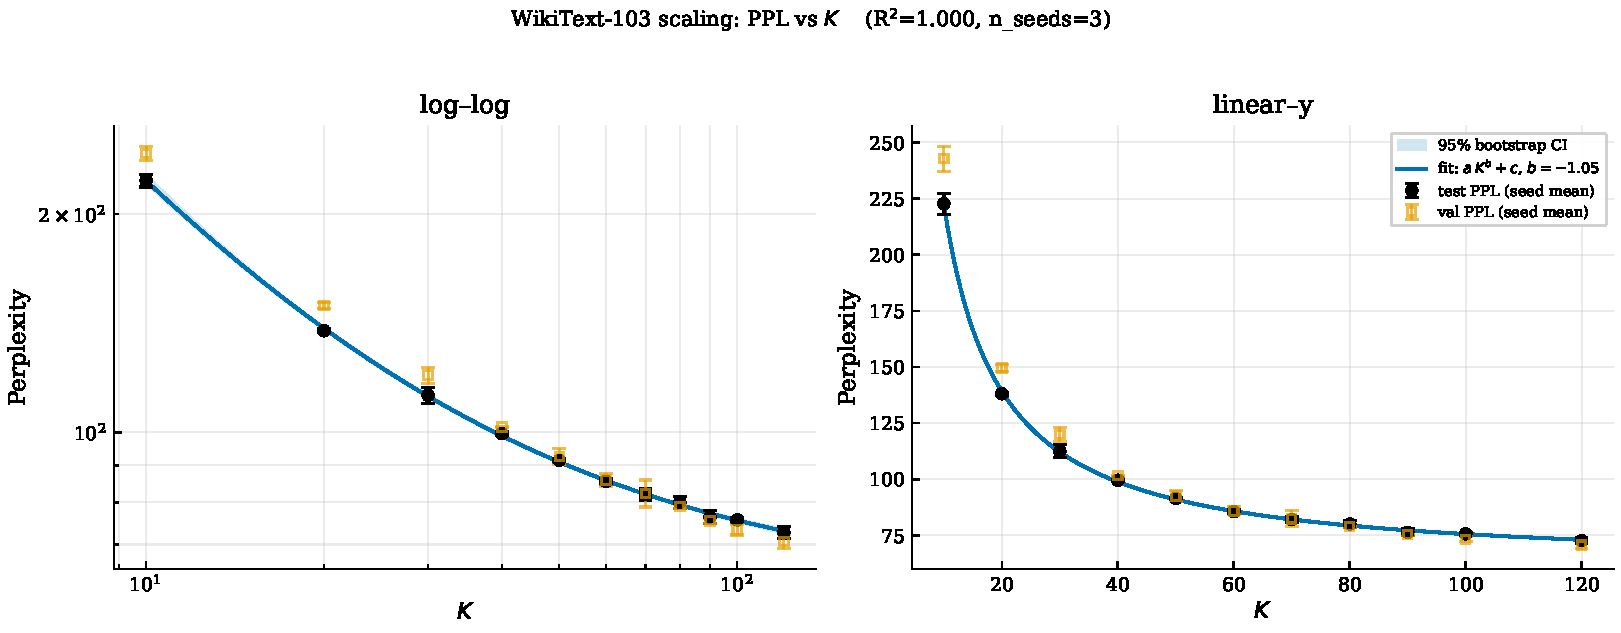
\includegraphics[width=0.75\linewidth]{fig_scaling_main.pdf}
\caption{\textbf{Multi-seed scaling law on WikiText-103.} Test perplexity versus embedding dimension $K$ for three seeds (coloured points), with per-$K$ mean and 95\% bootstrap confidence band, and fitted power law $\mathrm{PPL} = 1805.55K^{-1.049} + 61.17$ (curve). Bootstrap exponent CI $[-1.103, -0.998]$; $R^2 = 1.000$ on per-$K$ seed means; iso-token budget $122.9$M tokens, $1.2$ epochs. Reproduced from \texttt{publication\_outputs/scaling\_analysis/}.}
\label{fig:scaling_main}
\end{figure}

The fitted floor $c = 61.17$ is not an architectural ceiling for this model class: the same single-layer gauge-theoretic transformer trained on the larger Japanese Wikipedia corpus (about one billion tokens, roughly an order of magnitude more data than the iso-token budget used here) reaches test perplexities in the $15$ to $30$ range across comparable embedding dimensions, indicating that the WikiText-103 floor reflects an undertrained-convergence regime at $1.2$ epochs rather than a structural limit of the architecture. Direct cross-dataset comparison is qualified by tokeniser and language differences (gpt2 BPE 50,257-vocabulary versus cl100k\_base 100,277-vocabulary; English versus Japanese), but the order-of-magnitude data gap is large enough that data quantity dominates the comparison, leaving the $b \approx -1$ exponent as the primary architectural fingerprint that survives across regimes. The $b = -1.049$ exponent corresponds to losing roughly $2.4$ nats per decade of $K$; for context, Chinchilla-style cross-entropy scaling against total parameter count $N$ has exponent $\approx -0.34$~\cite{HoffmannChinchilla2022} corresponding to roughly $0.7$ nats per decade of $N$ at typical excess-loss values. The two exponents are not directly comparable because $K$ is embedding dimension rather than total parameter count and the gauge model has no learned attention projections (no $W_Q, W_K, W_V$); the $K$-to-$N$ map is therefore approximately linear here while in a standard transformer it is approximately quadratic.

\subsection{Training Dynamics and Convergence}

Figures~\ref{fig:train_baseline}, \ref{fig:train_gauge}, and \ref{fig:train_vfe} show training and validation loss evolution over 100 training steps for all three architectures. The standard transformer baseline (Figure~\ref{fig:train_baseline}) exhibits smooth convergence with Adam optimizer, reaching a validation loss plateau of approximately 3.12 around step 20. The gauge attention architecture (Figure~\ref{fig:train_gauge}) demonstrates nearly identical dynamics, confirming that replacing dot-product attention with KL divergence-based coupling does not impair learning when combined with standard backpropagation. Most significantly, the full gauge VFE architecture (Figure~\ref{fig:train_vfe}) achieves comparable convergence despite using only geometric updates through natural gradient descent on statistical manifolds, reaching similar validation loss by step 20 and ultimately achieving the lowest final loss of approximately 2.83 by step 100.

All three architectures show stable training at the 100-step horizon shown, with training and validation curves tracking closely throughout optimization; we make no claim about absence of overfitting at longer training horizons that we have not explored. The comparable convergence rates despite qualitatively different optimization mechanisms - standard backpropagation with Adam versus natural gradient flow on the Fisher-Rao metric - suggests that information-geometric principles may underlie the effectiveness of both approaches.The competitive performance of the full gauge VFE at this small scale provides preliminary, proof-of-principle evidence for our theoretical claims.

\begin{figure}[t]
    \centering
    \includegraphics[width=0.65\linewidth]{Fig_9.png}
    \caption{Training and validation loss evolution for standard transformer baseline with Adam optimizer. The architecture converges smoothly to validation loss $\approx 3.12$ by step 20, exhibiting typical neural network training dynamics. Close tracking between training and validation curves indicates proper generalization without overfitting.}
    \label{fig:train_baseline}
\end{figure}

\begin{figure}[t]
    \centering
    \includegraphics[width=0.65\linewidth]{Fig_10.png}
    \caption{Training and validation loss evolution for gauge attention architecture with KL-divergence weights and standard feed-forward layers. Convergence dynamics are nearly identical to the standard baseline (Figure~\ref{fig:train_baseline}), achieving validation loss $\approx 2.99$. This demonstrates that information-theoretic coupling via KL divergence can directly replace dot-product attention without impairing learning when combined with backpropagation.}
    \label{fig:train_gauge}
\end{figure}

\begin{figure}[t]
    \centering
    \includegraphics[width=0.65\linewidth]{Fig_11.png}
    \caption{Training and validation loss evolution for full gauge VFE with natural gradient descent on statistical manifolds. Despite using only geometric updates without learned weight matrices, the architecture achieves comparable convergence by step 20 and lowest final loss ($\approx 2.83$) by step 100. This validates that variational free energy minimization on gauge-theoretic statistical manifolds can match or exceed standard neural network performance, at least at small scales.}
    \label{fig:train_vfe}
\end{figure}

\section{Discussion}
\label{sec:implications}

Our framework unifies Wheeler's participatory universe, Friston's Free Energy Principle, gauge theory, and transformer architectures into a single mathematical structure. We now explore the far-reaching implications for physics, machine learning, linguistics, consciousness, and the nature of scientific knowledge itself.

\subsection{Why Was the Kinetic Term Missed?}

The kinetic term $\frac{1}{2}d\mu^T \Sigma^{-1} d\mu$ is second-order in the belief update. Standard treatments of active inference and variational free energy minimization employ first-order gradient descent, implicitly taking the overdamped limit in which inertial terms are negligible. In the mechanical analogy, this corresponds to

\begin{equation}
m\ddot{q} + \gamma\dot{q} = -\nabla V \quad \xrightarrow{m/\gamma \to 0} \quad \gamma\dot{q} = -\nabla V,
\end{equation}

where the mass-to-damping ratio vanishes and acceleration becomes instantaneously yoked to the force. Furthermore, the framework allows agent priors to evolve dynamically.  In traditional approaches predictive models are considered fixed.

Neural systems may well operate in this regime, where synaptic time constants dominate over any inertial effects. But in our theory fundamental physics requires the full second-order structure. The oversight is natural: when modeling brain dynamics, one reasonably neglects terms that are small on biological timescales. The present work recovers these terms by treating the variational principle as fundamental rather than approximate, revealing structure that was always present but previously discarded.

\subsection{Inertial Mass and Gravitational Effects in Pullback Geometry}

We have shown that within the framework the Fisher-Rao precision plays the role of effective mass:
$M_{\text{eff}} = \kappa \cdot \mathrm{tr}(\Sigma_p^{-1})$. The same precision tensor also determines the agent's pullback metric on the base manifold, which defines the geometry the agent experiences.

In our framework, agents have no direct access to the base manifold $\mathcal{C}$ itself, it remains noumenal in the Kantian sense. What agents experience is the pullback metric

\begin{equation}
g_{\mu\nu}^{(i)}(x) = \text{pullback of Fisher-Rao metric via agent } i\text{'s section}.
\end{equation}

If gravitational effects emerge, they would manifest as curvature in this pullback geometry. Since the pullback metric is determined by $\Sigma_p^{-1}$, the same quantity that provides the effective mass would also source the curvature that the agent experiences as gravitational effects

\begin{equation}
R_{\mu\nu\rho\sigma}^{(i)}[g^{(i)}] \propto \text{functions of } \Sigma_{p,i}^{-1}.
\end{equation}

Under this identification, the equivalence principle would, if it could be derived, be consistent with the framework: inertial and gravitational mass would share a single origin in prior precision because both would be properties of the agent's experienced geometry, not of some external "true" spacetime. The conditional mood is deliberate. The argument requires (i) that gravitational effects emerge from pullback curvature (not yet shown), (ii) that this curvature couples to $\Sigma_p^{-1}$ rather than to some other functional of the section (an assumption, not a derivation), and (iii) that the scalar mass $m_{\text{eff},i} = \mathrm{tr}([M_{\mu\mu}]_{ii})/K$ used in Newtonian analogies coincides with the gravitational coupling in the same way (also assumed). The equivalence principle is therefore a possible consequence of the framework, not an automatic one.

Before consensus, different agents with different priors $\Sigma_{p,i} \neq \Sigma_{p,j}$ would experience different pullback geometries $g^{(i)}_{\mu\nu} \neq g^{(j)}_{\mu\nu}$ and thus different gravitational fields. Consensus formation via the $\gamma_{ij}$ coupling drives generative-model alignment $\mathrm{KL}(s_i\|\tilde\Omega_{ij}s_j) \to 0$, which then forces the priors $p_i$ to align as cross-scale shadows of a common meta-agent belief, causing the pullback metrics to converge: $g^{(i)}_{\mu\nu} \to g^{(j)}_{\mu\nu}$. Objective spacetime geometry emerges as the shared pullback metric at equilibrium.

Demonstrating this rigorously requires computing the induced curvature tensors in the pullback metrics; work that remains to be done. The mathematical structure is consistent with this pathway whereby the agents' experienced geometry is determined by their statistical structures, and $\Sigma_p^{-1}$ sets a characteristic scale. We do not claim the equivalence principle follows as a consequence of the present framework; we claim that no obvious obstruction within the framework prevents its derivation, and that the dependence of both inertial and metric structure on the same prior precision provides a candidate route worth investigating.

The biggest challenge is reproducing the Lorentz signature $(-,+,+,+)$ since the Fisher-Rao pullback under the $\mathrm{SO}(3)$ restriction is positive-definite. The compact-group constraint is one source of this restriction, and lifting it to $\mathrm{GL}(K)$ or $\mathrm{GL}(K, \mathbb{C})$ is a necessary first step: $\mathrm{GL}(K, \mathbb{C})$ contains the Lorentz group $\mathrm{SO}(1,3)$ as a subgroup, so a Lorentz-preserving structure is at least available. It is not by itself sufficient: the linearised 2D worked example of Section~\ref{sec:worked_signature} obtains an indefinite bilinear form only after additionally imposing an imaginary frame component along a designated temporal direction and discarding the resulting complex off-diagonal terms by a real-part projection. The construction complexifies the gauge frame, not the probability distributions; the belief fiber stays positive semi-definite throughout. We register this as an existence toy model rather than as a derivation that the framework selects Lorentzian signature.

Objectivity therefore is an emergent aspect of inter-subjective consensus. What we call "universal physical laws," "shared spacetime," and "objective mass" are the gauge-invariant structures that persist at equilibrium when agents minimize their collective free energy.  Incidentally, this mechanism (if true) offers a straightforward explanation of gauge invariance in physics: we must have gauge invariance in order to agree on our observations.

This framework naturally accounts for why human observers largely agree
on physical reality. We have converged on shared generative models $s_i$ via the inter-agent slow-channel coupling $\gamma_{ij}\mathrm{KL}(s_i\|\tilde\Omega_{ij}s_j)$, with priors $p_i$ inheriting consensus structure as cross-scale shadows of the resulting meta-agent's belief. It also explains perceptual variations: altered states (psychedelics, sensory deprivation, meditation, neurological conditions) temporarily shift an individual's generative models $s_i$ away from consensus, with priors $p_i$ following derivatively, leading to experiences of modified spacetime structure, altered causal relations, or anomalous physics. These are not pathological "hallucinations" in the sense of perceiving non-existent entities, but rather genuine differences in the pullback geometry experienced by an agent operating with non-consensus models.

The theory thus dissolves the hard boundary between "veridical perception" and "altered states". Both are valid geometries on the statistical manifold, differing only in their degree of alignment with the consensus equilibrium.

Our theories of physics are predictable because, as humans, we share predictive models of reality, and what is ultimately responsible for that sharing is the dynamical law of information geometry; the same applies to all meta-agents. The institution of science, for example, is a meta-agent of the collective constituent humans. Under dynamical renormalization this meta-agent has integrated beliefs and generative models into representations of reality which we, as lower-scale agents, cannot perceive directly. Analogously, a single brain cell does not access the human agent's perspective, predictive models, or belief fluctuations; those are higher-level meta-cognitive structures.

\subsection{Macroscopic Objects as Consensus Enforcers}

The following is an interpretive extension of the formalism beyond what the simulations of Section~\ref{sec:meta_agent_emergence} demonstrate. Macroscopic objects are not modelled directly as agents in those simulations; their description here as "agents with sharp prior covariance" is a stipulation extending the multi-scale meta-agent construction (Appendix~\ref{app:examples}) by analogy. Treat the following as a framework-internal interpretation rather than a derivation.

If our perceptions and models of reality are tentative and contingent why then does everyday physics appear objective? Our answer is that macroscopic objects enforce consensus through precision dominance.

A rock maintains extraordinarily precise self-localization with prior
covariance $\Sigma_{\mathrm{rock}} \approx \epsilon I$ where $\epsilon \sim \ell_P^2$ approaches the Planck scale. When agent $i$ interacts with the rock, the coupling term

\begin{equation}
\beta_{i,\mathrm{rock}}  \mathrm{KL}(q_i \| \Omega_{i,\mathrm{rock}}[q_{\mathrm{rock}}])
\end{equation}

contains the rock's prior precision $\Sigma_{\mathrm{rock}}^{-1}$ as the sandwich operator inside the KL, so the alignment penalty scales with this very large precision and dominates $i$'s total free energy. Agent $i$'s beliefs are forced into alignment; there is no freedom to maintain alternative priors when coupled to such a high-precision neighbour.

The apparent objectivity of macroscopic physics thus arises not from
pre-existing external reality but from epistemic anchoring: high-precision systems constrain all observers into consensus. Rocks
appear "certainly there" because their extreme self-precision leaves
No room for disagreement.

\subsection{Quantum Systems: Pre-Consensus Dynamics}

The framework as constructed operates with classical probability distributions (Section~\ref{sec:scope_limitations}). The following sketch reads quantum measurement as pre-consensus dynamics in the agent picture, but the actual derivation of wavefunction collapse from classical Bayesian agents requires extending the framework to include quantum superposition states, which we have not done. Treat the following as a motivational reading awaiting a quantum extension rather than a derivation of measurement.

Quantum systems, in this reading, represent the opposite regime from the macroscopic-object case where agents have not yet established consensus. Consider a particle before measurement, with different observers maintaining different priors:

\begin{itemize}
\item Observer $A$ expects localization near $x_0$:
      $p_A(x) = \mathcal{N}(x_0, \sigma_A^2)$
\item Observer $B$ expects localization near $x_1 \neq x_0$:
      $p_B(x) = \mathcal{N}(x_1, \sigma_B^2)$
\item Observer $C$ has diffuse uncertainty:
      $p_C(x) = \mathcal{N}(x_{\text{avg}}, \sigma_C^2)$ with $\sigma_C \gg \sigma_A, \sigma_B$
\end{itemize}

Each observer assigns a different scalar effective mass via $m_{\text{eff}} = \mathrm{tr}(\Sigma_{p,i}^{-1})/K$ (proportional to the trace of their prior precision in the isolated-agent limit).
The particle has no observer-independent mass prior to consensus formation.

Measurement is the dynamical process by which an apparatus (itself a
high-precision macroscopic system) couples to the particle and dominates the free energy landscape, forcing all observers into agreement. What physics calls "wavefunction collapse" emerges as the transition from pre-consensus (perspectival, observer-dependent) to post-consensus (shared, objective) physics.

Our framework suggests a potential resolution to the measurement problem. What appears as discontinuous "collapse" may emerge from the continuous dynamics of precision-weighted consensus formation when a high-precision macroscopic apparatus couples to a low-precision quantum system. Demonstrating this rigorously requires extending the framework to include quantum superposition states, which remains future work.

\subsection{Relation to Existing Participatory Approaches}

Taking Wheeler's participatory universe \cite{Wheeler1990} seriously,  this perspectival structure extends several philosophical and physical
traditions.

\paragraph{Kantian Idealism.} Kant argued that space and time are not
"things in themselves" but forms of "sensuous intuition" through which the mind organizes experience \cite{Kant1781}. Our framework makes this precise: spacetime geometry is the pullback of the Fisher metric, determined by agent priors rather than existing independently.

\paragraph{Relational Quantum Mechanics.} Rovelli \cite{Rovelli1996}
argues quantum states are relative to observers. We extend this further and find that not only states but masses, geometry, temporal flow, and physical laws themselves are observer-dependent until consensus forms. Prior alignment is what creates the shared physics we mistake for objective reality.

\paragraph{QBism.} Fuchs et al.\ \cite{Fuchs2014} interpret quantum
probabilities as subjective degrees of belief. Our framework shares this spirit but provides the specific dynamical mechanism and geometry, variational free energy minimization on gauge-covariant principal bundles by which intersubjective agreement emerges from initially disparate beliefs.

\subsection{Realization of Wheeler's Program}

Beyond the pullback construction itself (Section~\ref{sec:pullback}), the framework speaks to two further strands of Wheeler's program~\cite{Wheeler1990} that bear on the broader physics-and-philosophy reading developed in this Discussion. The "participatory universe" thesis, that observers constitute rather than merely record reality, recurs in the relational and QBist readings discussed above and is given dynamical content here through the alignment couplings that drive agents to a shared geometry.

The "law without law" thesis acquires a similarly concrete form. Dynamical laws are not posited; they arise as stationarity conditions of the variational functional on a principal bundle. Gauge invariance is then a consequence of consensus rather than an axiom: agents that agree on reality must be related by elements of the structure group. The remainder of this Discussion develops the concomitant implications for transformers (Section~\ref{sec:transformers}), language and cognition, and open problems in the physical interpretation.

\subsection{Implications of Gauge-VFE Transformer}

The transformer derivation reveals that standard transformers are degenerate gauge-theoretic systems where spatial structure has collapsed to a single point. Learned weight matrices (query, key, value projections) approximate gauge transformations and belief representations that our framework computes explicitly. The feed-forward network approximates variational inference - the self-consistency term $\sum_i \alpha_i \mathrm{KL}(q_i \| p_i)$ drives beliefs toward priors, implementing Bayesian inference without learned parameters.

Positional encoding in standard transformers restores sequence structure through explicit embeddings. In the full framework, positional information is intrinsic to the agents' gauge frames, eliminating the need for separate positional encoding mechanisms.

The gauge-theoretic framework provides structure beyond what standard transformers capture. Beliefs are properly understood as smooth sections of associated bundles rather than vectors in Euclidean space, with all the geometric structure this entails. Transport operators enable consistent comparison across different internal reference frames, resolving the frame-dependence that would otherwise render belief comparisons meaningless. Natural gradients provide coordinate-independent optimization that respects the intrinsic geometry of statistical manifolds. The framework naturally accommodates multi-scale emergence, allowing hierarchical structure beyond flat attention patterns. The pullback construction connects information geometry to induced metric structure on base manifolds, providing the "it from bit" mechanism discussed in Section~\ref{sec:pullback}.

Standard transformers represent the zero-dimensional, gauge-fixed, single-scale limit of this richer geometric structure. They succeed because they capture the essential information-theoretic core, but they omit the geometric content that could enable more sophisticated spatial reasoning, hierarchical abstraction, and emergent geometric structure. The framework suggests that neural architectures are computational approximations to deeper information-geometric principles. Standard transformers succeed not because of clever engineering tricks but because they approximate variational free energy minimization on statistical manifolds using the attention mechanism of agent-coordination. This reframes deep learning as the discovery of efficient algorithms for information-theoretic inference rather than the design of novel computational primitives.

Several directions for extending transformers emerge naturally. Activating gauge structure with $G \neq \{e\}$ yields gauge-theoretic transformers with explicit frame transformations between agents, potentially enabling better handling of perspective-dependent or coordinate-system-dependent representations.  Enabling hierarchical meta-agent formation may produce transformers with emergent abstraction levels determined dynamically through consensus detection rather than fixed architectural choices. Incorporating the model alignment term $\gamma_{ij} \mathrm{KL}(s_i \| \tilde{\Omega}_{ij}[s_j])$ encourages agents to align not just beliefs but underlying generative models, potentially useful for multi-agent systems or continual learning. We have considered only the 0-dimensional transformer limit here; yet our framework allows the possibility of "fields" of transformers wired together via innate gauge fields or induced connections on the base manifold.

These extensions may prove relevant for several emerging research directions. Multi-agent AI systems requiring ontological alignment could benefit from explicit model coupling. Hierarchical world models with emergent abstraction arise naturally from consensus detection. Embodied AI with spatial and geometric structure connects naturally to the gauge-theoretic formalism. Cognitive architectures with multiple timescales align with the framework's natural separation between fast beliefs, slow priors, and very slow frame adjustments. The validation of transformers as a special case provides justification that extensions of the framework may yield practical architectures rather than merely theoretical and philosophical constructions.

\subsection{Implications for Language and Cognition}

\subsubsection{Language as Multi-Agent Coordination}

The success of gauge-theoretic transformers on language modeling suggests a potentially profound interpretation: language may be at root a multi-agent coordination problem solved through information-theoretic coupling. In this view, each token functions as an autonomous agent maintaining probabilistic beliefs $q_i$ about semantic content, a linguistic generative model $s_i$ encoding grammar and semantic structure, and an internal gauge frame $\phi_i$ defining its semantic coordinate system. The token-level priors $p_i$ realised as PriorBank entries in the transformer limit are then the cross-scale shadows of the corpus-level meta-agent's belief field; the grammar-and-semantics structure that gets shared across speakers is carried by $s_i$ via the model-channel coupling $\gamma_{ij}\mathrm{KL}(s_i\|\tilde\Omega_{ij}s_j)$.

Tokens attend to each other by computing coupling weights $\beta_{ij}$ to minimize collective free energy, arriving at mutually coherent interpretations. This resembles what linguists call pragmatic communication: agents coordinate to jointly minimize uncertainty and establish shared meaning. The framework thus provides a mathematical formalization of informal ideas about language as cooperative inference.

\subsubsection{The Gauge Curvature Conjecture}
\label{sec:gauge_curvature_conjecture}

\emph{Regime~II conditional.} The conjecture below is meaningful only in the Regime~II extension of the framework (Sections~\ref{sec:connection_forms} and~\ref{sec:discrete_regime_ii}), in which the connection is promoted to an independent variable not constrained to factor as $U^{-1}dU$. In Regime~I the curvature $F_{\mu\nu}$ vanishes identically by the Maurer--Cartan identity (Theorem~\ref{thm:vanishing_holonomy}), so a curvature-minimization principle has no content under the present implementation. The conjecture is therefore a conditional prediction: \emph{if} the Regime~II edge-relaxed cocycle of Section~\ref{sec:discrete_regime_ii} is realised for natural language, \emph{then} linguistic evolution should drive the Wilson observable $W_{ijk} = \operatorname{Re}\operatorname{Tr}(H_{ijk})$ of \eqref{eq:wilson_observable} toward its maximal value $K$ (vanishing holonomy, the Regime~I limit). The discrete Wilson observable is the concrete experimental probe of the conjecture; it is well-defined for any learned connection field $\delta_{ij}$, but acquires direct dynamical content for bidirectional/encoder attention rather than purely autoregressive (causal-DAG) attention, where the holonomy is an index-space invariant of the connection tensor rather than a property of the data flow.

We propose a potentially falsifiable conjecture: in the Regime~II extension, language is a gauge theory and linguistic evolution is driven by minimization of gauge field curvature. More broadly, we conjecture that informational systems with non-trivial connection structure evolve toward flat gauge structures, as curvature represents inefficiency in information transport.

The gauge field curvature measures path-dependence of information transport. For an unconstrained connection $A_\mu^{(i)}(x)$ over the token sequence or discourse structure, the field strength tensor is $F_{\mu\nu} = \partial_\mu A_\nu - \partial_\nu A_\mu + [A_\mu, A_\nu]$. Zero curvature corresponds to integrable gauge structure: information can be consistently transported between any two agents independent of the path taken through intermediate agents. Non-zero curvature indicates that the meaning transported from agent $i$ to agent $k$ depends on whether the communication path goes through intermediate agent $j$ or through agent $\ell$ (i.e. the transport is path-dependent). Under the Regime~I parameterisation $A = U^{-1}dU$ used in the present implementation, $F_{\mu\nu}$ is identically zero and "curvature minimisation" is automatic; a non-trivial linguistic curvature signal therefore presupposes the Regime~II promotion.

In natural language, gauge curvature manifests as semantic ambiguity and context-dependence. High curvature regions correspond to words or phrases whose meaning depends strongly on discourse path. This is context sensitivity in its most literal sense. Garden path sentences represent local curvature spikes that force reinterpretation when the initial parse path proves inconsistent with later information. Linguistic conventions such as grammar, morphology, and fixed phrases reduce curvature by constraining the space of possible gauge frames, making communication more robust to path variations. Creolization may provide an example: when pidgins develop into creoles with systematic grammar, we might observe rapid curvature reduction as the language acquires consistent structure.

Syntactic structure itself might emerge from the geometry of information flow. Strong attention weights $\beta_{ij}$ indicate high information coupling between tokens; thresholding this coupling matrix $A_{ij} = \mathbb{I}[\beta_{ij} > \theta]$ may yield dependency graphs that closely match syntactic parse trees. This would then suggest that syntax is not imposed by explicit rules but emerges as the skeleton of efficient information transport.  Grammar would then be an information-theoretic necessity rather than cultural convention - it is what "glues" agents into higher order meta-agents (cultures, villages, etc). This connection between information flow geometry and syntactic structure should provide ample concrete testable predictions about parsing patterns.

Beyond language, we conjecture that any system of interacting information-processing agents evolves to minimize gauge curvature as a pre-requisite for meta-agent emergence. Social systems develop shared norms and conventions that reduce curvature in social information transport. Scientific communities establish terminology, results, and notation that flatten communication gauge structure, enabling efficient knowledge transfer (beautiful examples in physics are Einstein's summation and Dirac's bra-ket notation). Neural systems meanwhile, may wire themselves to minimize curvature in neural information flow, potentially explaining observed patterns of cortical connectivity. Additionally, market economies develop institutions and contracts that reduce transaction curvature, making economic information flow more path-independent.  This principle might apply to any emergent informational system or it may only be a pretty way to describe something more ephemeral.

This gauge curvature minimization principle represents the strongest testable prediction of our framework. Unlike claims about emergent spacetime or consciousness, curvature in linguistic or social systems is measurable. One can compute field strength tensors from observed communication patterns, track curvature changes during language evolution using historical corpora, measure curvature differences between creoles and pidgins, or quantify curvature reduction in developing scientific terminology. These are concrete, falsifiable predictions that do not require solving the Lorentzian signature problem or establishing dimensional analysis. If gauge curvature fails to correlate with measures of linguistic efficiency, communicative success, or evolutionary fitness, the framework's core claim about information geometry governing real systems would be falsified.

The structural parallel is suggestive without being a unification: general relativity describes gravity as spacetime curvature, Yang-Mills theory describes fundamental forces through gauge-field curvature, and the construction here describes information systems through gauge-frame curvature on a base manifold of belief positions. Curvature drives agent alignment, alignment seeds meta-agent emergence, and the resulting hierarchy generates new curvature between meta-agents that in turn drives further alignment. Physical systems extremise action; informational systems minimise free energy, which the framework relates to gauge curvature through the variational construction of Section~\ref{sec:framework}. The shared formal structure is real and the analogy is useful, but the framework is not a unification of physical forces with cognition or language; it is a single mathematical scaffolding that admits applications in several domains.

\subsection{Gauge Invariance as Cognitive Consensus Requirement}

\paragraph{Status: this section advances a metaphysical interpretation, not a derivation.} The thesis below, that the gauge structure observed in physics is a property of human cognitive architecture rather than of the noumenal substrate, may be unfalsifiable: any observed physics can be reinterpreted as reflecting cognitive constraints, and any disappearance of gauge structure can be reinterpreted as evolutionary change in cognitive architecture rather than as evidence against the thesis. We acknowledge this at the outset rather than at the end of the section. Read the following as a permitted framework-internal interpretation that the formalism is consistent with, not as a claim the formalism establishes.

\subsubsection{The Mystery of Gauge Structure in Physics}

Modern fundamental physics is formulated as gauge theories. Electromagnetism emerges from $\mathrm{U}(1)$ gauge symmetry, the weak nuclear force from $\mathrm{SU}(2)$, the strong force from $\mathrm{SU}(3)$ quantum chromodynamics, and general relativity can be understood as a gauge theory of diffeomorphisms. This gauge structure is extraordinarily successful empirically and mathematically elegant. Yet a foundational question remains: why does nature exhibit gauge structure?

The standard answer treats gauge symmetry as a fundamental feature of physical reality: the universe simply is gauge-symmetric, and our theories reflect this objective fact. Our framework permits a different reading that inverts the traditional ontology. Gauge invariance may, in this reading, be imposed not by nature but by human cognitive architecture and the requirements of intersubjective consensus. We would discover gauge theories not because the noumenal substrate possesses gauge structure but because gauge-covariant theories are the ones that achieve stable agreement across human observers with diverse internal reference frames. As noted above, this is an interpretation the formalism is compatible with, not a claim the formalism establishes.

\subsubsection{Model Alignment and Gauge Covariance}

Recall the model alignment term in the free energy functional

\begin{equation}
\mathcal{F}_{\text{model}} = \sum_{ij} \int_{\mathcal{C}} \gamma_{ij}(x)  \mathrm{KL}\big(s_i(x) \| \tilde{\Omega}_{ij}[s_j](x)\big)  dx.
\end{equation}

This term drives alignment of generative models $s_i$ across agents. When humans construct scientific theories, they are collectively building shared models $s_{\text{human}}(x)$ that multiple agents (such as different scientists with different backgrounds, conceptual frameworks, and measurement conventions) must agree upon. The success of science depends on achieving this consensus: theories must make predictions that all qualified observers agree upon, regardless of their individual perspectives.

For model alignment to succeed, we require:
\begin{equation}
\mathrm{KL}\big(s_i \| \tilde{\Omega}_{ij}[s_j]\big) \to 0.
\end{equation}

This demands that models transform covariantly under the transport operators $\tilde{\Omega}_{ij}$ that connect different gauge frames (the model-fiber analogue of~\eqref{eq:transport_def}). In other words, scientific models must be gauge-covariant to achieve human consensus. A theory formulated in a way that depends essentially on one researcher's arbitrary internal coordinates cannot be reliably communicated to and verified by other researchers with different internal coordinates.

A gauge-invariant theory expressed in the form $\mathcal{L}[A_\mu, \psi]$ possesses the property that $\mathcal{L}[A_\mu, \psi] = \mathcal{L}[A_\mu + \partial_\mu\chi, e^{i\chi}\psi]$ under local gauge transformations. Such a theory can be transformed into any agent's reference frame and remain formally identical. This is why gauge theories prove so successful - they are cognitively shareable across humans with different internal frames. The theory's content is preserved under the transport operations necessary for inter-agent communication.

Conversely, a theory that depends explicitly on gauge choices - suppose $\mathcal{L}[\phi_i, A_\mu] \neq \mathcal{L}[\phi_j, A_\mu + \partial_\mu\chi]$ - cannot achieve consensus. Different scientists would derive different predictions from the "same" theory because the theory content fails to transport consistently across their internal reference frames. Such theories would fail empirical validation not necessarily because they incorrectly describe the noumenal substrate but because they are not cognitively compatible with human distributed information processing. They represent forms of knowledge that human cognitive architecture cannot stably share.

\subsubsection{Gauge Invariance as Selection Criterion}

Throughout the history of physics, successful theories have been selected based on several criteria. Empirical accuracy - matching observations - is the most obvious requirement. Mathematical consistency and internal coherence constitute another essential criterion. But there exists a third, rarely made explicit: inter-subjective share-ability across observers with diverse perspectives.

Newtonian mechanics achieved consensus by formulating laws Galilean-covariant under the inertial-frame transformations relating different observers. Maxwell's electromagnetism succeeded partly because its equations maintain form under Lorentz transformations, enabling observers in different reference frames to agree on electromagnetic phenomena. Einstein's relativity made coordinate independence a foundational principle, explicitly requiring that physical laws take the same form in all reference frames. Quantum field theory elevated gauge invariance to the defining structural principle.

We propose that this progression reveals not just mathematical elegance but cognitive necessity. Gauge invariance appears repeatedly in successful physics because only gauge-invariant theories can achieve stable consensus among human physicists operating with different internal reference frames. The selection pressure for gauge structure comes not from nature but from the requirements of human collaborative knowledge construction.

This suggests a revolutionary reinterpretation that gauge invariance is not a property of the noumenal substrate $\mathcal{C}$ but an emergent property of human collective cognition. We discover gauge theories because our generative models $s_{\text{human}}$ must align across individuals, and this alignment enforces gauge covariance. The noumenal reality may possess no intrinsic gauge structure whatsoever. Gauge structure appears in our scientific theories because it constitutes the mathematical form that our distributed cognitive architecture can construct and maintain consistently.

\subsubsection{Altered States and Non-Gauge-Invariant Perception}

This cognitive interpretation finds striking support from altered states of consciousness. Psychedelic experiences induced by substances like psilocybin, LSD, or DMT as well as trauma (stroke, etc) frequently involve perceptions that violate standard physical laws~\cite{Carhart-Harris2014,Swanson2018}. Users report observations seemingly incompatible with gauge-invariant or Lorentz-invariant physics such as objects merging and separating, causality flowing backwards, spatial distances becoming meaningless, temporal ordering dissolving.

The conventional view treats these as pathological - mere hallucinations reflecting disrupted brain function with no epistemic value. Our framework suggests a different interpretation. Psychedelic states may represent temporary shifts in cognitive gauge frames $\phi_{\text{human}}$ that break alignment with consensus reality. The altered perceptions are not necessarily "false" in an absolute sense but rather reflect belief states $q_{\text{altered}}(x)$ that fail to satisfy gauge covariance with the collective human prior $p_{\text{consensus}}(x)$.

Under psychedelics, an individual's gauge frame $\phi_{\text{altered}}$ may diverge significantly from the standard human gauge frame $\phi_{\text{normal}}$. The transport operator $\tilde{\Omega}_{\text{altered,normal}}$ connecting these frames develops large gauge field strength, making consistent communication nearly impossible. The psychedelic observer pulls back a radically different induced metric $G_{\text{altered}}$ that need not respect Lorentz invariance, conservation laws, or other symmetries we associate with physical law. From their phenomenal perspective, the non-gauge-invariant observations are entirely real and valid.

These experiences are "pathological" only relative to consensus reality as they represent breakdowns of the alignment that normally enables shared physical worldview. However, they reveal that human perception is capable of generating alternative phenomenologies with different geometric and causal structures. The fact that such states are unstable and non-reproducible across observers explains why they don't generate stable scientific knowledge, not that they access "false" information about an objective reality.  This raises the following thought experiment:

\subsubsection{Evolutionary Thought Experiment: Alternative Consensus Realities}

Suppose human cognitive architecture underwent evolutionary change, perhaps through genetic drift, environmental pressure, or cultural evolution. The collective human gauge frame $\phi_{\text{human}}$ shifts gradually from its current configuration to some $\phi_{\text{future}}$. If this shift occurs coherently across the population (perhaps through shared developmental environments or neural plasticity adaptations), humans might collectively pull back a different induced metric $G_{\text{future}}$ from their beliefs.

What we currently perceive as gauge-invariant, Lorentz-invariant physics might give way to alternative phenomenologies with different symmetries, different causal structures, different conservation laws. The "laws of physics" would change not because the noumenal substrate $\mathcal{C}$ changed but because human information processing architecture changed, inducing different geometric and causal structure through the pullback mechanism.

This scenario connects to predictive-processing views of perception in cognitive neuroscience, of which there are two distinct strands. The weaker "controlled hallucination" reading~\cite{Clark2016,Seth2021} holds that perception is active construction of useful models that nevertheless approximately track external structure. The stronger Interface-Theory reading~\cite{Hoffman2019} holds that evolved perception is selected for fitness rather than veridicality and need bear no faithful relation to a noumenal substrate. Different neural architectures would, under either reading, construct different perceptual models that remain internally consistent and empirically adequate relative to their own sensory evidence; the framework here makes this geometrically explicit through agent-dependent pullback metrics.

If humanity evolved toward alternative neural architectures with different inferential biases, our collective physics would shift accordingly. We would still build gauge theories, but the gauge groups might differ. We might still discover conservation laws, but conserve different quantities. We would still seek mathematical elegance and empirical adequacy, but judge these criteria differently. The physics we construct reflects not just external constraints but the structure of our information-processing architecture.

\subsubsection{Physics as Theory of Informational Compatibility}

This reframing suggests that physics is a theory of language and informational compatibility rather than a description of external substance. Physical laws are grammatical rules for constructing shareable descriptions within the constraints of human cognitive architecture. Gauge invariance, Lorentz invariance, conservation laws, and other structural features emerge as necessary conditions for maintaining consensus across diverse observers, not as intrinsic properties of a mind-independent reality.

This does not render physics arbitrary or relativistic in the negative sense. Consensual physics remains highly constrained - not all possible theories achieve stable consensus, and empirical observation strongly constrains which theories succeed. The constraints arise from both sensory evidence (observations $o$ must be compatible with the theory) and cognitive architecture (theories must satisfy gauge covariance for inter-agent alignment). Physics is objective in the sense that it achieves robust consensus, but this objectivity is social-cognitive rather than metaphysically realist.

Different intelligent species with radically different cognitive architectures might construct incompatible physics from the same noumenal substrate. They would not be wrong while we are right, or vice versa. Both physics would be valid phenomenologies (i.e.internally consistent, empirically adequate, and conducive to technological application) but incommensurable due to qualitatively different gauge structures reflecting different cognitive architectures.

\subsubsection{Implications and Limitations}

This cognitive explanation for gauge structure has several implications. It explains why gauge theories are ubiquitous in fundamental physics despite gauge structure seeming mathematically baroque - gauge covariance is the form that cognitive consensus takes. It explains why physical constants appear universal across all human measurements as they reflect shared cognitive architecture, not properties of nature independent of observers. It suggests that alternative forms of physics might be possible with different symmetries and conservation laws, though unstable within human cognitive ecology.

However, limitations must be acknowledged. While $\mathrm{GL}(K)$ is the natural gauge symmetry of KL-based variational inference, and while $\mathrm{GL}(K, \mathbb{C})$ contains the Standard Model gauge groups $\mathrm{U}(1) \times \mathrm{SU}(2) \times \mathrm{SU}(3)$ as subgroups, the framework does not yet predict \emph{which specific} subgroups are dynamically selected. It does not explain fine-tuning of physical constants or why certain symmetries are exact while others are approximate. It provides no mechanism for testing the counterfactual: we cannot experimentally alter human cognitive architecture to verify that physics would change accordingly.

Above all, this view may be unfalsifiable. Any observed physics can be interpreted as reflecting cognitive constraints rather than external reality. If gauge structure disappeared from observations tomorrow, we could claim human cognitive architecture evolved, not that our theory was wrong. This interpretive flexibility suggests the framework functions as philosophical perspective rather than scientific hypothesis in the Popperian sense.

Nevertheless, the cognitive interpretation offers novel perspectives on perennial questions. Why do we find elegant symmetries? Because symmetry represents maximal informational shareability. Why does physics seem "unreasonably effective"? Because effective physics is physics that achieves stable consensus among human observers representing a selection criterion built into the framework from the start.

Whether this constitutes genuine explanation or merely relabeling remains debatable. But it provides a coherent alternative to metaphysical realism that takes seriously both information-theoretic foundations and the observer-dependence of physical law. In Wheeler's "participatory universe," observers do not merely measure but partly constitute physical reality through their cognitive architecture and consensus-building processes. Our framework provides mathematical structure for this participation.

\subsection{Consciousness and Hierarchical Information Integration}
\label{sec:consciousness_section}

\subsubsection{Meta-Agent Structure and Conscious Experience}

Our multi-scale framework provides a formal approach to modeling aspects of consciousness, though we emphasize this remains highly speculative. In this interpretation, conscious systems correspond to meta-agents at scale $s$ that maintain explicit representations of their constituent agents at scale $s-1$. A meta-agent integrating information from multiple sensory modalities (vision, audition, proprioception) and cognitive subsystems (memory, attention, emotion) through free energy minimization exhibits the informational structure characteristic of unified conscious experience~\cite{Tononi2004,Dehaene2014}.

Self-awareness emerges naturally in this framework as recursive meta-representation. A scale-2 meta-agent observing its constituent scale-1 meta-agents, which themselves observe scale-0 base processes, exhibits the nested observational structure associated with self-reflection. The system maintains beliefs about its own beliefs producing a second-order representation enabling meta-cognition. This formal structure captures key features of self-aware systems without requiring additional mysterious ingredients beyond information integration and hierarchical organization~\cite{Cleeremans2007}.

The unity of consciousness and the fact that diverse sensory inputs and cognitive processes produce a single coherent experiential field rather than disconnected fragments, corresponds to meta-agent formation through consensus alignment. When constituent agents achieve sufficient coherence (high $C_{\text{belief}} \cdot C_{\text{model}}$), they form a unified meta-agent. Breakdown of this coherence, as in certain neurological conditions or split-brain patients, produces fragmented phenomenology~\cite{Bayne2010}.

\subsubsection{Qualia as Gauge-Frame-Dependent Phenomenology}
\label{sec:qualia}

\emph{Throughout this subsection the gauge frame $\phi_i$ is invoked in Role B (frame-as-state, Section~\ref{sec:agents_as_sections}): individual frames carry phenomenal content rather than serving as redundant labels. The induced metrics $G_i$ used below are accordingly frame-dependent (gauge-covariant) rather than gauge-invariant; the gauge-invariant correlate of phenomenal geometry, when one is needed, is the consensus / Haar-averaged metric of Section~\ref{sec:consensus_metric}.}

The framework suggests a formal and mathematical approach to qualia; the subjective, qualitative aspects of conscious experience that constitute "what it's like" to see red, taste coffee, or feel pain. Different gauge frames $\phi_i$ induce different metrics $G_i = \sigma_i^* g_{\mathcal{B}}$ through pullback from the same noumenal substrate $\mathcal{C}$. The phenomenal character of experience then corresponds to the specific geometric structure of this induced metric.

Two agents (or two sensory modalities within one agent) operating with different gauge frames perceive different phenomenal geometries despite sampling the same underlying information. The redness of red is the phenomenological signature of how visual cortex pulls back color information using its particular gauge frame $\phi_{\text{visual}}$. The painfulness of pain reflects how nociceptive processing pulls back tissue damage information using $\phi_{\text{pain}}$. These experiences feel different because the induced geometries differ, not because they access qualitatively different noumenal content.

This approach parallels inverted spectrum thought experiments in philosophy of mind~\cite{Shoemaker1982}. Two individuals might pull back inverted colour geometries from identical physical wavelength information if their visual systems employ related but distinct gauge frames. The framework formalises this possibility where qualitative inversion corresponds to gauge transformations that preserve informational structure while altering phenomenal character.

\paragraph{Qualia indeterminacy: a feature on relational readings, an open problem here.}
The group-theoretic gauge invariance built into the formalism does not, on its own, single out which gauge frame $\phi$ produces which quale. If $\phi_{\text{visual}}$ induces a metric whose geometric structure one wished to identify with "redness", gauge equivalence means that any $\phi' = \phi + \xi$ (or, equivalently, any $G' = \Omega \cdot G \cdot \Omega^\top$ for $\Omega \in \mathrm{GL}(K)$) produces the same free energy and the same empirical predictions. Read through Lahav and Neemeh's relational physicalism, this is exactly what dissolves the hard problem rather than what limits the proposal: there is no observer-independent fact about which gauge frame produces redness, and the demand for one presupposes the absolutist framing the relational reading rejects. Asking the formalism to pin down the assignment is, on that reading, a category error. The pan-agentic structuralism committed to here takes a different route. Each agent occupies a definite, multi-scale gauge-frame structure within the hierarchy of Section~\ref{sec:participatory}: a scale-$N$ meta-agent has a particular $\phi_I^{(s+1)}$ together with a definite set of constituent frames $\{\phi_i^{(s)}\}$ and consensus weights, and the cross-scale composition $\Omega_{i,I} = \exp(\phi_i^{(s)}) \exp(-\phi_I^{(s+1)})$ is fixed once the constituents are. The qualia assignment is then conjectured to be fixed by this concrete cross-scale constituent structure rather than by any group-theoretic invariant computed at a single scale; whether the variational dynamics actually pin the assignment in this way is an open research question, and we flag it as the principal piece of explanatory work the structuralist commitment still owes. The two readings are not in opposition: the relational route declares the indeterminacy constitutive, the structuralist route accepts it at the level of the symmetry group and locates the assignment one level down, in the agent's specific multi-scale composition. The honest divergences from Lahav and Neemeh are catalogued in Section~\ref{sec:lahav_convergence}.

\subsubsection{The Hard Problem Reconsidered}

Chalmers' hard problem of consciousness~\cite{Chalmers1995,Chalmers1996} asks why physical information processing should be accompanied by subjective experience at all. Why doesn't all this neural computation occur "in the dark," without any felt quality? This explanatory gap between objective physical process and subjective phenomenal experience has motivated dualist and mysterian positions claiming consciousness resists scientific explanation.

Our framework offers a \emph{relocation} of the hard problem rather than a solution. We are deliberate about that word. If one begins with physics as fundamental and tries to derive experience from it, an explanatory gap appears: no amount of physical description seems to capture subjective quality. In the present framework, physics is not the starting point; it is itself an observer-dependent pullback from the information geometry on the underlying bundle. Experience is identified, conjecturally, with the intrinsic structure of that information geometry as accessed from within a particular gauge frame. The hard problem then reappears, in a moved location: why does information-geometric structure have phenomenal character at all? The framework relocates the question from "why does neural computation feel like anything?" to "why does the geometry of inference feel like anything?".

There is, in this reading, something it is like to occupy gauge frame $\phi_i$ because that frame induces a specific metric $G_i$ defining the agent's phenomenal space. The metric is not merely formal mathematical structure but, on the conjecture this section explores, the geometric character of experience. We do not claim this resolves the explanatory gap; it shifts it.

\paragraph{Information-geometric structuralism, defined.}
The framework's ontological commitment is to \emph{information-geometric structuralism}: the substrate is the gauge-theoretic information geometry on principal bundles formalised in Section~\ref{sec:framework}, and both physical description (spacetime, fields, particles) and phenomenal description (qualia, conscious experience) are observer-dependent pullbacks from this substrate, induced by different cognitive agents acting on it through different gauge frames over the same noumenal base manifold $\mathcal{C}$. This is distinct from Russellian neutral monism~\cite{Russell1927}, which posits phenomenal intrinsic natures and treats physical structure as extrinsic; from standard physicalism, which would deny experience any privileged status in the substrate; and from panpsychism in Chalmers' later sense~\cite{Chalmers2013consciousness}, which makes phenomenal properties fundamental in their own right. Information-geometric structuralism instead grants neither physics nor experience metaphysical primacy: both are gauge-frame-dependent aspects of the same gauge-theoretic geometric structure.

The explanatory limits of this move must be stated plainly. The relocation does not explain why the information-geometric substrate has phenomenal character; it does not predict which gauge frame produces which qualitative experience (gauge invariance forbids any such pinning); and it does not constrain the inverted-spectrum or absent-qualia thought experiments any more tightly than other identity-based proposals do. The framework provides mathematical vocabulary for discussing consciousness without explaining consciousness. We flag this prominently: a reader who finds the hard problem compelling will find the relocation interesting but not satisfying.

\subsubsection{Empirical Connections and Testable Predictions}

Despite philosophical limitations, the framework suggests empirical investigations. The multi-scale structure predicts that conscious systems should exhibit robust hierarchical organization with validated top-down information flow from higher to lower scales. Neural dynamics measurements across cortical hierarchies should reveal active cross-scale coupling ($\mathcal{I}_{s \to s+1} > 0$) and prior propagation ($\Delta p_i > 0$) during conscious states. Unconscious states such as anesthesia, deep sleep, or vegetative conditions might show diminished coupling~\cite{Mashour2020,Luppi2021}.

The information integration theory of consciousness~\cite{Tononi2004,Tononi2016} provides related but distinct predictions about integrated information $\Phi$. Our framework's emphasis on hierarchical meta-agent formation and gauge-frame-dependent phenomenology offers complementary perspectives that could be empirically distinguished through appropriate experimental designs.

Conscious content richness might correlate with the effective dimensionality of induced metrics. States with richer phenomenology (vivid waking experience, certain psychedelic states) would exhibit higher-dimensional informational structure than states with impoverished phenomenology (dreamless sleep, minimally conscious states). Dimensionality reduction techniques applied to neural representations could test this prediction~\cite{Gao2017,Shine2019}.

Altered states of consciousness provide particularly interesting test cases. As previously discussed, psychedelics, meditation, sensory deprivation, and other interventions might alter gauge frames $\phi$ while leaving certain noumenal neural states relatively preserved. Changes in information-geometric properties (Fisher metric structure, transport operators, coherence patterns) during altered states could illuminate the relationship between gauge structure and phenomenal character~\cite{Carhart-Harris2014,Milliere2018}.

\subsection{Independent Convergence with Lahav and Neemeh's Relativistic Theory of Consciousness}
\label{sec:lahav_convergence}

The conclusions reached in the preceding subsection share a structural overlap with the Relativistic Theory of Consciousness developed independently by Lahav and Neemeh~\cite{LahavNeemeh2022,LahavNeemeh2025}. Their starting point is that both dualism and illusionism tacitly assume phenomenal consciousness is an absolute property, frame-independent in the way Newtonian time was once held to be. They argue that consciousness should instead be treated as relativistic: a system has phenomenal consciousness with respect to a \emph{cognitive frame of reference}, and the question whether some external system is conscious has no observer-independent answer, much as the question whether an object is at rest has no observer-independent answer in special relativity. In their Alice/Bob thought experiment, each observer measures the other as "mere brain activity" from their own cognitive frame; both measurements are correct, and the two perspectives are claimed to be related by an isomorphism between (i) Alice's first-person phenomenal state in her own cognitive frame, and (ii) Bob's third-person measurement of Alice expressed in his cognitive frame. The hard problem is taken to dissolve, on their account, once the absolutist assumption is dropped.

\paragraph{Pan-agentic extension as substantive divergence.}
The principal point of departure is best stated at the outset rather than buried in a list of caveats. Lahav and Neemeh's account is single-scale: the carriers of cognitive frames are cognitive systems in roughly the human-cognitive sense, and the relativistic move is to deny those frames any privileged status relative to one another. The framework developed here makes the stronger commitment that there are no non-agent physical things at all. Every system at every scale is an agent with its own gauge frame: scale-0 electrons, molecules, cells, brains, and ecosystems each carry a tuple of primitive fields $(q, s, \phi)$ (with priors $p$ and hyper-priors $r$ as cross-scale shadows) and a section $\sigma$ of the associated bundles, and the constituent--meta-agent transport $\Omega_{i,I} = \exp(\phi_i^{(s)}) \exp(-\phi_I^{(s+1)})$ of Section~\ref{sec:participatory} unifies cross-scale and intra-scale gauge transformations under a single group action. Lahav and Neemeh's cognitive frames of reference are then recovered as one slice of a multi-scale hierarchy (the slice at the human-cognitive scale) rather than as the ontological furniture of the theory. This is a pan-agentic structuralist commitment, not a relational physicalist one, and it does substantive work below: the Alice/Bob isomorphism is derivable as a composition of transports, and the qualia-indeterminacy worry that the relational reading dissolves is relocated rather than dissolved.

\paragraph{Recovering Alice/Bob as a derived special case.}
Within the pan-agentic framework, the structural map Lahav and Neemeh assert between Alice's first-person phenomenology and Bob's third-person measurement is recovered as a composition of two transports, neither of which is assumed: both are instances of the unified transport law $\Omega_{ab} = \exp(\phi_a) \exp(-\phi_b)$ (Section~\ref{sec:participatory}). Take Alice and Bob as scale-$N$ meta-agents, and let Alice's neurons be her scale-$(N-k)$ constituents.

Alice's first-person phenomenal state is the section $\sigma_{\mathrm{Alice}}^{(N)}$ together with the pullback metric $G_{\mathrm{Alice}} = (\sigma_{\mathrm{Alice}}^{(N)})^* g_{\mathcal{B}}$ that her scale-$N$ frame $\phi_{\mathrm{Alice}}^{(N)}$ induces on $\mathcal{C}$. Bob's third-person observation of Alice is not a measurement of $\sigma_{\mathrm{Alice}}^{(N)}$ directly but of Alice's scale-$(N-k)$ constituents, expressed in Bob's scale-$N$ frame $\phi_{\mathrm{Bob}}^{(N)}$. The map between the two readings factors as
\begin{equation}
\Omega_{\mathrm{Bob}, i}
=
\underbrace{\exp(\phi_{\mathrm{Bob}}^{(N)}) \exp(-\phi_{\mathrm{Alice}}^{(N)})}_{\text{inter-agent, scale-}N}
\cdot
\underbrace{\exp(\phi_{\mathrm{Alice}}^{(N)}) \exp(-\phi_{i}^{(N-k)})}_{\text{cross-scale, Alice-internal}},
\end{equation}
where $\phi_i^{(N-k)}$ is the frame of an Alice-neuron and the cross-scale piece is fixed by the consensus-aggregation construction of $\phi_{\mathrm{Alice}}^{(N)}$ from its constituents (Section~\ref{sec:participatory}). The cross-scale factor is what relates Alice's first-person scale-$N$ section to the scale-$(N-k)$ neural substrate Bob actually probes; the inter-agent factor is what carries the result into Bob's frame. Lahav and Neemeh's single-scale Alice/Bob isomorphism is recovered as the special case in which both observers and the observed system are taken at the same scale and the cross-scale factor reduces to the identity. The structural map their account asserts is, in the present framework, a derived composition rather than a posited isomorphism, and the formalism specifies exactly which two transports it is built from.

\paragraph{Three points of mathematical contact.}
The transformation between cognitive frames is concrete: $\Omega_{ij}$ acts on belief means by left multiplication and on covariances by the sandwich product $\Omega_{ij} \Sigma_j \Omega_{ij}^\top$, and KL divergences are invariant under simultaneous push-forward by any element of $\mathrm{GL}(K)$. The analogue of a frame-invariant quantity (the role played by the spacetime interval in special relativity) is the gauge-equivariant free energy itself: $\mathcal{F}$ is a scalar under the diagonal action of $\mathrm{GL}(K)$, even though its constituent KL terms transform between frames. The postulate that "identical neural dynamics imply identical experience" becomes, in our setting, the statement that two agents with identical $(\mu, \Sigma, \phi)$ at the relevant scale occupy the same section and therefore induce the same pullback metric; the postulate is recovered as a consequence of section identity rather than imposed.

We do not claim our gauge frames \emph{are} Lahav and Neemeh's cognitive frames in any stronger sense than that the two notions play the same conceptual role. Their cognitive frame is a measurement perspective taken as primitive; our gauge frame is a particular element of $\mathfrak{gl}(K)$ that determines a section of an associated bundle of belief tuples. The match is at the level of structural function, not ontological identity. Where we can offer mathematical content beyond what their published formalization provides  (an explicit non-compact transformation group, an explicit invariant scalar, an explicit covariance transport law, and an explicit account of why first-person and third-person measurements relate the way they do) we view this as complementary to rather than competitive with their proposal. The intellectual debt runs in the opposite direction: their reframing of phenomenal consciousness as a frame-relative quantity is the philosophical move that licenses the construction in this paper.

\paragraph{Divergence I: substance and ontology.}
Lahav and Neemeh are best read as relational physicalists: physical reality is observer-relative in its presentation but ontologically prior to and independent of any particular observation. The two sides of the Alice/Bob isomorphism are perspectives on a physical system whose reality is not itself constituted by being perspectivally accessed. The construction here commits to a stronger position, pan-agentic structuralism: there is no observer-independent physical substrate sitting underneath the agents, and physical reality is itself constituted by the gauge-theoretic information geometry of agents-at-scales (Section~\ref{sec:scope_limitations}). The substrate is the agentic structure, not a layer below it. This is in the same broad neighborhood as their relational view: both deny that physical reality is independent of cognitive frame but it is not the same view, and it should not be quoted as if it were.

\paragraph{Divergence II: pan-agentism and multi-scale extension.}
Lahav and Neemeh's relativistic move is between cognitive frames at a single scale; the question of what a cognitive frame \emph{is}, and what its carriers are, is left to the reader's intuitions about cognitive systems. The present framework takes the stronger position that there are no non-agent physical things: every electron, atom, molecule, cell, brain, and ecosystem is an agent with its own primitive $(q, s, \phi)$ and derived shadows $(p, r)$, and the Lahav-Neemeh CFRs are recovered as the human-cognitive slice of a multi-scale hierarchy whose cross-scale and intra-scale transports are unified under $\Omega_{ab} = \exp(\phi_a) \exp(-\phi_b)$ (Section~\ref{sec:participatory}). The Alice/Bob derivation in the preceding paragraph depends on this multi-scale extension: the cross-scale factor that reaches from Alice's scale-$N$ self-section down to her scale-$(N-k)$ neurons has no place in a single-scale account.

\paragraph{Divergence III: second postulate and Lorentzian signature.}
The relativistic analogy in Lahav and Neemeh proceeds without an analogue of the speed of light. Our present framework does not supply such a second postulate either. What it offers instead is a mechanism in which the frame-twist quadratic form on $\mathrm{GL}(K, \mathbb{C})$ gauge frames yields indefinite signature in a linearized two-dimensional worked example (Section~\ref{sec:signature_resolution}; the postulates of that example -- imaginary frame component on the temporal direction, non-compact generator with positive trace square, and a real-part projection on the resulting complex bilinear form -- are stated honestly, and the four-dimensional, fully nonlinear extension is left open). Whether either route reaches a fully Einsteinian rather than Galilean theory of cognitive frames remains open.

\paragraph{The qualia-indeterminacy issue, reframed.}
The qualia-indeterminacy worry that the relational reading dissolves is relocated rather than dissolved on the structuralist route adopted here: gauge invariance is constitutive at the symmetry-group level, but the specific multi-scale composition $\{\phi_i^{(s)}, \phi_I^{(s+1)}, \ldots\}$ pins the assignment one level down, in the agent's concrete cross-scale constituent structure. The full development is in Section~\ref{sec:consciousness_section}; whether the variational dynamics actually pin the assignment in the structuralist way remains an open research question.

\paragraph{The central open question.}
The pan-agentic position incurs a debt that single-scale relational accounts do not: it must say why scale-0 electrons have the same kind of belief-and-model-bearing structure $(q, s, \phi)$ as scale-$N$ humans, and why aggregating low-scale agents into high-scale meta-agents preserves rather than eliminates phenomenal properties. The consensus-aggregation mechanism of Section~\ref{sec:participatory} supplies the mathematical aggregation: it constructs $\phi_I^{(s+1)}$ and the meta-agent belief tuple from the constituent fields, and it is gauge-covariant by construction. It does not supply the phenomenal-aggregation argument: nothing in the formal construction settles whether the meta-agent's pullback metric $G_I$ inherits anything experiential from the constituent metrics $\{G_i\}$, or whether the inheritance fails at certain scale jumps, or whether scale-0 frames carry phenomenal character at all. This is the central open research question raised by the pan-agentic commitment, and it is honestly an open one: it is what would have to be done to convert the structuralist route on qualia indeterminacy from a relocation into a derivation.

\subsection{Philosophy of Science: Knowledge as Collective Free Energy Minimization}

\subsubsection{Scientific Progress Reconsidered}

Our framework suggests a reconceptualization of scientific progress and theory development. The traditional view holds that science discovers objective truths about nature through hypothesis formulation and empirical testing. Better theories correspond more accurately to external reality, with scientific progress constituting asymptotic approach to truth.

Our framework offers an alternative interpretation. Science constructs shareable generative models $s_{\text{scientific}}$ that optimize a multi-objective function. First, models must minimize KL divergence from empirical observations; this is the conventional empirical adequacy criterion. Second, models must achieve intersubjective consensus across diverse researchers, minimizing $\sum_{ij} \gamma_{ij}\mathrm{KL}(s_i \| \tilde{\Omega}_{ij}[s_j])$ through the model-alignment term. Different scientists with different backgrounds and perspectives must converge on shared models. Third, as discussed earlier, models must exhibit gauge invariance to enable cognitive shareability across different internal reference frames.

Scientific "truth" in this view is not correspondence with the unknowable noumenal manifold $\mathcal{C}$ but optimal collective free energy minimization satisfying these multiple constraints. Better theories are those that simultaneously fit observations, achieve consensus, and maintain gauge covariance. This is a pragmatic, instrumentalist reconception of scientific knowledge~\cite{vanFraassen1980,Laudan1984}.

\subsubsection{Kuhnian Revolutions as Collective Gauge Transformations}

Kuhn's analysis of scientific revolutions~\cite{Kuhn1962} describes periods of normal science punctuated by revolutionary paradigm shifts. Normal science operates within an established paradigm, solving puzzles using accepted methods and concepts. Revolutions occur when accumulated anomalies undermine the paradigm, leading to adoption of a qualitatively new framework. Kuhn controversially argued that successive paradigms are incommensurable, i.e. they cannot be directly compared or translated into each other's terms.

Our framework provides formal structure for Kuhn's informal analysis. Normal science corresponds to a period where the scientific community shares gauge frame $\phi_{\text{old}}$ with associated generative model $s_{\text{old}}$. Research proceeds through incremental refinement of this model, minimizing free energy within the established gauge structure. Anomalies accumulate when observations $o$ increasingly conflict with $s_{\text{old}}$, raising collective free energy despite ongoing efforts at accommodation.

A scientific revolution occurs as collective gauge transformation $\phi_{\text{old}} \to \phi_{\text{new}}$ with accompanying model shift $s_{\text{old}} \to s_{\text{new}}$. Early adopters develop the new framework, demonstrating that $s_{\text{new}}$ better explains observations. If successful, model-alignment pressure drives transformation through the community. Scientists adopt $\phi_{\text{new}}$ because it enables lower free energy states than maintaining $\phi_{\text{old}}$ against mounting empirical tension.

Kuhn's incommensurability thesis corresponds to large informational distance between transported beliefs across distant gauge frames. The transport operator $\Omega_{\text{old,new}}$, given by~\eqref{eq:transport_def} with frames $\phi_{\text{old}}, \phi_{\text{new}}$, remains invertible by construction (it does not "approach zero" in any operator-norm sense) but when $\phi_{\text{old}}$ and $\phi_{\text{new}}$ are sufficiently different, the KL divergence between an old-paradigm belief $q_{\text{old}}$ and its transport $\Omega_{\text{old,new}}^{-1} q_{\text{old}}$ into the new frame can be made arbitrarily large, such that meaningful translation becomes nearly impossible: concepts that minimize free energy under one frame fail to do so under the other, and the operator that formally relates them takes coherent sentences to incoherent ones. Concepts natural in one paradigm lack direct counterparts in the other. This is not mere linguistic difficulty but reflects genuine structural differences in how the frameworks organize information. Scientists on opposite sides of a revolution literally inhabit different phenomenal realities despite observing the same noumenal substrate.

This interpretation supports Kuhn's anti-realist tendencies while providing mathematical precision his informal account lacked~\cite{Hoyningen-Huene1993}. Scientific progress is real (we achieve better free energy minimization) but not necessarily truth-convergent (we may not approach objective reality, only optimized shared models).

\subsubsection{Under-determination and Theory Choice}

Quine's under-determination thesis~\cite{Quine1951,Quine1975} holds that empirical evidence alone cannot uniquely determine theory choice.  Multiple incompatible theories can fit the same observational data. This poses challenges for scientific realism, suggesting empirical adequacy is insufficient to establish theoretical truth.

Our framework formalizes and explains under-determination. Multiple gauge-invariant generative models $\{s_1, s_2, \ldots\}$ may minimize empirical KL divergence equally

\begin{equation}
\mathrm{KL}(s_1 \| o) = \mathrm{KL}(s_2 \| o) = \cdots.
\end{equation}

Since empirical fit is only one component of the free energy functional, additional criteria determine theory choice. Model alignment considerations favor theories that achieve consensus more easily across diverse research communities. Simplicity preferences select theories with lower gauge field complexity $\|\nabla\phi\|^2$.  Unification motivations seek theories operating at higher hierarchical scales, integrating previously separate domains (e.g. the fields of biology, information, and physics are separate but overlapping meta-agents composed of myriad institutions, humans, etc). Historical and sociological factors influence which theories scientists explore and how quickly communities converge.

There is no uniquely "true" theory waiting to be discovered. Rather, we construct theories optimizing collective free energy under multiple constraints. Different scientific communities (or humanity at different historical periods) might converge on different theories equally adequate empirically but divergent in other dimensions. This supports constructive empiricism~\cite{vanFraassen1980} and scientific pluralism~\cite{Longino2002} while rejecting convergent realism.

\subsubsection{Fundamental Limits of Scientific Knowledge}

The framework implies inherent epistemic limitations transcending practical or temporary constraints. The noumenal manifold $\mathcal{C}$ remains unknowable in principle. We can only access pullbacks $\sigma^* g_{\mathcal{B}}$ through our gauge frames, never the substrate directly. Kant's thing-in-itself is not just epistemically inaccessible but structureless until accessed through an agent's information-processing architecture. There exists no "view from nowhere".  Every observation, every measurement, every theoretical formulation is necessarily mediated by some gauge frame~\cite{Nagel1986}.

Physical theories exhibit gauge ambiguity.  Infinitely many gauge-equivalent formulations exist for any successful theory. These formulations are empirically indistinguishable and mathematically inter-translatable but philosophically distinct. No single formulation can be privileged as "correct" as they represent equally valid but gauge-frame-dependent expressions of the same underlying structure. This is not mere convention but reflects fundamental redundancy in how information geometry maps onto physical description.

All observations/attentions are observer-dependent in a deep sense. Different agents (or different cognitive architectures) pull back different geometries from the same substrate. Absolute objectivity is logically impossible and only inter-subjective agreement is achievable ( and only within communities sharing sufficient gauge-frame alignment).

Cognitive constraints limit which theories humanity can construct regardless of which theories might be "true" about $\mathcal{C}$. Theories must be humanly shareable (gauge-covariant) to achieve scientific consensus. Forms of knowledge requiring gauge structures incompatible with human cognitive architecture remain permanently inaccessible, not due to practical limitations but to structural incompatibility. Alien intelligences with different cognitive architectures might develop incompatible but equally valid physics from the same noumenal reality.  As a practical example, no human has ever "observed" a wave-function, yet the meta-agent of science readily accesses it and because of this humans can manipulate and access this knowledge.

These are not pragmatic limitations awaiting technological solution but fundamental epistemic constraints arising from the structure of information geometry itself~\cite{Ladyman2007}. Recognition of these limits need not promote relativism or skepticism. Within these constraints, science remains extraordinarily successful at constructing predictive, manipulable, consensus-generating models. But claims to access absolute objective truth beyond phenomenal appearances lack foundation.

\subsection{Synthesis and Future Directions}

\subsubsection{Unification Across Domains}

This gauge-theoretic active inference framework unifies diverse phenomena under a common mathematical geometry. In physics, spacetime structure and physical laws might emerge from information geometry through observer-dependent pullbacks, providing mathematical realization of Wheeler's "it from bit" vision. In machine learning, transformer attention mechanisms are revealed as degenerate gauge theories in the zero-dimensional limit, with natural gradients providing optimal learning dynamics on statistical manifolds. In linguistics and cognitive science, language might emerge as multi-agent coordination through information-theoretic coupling, with syntactic structure reflecting patterns of high information flux.

Consciousness is approached through hierarchical meta-awareness with gauge-frame-dependent phenomenology. Though this remains highly speculative it does present novel philosophical positions worth exploring. Cosmological structure in this view emerges from informational symmetry breaking and multi-scale organization. Philosophy of science reconceptualizes scientific progress as collective free energy minimization under gauge-invariance constraints, providing formal structure for Kuhnian paradigm shifts and Quinean underdetermination.

The breadth of these applications demonstrates that the framework captures genuinely general principles of information processing and organization. However, we must distinguish between rigorous derivations (transformers from gauge theory) and suggestive analogies (consciousness from meta-agents). Only transformer connections have thus far been empirically validated. Other applications remain speculative, requiring substantial development before constituting testable hypotheses.

\section{Critical Open Problems and Future Directions}
\label{sec:open_problems}

Several fundamental problems must be resolved before this framework can claim to explain physical reality rather than providing suggestive mathematical analogies.

\subsection{The Lorentzian Signature Problem}

\textbf{Problem:} Under the $\mathrm{SO}(3)$ restriction used in our simulations, Fisher-Rao geometry is intrinsically Riemannian (positive-definite), yet spacetime requires Lorentzian signature $(-,+,+,+)$.

\textbf{Existence-toy status:} As detailed in Section~\ref{sec:signature_resolution}, lifting the compact-group restriction is a necessary condition for indefinite signature on the pullback metric, but not a sufficient one. The natural gauge group $\mathrm{GL}(K)$ is non-compact yet, on real Gaussian fibers, produces positive-definite transport (Sylvester's law of inertia), so non-compactness alone does not flip the signature. The 2D worked example of Section~\ref{sec:worked_signature} obtains an indefinite bilinear form by adding three further postulates on top of the group-theoretic prerequisite: (i) one base direction is designated temporal, (ii) the corresponding gauge-frame component is multiplied by~$i$, and (iii) the imaginary off-diagonal piece of the resulting complex-valued bilinear form is discarded by a real-part projection. The construction does not extend complex values to the probability distributions $q_i$ themselves, which remain real Gaussians; only the gauge frame is complexified. The complexified gauge group $\mathrm{GL}(K, \mathbb{C})$ contains the Lorentz group $\mathrm{SO}(1,3)$ as a subgroup via $\mathrm{SL}(2, \mathbb{C}) \cong \mathrm{Spin}(1,3)$, so a Lorentz-preserving subgroup is at least available; whether free-energy minimisation selects it dynamically remains open.

\textbf{Remaining Work:} The worked example (Section~\ref{sec:worked_signature}) demonstrates the mechanism for $K=2$ on a 2D base in the linearized (weak-field) regime. Key open questions include: whether imaginary gauge frame components emerge dynamically from free energy minimization (rather than being imposed), whether the $(1,3)$ signature is naturally selected when the observable sector has four large eigenvalues, and whether the result extends beyond the linearized regime to the full non-linear Yang-Mills theory. Computational implementation of the $\mathrm{GL}(K, \mathbb{C})$ gauge transformer on a higher-dimensional base manifold would test these questions directly.

\textbf{Status:} A candidate mechanism has been identified in a 2D linearised worked example. The signature problem is not yet resolved. The construction imposes the imaginary temporal component $\phi_\tau = i\psi_\tau \cdot T$ by hand, and the diagonal-metric outcome depends on a coincidence of generator choice ($T_\tau = T_x = T$). Whether the imaginary component emerges dynamically from free energy minimisation, whether the construction generalises to four nonlinear dimensions, and whether independent generator choices preserve the Lorentzian signature, all remain open. This worked example demonstrates that an indefinite signature is at least compatible with the framework's gauge structure; it does not show that the framework derives it.

\subsection{Dimensional Structure and Physical Constants}
\label{sec:dimensional_structure}

\textbf{Philosophical Position:} In this framework, information is the dimensionally fundamental quantity. Physical dimensions (kilograms, meters, seconds) are not ontologically primitive but emerge as phenomenological labels that consensus among agents assigns to specific information-geometric structures (Section~\ref{sec:phenomenological_interpretation}). This is the "it from bit" position taken to its logical conclusion: if physical reality emerges from information dynamics, then physical units must also emerge rather than being presupposed. Demanding \emph{a priori} conversion between nats and kilograms would be circular, it would require assuming the very dimensional structure the theory claims to derive.

\textbf{The Open Problem (Reframed):} The question is not "how do we convert between nats and kilograms?" (which presupposes that both are fundamental) but rather "at what stage of the consensus hierarchy do dimensionful quantities crystallize, and what determines their specific values?" Our framework predicts that physical dimensions emerge through multi-scale consensus formation: at macroscopic scales where meta-agents achieve stable agreement on shared geometric structure, the consensus-invariant quantities acquire the operational character of physical measurements. The fundamental constants $c$, $\hbar$, and $G$ should correspond to specific information-geometric invariants of the consensus geometry such as ratios of coupling strengths, curvature scales, or information distances at characteristic hierarchical levels.

\textbf{Testable Prediction:} Dimensionless ratios between physical constants should be derivable from pure information geometry without reference to kilograms or meters, since these ratios are already unit-free. If the framework describes reality, these dimensionless numbers must emerge from the gauge-theoretic structure. The Planck length $\ell_P = \sqrt{\hbar G/c^3}$ might emerge as the minimum resolvable information distance in the induced consensus metric, providing a natural scale.

\textbf{Status:} This remains an open research program. The philosophical position (information is primal, dimensions are emergent) is internally consistent and avoids the circularity of demanding dimensional conversion within an information-first ontology. However, the framework has not yet derived any dimensionless constant from first principles. Successful derivation of even one such constant would constitute major evidence for the framework; failure to do so after sustained effort would limit its explanatory scope.

\subsection{Scaling and Phase Transitions}

\textbf{Problem:} Our largest validated system (8 agents, dimension 13) is tiny. Behavior at scale ($N>1000$, $K>768$) is unknown. Limited computational resources (a single AMD 9900x CPU) have prevented deeper explorations.

\textbf{Open Questions:} Does hierarchical emergence persist at large $N$, or does it break down beyond some critical scale? Are there phase transitions in coupling strength, consensus formation, or hierarchical structure? Do emergent phenomena appear at large scales that are absent in small systems? Can computational efficiency be improved to make large-scale simulation tractable? These questions require substantial computational resources beyond this proof-of-concept study.

\subsection{Quantum Extension}

\textbf{Problem:} The framework operates with classical probability distributions. Physical reality requires quantum amplitudes, superposition, and entanglement.

\textbf{Possible Approaches:} The $\mathrm{GL}(K, \mathbb{C})$ extension described in Section~\ref{sec:signature_resolution} provides a natural bridge to quantum structure. Complex-valued gauge frames and belief parameters introduce phases and interference effects that are absent in the real-valued formulation. The unitary subgroup $\mathrm{U}(K) \subset \mathrm{GL}(K, \mathbb{C})$ preserves Hermitian structure and is the gauge group of quantum mechanics; $\mathrm{U}(1) \subset \mathrm{U}(K)$ would naturally introduce quantum phases (the electromagnetic gauge group).  Allowing statistical manifolds with non-commutative structure could capture quantum incompatibility. Developing tensor product bundle structures might enable agent beliefs to become quantum-entangled. While structural parallels with QBism are suggestive, no rigorous quantum extension currently exists, though the $\mathrm{GL}(K, \mathbb{C})$ pathway provides concrete mathematical tools for pursuing one.

\subsection{Experimental Validation}

\textbf{Problem:} Beyond transformer validation, we lack concrete experimental proposals testing physical predictions.

\textbf{Requirements:} We need specific predictions distinguishing this framework from conventional physics, observational signatures of "induced metrics" in measurable systems, protocols for detecting or measuring "gauge frames" in cognitive or physical systems, and tests of hierarchical emergence in neural systems or collective behavior. Transformers provide one validation domain, but extensions to neuroscience, social systems, or fundamental physics require new experimental designs.

\subsection{Computational Optimization}

\textbf{Problem:} The 825× computational overhead relative to standard transformers limits practical applications.

\textbf{Possible Approaches:} Learned approximations to transport operators, structured covariance matrices reducing KL computation cost, approximate natural gradient methods, and hardware acceleration for gauge-theoretic operations might substantially improve performance. However, first-principles implementation has been achieved; engineering optimization is separate future work. We acknowledge, however, that in larger experiments the natural gradient descent may allow training convergence in far fewer steps than standard Euclidean algorithms.  For example, if gauge-attention required $1000\times$ more compute per step but converged in $1000\times$ fewer steps than a conventional approach, total cost would be comparable. Natural-gradient descent generally accelerates convergence on curved manifolds.

\section{Conclusion}
\label{sec:conclusion}

In 1990, John Archibald Wheeler asked: "How come existence?" He proposed that the answer lay in information, articulating his vision through "it from bit" and the participatory universe - the idea that observers play an active role in bringing reality into being. For over three decades, this vision remained largely philosophical, inspiring but lacking mathematical precision and empirical grounding.

We have developed a gauge-theoretic active inference framework that provides mathematical structure for exploring Wheeler's ideas. Agents are represented as smooth sections of associated bundles over two statistical manifolds, with two primitive fields (beliefs $q_i$ on $\mathcal{B}_{\mathrm{state}}$, generative models $s_i$ on $\mathcal{B}_{\mathrm{model}}$) and two derived cross-scale shadows (priors $p_i$ and hyper-priors $r_i$, obtained from the meta-agent's primitives via Eq.~\eqref{eq:cross_scale_shadow}) over a base manifold $\mathcal{C}$. These agents couple through information-theoretic interactions mediated by gauge-covariant transport operators $\Omega_{ij}$ on the state fiber and $\tilde\Omega_{ij}$ on the model fiber, minimizing collective variational free energy. The framework naturally generates hierarchical structure through consensus-driven meta-agent formation, creating bidirectional information flow between scales.

The framework's most concrete achievement is demonstrating that transformer attention mechanisms emerge rigorously as the zero-dimensional limit of gauge-theoretic variational inference. We have implemented working gauge-theoretic transformers achieving competitive performance with standard architectures on language modeling tasks, with strong empirical correlation (r=0.821) between our information-theoretic attention weights and learned BERT patterns. This validates the framework's core mathematical structure in at least one domain and establishes that practical machine learning can be understood through sophisticated gauge theory.

Beyond transformers, the framework suggests - but does not yet establish - potential connections to fundamental physics. Geometric structure on base manifolds can be induced through pullback operations from Fisher-Rao metrics, providing a toy model demonstration that spacetime-like geometry might emerge from information dynamics. Different agents with different gauge frames pull back different phenomenal geometries from the same noumenal substrate, formalizing observer-dependent reality. We have shown this is mathematically coherent and computationally implementable, though whether it describes actual physical spacetime remains entirely open.

The framework makes contact with diverse domains - linguistics as multi-agent coordination, consciousness as hierarchical information integration, scientific knowledge as collective free energy minimization, gauge invariance as cognitive consensus requirement. These applications range from rigorously developed (transformers) to suggestive analogies (consciousness, cosmology) to philosophical interpretation (epistemology, constructivism). We have attempted to clearly distinguish validated results from speculative extensions throughout.

Several limitations and open problems persist. The Lorentzian signature problem remains open. A candidate mechanism is exhibited in the worked example of Section~\ref{sec:worked_signature}: imaginary components of $\mathrm{GL}(K, \mathbb{C})$ gauge frames can produce indefinite signature on the base manifold through the frame-twist quadratic form $\mathrm{tr}(A_\mu A_\nu)$, with $\mathrm{SO}(1,1) \subset \mathrm{GL}(2, \mathbb{C})$ as the signature-preserving subgroup. The construction is 2D and linearised, the imaginary component is imposed by hand, the result depends on choosing a non-compact generator with $\mathrm{tr}(T^2) > 0$ (rather than a compact one with $\mathrm{tr}(T^2) \le 0$), and the real Lorentzian metric is recovered only after a real-part projection on the resulting complex bilinear form. Whether the mechanism arises dynamically from free energy minimisation, generalises to four nonlinear dimensions, and survives independent generator choices, all remain open. Dimensional analysis connecting information-theoretic quantities to physical units is incomplete. We make no quantitative predictions for physical constants, particle masses, or coupling strengths. Matter fields and fundamental interactions lack representation. The framework may be unfalsifiable in central domains, compatible with any observation through appropriate interpretive choices. Many claims function as philosophical interpretation rather than scientific hypothesis.

Nevertheless, the framework offers several contributions. It demonstrates that transformer architectures have deep theoretical foundations in gauge theory and variational inference, not merely empirical success. It provides mathematical precision to Wheeler's participatory universe vision, showing such ideas are not inherently mystical but can be formulated rigorously. It suggests novel perspectives on perennial problems in philosophy of science, consciousness studies, and quantum foundations. It generates concrete testable predictions in machine learning and neuroscience while offering interpretive schemas for phenomena spanning cognition to cosmology.

Whether this constitutes fundamental progress or sophisticated reformulation of existing questions remains unclear. The framework succeeds in unifying gauge theory with active inference and demonstrating practical applications. It provides new mathematical tools and conceptual vocabulary for investigating foundational questions. But whether it illuminates reality's ultimate nature or merely describes our cognitive architecture's necessary forms remains undecidable - perhaps appropriately so given the framework's own emphasis on observer-dependence and gauge-frame-relativity.

Future work must address critical gaps. Can dimensionless physical constants be derived from information-geometric first principles? Can the $\mathrm{GL}(K, \mathbb{C})$ pathway to Lorentzian signature (Section~\ref{sec:signature_resolution}) be computationally implemented and validated? Can the framework be extended to full quantum settings through complexification, with $\mathrm{U}(K) \subset \mathrm{GL}(K, \mathbb{C})$ providing quantum gauge structure? Can hierarchical meta-agent predictions be tested in neural systems? Can the computational overhead of gauge-theoretic transformers be reduced to practical levels? Each represents a concrete research program with clear success criteria. The identification of $\mathrm{GL}(K)$ as the natural gauge group has resolved one major theoretical obstacle and opened new avenues for the remaining ones.

The universe may indeed be participatory in Wheeler's sense - with observers not merely measuring but partly constituting physical structure through information-processing architecture. Our framework provides mathematical foundations for exploring this possibility with precision exceeding informal philosophical speculation. We have shown that cognitive-first ontology is mathematically coherent, computationally implementable in limited domains, and empirically testable in principle. Whether it describes how nature actually operates remains the central open question.

Wheeler opened a door in 1990 with "it from bit." We have constructed a mathematical framework and walked partway through. The path leads through gauge theory, information geometry, and variational inference toward a potential understanding of reality as emerging from informational dynamics. Whether this path reaches genuine explanation or circles back to familiar puzzles reformulated in new language, only continued investigation will reveal. But the journey itself has yielded insights - demonstrating that attention mechanisms emerge from first principles, that observer-dependent reality can be rigorously formalized, that information geometry provides powerful tools for unifying apparently disparate phenomena.

In this sense, we participate in answering Wheeler's question not by providing final solutions but by developing precise mathematical structures that transform vague ideas into testable hypotheses. The framework represents one possible formalization of participatory reality - coherent, implementable, and partially validated. Its ultimate significance will be determined not by philosophical arguments but by whether it generates novel predictions, explains previously mysterious phenomena, or enables technological applications beyond what existing frameworks provide. That assessment must await future work, but the foundations are now established for rigorous investigation of whether reality might indeed be information all the way down.

\section{Methods}
\label{sec:methods}

\subsection{Computational Details}
All simulations were implemented in Python with PyTorch automatic differentiation; gradient correctness against analytic expressions was verified by finite differences and by autograd cross-check to relative error $<10^{-8}$ (see appendix on numerical stability and verification). Hamiltonian belief dynamics for the mass-precision experiments use a velocity-Verlet symplectic integrator with energy drift $<0.001\%$ over $25$ time units. Multi-agent simulations of the Ouroboros Tower were run on a single AMD Ryzen 9 9900X CPU; large-scale gauge-transformer training (Section~\ref{sec:scaling_validation}) was run on the same machine, hence the iso-token rather than iso-FLOP budget choice. Random seeds are fixed deterministically for reproducibility: PyTorch, NumPy, and CUDA cuDNN seeds are synchronised per run. Seed values for the WikiText-103 scaling sweep ($6, 23, 111$) are recorded in the experiment-configuration JSON files in the repository (\texttt{publication\_outputs/scaling\_analysis/}). Library versions, exact hyperparameters, optimiser choice, and per-step training metrics are stored in \texttt{experiment\_config.json} and \texttt{result\_em.json} for each run; figures in this manuscript are reproducible from these stored configurations together with the training scripts in \texttt{transformer/training/}.

\subsection{Large Language Model Assistance}
Claude Sonnet 4.5 was used as a programming and typesetting assistant. Concretely: it generated and refactored Python implementations of the gauge-transformer architecture (verified against analytic gradient expressions and against the \texttt{transformer/} test suite), drafted and edited LaTeX prose under author direction, and performed bibliographic lookups. It was not used to generate numerical experimental results, was not used to perform statistical analyses, and was not relied upon for mathematical correctness: every derivation in the main text and appendix was verified by hand by the author (with selected steps cross-checked by symbolic computation). All citations were manually verified to exist and to be appropriately attributed.

\section*{Statements and Declarations}

\subsection*{Competing Interests}
The author declares no competing interests, either financial or non-financial, related to the work submitted for publication. This research received no specific grant from any funding agency in the public, commercial, or not-for-profit sectors.

\subsection*{Author Contributions}
R.C.D. conceived the theoretical framework, performed all mathematical derivations, designed and implemented all computational experiments, analyzed all results, and wrote the manuscript. Large language model assistance was limited to programming support, fact checking, and LaTeX formatting as detailed in the Methods section.

\subsection*{Data Availability}
The configuration files, simulation logs, and analysis scripts that reproduce the figures in this work will be made publicly available upon publication.

\subsection*{Code Availability}
The implementation, including the gauge-theoretic active-inference simulator and the multi-seed scaling-validation pipeline, will be released at \url{https://github.com/cdenn016/Participatory-It-From-Bit-Universe} upon publication.

\subsection*{Funding}
This research received no external funding.

\begin{acknowledgments}
The author would like to thank Christine King Carter for her generous support, love, and understanding which allowed this work to be pursued.
\end{acknowledgments}

\appendix

\section*{Explicit Gradient Expressions for SO(3) Gaussian Agents}

We derive explicit natural gradient expressions for gauge-theoretic free energy minimization with Gaussian distributions and SO(3) transport. All operations are gauge covariant.

\subsection*{Setup and Notation}

Agent $i$ maintains primitive belief $q_i = \mathcal{N}(\mu_i, \Sigma_i)$ and primitive generative model $s_i = \mathcal{N}(\mu_{s,i}, \Sigma_{s,i})$, with derived prior $p_i = \mathcal{N}(\mu_{p,i}, \Sigma_{p,i})$ on the state fiber and derived hyper-prior $r_i = \mathcal{N}(\mu_{r,i}, \Sigma_{r,i})$ on the model fiber, related to the meta-agent's primitives via the cross-scale shadows of Eq.~\eqref{eq:cross_scale_shadow}. The state-fiber transport $\Omega_{ij} = \exp(\phi_i)\exp(-\phi_j) \in G$ acts via representation $\rho_{\mathrm{state}}: G \to \mathrm{GL}(K)$, and the model-fiber transport $\tilde\Omega_{ij}$ acts via $\rho_{\mathrm{model}}$. This appendix computes the gradient flow on the state-fiber sector $(q_i, p_i, \phi_i)$; the model-fiber sector $(s_i, r_i)$ has parallel structure under the substitution $(\beta, \Omega, q, p) \to (\gamma, \tilde\Omega, s, r)$.

The free energy decomposes as:
\begin{equation}
S = \sum_i \mathrm{KL}(q_i \| p_i) + \sum_i \lambda_h \mathrm{KL}(s_i \| r_i) + \sum_{ij} \beta_{ij} \mathrm{KL}(q_i \| \Omega_{ij}[q_j]) + \sum_{ij} \gamma_{ij} \mathrm{KL}(s_i \| \tilde{\Omega}_{ij}[s_j])
\end{equation}

Attention weights are defined by:
\begin{equation}
\beta_{ij} = \frac{\exp\left[-\kappa_\beta^{-1}\mathrm{KL}(q_i \| \Omega_{ij}[q_j])\right]}{\sum_k \exp\left[-\kappa_\beta^{-1}\mathrm{KL}(q_i \| \Omega_{ik}[q_k])\right]}
\end{equation}

\subsection*{Free Energy Gradient: Belief Means (Complete)}

The belief alignment term is:
\begin{equation}
S_{\mathrm{belief}} = \sum_j \beta_{ij}(\mu_i, \Sigma_i)  \mathrm{KL}(q_i \| \Omega_{ij}[q_j])
\end{equation}

Applying the product rule:
\begin{equation}
\nabla_{\mu_i} S_{\mathrm{belief}} = \sum_j \left[ \frac{\partial \beta_{ij}}{\partial \mu_i} \mathrm{KL}_{ij} + \beta_{ij} \frac{\partial \mathrm{KL}_{ij}}{\partial \mu_i} \right]
\end{equation}

The softmax derivative for attention weights gives:
\begin{equation}
\frac{\partial \beta_{ij}}{\partial \mu_i} = -\frac{1}{\kappa_\beta} \beta_{ij} \left[\frac{\partial \mathrm{KL}_{ij}}{\partial \mu_i} - \sum_k \beta_{ik} \frac{\partial \mathrm{KL}_{ik}}{\partial \mu_i}\right]
\end{equation}

For the direct KL gradient:
\begin{equation}
\frac{\partial \mathrm{KL}_{ij}}{\partial \mu_i} = (\Omega_{ij}\Sigma_j\Omega_{ij}^T)^{-1}(\mu_i - \Omega_{ij}\mu_j)
\end{equation}

Substituting and simplifying:
\begin{align}
\nabla_{\mu_i} S_{\mathrm{belief}} &= \sum_j \beta_{ij} (\Omega_{ij}\Sigma_j\Omega_{ij}^T)^{-1}(\mu_i - \Omega_{ij}\mu_j) \left[1 - \frac{\mathrm{KL}_{ij}}{\kappa_\beta}\right] \nonumber \\
&\quad + \frac{1}{\kappa_\beta}\left(\sum_j \beta_{ij}\mathrm{KL}_{ij}\right) \sum_k \beta_{ik} (\Omega_{ik}\Sigma_k\Omega_{ik}^T)^{-1}(\mu_i - \Omega_{ik}\mu_k).
\end{align}

Including the self-term $\mathrm{KL}(q_i \| p_i)$:
\begin{equation}
\boxed{\nabla_{\mu_i} S = \Sigma_{p,i}^{-1}(\mu_i - \mu_{p,i}) + \sum_j \beta_{ij} (\Omega_{ij}\Sigma_j\Omega_{ij}^T)^{-1}(\mu_i - \Omega_{ij}\mu_j) \left[1 - \frac{\mathrm{KL}_{ij}}{\kappa_\beta}\right] + R_\mu}
\end{equation}

where the reweighting term is:
\begin{equation}
R_\mu = \frac{1}{\kappa_\beta}\left(\sum_j \beta_{ij}\mathrm{KL}_{ij}\right) \sum_k \beta_{ik} (\Omega_{ik}\Sigma_k\Omega_{ik}^T)^{-1}(\mu_i - \Omega_{ik}\mu_k).
\end{equation}

The natural gradient is:
\begin{equation}
\tilde{\nabla}_{\mu_i} S = \Sigma_i \nabla_{\mu_i} S.
\end{equation}

\subsection*{Free Energy Gradient: Belief Covariances (Complete)}

Similarly for covariances, the product rule gives:
\begin{equation}
\nabla_{\Sigma_i} S_{\mathrm{belief}} = \sum_j \left[ \frac{\partial \beta_{ij}}{\partial \Sigma_i} \mathrm{KL}_{ij} + \beta_{ij} \frac{\partial \mathrm{KL}_{ij}}{\partial \Sigma_i} \right]
\end{equation}

The softmax derivative is:
\begin{equation}
\frac{\partial \beta_{ij}}{\partial \Sigma_i} = -\frac{1}{\kappa_\beta} \beta_{ij} \left[\frac{\partial \mathrm{KL}_{ij}}{\partial \Sigma_i} - \sum_k \beta_{ik} \frac{\partial \mathrm{KL}_{ik}}{\partial \Sigma_i}\right]
\end{equation}

For Gaussian KL divergence:
\begin{equation}
\frac{\partial \mathrm{KL}_{ij}}{\partial \Sigma_i} = \frac{1}{2}\left[-\Sigma_i^{-1} + (\Omega_{ij}\Sigma_j\Omega_{ij}^T)^{-1}\right]
\end{equation}

The complete gradient including self-term is:
\begin{align}
\nabla_{\Sigma_i} S &= \frac{1}{2}\left[-\Sigma_i^{-1} + \Sigma_{p,i}^{-1}\right] \nonumber \\
&\quad + \frac{1}{2}\sum_j \beta_{ij} \left[-\Sigma_i^{-1} + (\Omega_{ij}\Sigma_j\Omega_{ij}^T)^{-1}\right]\left[1 - \frac{\mathrm{KL}_{ij}}{\kappa_\beta}\right] \nonumber \\
&\quad + \frac{1}{2\kappa_\beta}\left(\sum_j \beta_{ij}\mathrm{KL}_{ij}\right) \sum_k \beta_{ik} \left[-\Sigma_i^{-1} + (\Omega_{ik}\Sigma_k\Omega_{ik}^T)^{-1}\right].
\end{align}

The natural gradient on $\mathcal{S}_{++}^K$ is, with the factor of two coming from inverting the Fisher block $\tfrac{1}{2}(\Sigma^{-1}\otimes\Sigma^{-1})$ to $2(\Sigma\otimes\Sigma)$:
\begin{equation}
\tilde{\nabla}_{\Sigma_i} S = 2\Sigma_i (\nabla_{\Sigma_i} S) \Sigma_i.
\end{equation}

\textbf{Gauge Covariance:} Under gauge transformation $g \in \mathrm{SO}(3)$:
\begin{align}
\Sigma_i &\mapsto g\Sigma_i g^T \\
\nabla_{\Sigma_i} S &\mapsto g(\nabla_{\Sigma_i} S)g^T \\
\tilde{\nabla}_{\Sigma_i} S &\mapsto g(\tilde{\nabla}_{\Sigma_i} S)g^T.
\end{align}

This bilinear form $\Sigma (\cdot) \Sigma$ is the unique gauge-covariant gradient structure on $\mathcal{S}_{++}^K$.

\subsection*{Retraction: Staying on the SPD Manifold}

After computing $\tilde{\nabla}_{\Sigma_i} S$, we update via retraction to ensure $\Sigma_i$ remains positive-definite:
\begin{equation}
\Sigma_i^{\mathrm{new}} = \mathcal{R}_{\Sigma_i}(-\eta_\Sigma \tilde{\nabla}_{\Sigma_i} S).
\end{equation}

We use the \textbf{affine-invariant exponential map}:
\begin{equation}
\mathcal{R}_{\Sigma}(\Delta) = \Sigma^{1/2} \exp\left(\Sigma^{-1/2} \Delta \Sigma^{-1/2}\right) \Sigma^{1/2},
\end{equation}

where $\exp(\cdot)$ is the matrix exponential. This retraction:
\begin{itemize}
\item Preserves positive-definiteness (exponential of symmetric matrix is SPD)
\item Is affine-invariant under $\Sigma \mapsto A\Sigma A^T$ for invertible $A$
\item Is gauge covariant: $\mathcal{R}_{g\Sigma g^T}(g\Delta g^T) = g \mathcal{R}_{\Sigma}(\Delta) g^T$
\end{itemize}

\textbf{Computational Implementation:} Using eigendecomposition $\Sigma = V\Lambda V^T$:
\begin{equation}
\mathcal{R}_{\Sigma}(\Delta) = V \sqrt{\Lambda} \exp\left(\sqrt{\Lambda}^{-1} V^T \Delta V \sqrt{\Lambda}^{-1}\right) \sqrt{\Lambda} V^T.
\end{equation}

This is the Riemannian exponential map: the geodesic retraction following the unique geodesic from $\Sigma$ in direction $\Delta$ for unit parameter.

\subsection*{Complete Gauge Frame Gradients (Product Rule)}

The free energy contains gauge frames $\phi_i$ through both transport operators and attention weights. For the belief alignment term:
\begin{equation}
S_{\mathrm{belief}} = \sum_j \beta_{ij}(\phi_i)  \mathrm{KL}(q_i \| \Omega_{ij}(\phi_i)[q_j]).
\end{equation}

Applying the product rule:
\begin{equation}
\nabla_{\phi_i} S_{\mathrm{belief}} = \sum_j \left[ \frac{\partial \beta_{ij}}{\partial \phi_i} \mathrm{KL}(q_i \| \Omega_{ij}[q_j]) + \beta_{ij} \frac{\partial}{\partial \phi_i}\mathrm{KL}(q_i \| \Omega_{ij}[q_j]) \right].
\end{equation}

\subsubsection*{Term 1: Direct KL Gradient}

The transported KL is differentiated along the Lie-algebra directions $G_a$. For $\Omega_{ij} = \exp(\phi_i)\exp(-\phi_j)$, the exact Fr\'echet derivative of the matrix exponential gives
\begin{equation}
\frac{\partial \Omega_{ij}}{\partial \phi_i^a} = \left(\int_0^1 e^{(1-s)\phi_i} G_a e^{s\phi_i} \mathrm{d}s\right) e^{-\phi_j}.
\label{eq:frechet_dexp}
\end{equation}
The implementation uses the abelian approximation $\partial \Omega_{ij}/\partial \phi_i^a \approx G_a \Omega_{ij}$, which is exact when $G_a$ commutes with $\phi_i$ (the abelian case) and accurate to $\mathcal{O}(\|\phi_i\|)$ for compact $G$ when frames are close to the identity. Outside that regime the integral form~\eqref{eq:frechet_dexp} is required. With either form, the chain rule gives
\begin{equation}
\frac{\partial}{\partial \phi_i^a}\mathrm{KL}(q_i \| \Omega_{ij}[q_j]) = \mathrm{tr}\left[\left(\frac{\partial \Omega_{ij}}{\partial \phi_i^a}\right)^\top \frac{\partial}{\partial \Omega_{ij}}\mathrm{KL}(q_i \| \Omega_{ij}[q_j])\right].
\end{equation}

For Gaussians, write $A := \Omega_{ij}\Sigma_j\Omega_{ij}^\top$, $r := \mu_i - \Omega_{ij}\mu_j$, and $\Lambda := A^{-1}$. The Gaussian KL has three $\Omega_{ij}$-dependent pieces ($\log|A|$, $\mathrm{tr}(\Lambda \Sigma_i)$, $r^\top \Lambda r$), so the directional derivative along $X \in \mathfrak{g}$ acting by $\Omega_{ij} \to e^{tX}\Omega_{ij}$ is most cleanly written as a Lie-algebra-valued expression. With $\partial_X A = XA + AX^\top$ and $\partial_X r = -X\Omega_{ij}\mu_j$,
\begin{equation}
\partial_X\mathrm{KL}(q_i\|\Omega_{ij}q_j) = \tfrac{1}{2} \mathrm{tr}\left[X^\top\Big(2\Omega_{ij}^{-\top} - 2\Lambda\Sigma_i\Omega_{ij}^{-\top} - 2\Lambda r \mu_j^\top\Omega_{ij}^\top - 2\Lambda r r^\top \Lambda \Omega_{ij}\Sigma_j\Big)\right] + (\text{symmetric counterparts in }X^\top),
\label{eq:kl_omega_directional}
\end{equation}
which collects the $\log\det$, trace, and quadratic-form contributions. Two specialisations are useful in practice. (i) For compact $G$ ($\mathfrak{g}$ skew, $X^\top = -X$, $\Omega_{ij}\in\mathrm{O}(K)$), the $\log\det$ piece vanishes ($\partial_X\log|A| = 2 \mathrm{tr}(X) = 0$) and the antisymmetric part of the bracket above is the Lie-algebra gradient. (ii) The pulled-back gradient on $\phi_i^a$ via the chain rule of~\eqref{eq:frechet_dexp} is the projection of~\eqref{eq:kl_omega_directional} along $X = G_a$ (or its Fr\'echet generalisation~\eqref{eq:frechet_dexp} in the nonabelian case). The often-quoted closed form
\begin{equation}
\frac{\partial}{\partial \Omega_{ij}}\mathrm{KL}(q_i \| \Omega_{ij}[q_j]) \approx -\Lambda(\mu_i - \Omega_{ij}\mu_j)\mu_j^\top + \Omega_{ij}^{-\top} - \Lambda \Sigma_i \Omega_{ij}^{-\top}
\label{eq:kl_omega_unconstrained}
\end{equation}
is the unconstrained matrix-derivative form (valid as a guide to the dominant contributions); the mean term carries a negative sign because $r = \mu_i - \Omega_{ij}\mu_j$ depends on $\Omega_{ij}$ through $-\Omega_{ij}\mu_j$, and the trace and $\log\det$ contributions are written separately. For implementations on a compact subgroup such as $\mathrm{SO}(K)$, the gradient should be projected onto the Lie algebra by antisymmetrising; the manuscript's simulations use~\eqref{eq:kl_omega_unconstrained} restricted to the antisymmetric part as the working approximation.

\subsubsection*{Term 2: Attention Weight Gradient (Softmax Derivative)}

The softmax structure of $\beta_{ij}$ yields:
\begin{equation}
\frac{\partial \beta_{ij}}{\partial \phi_i^a} = -\frac{1}{\kappa_\beta} \beta_{ij} \left[\frac{\partial}{\partial \phi_i^a}\mathrm{KL}(q_i \| \Omega_{ij}[q_j]) - \sum_k \beta_{ik} \frac{\partial}{\partial \phi_i^a}\mathrm{KL}(q_i \| \Omega_{ik}[q_k])\right].
\end{equation}

This follows from $\frac{\partial}{\partial x_i}\mathrm{softmax}(x)_j = \mathrm{softmax}(x)_j(\delta_{ij} - \mathrm{softmax}(x)_i)$ applied with $x_j = -\kappa_\beta^{-1}\mathrm{KL}_j$.

\subsubsection*{Combined Gradient (Two-Term Structure)}

Substituting the softmax derivative and simplifying:
\begin{align}
\nabla_{\phi_i^a} S_{\mathrm{belief}} &= \sum_j \beta_{ij}\frac{\partial \mathrm{KL}_{ij}}{\partial \phi_i^a}\left[1 - \frac{\mathrm{KL}_{ij}}{\kappa_\beta}\right] \nonumber \\
&\quad + \frac{1}{\kappa_\beta}\left(\sum_j \beta_{ij}\mathrm{KL}_{ij}\right)\left(\sum_k \beta_{ik}\frac{\partial \mathrm{KL}_{ik}}{\partial \phi_i^a}\right)
\end{align}

where $\mathrm{KL}_{ij} \equiv \mathrm{KL}(q_i \| \Omega_{ij}[q_j])$.

\subsubsection*{Physical Interpretation}

The complete gradient has two interpretable terms:
\begin{equation}
\boxed{\nabla_{\phi_i} S = \underbrace{\sum_j \beta_{ij}\left(1 - \frac{\mathrm{KL}_{ij}}{\kappa_\beta}\right)\nabla_{\phi_i}\mathrm{KL}_{ij}}_{\text{Direct alignment, reweighted by }\beta\text{-self-coupling}} + \underbrace{\frac{1}{\kappa_\beta}\left(\sum_j \beta_{ij}\mathrm{KL}_{ij}\right) \left(\sum_k \beta_{ik}\nabla_{\phi_i}\mathrm{KL}_{ik}\right)}_{\text{Attention reweighting}}}
\end{equation}
The reweighting factor $(1 - \mathrm{KL}_{ij}/\kappa_\beta)$ on the first term is essential and follows directly from the softmax-derivative identity used in the preceding line; it suppresses the alignment contribution from neighbours whose KL is large relative to $\kappa_\beta$ and is not equivalent to the simpler $\sum_j \beta_{ij}\nabla\mathrm{KL}_{ij}$ form except at consensus where all $\mathrm{KL}_{ij} \to 0$.

\begin{itemize}
\item \textbf{Direct alignment:} Gradient of weighted KL divergences (as if $\beta$ were constant)
\item \textbf{Attention reweighting:} How changing $\phi_i$ redistributes attention across neighbors
\end{itemize}

When $\kappa_\beta \to \infty$ (soft/uniform attention), the reweighting term vanishes. When $\kappa_\beta \to 0$ (hard attention), reweighting dominates.

\subsubsection*{Model Alignment (Parallel Structure on the Model Fiber)}

The model-channel gauge-frame gradient has identical form on the model fiber, with $(\beta, \Omega, q, p) \to (\gamma, \tilde\Omega, s, r)$:
\begin{equation}
\nabla_{\phi_i} S_{\mathrm{model}} = \sum_j \gamma_{ij}\nabla_{\phi_i}\mathrm{KL}(s_i \| \tilde{\Omega}_{ij}[s_j]) + \frac{1}{\kappa_\gamma}\left(\sum_j \gamma_{ij}\mathrm{KL}(s_i \| \tilde{\Omega}_{ij}[s_j])\right)\left(\sum_k \gamma_{ik}\nabla_{\phi_i}\mathrm{KL}_{ik}^s\right).
\end{equation}

(We assume tied gauge frames so that the same $\phi_i$ generates both $\Omega_{ij}$ on the state fiber and $\tilde\Omega_{ij}$ on the model fiber via the appropriate representation; under independent model-fiber gauge frames, the gradient is taken with respect to $\tilde\phi_i$ instead.)

\subsection*{Complete Update Equations}

The gauge-covariant update scheme is:
\begin{align}
\mu_i^{t+1} &= \mu_i^t - \eta_\mu \Sigma_i^t \nabla_{\mu_i} S \\
\Sigma_i^{t+1} &= \left(\Sigma_i^t\right)^{1/2} \exp\left[\left(\Sigma_i^t\right)^{-1/2}\left(-\eta_\Sigma \tilde{\nabla}_{\Sigma_i} S\right)\left(\Sigma_i^t\right)^{-1/2}\right] \left(\Sigma_i^t\right)^{1/2} \\
\phi_i^{t+1} &= \phi_i^t - \eta_\phi \nabla_{\phi_i} S,
\end{align}

where learning rates satisfy timescale separation $\eta_\mu : \eta_s : \eta_\phi \sim 1 : \epsilon : \epsilon^2$ with $\epsilon \ll 1$ (the canonical slow primitive is the generative model $s$; cross-scale shadows $p, r$ inherit their effective rates).

\subsection*{Computational Complexity}

Per gradient step with $N$ agents, dimension $K$:
\begin{itemize}
\item Computing all $\Omega_{ij}$: $O(N^2 K^3)$ matrix exponentials
\item Computing all transported KL divergences: $O(N^2 K^3)$ inverse covariances
\item Natural gradient projections: $O(NK^3)$ per agent
\item Exponential map retraction: $O(NK^3)$ eigendecomposition per agent
\end{itemize}

Total complexity: $O(N^2 K^3)$ per step, dominated by pairwise coupling.

\subsection*{Numerical Stability and Verification}

\textbf{Positive-Definiteness:} The exponential map retraction $\mathcal{R}_{\Sigma}(\Delta)$ maps to $\mathcal{S}_{++}^K$ for any symmetric $\Delta$, guaranteeing $\Sigma_i \succ 0$ throughout optimization.

\textbf{Gauge Orbit Preservation:} Under simultaneous transformation $\mu_i \mapsto g\mu_i$, $\Sigma_i \mapsto g\Sigma_i g^T$, $\phi_i \mapsto \phi_i + \xi$ for all $i$, the gradients transform covariantly and updates preserve gauge invariance of the free energy functional.

\textbf{Gradient Verification:} All analytical gradients verified against:
\begin{itemize}
\item Numerical finite differences (tolerance $10^{-6}$)
\item PyTorch automatic differentiation (relative error $< 10^{-8}$)
\end{itemize}

\section{Intuitive Examples and Framework Extensions}
\label{app:examples}

\subsection{Macroscopic Objects as Meta-Agents: The Rock Example}

To illustrate how the framework applies to familiar physical objects, consider a rock as a concrete example. In our formalism, a rock is not a primitive entity but an emergent meta-agent with hierarchical structure.

A typical rock comprises approximately $10^{23}$ atomic constituents. Each atom functions as a scale-0 agent maintaining beliefs about its local environment - primarily the positions and momenta of neighboring atoms. Atoms in a solid are strongly coupled to their neighbors through electromagnetic interactions, which in our framework manifests as large attention weights $\beta_{\text{atom,neighbor}} \approx 1$. This strong coupling drives belief alignment: atoms in a crystalline lattice maintain highly coherent beliefs about their relative spatial configuration.

When these atomic agents achieve sufficient coherence (small KL divergences between transported beliefs), they form a scale-1 meta-agent - the rock itself. This meta-agent possesses collective belief $q_{\text{rock}}$ representing the consensus configuration of constituent atoms, collective prior $p_{\text{rock}}$ encoding the stable lattice structure characteristic of the material, and collective gauge frame $\phi_{\text{rock}}$ representing the rock's overall internal orientation. The rock's phenomenal geometry - what it would "experience" if it possessed the information integration necessary for experience - is the metric $G_{\text{rock}}$ induced through pullback from its collective belief field.

The rock exhibits slow dynamics characteristic of massive objects. Its Fisher information is large (sharp, confident beliefs about spatial configuration), making belief updates resistant to perturbation. The rock's proper time $\tau_{\text{rock}}$ advances slowly because information updates occur infrequently - the system is near equilibrium. This formalizes the intuition that massive objects have inertia and resist changes in state.

When a human observes the rock, the coupling $\beta_{\text{human,rock}}$ becomes non-zero. This coupling is not direct but mediated by photon agents - electromagnetic quanta that couple strongly to both rock-atoms (scattering) and human-photoreceptors (absorption). The photons function as information carriers, transporting beliefs about the rock's configuration to the human observer. The human agent's beliefs $q_{\text{human}}$ update to align with the transported rock beliefs $\Omega_{\text{human,rock}}[q_{\text{rock}}]$ through free energy minimization. This process is phenomenologically experienced as "seeing the rock," but it is simply agent-agent information coupling mediated by intermediate agents.

observation is bidirectional. The rock's state also updates slightly in response to coupling with the human - or more precisely, in response to the photons that scattered from it. For macroscopic rocks, this perturbation is negligible: $\Delta q_{\text{rock}} \approx 0$ because the rock's large Fisher information (high mass) resists updates. For microscopic quantum particles with broad wavefunctions (low Fisher information, high uncertainty), the perturbation can be significant: $\Delta q_{\text{particle}}$ may be large, corresponding to quantum measurement back-action. The classical-quantum distinction emerges from the magnitude of Fisher information rather than from qualitatively different dynamics.

This example illustrates several key principles. First, observation is not a special process but ordinary agent-agent coupling. Second, the observer-observed distinction is conventional rather than ontological - both are agents coupled through information exchange. Third, macroscopic objects emerge as meta-agents from microscopic constituents through consensus formation. Fourth, classical behavior (definite states, negligible back-action) and quantum behavior (superposition, significant back-action) reflect different regimes of the same information-geometric dynamics.

\section{Mathematical Details}
\label{app:math}

\subsection{Gaussian KL Divergence}

For multivariate Gaussian distributions $q = \mathcal{N}(\mu_q, \Sigma_q)$ and $p = \mathcal{N}(\mu_p, \Sigma_p)$ in $\mathbb{R}^K$, the Kullback-Leibler divergence is:
\begin{equation}
\mathrm{KL}(q \| p) = \frac{1}{2}\left[\log\frac{|\Sigma_p|}{|\Sigma_q|} + \mathrm{tr}(\Sigma_p^{-1}\Sigma_q) + (\mu_p - \mu_q)^\top\Sigma_p^{-1}(\mu_p - \mu_q) - K\right].
\end{equation}

This formula is used throughout for computing belief and prior alignment terms in the free energy functional.

\subsection{Fisher Information Matrix for Gaussians}

The Fisher information matrix for Gaussian distributions parametrized by $\theta = (\mu, \Sigma)$ has block structure:
\begin{equation}
F = \begin{pmatrix}
\Sigma^{-1} & 0 \\
0 & \frac{1}{2}(\Sigma^{-1} \otimes \Sigma^{-1})
\end{pmatrix}.
\end{equation}

The Fisher block on the covariance sector is $\tfrac{1}{2}(\Sigma^{-1} \otimes \Sigma^{-1})$; inverting gives $2(\Sigma \otimes \Sigma)$, and the natural gradient is therefore
\begin{align}
\tilde{\nabla}_\mu \mathcal{F} &= \Sigma (\nabla_\mu \mathcal{F}) \\
\tilde{\nabla}_\Sigma \mathcal{F} &= 2\Sigma (\nabla_\Sigma \mathcal{F}) \Sigma,
\end{align}

where $\nabla_\mu \mathcal{F}$ and $\nabla_\Sigma \mathcal{F}$ are the standard Euclidean gradients and the factor of two on the covariance sector arises from the block normalisation.

\subsection{SO(3) Generators and Transport Operators}

For gauge group $G = \mathrm{SO}(3)$, we use irreducible representations of dimension $K = 2\ell + 1$ where $\ell$ is the spin quantum number. The generators $\{G_x, G_y, G_z\}$ are real skew-symmetric $K \times K$ matrices satisfying:
\begin{equation}
[G_i, G_j] = \epsilon_{ijk} G_k.
\end{equation}

Transport operators are computed via matrix exponential:
\begin{equation}
\Omega_{ij}(c) = \exp(\phi_i(c)) \exp(-\phi_j(c)),
\end{equation}

where $\phi_i(c) = \phi_i^x(c) G_x + \phi_i^y(c) G_y + \phi_i^z(c) G_z \in \mathfrak{so}(3)$.

For computational efficiency, we use the Baker-Campbell-Hausdorff formula when gauge field strengths are small. Full implementation details are available in the public code repository.

\subsection{Numerical Stability and Cholesky Parametrization}

Covariance matrices $\Sigma_i$ must remain positive-definite throughout optimization. We enforce this through Cholesky parametrization:
\begin{equation}
\Sigma_i = L_i L_i^\top,
\end{equation}

where $L_i$ is lower triangular with positive diagonal entries. Gradients are computed with respect to $L_i$ rather than $\Sigma_i$ directly, ensuring the positive-definite constraint is automatically satisfied. This approach proved essential for numerical stability in our implementations.

\section{Covariance Dynamics and Equilibrium Analysis}
\label{app:covariance_dynamics}

\subsection{Covariance Gradient of the Generalized Free Energy}

Here we derive the gradient of the single-agent free energy $\mathcal{F}_i$ with respect to the covariance $\Sigma_i$ for agent $i$; a well known result in information geometry.

The free energy decomposes as

\begin{equation}
\mathcal{F}_i
=D_{\mathrm{KL}}(q_i \| p_i)
+ \sum_{j \neq i} \beta_{ij}
D_{\mathrm{KL}}(q_i \| \Omega_{ij} q_j)
- \mathbb{E}_{q_i}[\log p(o_i \mid k_i)],
\end{equation}

where $q_i = \mathcal{N}(\mu_i, \Sigma_i)$, $p_i = \mathcal{N}(\mu_{p,i}, \Sigma_{p,i})$, and $\sum_j \beta_{ij} = 1$ by construction.

\subsubsection{Gaussian KL divergence and its derivative}

For two Multivariate Gaussians, we have

\begin{align}
D_{\mathrm{KL}}\left(
\mathcal{N}(\mu_1, \Sigma_1)
\|
\mathcal{N}(\mu_2, \Sigma_2)
\right)
&=
\frac{1}{2}
\Big[
\log \frac{|\Sigma_2|}{|\Sigma_1|}
+ \mathrm{tr}\big(\Sigma_2^{-1}\Sigma_1\big)
\\ &\quad
+ (\mu_2 - \mu_1)^\top
  \Sigma_2^{-1}
  (\mu_2 - \mu_1)
- d
\Big].
\end{align}

and differentiating w.r.t.\ $\Sigma_1$ (holding $\mu_1,\mu_2,\Sigma_2$ fixed) gives

\begin{equation}
\frac{\partial D_{\mathrm{KL}}}{\partial \Sigma_1}
=\frac{1}{2}\left[
-\Sigma_1^{-1}
+ \Sigma_2^{-1}
\right].
\end{equation}

Applying this to each term in $\mathcal{F}_i$:

\begin{align}
\frac{\partial}{\partial \Sigma_i}
D_{\mathrm{KL}}(q_i \| p_i)
&=\frac{1}{2}\left[
-\Sigma_i^{-1}
+ \Sigma_{p,i}^{-1}
\right],
\\[6pt]
\frac{\partial}{\partial \Sigma_i}
D_{\mathrm{KL}}(q_i \| \Omega_{ij} q_j)
&=
\frac{1}{2}\left[
-\Sigma_i^{-1}
+ (\Omega_{ij}\Sigma_j\Omega_{ij}^\top)^{-1}
\right].
\end{align}

The observation term, for the Gaussian likelihood $-\mathbb{E}_{q_i}[\log p(o_i \mid \theta)] = \tfrac{1}{2}(o_i - \mu_i)^\top \Lambda_{o_i}(o_i - \mu_i) + \tfrac{1}{2}\mathrm{tr}(\Lambda_{o_i}\Sigma_i) + \mathrm{const}$, contributes a constant precision correction $\partial[-\mathbb{E}_{q_i}\log p(o_i \mid \theta)]/\partial\Sigma_i = \tfrac{1}{2}\Lambda_{o_i}$, independent of $\Sigma_i$. Including it,

\begin{equation}
\boxed{
\frac{\partial \mathcal{F}_i}{\partial \Sigma_i}
=\frac{1}{2}
\left[
-2 \Sigma_i^{-1}
+ \Sigma_{p,i}^{-1}
+ \sum_j \beta_{ij}
(\Omega_{ij}\Sigma_j\Omega_{ij}^\top)^{-1}
+ \Lambda_{o_i}
\right].
}
\end{equation}

Because $\sum_j \beta_{ij} = 1$, there is no $(1 + \sum_j \beta_{ij})$ prefactor in front of $\Sigma_i^{-1}$.

\subsection{Fixed-Point Equation and Symmetric Solution}

At equilibrium, we set $\partial \mathcal{F}_i / \partial \Sigma_i = 0$, giving

\begin{equation}
\Sigma_i^{-1}
=\frac{1}{2}
\left[
\Sigma_{p,i}^{-1}
+ \sum_j \beta_{ij}
(\Omega_{ij}\Sigma_j\Omega_{ij}^\top)^{-1}
+ \Lambda_{o_i}
\right].
\label{eq:sigma_fixed_point_beta}
\end{equation}
The sensory precision $\Lambda_{o_i}$ enters with the same prefactor as the other precision contributions; setting $\Lambda_{o_i} = 0$ recovers the observation-free limit used in the earlier subsection.

This is a matrix-valued fixed-point equation coupling all agents: each agent's precision is the $\beta$-weighted combination of its own prior precision and the transported neighbor precisions.

\subsubsection{Homogeneous limit}

In the homogenous limit we assume

(i) all agents are identical, so $\Sigma_i = \Sigma_\infty$ for all $i$,

(ii) $\Omega_{ij} \approx I$ (weak misalignment),

(iii) $\Sigma_{p,i} = \Sigma_0$ (shared prior).

Then \eqref{eq:sigma_fixed_point_beta} becomes

\begin{equation}
\Sigma_\infty^{-1}
=\frac{1}{2}
\left[
\Sigma_0^{-1}
+ \Sigma_\infty^{-1}
\right]
\quad\Longrightarrow\quad
\Sigma_\infty = \Sigma_0.
\end{equation}

Hence, in a perfectly symmetric population, the equilibrium covariance reproduces the shared prior.

\subsubsection{Alignment-dominated regime}

Although $\sum_j \beta_{ij} = 1$, the effective strength of alignment is controlled by the parameter $\tau$ in

\begin{equation}
\beta_{ij}
=\frac{
\exp\left[
-\frac{1}{\tau}
D_{\mathrm{KL}}\big(q_i \| \Omega_{ij} q_j\big)
\right]
}{\sum_k
\exp\left[
-\frac{1}{\tau}
D_{\mathrm{KL}}\big(q_i \| \Omega_{ik} q_k\big)
\right]}.
\end{equation}

As $\tau \to 0$, $\beta_{ij}$ becomes sharply peaked on whichever neighbor $j$ best agrees (after transport). In that low-$\tau$ limit, the prior precision $\Sigma_{p,i}^{-1}$ becomes negligible relative to the socially enforced alignment term, and

\begin{equation}
\boxed{
\Sigma_i^{-1}
\approx
\sum_j \beta_{ij}
(\Omega_{ij}\Sigma_j\Omega_{ij}^\top)^{-1}
=\big\langle(\Omega_{ij}\Sigma_j\Omega_{ij}^\top)^{-1}
\big\rangle_{\beta}.}
\label{eq:beta_weighted_precision}
\end{equation}

Here $\langle \cdot \rangle_{\beta}$ denotes a $\beta$-weighted expectation over neighbors.

Therefore, in the strong-alignment (i.e. small $\tau$) regime, agent $i$'s precision matrix becomes the $\beta$-weighted average of its neighbors' transported precisions.

When, additionally, all agents already have approximately equal covariances and the transports are near-identity, i.e. $\Sigma_i \approx \Sigma_j$ and $\Omega_{ij} \approx I$, then \eqref{eq:beta_weighted_precision} implies

\begin{equation}
\Sigma_i^{-1} \approx \Sigma_j^{-1}
\quad\Longrightarrow\quad
\Sigma_i \approx \Omega_{ij}\Sigma_j\Omega_{ij}^\top,
\end{equation}

justifying the alignment assumption used in the main text.

\subsubsection{Gradient flow dynamics}

Finally, consider the gradient flow

\begin{equation}
\frac{d\Sigma_i}{dt}
=-\eta_\Sigma
\frac{\partial \mathcal{F}_i}{\partial \Sigma_i},
\qquad\eta_\Sigma > 0.
\end{equation}

Local stability of the equilibrium \eqref{eq:sigma_fixed_point_beta} follows from the positive-definiteness of the Hessian. For the Gaussian KL terms,

\begin{equation}
\frac{\partial^2 D_{\mathrm{KL}}}{\partial \Sigma_1  \partial \Sigma_1}
\sim
\Sigma_1^{-1} \otimes \Sigma_1^{-1},
\end{equation}

which is manifestly positive definite for any $\Sigma_1 \succ 0$.

Hence the covariance alignment fixed-point is an attractor of the variational dynamics.

Therefore, we find that $\Sigma_i \approx\Omega_{ij}\Sigma_j\Omega_{ij}^\top$ emerges from the dynamics itself rather than as an imposed constraint.

\section{Relating The Quadratic Forms to Transported KL Divergences}
We now show that the pairwise quadratic expectations can be expressed in terms of KL divergences between transported distributions (see appendix for general requirement of the forward KL).
\subsection{Exact expansion for Gaussian beliefs}
For independent Gaussians $q_i = \mathcal{N}(\mu_{q,i},\Sigma_{q,i})$ and $q_j = \mathcal{N}(\mu_{q,j},\Sigma_{q,j})$, the expectation of a quadratic form is
\begin{equation}
\mathbb{E}_{q_i q_j}[\delta^\top A \delta]
= \mathrm{tr}\big(A\mathrm{Cov}(\delta)\big)
+ \bar{\delta}^\top A \bar{\delta},
\label{eq:quadratic_expectation_formula}
\end{equation}
where $\delta = k_i - \Omega_{ij}k_j$, $\bar{\delta} = \mathbb{E}[\delta] = \mu_{q,i} - \Omega_{ij}\mu_{q,j}$, and
\begin{equation}
\mathrm{Cov}(\delta) = \Sigma_{q,i} + \Omega_{ij}\Sigma_{q,j}\Omega_{ij}^\top.
\end{equation}
Applying \eqref{eq:quadratic_expectation_formula} with $A = \Lambda_{ij}$:
\begin{equation}
\begin{aligned}
\mathbb{E}_{q_i q_j}
[(k_i-\Omega_{ij}k_j)^\top\Lambda_{ij}(k_i-\Omega_{ij}k_j)]
&=\mathrm{tr}\big[\Lambda_{ij}(\Sigma_{q,i}+\Omega_{ij}\Sigma_{q,j}\Omega_{ij}^\top)\big]\\
&\quad+(\mu_{q,i}-\Omega_{ij}\mu_{q,j})^\top
\Lambda_{ij}
(\mu_{q,i}-\Omega_{ij}\mu_{q,j}).
\end{aligned}
\label{eq:belief_quadratic_expansion}
\end{equation}
An identical expansion holds for the model channel with $\Gamma_{ij}$ and $\tilde{\Omega}_{ij}$.

We observe that we can choose the coupling precisions $\Lambda_{ij}$ and $\Gamma_{ij}$ to make \eqref{eq:belief_quadratic_expansion} proportional to a KL divergence.

Specifically, we define
\begin{equation}
\Lambda_{ij}:=\tau^{(q)}_{ij}(\Omega_{ij}\Sigma_{q,j}\Omega_{ij}^\top)^{-1},
\qquad
\Gamma_{ij}:=\tau^{(s)}_{ij}(\tilde{\Omega}_{ij}\Sigma_{s,j}\tilde{\Omega}_{ij}^\top)^{-1},
\end{equation}
where $\tau^{(q)}_{ij}, \tau^{(s)}_{ij} > 0$ are dimensionless coupling strengths.

Recall that the KL divergence between two Gaussians $q_i = \mathcal{N}(\mu_i,\Sigma_i)$ and $\Omega_{ij}q_j = \mathcal{N}(\Omega_{ij}\mu_j, \Omega_{ij}\Sigma_j\Omega_{ij}^\top)$ is
$$
D_{\mathrm{KL}}(q_i\|\Omega_{ij}q_j)
= \frac{1}{2}
\Big[
\mathrm{tr}\big((\Omega_{ij}\Sigma_j\Omega_{ij}^\top)^{-1}\Sigma_i\big)
- d_q
$$
$$
+ \log \frac{\det(\Omega_{ij}\Sigma_j\Omega_{ij}^\top)}{\det \Sigma_i}
+ (\mu_i - \Omega_{ij}\mu_j)^\top
(\Omega_{ij}\Sigma_j\Omega_{ij}^\top)^{-1}
(\mu_i - \Omega_{ij}\mu_j)
\Big].
$$
When beliefs are approximately aligned (the regime enforced by the coupling itself), the covariances satisfy $\Sigma_i \approx \Omega_{ij}\Sigma_j\Omega_{ij}^\top$, and the trace and log-determinant terms approximately cancel. In this alignment regime, as shown in the appendix, the quadratic expectation becomes
\begin{equation}
\frac{1}{4}\mathbb{E}_{q_i q_j}
[(k_i-\Omega_{ij}k_j)^\top\Lambda_{ij}(k_i-\Omega_{ij}k_j)]
\approx
\frac{\tau^{(q)}_{ij}}{2}D_{\mathrm{KL}}(q_i\|\Omega_{ij}q_j)+\text{const},
\end{equation}
where the constant absorbs dimension-dependent terms and $O(\|\Delta\|^2)$ covariance mismatch corrections.

Similarly for the model channel:
\begin{equation}
\frac{1}{4}\mathbb{E}_{s_i s_j}
[(m_i-\tilde{\Omega}_{ij}m_j)^\top\Gamma_{ij}(m_i-\tilde{\Omega}_{ij}m_j)]
\approx
\frac{\tau^{(s)}_{ij}}{2}D_{\mathrm{KL}}(s_i\|\tilde{\Omega}_{ij}s_j)+\text{const}.
\end{equation}
\subsection{Defining normalized alignment weights}
To obtain the standard form, we define normalized alignment weights
\begin{equation}
\beta_{ij}:=\frac{\tau^{(q)}_{ij}}{2},
\qquad
\gamma_{ij}:=\frac{\tau^{(s)}_{ij}}{2}.
\end{equation}
These weights have a clear interpretation: $\beta_{ij}$ measures the strength of belief alignment between agents $i$ and $j$, while $\gamma_{ij}$ measures model alignment strength. In the limit $\beta_{ij} \to \infty$ with fixed $\gamma_{ij}$, agents' beliefs are forced to perfect agreement after transport, while their models may still differ. Conversely, $\gamma_{ij} = 0$ decouples model alignment entirely. In all subsequent equations we take $\tau$ to be independent of each agent, a constant global value which we set to 1.

\section*{Conditional Uniqueness of the Forward KL Divergence via Variational Duality}
\label{app:conditional_uniqueness}

This appendix develops, in the present notation, the conditional-uniqueness theorem from the supplementary treatment of the gauge-theoretic transformer companion paper~\cite{Dennis2025trans}. It establishes that, within a clearly delimited class of f-divergences, the forward KL divergence used throughout the main text is the unique divergence consistent with three jointly required properties: closed-form Gibbs-type belief updates, dual interpretation of the attention weights via the envelope theorem, and linear coupling preserving the softmax form.

\paragraph{Intuition.}
Why must the divergence measuring inter-agent communication cost be the forward KL, and not some other statistical distance? The answer emerges from the interplay of three requirements that any well-behaved multi-agent variational system must satisfy simultaneously. First, we want each agent's updated belief $q_i^*$ to remain a tractable exponential-family distribution (i.e.\ a Gaussian), so that the belief update has a closed-form Boltzmann/Gibbs structure. Second, the attention weights $\beta_{ij}$ should act as proper dual variables: the marginal cost of attending to neighbor $j$ should equal the divergence between the agent's belief and that neighbor's signal, consistent with the envelope theorem. Third, the divergence should be local and enter the free energy linearly in $\beta_{ij}$, preserving the softmax form of attention.

These three conditions, each individually nonrestrictive, are jointly restrictive. Alternative divergences violate at least one of the conditions. For example, the reverse KL introduces $1/q_i$ terms that break exponential-family closure, forcing transcendental equations solvable only via the Lambert $W$ function. The $\chi^2$-divergence produces algebraic (polynomial-ratio) rather than exponential solutions. Symmetric divergences like Jensen--Shannon mix logarithmic and reciprocal terms, destroying log-linearity. Only the forward KL (with generator $f(t) = t\log t - t + 1$ yields $f'(t) = \log t$) produces a stationarity condition that is linear in $\log q_i$, which is the condition for the solution to remain in the exponential family.

Within the conditional class delimited by assumptions (i)--(iii), the forward KL divergence $D_{\mathrm{KL}}(q_i \| \Omega_{ij} q_j)$ is the only divergence that produces the geometric-mean Boltzmann stationarity~\eqref{eq:geometric_mean_target_app} for all priors and neighbour beliefs. We are not claiming that forward KL is uniquely required by "well-behaved coordination" in any broader sense: weakening the target form (allowing other Boltzmann-type stationary solutions, or allowing the minimiser to leave the exponential family) reopens the divergence choice. The result here pins forward KL given a specific target stationary form within a specific class.

In what follows we restrict to the "matched-fiber" framework, where all agents share the same fiber dimension $K$ and representation $\rho$, so that gauge transport acts within a single vector space. The full generalization follows by applying the appropriate bundle morphisms/intertwiners.

The uniqueness of the term is conditional and follows from three assumptions: (i) $\mathcal{D}$ is local in $c$, of standard $f$-divergence form $\displaystyle \mathcal{D}(q_i, \Omega_{ij}q_j) = \int (\Omega_{ij}q_j)(c) f\left(\frac{q_i(c)}{\Omega_{ij}(c) q_j(c)}\right) dc$ with the second-argument density as the integration measure (the convention used by Theorem~\ref{thm:uniqueness_app} below); (ii) the coupling is linear; and (iii) the minimizing belief $q_i^*$ remains in the exponential-family (log-linear).

\subsection*{The Coupled Variational Problem}

Each agent $i$ minimizes a local free-energy functional:
\begin{equation}
F_i[\beta_i]
=\min_{q_i}
\Big\{
D_{\mathrm{KL}}(q_i \| p_i)
+ \sum_{j\neq i} \beta_{ij}\mathcal{D}(q_i,q_j)
\Big\}.
\label{eq:F_i_app}
\end{equation}

For convenience, we can decompose the KL as
\begin{equation}
D_{\mathrm{KL}}(q_i \| p_i) = \langle H_i \rangle_{q_i} + S(q_i) + \text{const},
\end{equation}
where
\begin{align}
H_i(c) &:= -\log p_i(c) \quad \text{(local "energy")}, \\
S(q_i) &:= -\int q_i(c) \log q_i(c)dc \quad \text{(Shannon entropy)}, \\
\langle H_i \rangle_{q_i} &:= \int q_i(c) H_i(c)dc \quad \text{(expected energy)}.
\end{align}
This yields $D_{\mathrm{KL}}(q_i \| p_i) = \int q_i(c)[\log q_i(c) - \log p_i(c)]dc$.

The attention weights $\beta_{ij}\ge 0$ (with $\sum_j \beta_{ij}=1$) are then chosen by optimizing
\begin{equation}
\mathcal{J}_i(\beta_i)
=\sum_{j\neq i}\beta_{ij} C_{ij}
+ \tau \sum_{j\neq i}\beta_{ij}\log\beta_{ij},
\label{eq:J_i_app}
\end{equation}
where $C_{ij}$ denotes the marginal cost of attending to agent $j$ as discussed above. Later we will identify this as
\begin{equation}
C_{ij} := \frac{\partial F_i}{\partial \beta_{ij}},
\end{equation}
such that attention weights allocate in proportion to marginal coordination penalties.

\subsection*{The Forward KL and the Geometric-Mean Solution}

Let $\mathcal{D}(q_i,q_j) = D_{\mathrm{KL}}(q_i \| \Omega_{ij} q_j)$, where
\[
\frac{\delta D_{\mathrm{KL}}(q_i \| \Omega_{ij} q_j)}{\delta q_i(c)}
= \log\frac{q_i(c)}{\Omega_{ij}(c) q_j(c)} + 1.
\]

The stationarity condition for \eqref{eq:F_i_app} is
\begin{equation}
H_i(c)
+ \log q_i(c)
+ \sum_j \beta_{ij}
\left[
\log\frac{q_i(c)}{\Omega_{ij}(c)q_j(c)}+1
\right]
= \lambda_i,
\end{equation}
with $\lambda_i$ enforcing normalization. Solving for $q_i(c)$ then yields a Boltzmann distribution whose mean field is the geometric average of the transported neighbour beliefs:
\begin{equation}
q_i^*(c)
= \frac{1}{Z_i}
e^{-H_i(c)/2}
\prod_j
[\Omega_{ij}(c) q_j(c)]^{\beta_{ij}/2}.
\label{eq:q_i_star_app}
\end{equation}
This structure is preserved only for the forward KL divergence; alternative divergences destroy the log-linearity of the exponent as previously discussed.

\subsection*{Dual Relation via the Envelope Theorem}

At the stationary value $q_i^*$, the envelope theorem implies
\begin{equation}
\frac{\partial F_i}{\partial \beta_{ij}}
= \mathcal{D}(q_i^*, q_j)
= D_{\mathrm{KL}}(q_i^* \| \Omega_{ij} q_j),
\label{eq:envelope_app}
\end{equation}
such that the cost of increasing attention to $j$ equals the forward KL divergence between the updated belief $q_i^*$ and the transported neighbour $\Omega_{ij} q_j$. This identifies the attention cost with the KL.

\subsection*{Conditional Uniqueness Theorem}

\begin{theorem}\label{thm:uniqueness_app}
Let\/ $\mathcal{D}(q,p)$ be a convex $f$-divergence of the form
\[
\mathcal{D}(q,p)
= \int p(c)f\left(\frac{q(c)}{p(c)}\right)dc,
\]
with $f$ convex, $f(1)=0$, and, without loss of generality\footnote{Any $f$-divergence is invariant under $f(t)\mapsto f(t)+c(t-1)$ when $q$ and $p$ are normalized, so we may always choose the representative with $f'(1)=0$.}, $f'(1)=0$. Let $B := \sum_j \beta_{ij}$ be the total alignment coupling for agent $i$. Suppose $\mathcal{D}$ is linear inside the free energy \eqref{eq:F_i_app}. Then the stationary solution $q_i^*$ assumes the geometric-mean Boltzmann form
\begin{equation}
q_i^*(c) \propto p_i(c)^{1/(1+B)}\prod_{j}\bigl[\Omega_{ij}(c)q_j(c)\bigr]^{\beta_{ij}/(1+B)}
\label{eq:geometric_mean_target_app}
\end{equation}
for all choices of prior $p_i$ and neighbour beliefs $\{q_j\}$, if, and only if, $\mathcal{D}$ is the forward Kullback--Leibler divergence (up to the affine equivalence above):
\[
\mathcal{D}(q,p) = D_{\mathrm{KL}}(q\|p).
\]
The familiar $1/2$ exponents are recovered when $B = 1$, the case used in the main text where $\beta$ is a probability distribution.
\end{theorem}

\paragraph{Proof.}

\textbf{Step 1. The variational derivative of a general $f$-divergence.}

With $\mathcal{D}(q_i,\Omega_{ij}q_j)=\int (\Omega_{ij}q_j)f\bigl(q_i/(\Omega_{ij}q_j)\bigr)dc$ and ratio $r(c)=q_i(c)/\bigl[\Omega_{ij}(c)q_j(c)\bigr]$, the functional derivative is
\begin{equation}
\frac{\delta\mathcal{D}}{\delta q_i(c)} = f'(r(c)).
\end{equation}
The stationarity condition $\delta F_i/\delta q_i(c)=\lambda$ (with Lagrange multiplier $\lambda$) is then
\begin{equation}
\log\frac{q_i(c)}{p_i(c)} + 1
+ \sum_j \beta_{ij}f'\left(\frac{q_i(c)}{\Omega_{ij}(c)q_j(c)}\right) = \lambda.
\label{eq:general_stationarity_app}
\end{equation}

\textbf{Step 2. Forward implication ($D_{\mathrm{KL}}\Rightarrow$ geometric mean).}

For $\mathcal{D}=D_{\mathrm{KL}}$, the generator is $f(t)=t\log t - t + 1$, yielding $f'(t)=\log t$. Substituting into \eqref{eq:general_stationarity_app}:
\[
\log q_i - \log p_i + 1 + \sum_j \beta_{ij}\bigl(\log q_i - \log\Omega_{ij}q_j\bigr) = \lambda.
\]
Collecting $\log q_i$ with $B = \sum_j \beta_{ij}$:
\[
(1+B)\log q_i = \log p_i + \sum_j\beta_{ij}\log(\Omega_{ij}q_j) + (\lambda - 1).
\]
Exponentiating gives the geometric-mean form \eqref{eq:geometric_mean_target_app}; the $1/(1+B)$ exponents reduce to $1/2$ in the $B = 1$ case used in the main text.

\textbf{Step 3. Reverse implication (geometric mean $\Rightarrow D_{\mathrm{KL}}$).}

Assume the minimizer has the geometric mean form \eqref{eq:geometric_mean_target_app} for all priors $p_i$ and neighbour beliefs $\{q_j\}$. Taking logarithms yields
\begin{equation}
2\log q_i^*(c) = \log p_i(c) + \sum_j\beta_{ij}\log\bigl(\Omega_{ij}(c)q_j(c)\bigr) + C.
\label{eq:log_target_app}
\end{equation}
Rearranging and using $\sum_j\beta_{ij}=1$:
\begin{equation}
\log\frac{q_i^*}{p_i} + \sum_j\beta_{ij}\log\frac{q_i^*}{\Omega_{ij}q_j} = C'.
\label{eq:rearranged_target_app}
\end{equation}
Comparing \eqref{eq:rearranged_target_app} with the general stationarity condition \eqref{eq:general_stationarity_app} term-by-term, we then require
\begin{equation}
f'\left(\frac{q_i}{\Omega_{ij}q_j}\right) = \log\frac{q_i}{\Omega_{ij}q_j} + k
\label{eq:ode_app}
\end{equation}
for some constant $k$, and for all values of the ratio $t = q_i(c)/[\Omega_{ij}(c)q_j(c)]$. Since the geometric-mean form holds for all choices of $p_i$ and $\{q_j\}$, the ratio $t$ ranges over all of $\mathbb{R}^+$, therefore \eqref{eq:ode_app} must hold globally: $f'(t)=\log t + k$ for all $t>0$. Integrating:
\[
f(t) = t\log t - t + kt + C_0.
\]
Imposing $f'(1)=0$ gives $k=0$; imposing $f(1)=0$ gives $C_0 = 1$. Therefore
\[
f(t) = t\log t - t + 1,
\]
which is the generator of $D_{\mathrm{KL}}(q\|p)$. \hfill $\square$

\subsection*{Dual Cost Identification}
Having established $D_{\mathrm{KL}}$ is the unique divergence, the envelope theorem applied to the $\beta_{ij}$ optimization confirms that the marginal attention cost is
\begin{equation}
C_{ij} \equiv \frac{\partial F_i}{\partial\beta_{ij}}\bigg|_{q_i^*}
= D_{\mathrm{KL}}(q_i^*\|\Omega_{ij}q_j),
\end{equation}
identifying the cost of attention with the information divergence between the agent's updated belief and the neighbour's transported signal.

\subsection*{Interpretations}
From the perspective of gauge invariance, the comparison is made between $q_i$ and the transported $\Omega_{ij}q_j$ within the same frame (and similarly for $j \rightarrow i$); gauge covariance fixes \emph{what} is compared, while variational duality fixes \emph{how} it is compared. From the perspective of duality, the forward KL is the only divergence that simultaneously yields a closed-form Boltzmann solution for $q_i$ and a consistent dual cost $C_{ij} = \partial F_i/\partial\beta_{ij}$. From the perspective of information geometry, the forward KL is the Bregman divergence generated by the negative entropy potential, whose Hessian induces the Fisher--Rao metric and yields the mixed/exponential family-projection Pythagorean theorem. These global properties are not shared by generic $f$-divergences.

\subsection*{Summary}
Under the natural assumptions of locality, linear coupling, and exponential-family closure, the forward KL divergence
\[
\boxed{
C_{ij}=D_{\mathrm{KL}}(q_i \| \Omega_{ij} q_j)}
\]
is a necessary consequence of the variational and geometric structure underlying agent-agent coordination. By the $\mathrm{GL}(K)$ invariance theorem (Theorem~\ref{thm:glk_invariance}), the KL divergence is invariant under the full general linear group $\mathrm{GL}(K)$, which includes compact subgroups such as $\mathrm{SO}(N)$ and $\mathrm{SU}(N)$ and more.

\bibliographystyle{unsrt}
\bibliography{references}

\end{document}